% This is the Reed College LaTeX thesis template. Most of the work
% for the document class was done by Sam Noble (SN), as well as this
% template. Later comments etc. by Ben Salzberg (BTS). Additional
% restructuring and APA support by Jess Youngberg (JY).
% Your comments and suggestions are more than welcome; please email
% them to cus@reed.edu
%
% See http://web.reed.edu/cis/help/latex.html for help. There are a
% great bunch of help pages there, with notes on
% getting started, bibtex, etc. Go there and read it if you're not
% already familiar with LaTeX.
%
% Any line that starts with a percent symbol is a comment.
% They won't show up in the document, and are useful for notes
% to yourself and explaining commands.
% Commenting also removes a line from the document;
% very handy for troubleshooting problems. -BTS

% As far as I know, this follows the requirements laid out in
% the 2002-2003 Senior Handbook. Ask a librarian to check the
% document before binding. -SN

%%
%% Preamble
%%
% \documentclass{<something>} must begin each LaTeX document
\documentclass[12pt,twoside]{reedthesis}
% Packages are extensions to the basic LaTeX functions. Whatever you
% want to typeset, there is probably a package out there for it.
% Chemistry (chemtex), screenplays, you name it.
% Check out CTAN to see: http://www.ctan.org/
%%
\usepackage{graphicx,latexsym}
\usepackage[french]{babel} 
\usepackage{amsmath}
\usepackage{amssymb,amsthm}
\usepackage[dvipsnames]{xcolor} % tk: for more color
\usepackage{xcolor}
\usepackage{eso-pic}
\usepackage{longtable,booktabs,setspace}
\usepackage{chemarr} %% Useful for one reaction arrow, useless if you're not a chem major
\usepackage[hyphens]{url}
\usepackage{tikz}
\usetikzlibrary{calc}
\newcommand\HRule{\rule{\textwidth}{1pt}}
% Added by CII
\usepackage{hyperref}
\usepackage{lmodern}
\usepackage{float}
\floatplacement{figure}{H}
% End of CII addition
\usepackage{rotating}
\usepackage{upgreek} % tk : pour pouvoir utiliser le symbole µ droit (pas en itallic)
\usepackage{lscape}
\newcommand{\blandscape}{\begin{landscape}}
\newcommand{\elandscape}{\end{landscape}}
\usepackage[utf8]{inputenc}




% Next line commented out by CII
%%% \usepackage{natbib}
% Comment out the natbib line above and uncomment the following two lines to use the new
% biblatex-chicago style, for Chicago A. Also make some changes at the end where the
% bibliography is included.
%\usepackage{biblatex-chicago}
%\bibliography{thesis}


% Added by CII (Thanks, Hadley!)
% Use ref for internal links
\renewcommand{\hyperref}[2][???]{\autoref{#1}}
\def\chapterautorefname{Chapter}
\def\sectionautorefname{Section}
\def\subsectionautorefname{Subsection}
% End of CII addition

% Added by CII
\usepackage{caption}
\captionsetup{width=5in}
% End of CII addition

% \usepackage{times} % other fonts are available like times, bookman, charter, palatino


% To pass between YAML and LaTeX the dollar signs are added by CII
\title{THÈSE}
\author{Thomas Karaouzene}
\labo{}
% The month and year that you submit your FINAL draft TO THE LIBRARY (May or December)
\date{31 octobre 2017}
\division{}
\advisor{Pierre Ray}
%If you have two advisors for some reason, you can use the following
% Uncommented out by CII
\altadvisor{Nicolas Thierry-Mieg}
% End of CII addition

%%% Remember to use the correct department!
\department{Ingénierie de la Santé, de la Cognition et Environnement (EDISCE)}
% if you're writing a thesis in an interdisciplinary major,
% uncomment the line below and change the text as appropriate.
% check the Senior Handbook if unsure.
%\thedivisionof{The Established Interdisciplinary Committee for}
% if you want the approval page to say "Approved for the Committee",
% uncomment the next line
%\approvedforthe{Committee}

% Added by CII
%%% Copied from knitr
%% maxwidth is the original width if it's less than linewidth
%% otherwise use linewidth (to make sure the graphics do not exceed the margin)
\makeatletter
\def\maxwidth{ %
  \ifdim\Gin@nat@width>\linewidth
    \linewidth
  \else
    \Gin@nat@width
  \fi
}
\makeatother

\renewcommand{\contentsname}{Table of Contents}
% End of CII addition

\setlength{\parskip}{0pt}

% Added by CII
  %\setlength{\parskip}{\baselineskip}
  \usepackage[parfill]{parskip}

\providecommand{\tightlist}{%
  \setlength{\itemsep}{0pt}\setlength{\parskip}{0pt}}

\Acknowledgements{

}

\Dedication{

}

\Preface{
This is an example of a thesis setup to use the reed thesis document
class (for LaTeX) and the R bookdown package, in general.
}

\Abstract{

}

	\usepackage{tikz}
% End of CII addition
%%
%% End Preamble
%%
%

\usepackage{amsthm}
\newtheorem{theorem}{Theorem}[section]
\newtheorem{lemma}{Lemma}[section]
\theoremstyle{definition}
\newtheorem{definition}{Definition}[section]
\newtheorem{corollary}{Corollary}[section]
\newtheorem{proposition}{Proposition}[section]
\theoremstyle{definition}
\newtheorem{example}{Example}[section]
\theoremstyle{remark}
\newtheorem*{remark}{Remark}
\begin{document}

% Everything below added by CII
      \maketitle
  
  \frontmatter % this stuff will be roman-numbered
  \pagestyle{empty} % this removes page numbers from the frontmatter

  
      \begin{preface}
      This is an example of a thesis setup to use the reed thesis document
      class (for LaTeX) and the R bookdown package, in general.
    \end{preface}
  
      \hypersetup{linkcolor=black}
    \setcounter{tocdepth}{3}
    \tableofcontents
  
      \listoftables
  
      \listoffigures
  
  
  
  \mainmatter % here the regular arabic numbering starts
  \pagestyle{fancyplain} % turns page numbering back on

  \chapter{Introduction}\label{introInf}
  
  \section{La spermatogénèse}\label{la-spermatogenese}
  
  La spermatogenèse des mammifères est un processus long et complexe
  contrôlé par plusieurs mécanismes étroitement liés (Gnessi, Fabbri, \&
  Spera, \protect\hyperlink{ref-Gnessi1997}{1997}, Sharpe et al.
  (\protect\hyperlink{ref-Sharpe1994}{1994}), KIERSZENBAUM
  (\protect\hyperlink{ref-KIERSZENBAUM1994}{1994})). C'est au cours de
  celle-ci qu'à partir de cellules germinales, seront produits les
  spermatozoïdes matures. Ce processus est divisé en trois phases
  principales : La phase de multiplication, la phase de division (appelée
  la \protect\hyperlink{meiose}{méiose}) et la phase de maturation. Chez
  les hommes, ces étapes se déroulent en continu dans la paroi des tubes
  séminifères du testicule depuis la puberté jusqu'à la mort et impliquent
  trois types de cellules germinales : les spermatogonies, les
  spermatocytes et les spermatides. Le temps nécessaire pour obtenir un
  spermatozoïde mature à partir de cellules germinales est de 74 jours et
  la production quotidienne de spermatozoïde s'élève environ à 45 million
  par testicules (JOHNSON, PETTY, \& NEAVES,
  \protect\hyperlink{ref-Johnson1980}{1980}). Le cycle spermatogénétique
  est défini comme la succession chronologique des différents stades de
  différenciation d'une génération de cellules germinales (depuis la
  spermatogonie jusqu'au spermatozoïde). Chacune des étapes du cycle
  spermatogénétique a une durée fixe et constante selon les espèces
  (\textbf{Table : }\ref{tab:spermatotime}).
  
  \begin{longtable}[t]{ll}
  \caption{\label{tab:spermatotime}Durée de vie moyenne des cellules germinales humaines}\\
  \toprule
  Cellules germinales & Durée de vie moyenne (jours)\\
  \midrule
  Spermatogonies Ap & 16-18\\
  Spermatogonie B & 7.5-9\\
  Spermatocytes primaires & 23\\
  Spermatocytes secondaires & 1\\
  Spermatides & 1\\
  \bottomrule
  \end{longtable}
  
  \newpage
  
  \subsection{Rappels sur le testicule}\label{rappels-sur-le-testicule}
  
  Les testicules sont les organes sexuels masculins. Ils possèdent deux
  fonctions principales plus ou moins exprimés selon les périodes de la
  vie de l'individu : une fonction endocrine caractérisée par la synthèse
  des hormones stéroïdes sexuelles masculines (la stéroïdogenèse) et une
  fonction exocrine au cours de laquelle seront produits les gamètes
  masculins. Chez un individu adulte en bonne santé, le testicule présente
  une forme ovoïde ayant un volume moyen de 18 cm\textsuperscript{3}. Chez
  l'homme, comme chez la plupart des mammifères terrestres, ils sont
  localisés sous le pénis dans une poche de peau appelée scrotum et reliés
  à l'abdomen par le cordon spermatique (\textbf{Figure :}
  \ref{fig:testicule}). Cette externalisation des testicules permet leur
  maintien à une température plus basse que celle du reste du corps
  nécessaire à la spermatogenèse.\\
  L'intérieur du testicule contient des tubes séminifères enroulés ainsi
  que du tissu entre les tubules appelé espace interstitiel. Les tubes
  séminifères sont de longs tubes compactés sous forme de boucles et dont
  les deux extrémités débouchent sur le \emph{rete testis} (\textbf{Figure
  :} \ref{fig:testicule}). C'est le long des parois du tube séminifère que
  se déroulera l'ensemble des étapes de la spermatogenèse.
  
  \begin{figure}
  
  {\centering 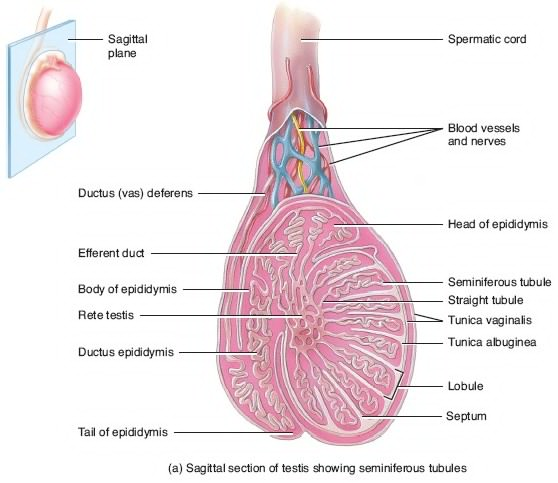
\includegraphics[scale=0.65]{figure/coupe_testicule2} 
  
  }
  
  \caption{Schéma anatomique du testicule humain}\label{fig:testicule}
  \end{figure}
  
  \newpage
  
  \subsection{La phase de
  multiplication}\label{la-phase-de-multiplication}
  
  La phase de multiplication est la phase au cours de laquelle les
  spermatogonies se divisent par mitoses pour aboutir au stade de
  spermatocytes primaires. Les spermatogonies sont des cellules diploïdes
  à l'origine de l'ensemble des autres cellules germinales humaines. Pour
  cela, elles vont s'auto-renouveler par mitoses successives afin de
  maintenir une production continue de spermatozoïdes tout au long de la
  vie de l'individu. Ces cellules sont localisées dans le compartiment
  basal des tubes séminifères. Les analyses histologiques ont permis de
  distinguer trois types de spermatogonies en fonction de leur contenu en
  hétérochromatine (Clermont, \protect\hyperlink{ref-Clermont1963}{1963},
  Clermont (\protect\hyperlink{ref-Clermont1966}{1966}), Goossens \&
  Tournaye (\protect\hyperlink{ref-Goossens2013}{2013})) : Les
  spermatogonies de type A dark (ou Ad), les spermatogonies de type A pale
  (ou Ap) et les spermatogonies de type B.
  
  Chez l'Homme, les spermatogonies Ad ont une activité mitotique au cours
  de la spermatogénèse et servent de réserve. Elles vont au cours d'une
  première mitose former une spermatogonie Ad et un spermatogonie Ap
  (\textbf{Figure :} \ref{fig:spermatogenese}). Cette propriété permet à
  la fois de se différencier en spermatocytes tout en constituant un
  compartiment de réserve de spermatogonies Ad pour la régénération de la
  population de cellules germinales au sein de l'épithélium séminifère.
  L'entrée en division des spermatogonies Ap se fait par groupes
  cellulaire tous les 16 jours. Les cellules d'une même génération
  maintiennent entre elles des ponts cytoplasmiques jusqu'à la
  \protect\hyperlink{spermiogenese}{spermiogénèse} ce qui permet la
  synchronisation parfaite du développement gamétique de toutes les
  cellules filles issues d'un groupe de spermatogonies Ap. Ce phénomène
  est appelé onde spermatogénétique. Chaque spermatogonie Ap va,
  lorsqu'elle se divise par mitose, former deux spermatogonies B qui
  elles-mêmes se diviseront en deux spermatocytes primaires diploïdes
  (\textbf{Figure :} \ref{fig:spermatogenese}).
  
  \newpage
  
  \begin{figure}
  
  {\centering 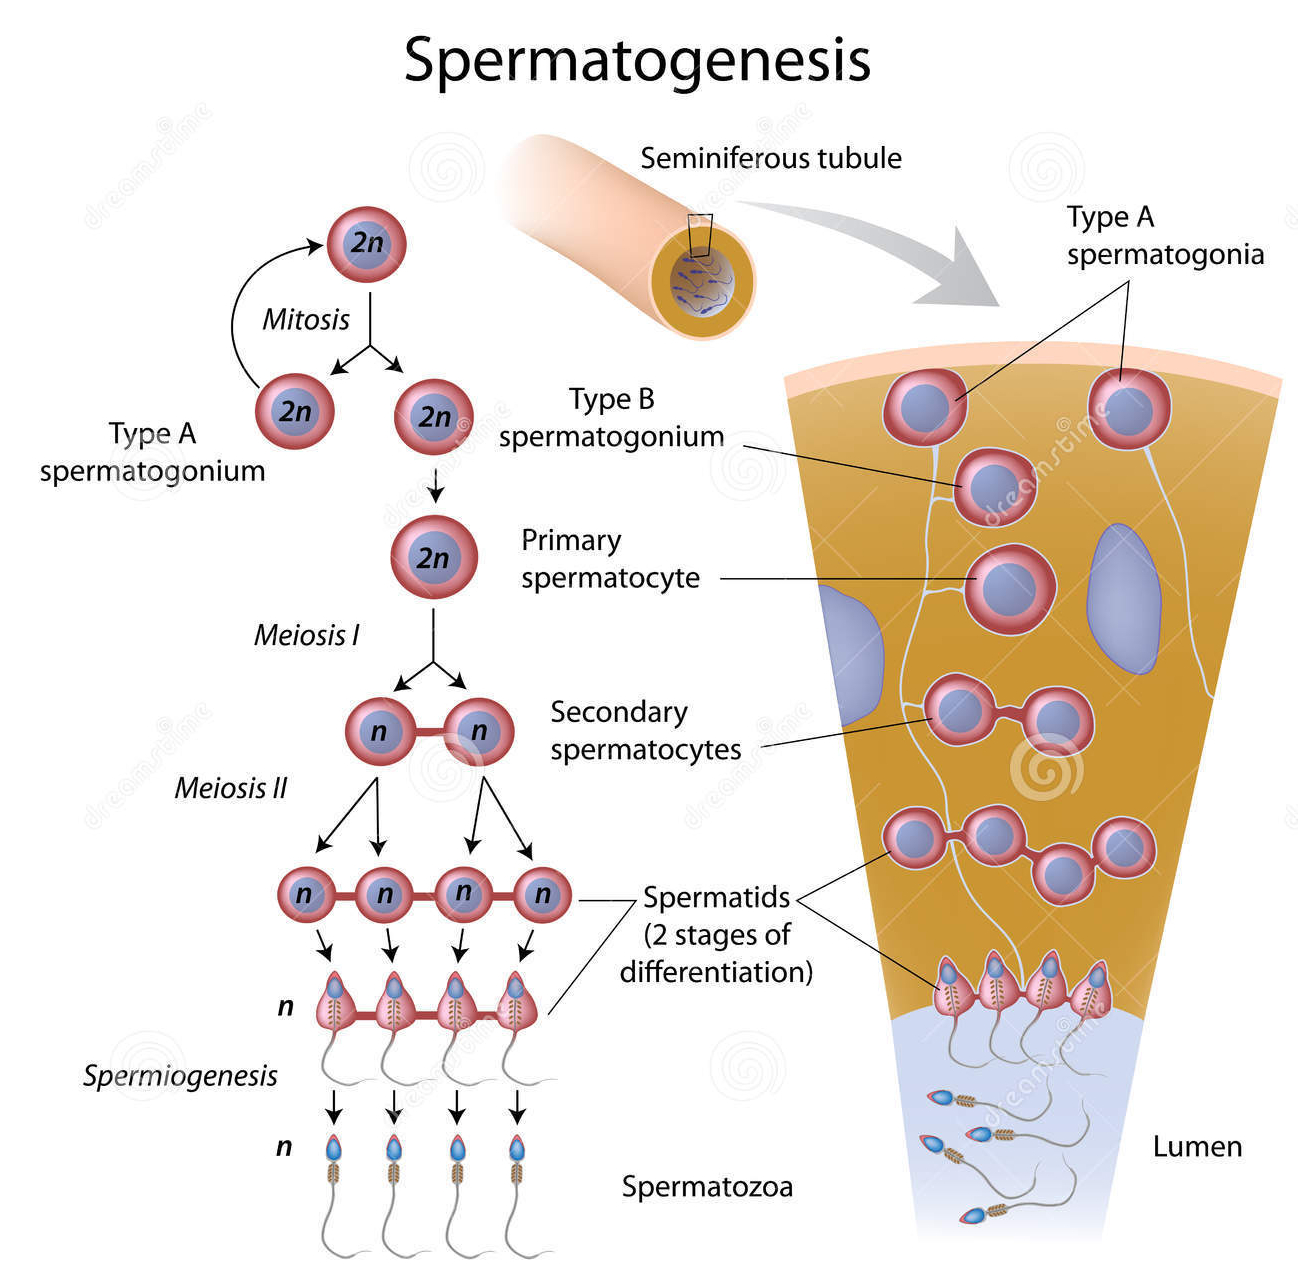
\includegraphics[scale=0.35]{figure/spermatogenese2} 
  
  }
  
  \caption{Les différentes phases de la spermatogénèse d'après [medizin-kompakt](http://www.medizin-kompakt.de/spermatogenese) : description à écrire !!!}\label{fig:spermatogenese}
  \end{figure}
  
  \newpage 
  
  \hypertarget{meiose}{\subsection{La méiose}\label{meiose}}
  
  La méiose, ou phase de maturation, est l'étape au cours de laquelle, à
  partir de cellules diploïdes (les spermatogonies B) vont se former des
  cellules haploïdes, les spermatocytes secondaires (spermatocytes II). Ce
  résultat est le fruit de deux divisions successives (\textbf{Figure :
  }\ref{fig:meiose}) appelée respectivement méiose réductionnelle ou
  méiose I (MI) et méiose équationnelle ou méiose II (MII). La MI va
  séparer les chromosomes homologues, produisant deux cellules et
  réduisant la ploïdie de diploïde à haploïde (d'où son non
  \emph{réductionnelle}). En plus de son rôle de division vu précédemment,
  la méiose joue un rôle clef dans le brassage génétique (mélange des
  gènes) et ce, grâce à deux mécanismes de brassage : le brassage
  inter-chromosomique, lorsque les chromosomes sont séparés et le brassage
  intra-chromosomique impliquant notamment des enjambements chromosomiques
  (crossing-over) (\textbf{Figure : }\ref{fig:crossingover}).
  
  La méiose est initiée dès la fin de la phase de multiplication à partir
  des spermatocytes primaires issus de la division des spermatogonies de
  type B. Ces cellules nouvellement formées se situent dans le
  compartiment basal du tube séminifère. C'est là qu'ils vont tout d'abord
  subir une interphase (stade préleptotène) durant entre 2 et 4 jours. Au
  cours de cette phase a lieu la réplication de l'ADN. Cette réplication
  se fait lorsque l'ADN est à l'état de chromatine, pendant la phase S
  (pour synthèse) de l'interphase. À l'issue de cette phase, chaque
  chromosome sera composé de deux chromatides reliées entre elles par le
  centromère, le matériel génétique de chaque cellule ayant donc été
  multiplié par 2. Par la suite, ces cellules vont subir deux divisions
  méiotiques, chacune composées de 4 étapes distinctes (\textbf{Figure :
  }\ref{fig:meiose}) :
  
  \begin{figure}
  
  {\centering 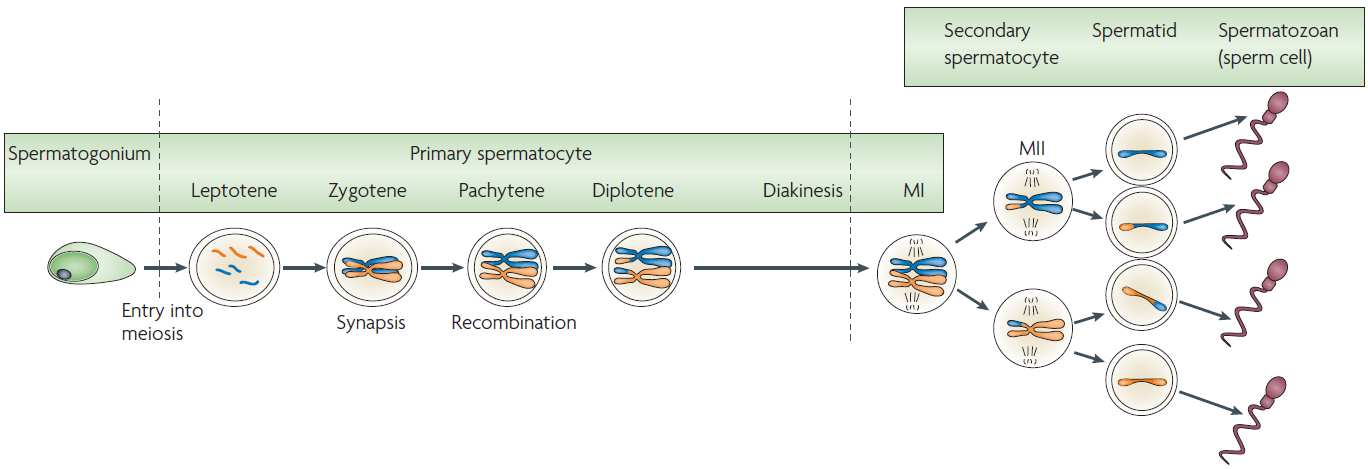
\includegraphics[scale=0.33]{figure/Meiosis_Stages} 
  
  }
  
  \caption[Les différentes étapes de la méiose gamétique masculine]{Les différentes étapes de la méiose gamétique masculine d'après Sasaki et Matsui, 2008}\label{fig:meiose}
  \end{figure}
  
  \newpage
  
  \begin{enumerate}
  \def\labelenumi{\arabic{enumi}.}
  \tightlist
  \item
    \textbf{Méiose réductionnelle} : (\textbf{Figure : }\ref{fig:meiosei})
  
    \begin{enumerate}
    \def\labelenumii{\alph{enumii}.}
    \item
      \textbf{La prophase I} : Cette longue étape dure 23 jours chez
      l'homme et peut être subdivisée en 5 phases successives : leptotène,
      zygotène, pachytène, diplotène et diacinèse.
  
      \begin{enumerate}
      \def\labelenumiii{\roman{enumiii}.}
      \tightlist
      \item
        \textbf{Leptotène} : condensation de la chromatine et formation
        des chromosomes.\\
      \item
        \textbf{Zygotène} : Appariement des chromosomes homologues par
        paires appelées bivalents grâce l'intermédiaire d'une structure
        multi-protéique : le complexe synaptonémal.\\
      \item
        \textbf{Pachytène} : Ce stade dure 16 jours et est le plus long de
        la prophase I. C'est au cours de celui-ci qu'à lieu l'échange de
        matériel génétique par le biais des crossing-over entre les
        chromatides non-sœurs appelés nodules de recombinaison
        (\textbf{Figure : }\ref{fig:crossingover}).\\
      \item
        \textbf{Diplotène} : La dissociation du complexe synaptonémal va
        permettre aux chromosomes homologues d'initier leur séparation.
        Certains sites d'appariement étroits nommés chiasmas demeurent
        néanmoins liés permettant une séparation plus progressive des
        chromosomes et réduisant ainsi le risque d'aneuploïdies (nombre
        anormal de chromosomes) (Handyside,
        \protect\hyperlink{ref-Handyside2012}{2012}).\\
      \item
        \textbf{Diacinèse} : Cette étape marque la fin de la méiose I et
        fait office de transition avec la méiose II. Elle est caractérisée
        par une condensation maximale des chromosomes et la disparition de
        la membrane nucléaire et du nucléole. Le fuseau méiotique commence
        à s'assembler, les centromères des chromosomes homologues
        s'éloignent et les chiasmas glissent progressivement vers les
        télomères.\\
      \end{enumerate}
    \item
      \textbf{La métaphase I} : phase au cours de laquelle les chromosomes
      vont s'aligner à l'équateur de la cellule pour former la plaque
      équatoriale.
    \item
      \textbf{L'anaphase I} : les chromatides sœurs (ou les chromosomes
      homologues en fonction de la phase méiotique) vont se séparer et
      migrer aux pôles opposés de la cellule.\\
    \item
      \textbf{La télophase I} : qui est l'étape finale, les chromosomes se
      décondensent et l'enveloppe nucléaire se reforme autours des
      chromosomes. La cellule mère se sépare alors en deux cellules filles
      appelées spermatocytes secondaires.
    \end{enumerate}
  \end{enumerate}
  
  \newpage
  
  \begin{enumerate}
  \def\labelenumi{\arabic{enumi}.}
  \setcounter{enumi}{1}
  \tightlist
  \item
    \textbf{Méiose équationnelle} : (\textbf{Figure : }\ref{fig:meioseii})
    La MII est similaire à une division mitotique et peut se décomposer en
    4 parties distinctes :
  
    \begin{enumerate}
    \def\labelenumii{\alph{enumii}.}
    \tightlist
    \item
      \textbf{La prophase II} : Contrairement à la prophase I, la prophase
      II est très courte. Les chromosomes alors formés de deux chromatides
      sœurs se dirigent vers la plaque équatoriale.\\
    \item
      \textbf{La métaphase II} : À ce stade, les chromosomes sont alignés
      le long de la plaque équatoriale au niveau de leur centromère.\\
    \item
      \textbf{L'anaphase II} : Les centromères de chaque chromosome se
      séparent permettant aux chromatides sœurs de se diriger vers les
      pôles opposés des spermatocytes II.\\
    \item
      \textbf{La télophase II} : Comme en télophase I, les cellules mères
      se séparent en deux cellules filles haploïdes appelées spermatides,
      contenant chacune n chromosomes.
    \end{enumerate}
  \end{enumerate}
  
  \begin{figure}
  
  {\centering 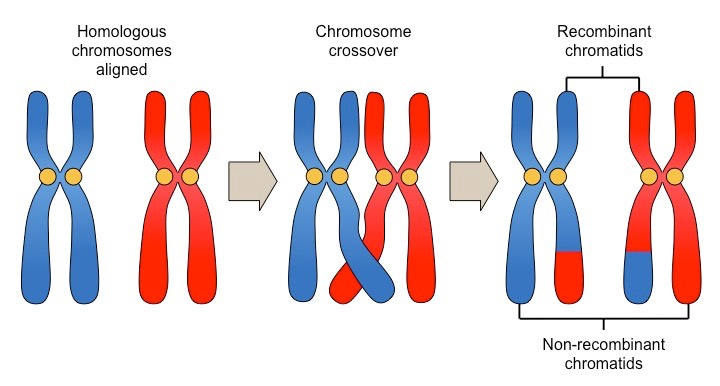
\includegraphics[scale=0.35]{figure/crossingover} 
  
  }
  
  \caption{Schéma simplifié d'un enjambement chromosomique (crossing-over)}\label{fig:crossingover}
  \end{figure}
  
  \newpage 
  
  \begin{figure}
  
  {\centering 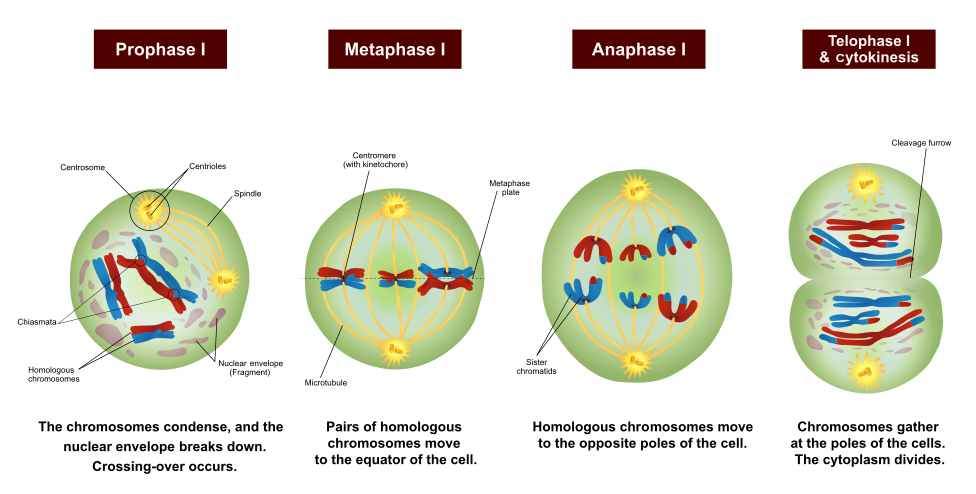
\includegraphics[scale=0.43]{figure/MeiosisI} 
  
  }
  
  \caption[Les différentes étapes de la première division méiotique masculine adapté]{Les différentes étapes de la première division méiotique masculine adapté d'après [Wikipédia](https://en.wikipedia.org/wiki/Meiosis)}\label{fig:meiosei}
  \end{figure}
  
  \begin{figure}
  
  {\centering 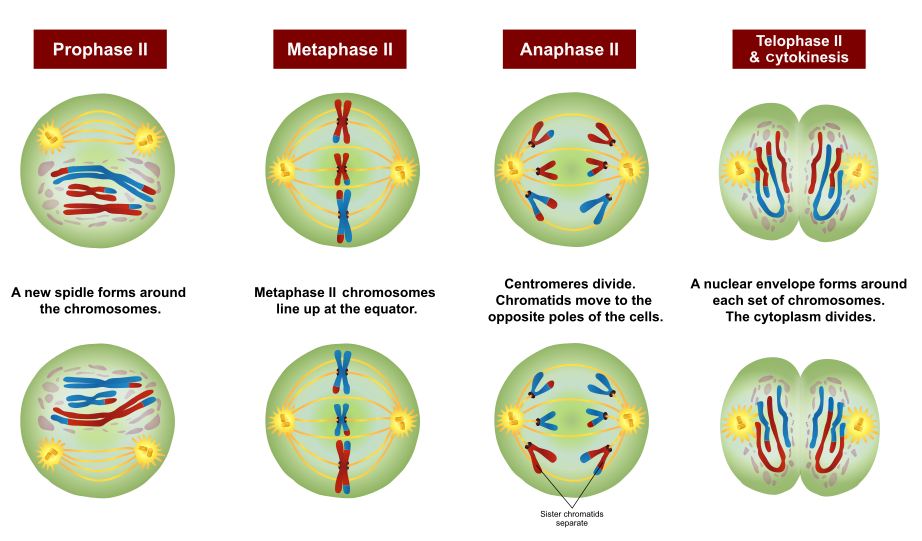
\includegraphics[scale=0.43]{figure/MeiosisII} 
  
  }
  
  \caption[Les différentes étapes de la deuxième division méiotique masculine adapté]{Les différentes étapes de la deuxième division méiotique masculine adapté d'après [Wikipédia](https://en.wikipedia.org/wiki/Meiosis)}\label{fig:meioseii}
  \end{figure}
  
  \newpage
  
  \hypertarget{spermiogenese}{\subsection{La
  spermiogénèse}\label{spermiogenese}}
  
  La spermiogénèse est la phase finale de la spermatogénèse. Elle dure
  environ 23 jours chez l'humain et peut être subdivisée en sept étapes
  (\textbf{Figure : }\ref{fig:spermiogenese}). La spermiogénèse définie la
  cytodifférentiation des spermatides en spermatozoïdes. C'est au cours de
  cette phase que les caractéristiques morphologiques et fonctionnelles du
  spermatozoïde seront déterminées (Yves Clermont, Richard Oko,
  \protect\hyperlink{ref-YvesClermontRichardOko1993}{1993}). Elle est
  caractérisée par 3 évènements majeurs : la formation de l'acrosome, la
  compaction de l'ADN nucléaire et la formation du flagelle. Le
  développement de l'acrosome et la formation du flagelle commencent au
  niveau des spermatides rondes (D. Escalier et al.,
  \protect\hyperlink{ref-Escalier1991}{1991}). Pendant l'élongation de la
  spermatide, le noyau se condense et devient hautement polarisé
  (Hamilton, D. W., Waites, \protect\hyperlink{ref-Hamilton1987}{1990}).\\
  Les spermatides sont situées dans le compartiment adluminal, à proximité
  de la lumière du tube séminifère. Ce sont de petites cellules (8 à 10
  \(\upmu\)m) que l'on peut schématiquement diviser en trois classes :
  
  \begin{enumerate}
  \def\labelenumi{\arabic{enumi}.}
  \item
    \textbf{Les spermatides rondes} (\textbf{Figure :
    }\ref{fig:spermiogenese} - \textbf{1} et \textbf{2}) :
    L'identification de ces cellules représente une difficulté technique.
    Elles ont cependant pu être décrites en détail par différentes
    techniques de coloration sous microscope optique (Clermont,
    \protect\hyperlink{ref-Clermont1963}{1963}, Papic, Katona, \& Skrabalo
    (\protect\hyperlink{ref-Papic}{1988}), Schenck \& Schill (n.d.),
    Adelman \& Cahill (\protect\hyperlink{ref-Adelman1989}{1989}), World
    Health Organization
    (\protect\hyperlink{ref-WorldHealthOrganization1992}{1992})).
    Plusieurs études animales ont pu démontrer le potentiel des
    spermatides rondes à donner la vie à des individus sains et fertiles,
    (a Ogura, Matsuda, \& Yanagimachi,
    \protect\hyperlink{ref-Ogura1994}{1994}, A. Ogura, Matsuda, Asano,
    Suzuki, \& Yanagimachi (\protect\hyperlink{ref-Kimura1995}{1996}),
    Sasagawa \& Yanagimachi (\protect\hyperlink{ref-Sasagawa}{1997})), la
    même chose ayant été également observée plus récemment chez l'homme
    (A. Tanaka et al., \protect\hyperlink{ref-Tanaka2015}{2015}) bien que
    le taux de fécondation et d'implantation soit extrêmement faible
    (Asimakopoulos, \protect\hyperlink{ref-Asimakopoulos2003}{2003}). Ils
    possèdent un noyau rond avec une chromatine pâle et homogène. C'est à
    partir de ces étapes que démarre la biogenèse de l'acrosome avec la
    production par l'appareil de Golgi des vésicules pro-acrosomales
    (phase de Golgi). Les deux centrioles contenus dans le cytoplasme vont
    se déplacer au futur pôle caudal. Le centriole proximal est inactif
    alors que le centriole distal donne naissance à un ensemble de
    microtubules à l'origine de l'axonème du futur flagelle.
  \item
    \textbf{Les spermatides en élongation} (\textbf{Figure :
    }\ref{fig:spermiogenese} - \textbf{3} et \textbf{4}) : À ce stade,
    l'acrosome va s'étendre le long du noyau lui donnant une forme plus
    allongée et la chromatine devient plus sombre. Un réseau de
    microtubule se forment autours du noyau créant ainsi la manchette qui
    participera également à l'allongement de la tête du spermatozoïde et
    permettra la migration des mitochondries vers la pièce intermédiaire
    du flagelle former le manchon de mitochondries (Moreno, Palomino, \&
    Schatten, \protect\hyperlink{ref-Moreno2006}{2006}). Les spermatides
    en élongation peuvent aussi permettre la fécondation et d'initier des
    grossesses avec un meilleur taux que les spermatides rondes et
    engendreraient théoriquement moins de risques d'anomalies génétiques
    (Asimakopoulos, \protect\hyperlink{ref-Asimakopoulos2003}{2003}).
  \end{enumerate}
  
  \newpage
  
  \begin{enumerate}
  \def\labelenumi{\arabic{enumi}.}
  \setcounter{enumi}{2}
  \tightlist
  \item
    \textbf{Les spermatides en condensation} (\textbf{Figure :
    }\ref{fig:spermiogenese} - \textbf{5} et \textbf{7}) : C'est le stade
    final de la différentiation de la spermatide en spermatozoïde. À ce
    stade le noyau est très allongé, avec une partie caudale globulaire et
    une partie antérieure saillante. La chromatine est sombre et
    condensée. L'axonème va continuer à s'allonger pour former le flagelle
    mature. Les différentes organelles inutiles pour la physiologique
    spermatique et l'excès de cytoplasme vont former la gouttelette
    cytoplasmique qui va se détacher et donner le corps résiduel qui va
    ensuite être phagocyté par les cellules de Sertoli (Hermo, Pelletier,
    Cyr, \& Smith, \protect\hyperlink{ref-Hermo2010}{2010}).
  \end{enumerate}
  
  Une fois ces étapes de différentiation finies, les spermatides sont
  relâchées en tant que spermatozoïdes dans la lumière du tube séminifère.
  Ce procédé est appelé spermiation.
  
  \begin{figure}
  
  {\centering 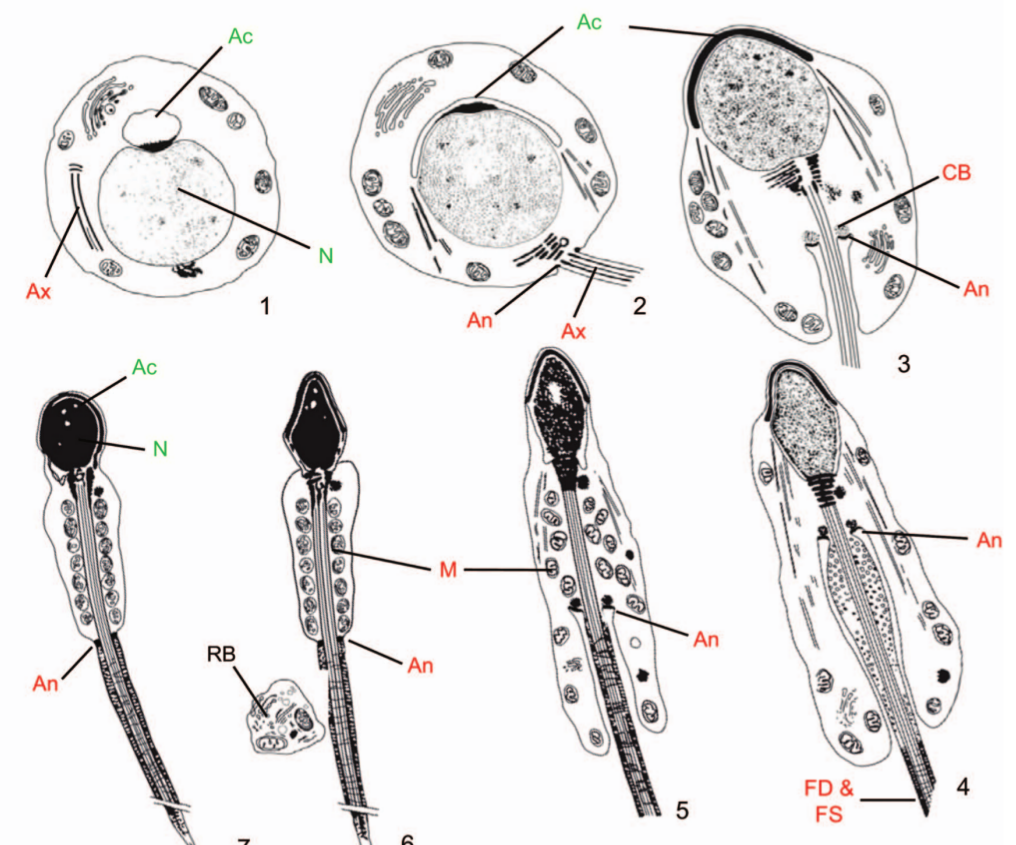
\includegraphics[scale=0.3]{figure/spermiogenese} 
  
  }
  
  \caption[Principales étapes et modifications structurales lors de la spermiogénèse]{Principales étapes et modifications structurales lors de la spermiogénèse : 1. La spermatide immature avec un gros noyau arrondi. La vésicule acrosomale est attachée au noyau, l’ébauche du flagelle n’atteint pas le noyau. 2. La vésicule acrosomale a augmenté de taille et apparaît aplatie au niveau du noyau. Le flagelle entre en contact avec le noyau. 3-7. Formation de l’acrosome, condensation du noyau et développement des structures flagellaires. Ac, acrosome ; Ax, axonème ; CC, corps chromatoïdes ; CR, corps résiduel ; FD, fibres denses ; GF, gaine fibreuse ; M, mitochondrie ; Ma, manchette. d'après [@Toure2011]}\label{fig:spermiogenese}
  \end{figure}
  
  \newpage  
  
  \section{Structure et fonction du
  spermatozoïde}\label{structure-et-fonction-du-spermatozoide}
  
  Le spermatozoïde est une cellule hautement différenciée dont la taille,
  l'orientation et la symétrie sont déterminées. La morphologie générale
  du spermatozoïde éjaculé est similaire à celle du spermatozoïde
  testiculaire. Le spermatozoïde humain normal mature mesure environ 60
  \(\upmu\)m de long et est essentiellement constitué de deux parties : la
  tête et le flagelle (\textbf{Figure : }\ref{fig:spz}). En plus d'être
  unique dans sa morphologie, le spermatozoïde l'est aussi dans sa
  fonction puisque c'est la seule cellule produite de manière endogène et
  dont l'action est exercée de manière exogène. La fécondation d'un
  ovocyte par un spermatozoïde formera un zygote diploïde qui pourrase
  développer ensuite en embryon dans l'uterus féminin.
  
  \begin{figure}
  
  {\centering 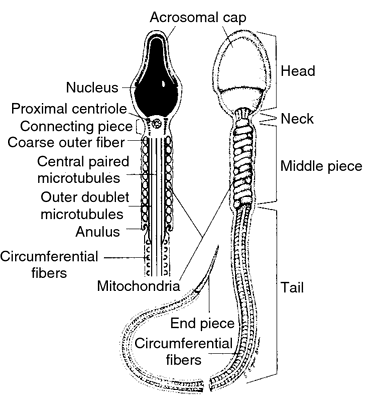
\includegraphics[scale=.75]{figure/sperm_anatomy} 
  
  }
  
  \caption[Anatomie simplifiée du spermatozoïde]{Anatomie simplifiée du spermatozoïde}\label{fig:spz}
  \end{figure}
  
  \newpage
  
  \subsection{La tête}\label{la-tete}
  
  \begin{enumerate}
  \def\labelenumi{\arabic{enumi}.}
  \tightlist
  \item
    \textbf{L'acrosome} : C'est une vésicule de sécrétion géante située
    dans la moitié supérieure de la tête du spermatozoïde. Elle se
    développe à partir de l'appareil de Golgi lors de la spermiogénèse. Au
    cours de sa formation, l'acrosome forme tout d'abord un granule
    sphérique qui se colle sur la partie apicale du noyau. En
    s'aplatissant contre celui-ci, l'acrosome va prendre une forme
    hémisphérique recouvrant la membrane nucléaire formant la coiffe
    céphalique. Le rôle de l'acrosome est fondamental dans le processus de
    fécondation puisqu'il permet d'excréter notamment l'acrosine, une
    enzyme de digestion permettant au spermatozoïde de traverser la zone
    pellucide qui entoure les ovocytes. Ce processus de relargage est
    appelé réaction acrosomale.\\
  \item
    \textbf{L'acroplaxome} : L'acroplaxome est une structure cytosquelette
    composée de microfilaments d'actine (F- actine) et de kératine 5.
    Cette structure est positionnée en face de l'appareil de golgi et
    contre le noyau et sert de point d'attachement ainsi que de guide aux
    vésicules pro-acrosomales (Abraham L Kierszenbaum \& Tres,
    \protect\hyperlink{ref-Kierszenbaum2004}{2004}). C'est une structure
    transitoire qui disparaît pour être remplacée par la thèque
    périnucléaire dans le spermatozoïde mature.\\
  \item
    \textbf{Le noyau} : C'est une structure cellulaire présente dans la
    majorité des cellules eucaryotes. Il contient l'essentiel du matériel
    génétique. Le noyau du spermatozoïde est caractérisé par une
    compaction extrêmement importante de l'ADN. Dans les cellules
    somatiques l'ADN est enroulé par unité de 146 paires de bases autour
    d'un octamère d'histones dit de cœur (H2A, H2B, H3 et H4) afin
    d'organiser les 3 milliards de paires de bases du génome humain dans
    un noyau de quelques microns (\textbf{Figure : }\ref{fig:noyau}).
    L'ADN des spermatides va subir une réorganisation chromatinienne plus
    importante au cours de la spermatogénèse afin d'augmenter sa
    compaction. Ainsi, les octamères d'histones présents dans les cellules
    somatiques sont remplacés par les protéines de transition (TPN1, TPN2)
    puis par les protamines (PRM1, PRM2) deux protéines riches en arginine
    et en cystéine (\textbf{Figure : }\ref{fig:noyau}). L'intégrité des
    deux protéines composant ce dimère est nécessaire pour la procréation
    (C. Cho et al., \protect\hyperlink{ref-Cho2001}{2001}). Cette
    compaction extrême permet de réduire la taille du noyau, mais aussi de
    protéger l'ADN d'agents de dégradation comme l'oxydation des bases.
    Parallèlement à cette condensation chromatinienne se produit un arrêt
    des processus de transcription cellulaire (A L Kierszenbaum \& Tres,
    \protect\hyperlink{ref-Kierszenbaum1978}{1978}). Le noyau du
    spermatozoïde est donc un noyau au repos, transcriptionnellement
    inactif (Ward, \protect\hyperlink{ref-Ward1994}{1994})
  \end{enumerate}
  
  \newpage
  
  \begin{figure}
  
  {\centering 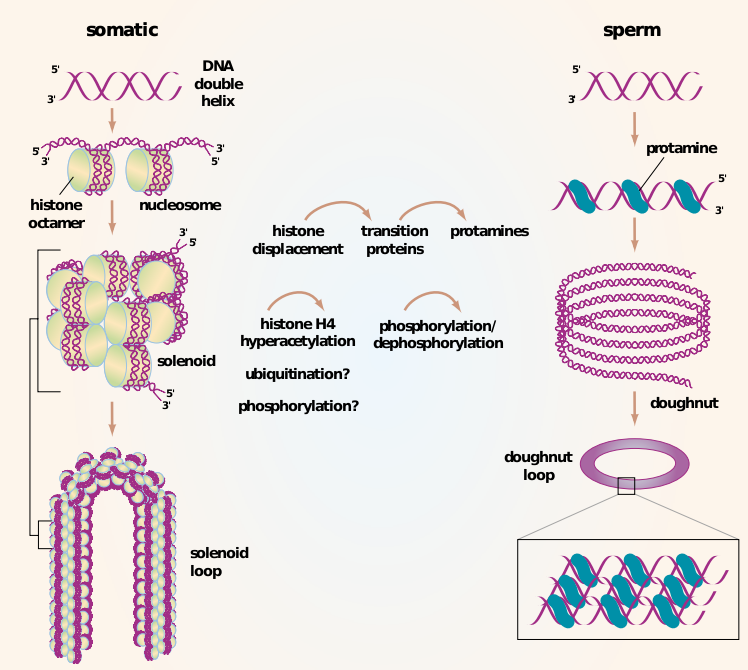
\includegraphics[scale=.55]{figure/noyau} 
  
  }
  
  \caption[Schéma de la compaction de l’ADN dans les cellules somatiques et dans les spermatozoïdes]{Schéma de la compaction de l’ADN dans les cellules somatiques et dans les spermatozoïdes : D'après Braun (2001)}\label{fig:noyau}
  \end{figure}
  
  \newpage
  
  \subsection{Le flagelle}\label{le-flagelle}
  
  Le flagelle représente la queue du spermatozoïde. Celui-ci permet, par
  mouvement d'oscillation à haute vitesse, le déplacement du
  spermatozoïde. Cette mobilité est générée par un cytosquelette interne
  extrêmement conservé durant l'évolution appelé l'axonème. Celui-ci est
  composé de neuf doublets de microtubules périphériques et de deux
  doublets internes (Inaba, \protect\hyperlink{ref-Inaba2003}{2003})
  (\textbf{Figure : }\ref{fig:axoneme}), on parle alors de structure ``9 +
  2''. Les doublets externes sont reliés entre eux par des ponts de nexine
  et au doublet central par des ponts radiaires. Les doublets externes
  sont également reliés entre eux par les complexes protéiques qui forment
  les dynéines externes et internes. Ce sont ces protéines qui en exerçant
  une contraction alternée permettent le mouvement du spermatozoïde.
  
  \begin{figure}
  
  {\centering 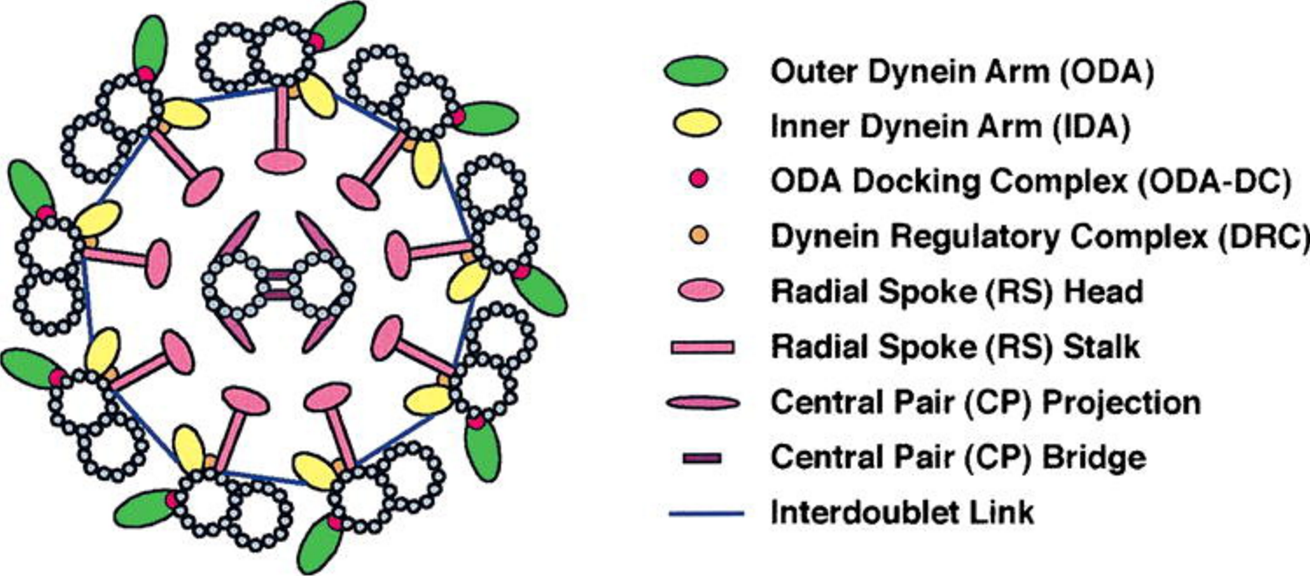
\includegraphics[scale=.3]{figure/axoneme} 
  
  }
  
  \caption[Structure simplifiée de l'axonème]{Structure simplifiée de l'axonème d'après [@Inaba2003] : L'axonème est constitué de neuf doublets de microtubules périphériques reliés entre eux par des liens de nexine et d'un doublet central relié aux doublets périphériques par des ponts radiaires}\label{fig:axoneme}
  \end{figure}
  
  Le flagelle du spermatozoïde peut être divisé en trois partie distinctes
  (\textbf{Figure : }\ref{fig:flagelle}) :
  
  \begin{enumerate}
  \def\labelenumi{\arabic{enumi}.}
  \tightlist
  \item
    \textbf{La pièce intermédiaire} : Elle fait jonction avec la tête du
    spermatozoïde et est composée de la gaine de mitochondrie qui fournira
    une partie de de l'énergie nécessaire au battement flagellaire (grâce
    à la phosphorylation oxydative qui produit de l'ATP). L'axonème qui se
    prolonge dans la pièce principale et un ensemble de neuf faisceaux de
    fibres denses.
  \end{enumerate}
  
  \newpage
  
  \begin{enumerate}
  \def\labelenumi{\arabic{enumi}.}
  \setcounter{enumi}{1}
  \tightlist
  \item
    \textbf{La pièce principale} : Ici, la gaine de mitochondrie a
    disparue ainsi que deux des faisceaux de fibres denses présents dans
    la pièce intermédiaire. On note cependant la présence d'une structure
    supplémentaire, la gaine fibreuse. Cette gaine entoure l'axonème et
    comporte deux épaississements diamétralement opposés, appelés colonnes
    longitudinales sur lesquelles s'insèrent les fibres denses 3 et 8.
    C'est le long de la gaine fibreuse qu'est produit la majorité de
    l'énergie nécessaire au glissement des microtubules (Eddy,
    \protect\hyperlink{ref-Eddy2007}{2007}).\\
  \item
    \textbf{La pièce terminale} : Elle est située au niveau de l'extrémité
    distale du flagelle et ne contient que l'axonème (Inaba,
    \protect\hyperlink{ref-Inaba2003}{2003}).
  \end{enumerate}
  
  \begin{figure}
  
  {\centering 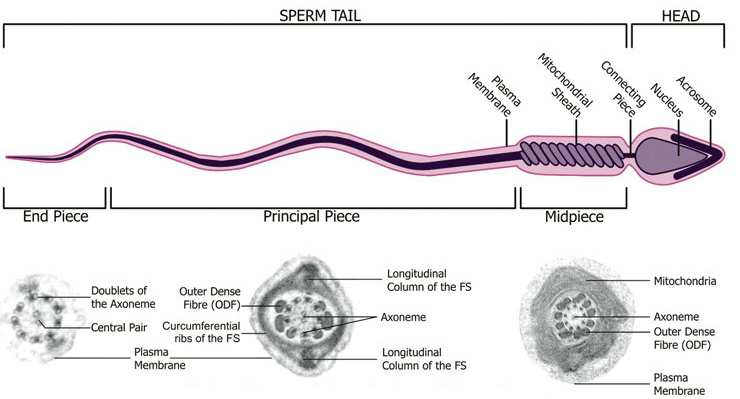
\includegraphics[scale=.55]{figure/sperm2} 
  
  }
  
  \caption[Structure du flagelle d’un spermatozoïde]{Structure du flagelle d’un spermatozoïde d'après Borg et al. (2010) : Coupes transversales en microscopie électronique. Le flagelle se compose de trois parties : la pièce intermédiaire, contenant les mitochondries, la pièce principale et la pièce terminale. L’axonème, en position centrale, parcours tout le flagelle. Des structures périaxonèmales sont observables : les fibres denses dans la pièce intermédiaire et principale, et la gaine fibreuse dans la pièce principale seulement.}\label{fig:flagelle}
  \end{figure}
  
  \newpage
  
  \section{L'infertilité masculine}\label{linfertilite-masculine}
  
  L'organisation mondiale de la santé définie l'infertilité comme étant :
  ``\emph{une pathologie du système reproductif définie par l'échec d'une
  grossesse clinique après 12 mois ou plus de rapports sexuels réguliers
  non protégés}''
  (\href{http://www.who.int/reproductivehealth/topics/infertility/definitions/en/}{\texttt{Who.int.\ 2013-03-19.\ Retrieved\ 2013-06-17}}).
  L'étude de l'infertilité représente un des enjeux scientifique et
  médical majeur de ces dernières années. On estime qu'environ 10 à 15\%
  des couples humains font face à des problèmes d'infertilité soit plus de
  70 millions de personnes dans le monde (Boivin, Bunting, Collins, \&
  Nygren, \protect\hyperlink{ref-Boivin2007a}{2007}). Dans la moitié des
  cas, la cause sous-jacente serait masculine. On estime que les facteurs
  causaux sous-jacents de l'infertilité masculine peuvent être attribués à
  des toxines environnementales, des troubles systémiques tels que la
  maladie hypothalamo-hypophysaire, les cancers testiculaires et l'aplasie
  des cellules germinales. Les facteurs génétiques, y compris les
  aneuploïdies et les mutations de gènes uniques, contribuent également à
  l'infertilité masculine. Cependant, aucune cause n'est identifiée dans
  près de la moitié des cas. Comme nous avons pu le voir, la
  spermatogénèse est une succession de processus complexes qui s'effectue
  de manière coordonnée, de fait la moindre altération génétique affectant
  une seule de ces étapes est susceptible d'entrainer un phénotype
  d'infertilité (Grudzinskas \& Yovich,
  \protect\hyperlink{ref-Grudzinskas1995}{1995}).
  
  \subsection{Les différents phénotypes d'infertilité
  masculine}\label{les-differents-phenotypes-dinfertilite-masculine}
  
  Chez l'homme, l'infertilité est associée à une altération quantitative
  et / ou qualitative des spermatozoïdes présents dans l'éjaculat.
  L'ensemble de ces altérations peuvent être détectées et quantifiées dans
  des laboratoires spécialisés par réalisation d'un spermogramme. Au cours
  de celui-ci, plusieurs critères tels que le volume de sperme sécrété,
  son pH, la quantité et la vitalité des spermatozoïdes qu'il contient
  seront évalués. La proportion de cellules immatures sera elle aussi
  analysée. Ces cellules rondes, se retrouvent à la fois dans l'éjaculat
  des individus ayant une quantité de spermatozoïdes ``normale'' (Michael
  \& Joel, \protect\hyperlink{ref-Michael1937}{1937},M. Tomlinson et al.
  (\protect\hyperlink{ref-Tomlinson1993a}{1993})), chez les individus
  présentant une quantité basse de spermatozoïdes (MacLeod,
  \protect\hyperlink{ref-MacLeod1970}{1970}, M. J. Tomlinson, Barratt, \&
  Cooke (\protect\hyperlink{ref-Tomlinson1993}{1993})) ou en étant
  dépourvu (Kurilo, Liubashevskaia, Dubinskaia, \& Gaeva,
  \protect\hyperlink{ref-Kurilo}{1993}). Cependant, leur nombre augmente
  tandis que la quantité de spermatozoïde diminue (SPERLING \& KADEN,
  \protect\hyperlink{ref-SPERLING1971}{1971}).
  
  \newpage
  
  \hypertarget{infquant}{\subsubsection{Anomalies liées à la quantité
  spermatique}\label{infquant}}
  
  Chez l'humain, l'arrêt de la spermatogénèse est défini comme
  l'incapacité des cellules spermatogénétiques à devenir des
  spermatozoïdes matures. Elle peut survenir à n'importe quelle étape de
  la formation des cellules germinales. Les blocages méiotiques, au stade
  de spermatocyte I sont les plus fréquents, suivis par l'arrêt au niveau
  des spermatides et moins fréquemment au niveau des spermatogonies
  (Girgis, Etriby, Ibrahim, \& Kahil,
  \protect\hyperlink{ref-Girgis}{1969}).
  
  \begin{enumerate}
  \def\labelenumi{\arabic{enumi}.}
  \tightlist
  \item
    \textbf{L'oligozoospermie} : L'oligozoospermie est définie comme un
    phénotype d'infertilité masculine caractérisé par une production
    inférieure à 15 millions de spermatozoïdes par ml de sperme (T. G.
    Cooper et al., \protect\hyperlink{ref-Cooper2010}{2010}). Un arrêt de
    la spermatogénèse a été observé dans 4 à 30\% des biopsies
    testiculaires des hommes présentant une oligospermie sévère (Colgan,
    Bedard, Strawbridge, Buckspan, \& Klotz,
    \protect\hyperlink{ref-Colgan1980}{1980}, Levin
    (\protect\hyperlink{ref-Levin1979}{1979}), Soderström \& Suominen
    (\protect\hyperlink{ref-Soderstrom1980}{1980}), WONG, STRAUS, \&
    WARNER (\protect\hyperlink{ref-WONG1973}{1973})). Cet arrêt a
    longtemps été considéré comme sans espoir pour les couples désirant
    concevoir, jusqu'à l'émergence de l'injection mécanique d'un
    spermatozoïde dans l'ovocyte appelé \emph{intracytoplasmic sperm
    injection} (ICSI) (Palermo, Joris, Devroey, \& Van Steirteghem,
    \protect\hyperlink{ref-Palermo1992}{1992})\\
  \item
    \textbf{L'azoospermie} : Comme l'oligozoospermie, l'azoospermie est un
    phénotype d'infertilité masculine cette fois-ci caractérisé par
    l'absence totale de spermatozoïdes dans l'éjaculat. On distingue des
    causes excrétoires empêchant l'excrétion des spermatozoïdes, on parle
    alors d'azoospermie obstructive et des causes sécrétoires, les plus
    fréquentes, accompagnées d'un défaut de la spermatogenèse, on parle
    alors d'azoospermie non-obstructive.
  \end{enumerate}
  
  \subsubsection{Anomalies liées liée à la
  morphologie}\label{anomalies-liees-liee-a-la-morphologie}
  
  Ces anomalies sont observables en effectuant un spermocytogramme.
  Plusieurs classifications ont été établies, cependant, c'est la
  classification de David modifiée (\textbf{Table :}
  \ref{fig:anomaliemorphosperm}) qui est la plus rependue en France. Pour
  ce faire, on procède généralement à une observation de 100
  spermatozoïdes au cours de laquelle l'ensemble des anomalies observées
  sont relevées et quantifiées permettant ainsi de définir un index
  d'anomalies multiple (nombre total d'anomalies/nombre de spermatozoïdes
  anormaux) révélant le nombre moyen d'anomalies par spermatozoïdes.
  
  \newpage  
  
  \begin{figure}
  
  {\centering \includegraphics[scale=.75]{figure/tab_sperm_defect} 
  
  }
  
  \caption[Classification morphologique de spermatozoïdes humains normaux et anormaux adapté]{Classification morphologique de spermatozoïdes humains normaux et anormaux adapté d'après [@Auger2001]}\label{fig:anomaliemorphosperm}
  \end{figure}
  
  \newpage
  
  \subsubsection{Anomalies liées à la
  mobilité}\label{anomalies-liees-a-la-mobilite}
  
  Le succès du passage du spermatozoïde le long du tractus génitale
  féminin dépend en grande partie de la mobilité et de la vitesse du
  spermatozoïde (Lindholmer, \protect\hyperlink{ref-Lindholmer1974}{1974},
  Björndahl (\protect\hyperlink{ref-Bjorndahl2010}{2010})). La vitesse
  moyenne d'un spermatozoïde étant de 25 \(\upmu\)m/s. Une mauvaise
  mobilité observée dans plus de 50\% des spermatozoïdes éjaculés se
  révèle être un prédicteur de l'échec de la fécondation (Aitken, Sutton,
  Warner, \& Richardson, \protect\hyperlink{ref-Aitken1985}{1985}).
  
  \subsection{La génétique de
  l'infertilité}\label{la-genetique-de-linfertilite}
  
  Comme il a déjà été dit, il est estimé que 10 à 15\% des couples humain
  font face à des problèmes d'infertilité. Par ailleurs, 30\% des
  infertilités restent inexpliquées et près de 40\% ont des causes
  incertaines. Ainsi, l'infertilité masculine d'origine génétique pourrait
  concerner près de 1 homme sur 40 (Tüttelmann et al.,
  \protect\hyperlink{ref-Tuttelmann2011}{2011}).
  
  \subsubsection{Les causes fréquentes}\label{les-causes-frequentes}
  
  \begin{enumerate}
  \def\labelenumi{\arabic{enumi}.}
  \tightlist
  \item
    \textbf{Les microdélétions du chromosome Y} : Le chromosome Y est un
    petit chromosome atteignant une taille d'environ 53 Mb et est porteur
    de 78 gènes principalement impliqués dans la différentiation sexuelle
    masculine et la spermatogénèse (Skaletsky et al.,
    \protect\hyperlink{ref-Skaletsky2003}{2003}). De fait, le chromosome Y
    représente une région d'intérêt évidente dans l'étude de facteur
    génétique liés à l'infertilité masculine. L'évolution des technologies
    a permis de mettre en évidence des délétions invisibles au caryotype
    dans la région du facteur AZF (\emph{Azoospermia Factor}). Cette
    région peut être subdivisée en trois sous-parties, AZFa, AZFb et AZFc
    (\textbf{Figure :} \ref{fig:chry}). Depuis plusieurs années, de
    nombreuses séries de patients azoospermiques ou oligozoospermiques ont
    été étudiées et publiées et tendent à montrer que les microdélétions
    du chromosome Y seraient responsables de 10\% des cas d'azoospermie
    non-obstructive et chez 5\% des cas d'oligozoospermie sévère
    (\textless{}5 millions de spermatozoïdes/ml) (Hotaling \& Carrell,
    \protect\hyperlink{ref-Hotaling2014}{2014}).
  \end{enumerate}
  
  \newpage
  
  \begin{figure}
  
  {\centering 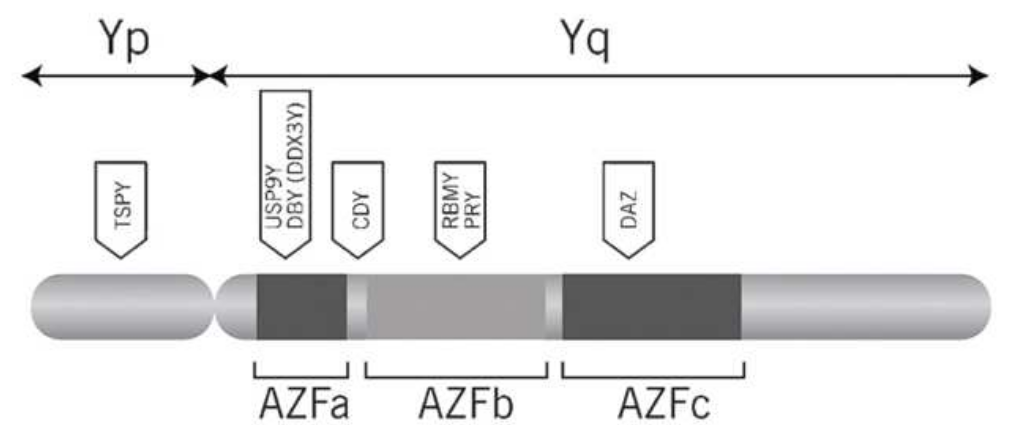
\includegraphics[scale=.45]{figure/chromozomeY} 
  
  }
  
  \caption[Représentation schématique du chromosome Y adapté]{Représentation schématique du chromosome Y adapté d'après [@OFlynnOBrien2010] : Visualisation la région AZF ainsi que des trois sous-régions AZF a, b, c et des principaux gènes compris dans chacune des sous-régions}\label{fig:chry}
  \end{figure}
  
  \begin{enumerate}
  \def\labelenumi{\arabic{enumi}.}
  \setcounter{enumi}{1}
  \tightlist
  \item
    \textbf{Anomalies chromosomiques} : Des anomalies chromosomiques de
    nombre ou de structure impliquant les autosomes ou, le plus souvent,
    les gonosomes, peuvent être impliquées dans des cas d'infertilité
    masculine. Le pourcentage d'individus concernés varie entre 2 et 8\%
    et peut atteindre 15\% pour les patients azoospermiques soit 10 à 20
    fois la fréquence retrouvée dans la population générale (C. Ravel,
    Berthaut, Bresson, Siffroi, \& Genetics Commission of the French
    Federation of CECOS, \protect\hyperlink{ref-Ravel2006}{2006}).
  
    \begin{enumerate}
    \def\labelenumii{\alph{enumii}.}
    \item
      \textbf{Syndrome de Klinefelter} : Le syndrome de Klinefelter (ou
      46, XXY) fut décrit pour la première fois en 1942 par Harry F.
      Klinefelter et décrit une affection due à la présence d'un
      chromosome X supplémentaire suite à une erreur de ségrégation des
      chromosomes au moment de la méiose. Sa prévalence dans la population
      générale est estimée à environ 1 sur 1200 (1 homme sur 600) (Bojesen
      \& Gravholt, \protect\hyperlink{ref-Bojesen2011}{2011}) mais elle
      est environ 50 fois supérieure chez les patients infertiles
      azoospermiques (Gekas et al.,
      \protect\hyperlink{ref-Gekas2001}{2001}).
    \item
      \textbf{Les anomalies de structure} : Les translocations et les
      inversions sont les anomalies de structures retrouvées le plus
      fréquemment chez les patients infertiles.
  
      \begin{enumerate}
      \def\labelenumiii{\roman{enumiii}.}
      \tightlist
      \item
        La translocation est définie comme l'échange de matériel génétique
        entre deux chromosomes non homologues. On en distingue deux types,
        les translocations réciproques et les translocations
        robertsonniennes. Les premières (\textbf{Figure :}
        \ref{fig:figtranslocation} - \textbf{A}) décrivent un échange
        équilibré entre deux mêmes segments chromosomiques de deux
        chromosomes différents. Elles sont retrouvées 4 à 10 fois plus
        fréquemment chez les patients infertiles que dans la population
        générale (D. J. Elliott \& Cooke,
        \protect\hyperlink{ref-Elliott1997}{1997}). Les secondes
        (\textbf{Figure :} \ref{fig:figtranslocation} - \textbf{B})
        impliquent deux chromosomes acrocentriques et sont caractérisées
        par la fusion entre les brins longs de deux chromosomes, les brins
        courts étant perdus. Elles sont retrouvées chez 1.6\% des patients
        oligozoospermiques et 0.09\% des patients azoospermiques (O'Flynn
        O'Brien, Varghese, \& Agarwal,
        \protect\hyperlink{ref-OFlynnOBrien2010}{2010}).
      \end{enumerate}
    \end{enumerate}
  \end{enumerate}
  
  \begin{figure}
  
  {\centering \includegraphics[scale=.55]{figure/translocation} 
  
  }
  
  \caption[Les différents types de translocation.]{Les différents types de translocation. d'après [embryology.ch](http://www.embryology.ch/francais/kchromaber/abweichende03.html) :  **A** : La translocation réciproque. **B** : La translocation robertsonniènne}\label{fig:figtranslocation}
  \end{figure}
  
  \begin{enumerate}
  \def\labelenumi{\roman{enumi}.}
  \setcounter{enumi}{1}
  \item
    Les inversions chromosomiques caractérisent le mécanisme de cassure
    d'un fragment de chromosome suivi de son retournement à 180° et sa
    réintégration à la même position. Ces inversions vont gêner
    l'appariement des chromosomes homologues (formation d'une boucle
    d'inversion) pendant la méiose et sont, comme les translocations,
    retrouvées plus fréquemment chez les patients infertiles que dans la
    population générale (Krausz \& Forti,
    \protect\hyperlink{ref-Krausz2000}{2000}).
  
    \begin{enumerate}
    \def\labelenumii{\alph{enumii}.}
    \setcounter{enumii}{2}
    \tightlist
    \item
      \textbf{Autres anomalies chromosomiques} : Parmi les anomalies
      chromosomiques responsables d'infertilité masculine, on peut par
      exemple citer les hommes de formule 46,XX. Ces patients sont
      généralement totalement infertiles et présentent une azoospermie par
      absence des sous- régions AZF a, b et c (Vorona, Zitzmann, Gromoll,
      Schüring, \& Nieschlag, \protect\hyperlink{ref-Vorona2007}{2007})
      bien qu'ils aient un phénotype masculin normal. Ces anomalies sont
      souvent le fait de la translocation du gène SRY sur un des
      chromosomes X du patient.
    \end{enumerate}
  \end{enumerate}
  
  \begin{enumerate}
  \def\labelenumi{\arabic{enumi}.}
  \setcounter{enumi}{2}
  \tightlist
  \item
    \textbf{Mutations du gène \emph{CFTR} }: L'identification du gène
    \emph{CFTR} (\emph{Cystic Fibrosis Transmembrane conductance
    Regulator}) chez les patients atteints de mucoviscidose et présentant
    une agénésie bilatérale des canaux déférents (ABCD) a permis
    d'associer ce gène au phénotype d'azoospermie obstructive. Cette
    malformation serait responsable de 2\% des cas d'infertilité masculine
    et de 25\% des cas d'azoospermie obstructive (J. Yu, Chen, Ni, \& Li,
    \protect\hyperlink{ref-Yu2012}{2012}).
  \end{enumerate}
  
  Bien que la prévalence de ces anomalies génétiques varie en fonction du
  phénotype concerné, il est estimé que ces défauts soient seulement
  retrouvés chez 5\% des cas d'infertilité masculine tous phénotypes
  confondus. Cette observation suggère fortement l'implication de nombreux
  autres gènes encore inconnus dans les différents phénotypes
  d'infertilité masculine.
  
  \newpage
  
  \subsubsection{Les nouveaux gènes}\label{les-nouveaux-genes}
  
  \begin{enumerate}
  \def\labelenumi{\arabic{enumi}.}
  \item
    \textbf{Les anomalies quantitatives} : une analyse de trois familles
    par séquençage \protect\hyperlink{ngs}{haut-débit} a permit
    d'identifier trois gènes \emph{MEIOB}, \emph{TEX14} et \emph{DNAH6}
    impliqué dans un phénotype d'azoospermie, de même une étude de 2016
    démontre l'association de trois variants dans la séquence codante du
    gène \emph{RAD21L} en se basant sur une étude statistique effectuée
    sur 38 japonais présentant un arrêt de la fertilité et 200 contrôles
    (Minase et al., \protect\hyperlink{ref-Minase2017}{2017}). De même,
    plusieurs variants dans le gène \emph{TEX111} et \emph{SYC1} on été
    décrit comme entrainant un arret de la méiose (Alexander N Yatsenko et
    al., \protect\hyperlink{ref-Yatsenko2015}{2015}, F. Yang et al.
    (\protect\hyperlink{ref-Yang2015}{2015}), Maor-Sagie et al.
    (\protect\hyperlink{ref-Maor-Sagie2015}{2015})).
  \item
    \textbf{Les anomalies morphologiques liées à la tête du spermatozoïde}
    :
  
    \begin{enumerate}
    \def\labelenumii{\alph{enumii}.}
    \tightlist
    \item
      \textbf{La macrozoospermie} : Ce phénotype d'infertilité masculine
      rare est caractérisé par la présence de 100\% des spermatozoïdes de
      l'éjaculat présentant une tête anormalement grosse ainsi que
      plusieurs flagelles. Il fut observé pour la première fois en 1978
      (Nistal, Paniagua, \& Herruzo,
      \protect\hyperlink{ref-Nistal}{1978}), mais ce n'est qu'en 2007
      qu'une explication génétique fut enfin trouvée. Une étude portant
      sur 14 patients nord Africains a permis d'identifier la délétion
      c144delC du gène \emph{AURKC} (\emph{Aurora kinase C}) comme
      responsable du phénotype de l'ensemble des individus de l'étude
      (Klaus Dieterich et al.,
      \protect\hyperlink{ref-Dieterich2007}{2007}). Depuis, d'autres
      études ont permis d'associer d'autre variants sur ce même gène à ce
      phénotype (M. Ben Khelifa et al.,
      \protect\hyperlink{ref-BenKhelifa2011}{2011}). Des anomalies du gène
      \emph{AURKC} seraient ainsi responsables d'environ 83.7\% des cas
      macrozoospermie chez des patients non apparentés {[}INSERT REF{]}.
      Le gène AURKC, étant impliqué dans la méiose, conduit lorsqu'il est
      muté à un blocage de la première division méiotique entrainant la
      production de spermatozoïdes tétraploïdes, c'est à dire, portant une
      quantité de matériel génétique quatre fois supérieure à la normale
      (K. Dieterich et al.,
      \protect\hyperlink{ref-Dieterich2009}{2009}).\\
    \item
      \textbf{La globozoospermie} : La globozoospermie est aussi un
      phénotype rare d'infertilité dont la prévalence est estimée à de
      0,1\%. Il fut dentifié pour la première fois en 1971 et est
      caractérisé par la présence dans l'éjaculat d'une majorité de
      spermatozoïde dépourvue d'acrosome empêchant ainsi le spermatozoïde
      de franchir la zone pellucide de l'ovocyte et compromettant ainsi la
      fécondation (A. Dam et al., \protect\hyperlink{ref-Dam2006}{2006},
      C. G. S. Sen, Holstein, \& Schirren
      (\protect\hyperlink{ref-Sen2009}{1971}), A. F. Holstein, Schirren,
      \& Schirren (\protect\hyperlink{ref-Holstein1973}{1973})). En 2007,
      une étude familiale a permis de lier ce phénotype à la mutation
      c.848G\textgreater{}A dans le gène \emph{SPATA16}
      (\emph{spermatogenesis-associated protein 16}) (A. H. Dam et al.,
      \protect\hyperlink{ref-Dam2007a}{2007}) dont la protéine va, au
      cours de la spermatogénèse fusionner avec les vésicules
      proacrosomales pour former l'acrosome (A. H. Dam et al.,
      \protect\hyperlink{ref-Dam2007a}{2007}, L. Lu, Lin, Xu, Zhou, \& Sha
      (\protect\hyperlink{ref-Lu2006}{2006})). Plus tard, en 2011, une
      étude portant sur 20 patients tunisiens permit d'identifier une
      délétion homozygote de 200 kb emportant la totalité du gène
      \emph{DPY19L2} (\emph{Dpy-19 Like 2}) chez 15 des 20 patients (R.
      Harbuz et al., \protect\hyperlink{ref-Harbuz2011}{2011}). cf
      \protect\hyperlink{globo}{globo}\\
    \item
      \textbf{Spermatozoïdes acéphaliques} : Ce phénotype rapporté
      plusieurs fois (Hector E. Chemes \& Rawe,
      \protect\hyperlink{ref-Chemes2010}{2010}, Panidis et al.
      (\protect\hyperlink{ref-Panidis2001}{2001}), H E Chemes et al.
      (\protect\hyperlink{ref-Chemes1987}{1987})) caractérise les patients
      présentant des spermatozoïdes dépourvus de tête dans leur éjaculat.
      Une étude récente a pu lier ce phénotype à une mutation
      c.824C\textgreater{}T homozygote ainsi qu'à deux variants
      hétérozygotes composites c.1006C\textgreater{}T et
      c.485T\textgreater{}A dans le gène \emph{SUN5} (F. Zhu et al.,
      \protect\hyperlink{ref-Zhu2016}{2016}) qui avait précédemment été
      décrit comme localisant à la jonction noyau / flagelle du
      spermatozoïde (Yassine et al.,
      \protect\hyperlink{ref-Yassine2015}{2015}).
    \end{enumerate}
  \item
    \textbf{Le phénotype MMAF} : Le phénotype MMAF (\emph{Multiple
    morphological abnormalities of the sperm flagella}) décrit les
    patients atteints d'asthenozoospermie dont les spermatozoïdes
    présentent de multiples anomalies morphologiques touchant en
    particulier les flagelles. Plus précisément, ce phénotype décrit les
    asthenozoospermie résultant d'une mosaïque d'anomalies morphologiques
    au niveau du flagelle tel que l'absence totale de flagelle, des
    flagelles enroulés, courts, anguleux\ldots{} (C. Coutton, Escoffier,
    Martinez, Arnoult, \& Ray, \protect\hyperlink{ref-Coutton2015}{2015},
    Ben Khelifa et al. (\protect\hyperlink{ref-BenKhelifa2014}{2014})).
    Récemment, le gène \emph{DNAH1} (\emph{Dynein Axonemal Heavy Chain 1})
    codant pour une dynéine de la chaine lourde de l'axonème a été
    retrouvé muté chez près d'un patient sur trois dans sa cohorte
    comportant 18 patients (Ben Khelifa et al.,
    \protect\hyperlink{ref-BenKhelifa2014}{2014}). Deux autres études ont
    retrouvé des mutations dans le gène \emph{DNAH1} chez des patients
    venant de Chine, d'Iran et d'Italie, laissant suggérer que ce gène est
    l'un des acteurs majeurs dans le syndrome MMAF (X. Wang et al.,
    \protect\hyperlink{ref-Wang2017}{2017}, Amiri-Yekta et al.
    (\protect\hyperlink{ref-Amiri-Yekta2016}{2016})).
  \item
    \textbf{Les échecs de fécondation du spermatozoïde} : Au moment de la
    fécondation, l'activation ovocytaire repose sur le relargage par le
    spermatozoïde de ``facteurs spermatiques'' qui déclenchent un signal
    de calcium, constitué d'oscillations Ca\(^{2+}\). Ce processus est
    médié par une protéine spécifique du spermatozoïde, \emph{la
    phospholipase C Zeta 1} (PLC\(\zeta 1\)) codée par le gène
    \emph{PLCZ1} (Nomikos, Kashir, Swann, \& Lai,
    \protect\hyperlink{ref-Nomikos2013}{2013}, Amdani, Jones, \& Coward
    (\protect\hyperlink{ref-Amdani2013}{2013})). Plusieurs cas d'échec
    d'activation ovocytaire ont été liés à l'absence ou la mauvaise
    localisation de la protéine PLC\(\zeta1\). Malgré cela, aucune preuve
    génétique directe n'avait été reportée jusque récemment où deux
    mutations au sein du gène \emph{PLC}\(\zeta\)\emph{1} furent retrouvés
    chez un patient (Heytens et al.,
    \protect\hyperlink{ref-Heytens2009}{2009}) et un peu plus tard une
    mutation homozygote chez deux frères consanguins (Escoffier et al.,
    \protect\hyperlink{ref-Escoffier2016}{2016}).
  \end{enumerate}
  
  \newpage  
  
  \section{Les techniques d'analyses
  génétiques}\label{les-techniques-danalyses-genetiques}
  
  L'acide désoxyribonucléique (ADN) a été identifié comme étant le porteur
  de l'information génétique par Oswald Theodore Avery en 1944. Sa
  structure en double hélice composée par quatre bases, la thymine (T),
  l'adénine (A), la guanine (G) et la cytosine (C) fut caractérisée en
  1953 par James D. Watson et Francis Crick. Cependant, l'existence
  ``d'entités d'information génétiques discrètes'' que sont les gènes fut
  suggéré dès la deuxième moitié du XIX\(^{ième}\) siècle grâce aux
  travaux de Gregor Mendel portant sur l'hérédité de certains traits chez
  le pois. Depuis, de nombreuses méthodes permettant de lier le phénotype
  d'un individu à son génotype ont vu le jour au gré des améliorations
  technologiques.
  
  \subsection{\texorpdfstring{Approche ``gènes
  candidats''}{Approche gènes candidats}}\label{approche-genes-candidats}
  
  L'approche gène candidat consiste à rechercher des mutations chez un
  patient dans un ou plusieurs gènes cibles. Le choix des gènes cibles se
  fera en fonction de plusieurs critères. Le premier d'entre eux est
  l'étude de gènes reliés à des phénotypes proche du phénotype étudié dans
  différents modèles animaux et notamment murins. Dans ce cas, les
  mutations seront recherchées sur le gène orthologue humain (Boer, Vries,
  \& Ramos, \protect\hyperlink{ref-DeBoer2015}{2015}). Une autre
  possibilité consiste à rechercher des variants dans des gènes paralogues
  à un gène précédemment identifié avec l'idée sous-jacente que leur
  structure proche implique une fonction similaire. Enfin la dernière
  méthode consiste à étudier des gènes connus comme étant des partenaires
  de gènes déjà identifiés dans cette pathologie en supposant que si un
  variant dans un gène donné entraîne une pathologie, un variant dans un
  partenaire de ce gène pourrait entrainer le même phénotype. Cette
  approche est bien souvent infructueuse dû en grande partie à
  l'hétérogénéité génétique des phénotypes étudiés, au nombre limité de
  patients testés (ElInati et al.,
  \protect\hyperlink{ref-ElInati2012}{2012}) et aux connaissances souvent
  incomplètes sur le phénotype. De fait, cette approche a quasiment
  disparu au profit des méthodes à haut débit que sont les puces et le
  séquençage nouvelle génération (NGS), néanmoins, cette méthode compte à
  son actif plusieurs succès retentissants avec dans le domaine de
  l'infertilité masculine, les gènes \emph{SYCP3}, \emph{SOHLH1} et
  \emph{NR5A1} entrainant tout trois un phénotype d'azoospermie (Miyamoto
  et al., \protect\hyperlink{ref-Miyamoto2003}{2003}, A. N. Yatsenko et
  al. (\protect\hyperlink{ref-Yatsenko2006}{2006}), Bashamboo et al.
  (\protect\hyperlink{ref-Bashamboo2010}{2010})).
  
  \newpage
  
  \subsection{Les puces}\label{les-puces}
  
  Les puces à ADN furent initialement conçues dans le but de mesurer le
  niveau de transcription des transcrits provenant de plusieurs milliers
  de gènes lors d'une seule et unique expérience. Cette technologie a
  ainsi permis de des patterns d'expression de gènes à un statu
  physiologique donné. L'analyse des ``signatures'' d'expression a ainsi
  permis de caractériser plusieurs cancer (Alon et al.,
  \protect\hyperlink{ref-Alon1999}{1999}, T. Wang et al.
  (\protect\hyperlink{ref-Wang2000}{2000}), D. Singh et al.
  (\protect\hyperlink{ref-Singh2002}{2002}), van 't Veer et al.
  (\protect\hyperlink{ref-VantVeer2002}{2002})), mais aussi la réponse
  physiologique à plusieurs type de stimuli tel que la prise de certains
  médicaments (Brachat et al., \protect\hyperlink{ref-Brachat2002}{2002}).
  
  Suite à cela, l'usage des puces à ADN dans le domaine biomédical s'est
  étendu pour ne plus être limité à la simple quantification de
  l'expression génique. Ainsi, cette technologie a également été utilisé
  afin de détecter des \emph{single nucleotide polymorphisms} (SNPs) au
  sein de notre génome permettant notamment l'émergence du Hap Map project
  qui recense les SNPs de plusieurs milliers d'individus (Cutler et al.,
  \protect\hyperlink{ref-Cutler2001}{2001}). De même, l'utilisation des
  puces à ADN a permis la détection de \emph{copy number variation}
  (CNVs).
  
  Pendant plus de 10 ans, la grande qualité des puces, l'existence de
  protocoles d'hybridation standardisés ainsi que des algorithmes
  d'analyses robustes ont fait des puces à ADN l'outil d'analyse génomique
  le plus puissant avant l'arrivée du \protect\hyperlink{ngs}{séquençage
  haut débit}
  
  \newpage
  
  \subsubsection{Les puces à expression}\label{les-puces-a-expression}
  
  L'utilisation principale des puces à ADN a été de mesuré l'expression
  des gènes dans un tissus donné. Dans cette application, l'ARN est
  extrait des cellules d'intérêt puis est généralement convertit en ADNc.
  L'ADNc est ensuite hybridé à la puce qui subira ensuite une étape de
  lavage. L'intensité de fluorescence est ensuite mesurée à chaque spot de
  la puce. l'intensité du signal sera ensuite le reflet du niveau
  d'expression d'un gène.
  
  \begin{figure}
  
  {\centering \includegraphics[scale=.9]{figure/expression_array} 
  
  }
  
  \caption[Représentation schématique des méthodes d'analyse d'expression génique par puce à ADN]{Représentation schématique des méthodes d'analyse d'expression génique par puce à ADN d'après [@Trevino2007] : Présentation des méthodes à double et à simple colorant, respectivement à gauche et à droite. Pour les analyses à double colorant, une seule puce et nécessaire, les échantillon de la référence et du test sont mis en compétition sur la même puce, un signal de sortie vert indiquera une surexpression chez le test tandis qu'un signal rouge indiquera une sous-expression. Pour celles à simple colorant, deux puces sont nécessaires, une première pour la référence et une seconde pour le test. Les données des deux puces sont ensuite comparées pour déterminé quels sont les gènes différentiellement exprimés. Dans le cas de la CGH array, le principe est similaire, en remplaçant simplement l'ARNm par de l'ADNg}\label{fig:figexparray}
  \end{figure}
  
  \newpage
  
  \subsubsection{Les puces à SNP, plateforme
  génotypage}\label{les-puces-a-snp-plateforme-genotypage}
  
  Bien que leur utilité principale ait été d'analyser l'expression des
  gènes, les puces à ADN ont également été extrêmement utilisées comme
  moyen de génotyper les SNP (\emph{single-nucleotide-polymorphism}). De
  nombreuses méthodes ont été mises en place pour cela, cependant la plus
  employée est la méthode de discrimination allélique par hybridation
  telle qu'elle est utilisée par Affymetrix (D. G. Wang et al.,
  \protect\hyperlink{ref-Wang1998}{1998}) malgré le ``bruit de fond''
  causé par l'hybridation non spécifique dont elle souffre (\textbf{Figure
  :} \ref{fig:figallelicdisc}).
  
  \begin{figure}
  
  {\centering \includegraphics[scale=.7]{figure/allelic_discrimination} 
  
  }
  
  \caption[Méthode de génotypage par discrimination allélique par hybridation]{Méthode de génotypage par discrimination allélique par hybridation d'après [@Bumgarner2013] : Des sondes complémentaires à chacun des allèles sont positionnées sur la puce. L'ADN génomique fragmenté et labélisé est mis en contact de la puce. Après nettoyage de la puce, l'analyse du signal émis par l'ADN génomique permettra de déterminé si l'individu est homozygote pour cette allèle (hybridation à une seule des deux sondes) ou bien hétérozygote pour cette allèle (hybridation aux deux sondes) .}\label{fig:figallelicdisc}
  \end{figure}
  
  \newpage
  
  \subsubsection{Les puces à indels}\label{les-puces-a-indels}
  
  L'implication de réarrangements génomiques tel que des duplications,
  translocations ou délétions dans divers pathologies est bien connu.
  C'est afin de détecter ces réarrangements que la \emph{Comparative
  Genomic Hybridization array} (CGH array) a été développée dès 1999 (P.
  O. Brown et al., \protect\hyperlink{ref-Brown1999}{1999}). Son principe
  est très similaire à celui utilisé dans les puces à expression
  (\textbf{Figure :} \ref{fig:figexparray}) en remplaçant simplement l'ARN
  messager (ARNm) par de l'ADN génomique (ADNg). Ainsi, la présence d'un
  CNV sera facilement détectée en comparant le signal émis par un individu
  test avec celui émis par un contrôle.
  
  \subsubsection{Limitation}\label{limitation}
  
  Bien que cette technologie ait été largement utilisée dans divers champs
  d'applications, elle présente deux limitations principales. La première
  est que pour les génome complexes (tel que les mammifères), il est
  difficile, si ce n'est impossible de \emph{designer} un puce ne
  permettant pas de l'hybridation non spécifique. En effet, la séquence
  d'une puce prévue pour détecter le gène ``A'' pourra également détecter
  les gènes ``B'', ``C'' et ``D'' si ceux-ci présentent une forte
  homologie avec ``A'' Ce qui est particulièrement problématique dans le
  cas d'analyse de gènes d'une même famille.
  
  Pour finir, la plus grande de ses limitations est que les puces
  détectent uniquement ce pour quoi elles ont été \emph{designer}. Ainsi,
  si la solution que l'on hybride sur la puce contient des séquence d'ADN
  ou d'ARN pour lesquelles il n'y a aucune sonde complémentaire sur la
  puce, celles-ci ne seront pas détectées. Cela peut avoir de grandes
  répercutions puisque par exemple dans le cas des à expression, les gènes
  qui n'ont pas encore été annotés risques de ne pas être représenté sur
  la puce.
  
  \newpage
  
  \hypertarget{ngs}{\subsection{Le séquençage NGS}\label{ngs}}
  
  Le terme séquençage de l'ADN fait référence à l'ensemble des techniques
  permettant de déterminer l'ordre des nucléotides A, T, C et G de
  l'intégralité ou d'une partie d'une molécule d'ADN. Avant de parler des
  nouvelles technologies de séquençage (NGS) faisons un bref historique du
  séquençage de l'ADN. En 1977 Frederick Sanger développe une technologie
  de séquençage d'ADN basée sur la méthode \emph{chain-termination}. Ce
  procédé est désormais connu sous le nom de séquençage Sanger. D'autres
  méthodes furent développées à la même période, notamment celle de Walter
  Gilbert basée sur la modification chimique de l'ADN, cependant sa grande
  efficience et sa faible utilisation de la radioactivité permirent au
  séquençage Sanger de s'imposer comme référence dans la ``première
  génération'' de séquenceur à application commerciale et de recherche.
  Apparu en 1998, les instruments de séquençage automatique ainsi que les
  logiciels associés utilisant le séquençage par capillarité et la
  technologie Sanger furent les outils principaux qui permirent la
  complétion du \emph{human genome project} en 2001 (F. S. Collins,
  Morgan, \& Patrinos, \protect\hyperlink{ref-Collins2003}{2003}).
  
  Contrairement à la méthode Sanger, le NGS ``\emph{lit}'' des fragments
  d'ADN, provenant d'un génome \textbf{entier}. On parle alors de
  séquençage de génomes entiers ou \emph{whole genome sequencing} (WGS).
  Pour cela, la molécule d'ADN est ``coupée'' en plusieurs fragments d'une
  taille donnée. Ce sont ensuite ces fragments qui seront, après une étape
  d'amplification spécifique aux différentes plateformes, séquencés
  simultanément. C'est pourquoi on parle souvent de séquençage parallèle
  massif pour décrire le NGS. Le produit de ce séquençage est appelé
  \emph{read}. Cette technologie est avantageuse de par la masse de
  \emph{reads} qu'elle produit et par son faible coût par bases séquencées
  (Metzker, \protect\hyperlink{ref-Metzker2010}{2010}). Ces
  caractéristiques ont permis au séquençage Haut-débit d'être couramment
  utilisé dans le domaine de la recherche clinique.
  
  La taille des \emph{reads} obtenus par séquençage NGS est nettement
  inférieure à celle atteinte par le séquençage Sanger. À l'heure
  actuelle, les \emph{reads} obtenus par séquençage NGS ont une taille
  comprise entre 50 et 500 pb pour la plupart des plateforme contre une
  taille d'environ 800 nucléotides obtenus par Sanger (\textbf{Figure :}
  \ref{fig:readPerRun}), c'est pour cela que les résultats du séquençage
  NGS sont appelés des \emph{reads} courts ou \emph{short reads}.\\
  Étant donné que le NGS produit à l'heure actuelle des \emph{reads}
  courts la notion de couverture est importante et représente l'un des
  critères majeur à considérer dans l'analyse des données (D. Sims,
  Sudbery, Ilott, Heger, \& Ponting,
  \protect\hyperlink{ref-Sims2014}{2014}). La couverture est définie comme
  le nombre de \emph{reads} qui, après l'étape
  \protect\hyperlink{lalignement}{d'alignement}, se chevauchent les uns
  les autres au sein d'une région génomique spécifique. Par exemple, une
  couverture de 30x pour le gène XXXX signifie que chaque nucléotide de ce
  gène est chevauché par au moins 30 \emph{reads} distincts.
  
  \newpage
  
  \begin{figure}
  
  {\centering 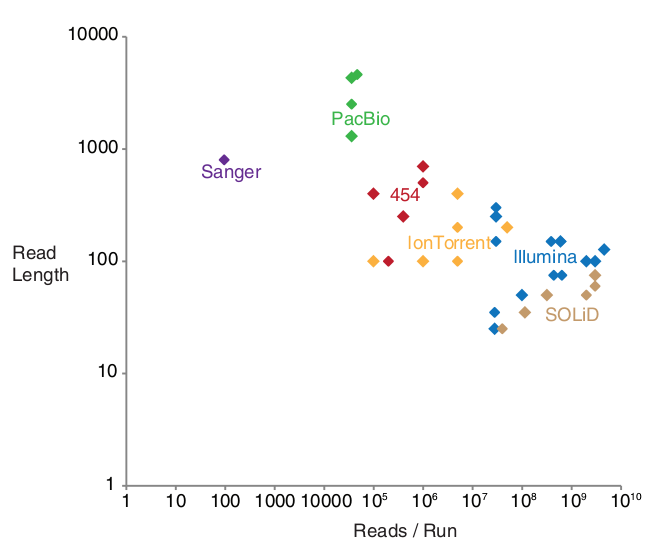
\includegraphics[scale=.55]{figure/read_per_run} 
  
  }
  
  \caption[Présentation de la taille des reads et du nombre de reads par run en fonction de la technologie de séquençage utilisée]{Présentation de la taille des reads et du nombre de reads par run en fonction de la technologie de séquençage utilisée d'après [@Hodkinson2015] : Chaque point représente une plateforme de séquençage, la couleur détermine la marque du séquenceur}\label{fig:readPerRun}
  \end{figure}
  
  \subsubsection{La capture des parties à séquencer, avantages et
  inconvénients}\label{la-capture-des-parties-a-sequencer-avantages-et-inconvenients}
  
  Pour de nombreuses applications, il peut être intéressant de ne
  séquencer qu'une partie du génome et non pas son intégralité. Dans cette
  sous partie de génome ciblé on peut trouver par exemple : une région
  génomique spécifique à laquelle une pathologie a déjà été associée,
  l'ensemble des exons de certains gènes candidats, ou encore
  l'intégralité des exons de l'ensemble des gènes codant pour une
  protéine. Dans ce dernier cas on parle alors de séquençage exomique ou
  \emph{whole exome sequencing} (WES). Les principaux avantages du WES par
  rapport au WGS sont son coût réduit ainsi qu'une masse de données moins
  importantes à stocker et à analyser. En effet, l'ensemble de l'exome ne
  représente qu'environ 1\% du génome entier. On considère cependant que
  ces parties codantes contiennent plus de 90\% des anomalies responsables
  de pathologies génétiques chez l'homme. Pour ces raisons, le WES est
  considéré comme le standard dans le cadre de recherche sur des
  pathologies génétiques et révèle être un outil puissant pour
  l'identification de variants associés à des pathologies (S. B. Ng et
  al., \protect\hyperlink{ref-Ng2010}{2010}). Le procédé de séquençage est
  identique au WGS, il est simplement précédé d'une étape d'enrichissement
  au cours de laquelle les exons sont capturés par hybridation à des
  sondes. De fait les exons capturés sont donc dépendants du kit de
  capture utilisé, cette technique permet donc de séquencer uniquement les
  exons connus et ciblés par les sondes. Il faut également noter que
  depuis quelques années, plusieurs études ont remis en cause l'intérêt du
  WES au profit du WGS, notamment car le WGS fournit une meilleure
  couverture sur l'exome que le WES (Lelieveld, Spielmann, Mundlos,
  Veltman, \& Gilissen, \protect\hyperlink{ref-Lelieveld2015}{2015},
  Meienberg, Bruggmann, Oexle, \& Matyas
  (\protect\hyperlink{ref-Meienberg2016}{2016})). De plus le WES montre
  une plus grande sensibilité au pourcentage de GC contenu dans la région
  à séquencer et à la sélection des kits de capture utilisés (Meienberg et
  al., \protect\hyperlink{ref-Meienberg2016}{2016}). Ainsi, bien que le
  WES soit encore à l'heure actuelle le choix privilégié dans la majorité
  des études, la réduction des coûts de séquençage et du stockage des
  données, pourraient permettre prochainement au WGS de remplacer
  totalement le WES ainsi que l'ensemble des techniques impliquant la
  capture de séquences ciblées (Meienberg et al.,
  \protect\hyperlink{ref-Meienberg2016}{2016}).
  
  \subsubsection{L'amplification}\label{lamplification}
  
  Dans la plupart des technologies, la phase de séquençage est précédée
  par une étape d'amplification de l'ADN. Cette amplification se fait dans
  la grande majorité des cas sur une surface solide exceptée pour la PCR
  en émulsion qui s'effectue en phase aqueuse. Elle permet d'obtenir dans
  une région définie plusieurs milliers de copies du même fragment d'ADN,
  appelés des clones. Cette étape assure que le signal émis lors du
  séquençage pourra être distingué du bruit. Chacun de ces \emph{spots}
  d'amplification appelés aussi centre de réaction, se retrouve donc être
  le représentant d'un unique fragment d'ADN. Ceux-ci seront ensuite
  séquencés parallèlement aux autres \emph{spots}. Une plateforme de
  séquençage peut gérer plusieurs millions de ces centres de réactions
  simultanément, séquençant ainsi plusieurs millions de molécules d'ADN en
  parallèle, donnant ainsi le nom de séquençage massif en parallèle à ces
  techniques. Cette étape d'amplification est généralement précédée d'une
  phase de fragmentation de l'ADN. Cette fragmentation peut être physique,
  enzymatique ou bien chimique. Ce sont les résidus d'ADN résultant de
  cette fragmentation qui seront ensuite amplifiés. Il existe quatre
  stratégies utilisées pour le clonage de l'ADN dans le cadre du NGS :
  
  \begin{enumerate}
  \def\labelenumi{\arabic{enumi}.}
  \tightlist
  \item
    \textbf{La PCR en émulsion ou emPCR} (\textbf{Figure :
    }\ref{fig:ngsampli} - \textbf{a}) : Le patron d'ADN fragmenté simple
    brin est lié à une séquence adaptatrice complémentaire et est capturé
    par une gouttelette aqueuse appelée micelle contenant une bille
    recouverte d'adaptateur complémentaire à celui fixé sur le fragment
    d'ADN ainsi que tous les composants nécessaires à la réaction de PCR.
    En respectant un ratio nombre de molécules d'ADN / nombre de billes,
    on va fixer un seul fragment d'ADN sur chaque bille. Chacune de ces
    billes seront donc, en fin de réaction, recouverte par plusieurs
    milliers de copies de la même séquence d'ADN.\\
  \item
    \textbf{L'amplification par pont sur face solide} (\textbf{Figure :
    }\ref{fig:ngsampli} - \textbf{b}) : Les fragments d'ADN sont liés à
    des séquences adaptatrices et lié par une de leurs extrémités à une
    amorce fixée sur un support solide. Du fait de la dilution, les
    molécules d'ADN se trouvent éloignées les unes des autres. L'extrémité
    libre du fragment interagit avec les amorces situées à proximité
    formant une structure en pont, d'où le nom de PCR en pont ou
    \emph{bridge-PCR}. La PCR va alors synthétiser un deuxième brin
    complémentaire aux fragments immobilisés sur le support. En procédant
    à des cycles de température comme pour une réaction PCR classique, on
    obtient à l'emplacement de chaque molécule d'ADN un massif de
    molécules fixé sur la plaque, toutes identiques à la molécule
    initiale.\\
  \item
    \textbf{Amplification par modèle mobile ou \emph{walking-template}
    }(\textbf{Figure : }\ref{fig:ngsampli} - \textbf{c}) : L'ADN fragmenté
    est lié à un adaptateur et lié à une amorce complémentaire fixée sur
    un support solide. Le brin complémentaire du fragment sera synthétisé
    par PCR à partir de l'amorce fixée. La molécule double brin
    nouvellement formée sera ensuite partiellement dénaturée permettant à
    l'extrémité libre de se fixer à une séquence amorce voisine. Des
    amorces \emph{reverse} sont ensuite utilisées pour resynthétiser un
    fragment d'ADN libre à partir des fragments fixés sur le support.\\
  \item
    (\textbf{Figure : }\ref{fig:ngsampli} - \textbf{d}) : \textbf{PAS DU
    TOUT COMPRIS LE MECHANISME !!! }
  \end{enumerate}
  
  \begin{figure}
  
  {\centering 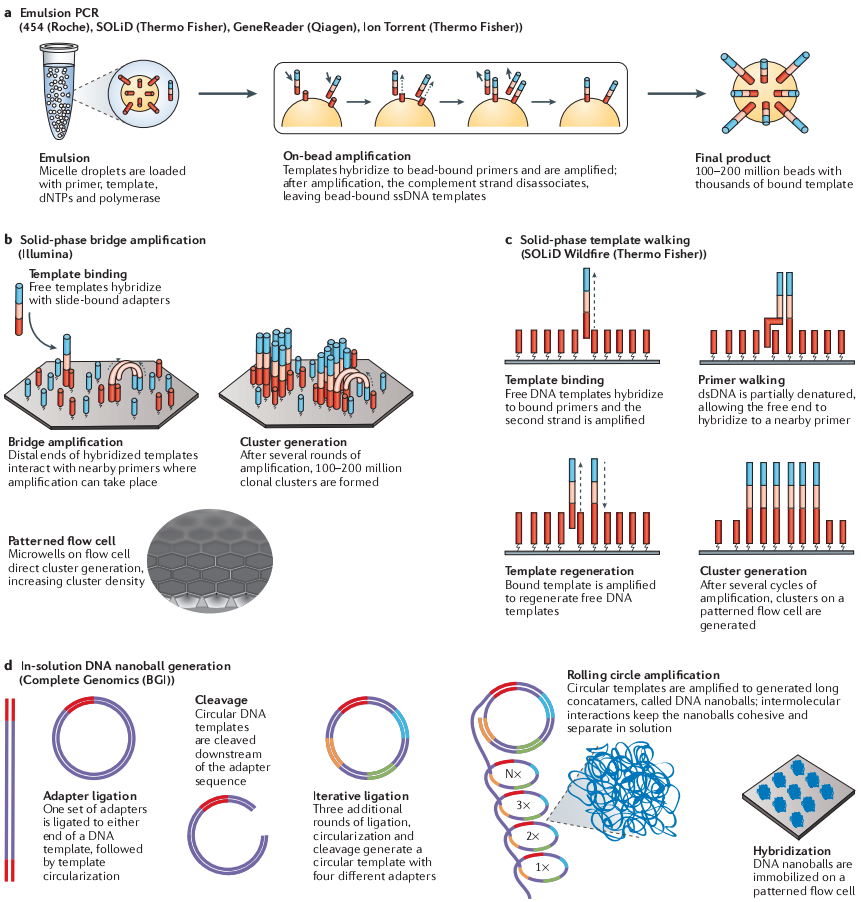
\includegraphics[scale=.455]{figure/ngs_amplification} 
  
  }
  
  \caption[Présentation des différentes stratégies d'amplification de l'ADN dans le cadre du NGS]{Présentation des différentes stratégies d'amplification de l'ADN dans le cadre du NGS d'après [@Goodwin2016] : **a** : PCR en émulsion. **b** : amplification par pont. **c** : Amplification par modèle mobile. **d** : }\label{fig:ngsampli}
  \end{figure}
  
  \newpage
  
  \subsubsection{La réaction de séquence}\label{la-reaction-de-sequence}
  
  La réaction de séquence est l'étape suivant l'amplification et consiste
  à déterminer l'ordre dans lequel se succèdent les nucléotides de
  l'ensemble des clones générés dans la phase d'amplification. Il existe
  deux technologies principales permettant le séquençage de \emph{reads}
  courts :\\
  
  \begin{enumerate}
  \def\labelenumi{\arabic{enumi}.}
  \tightlist
  \item
    \textbf{Séquençage par synthèse} (SBS) : Ce type de séquençage
    regroupe l'ensemble des méthodes utilisant l'ADN polymérase pour
    synthétiser de l'ADN. En 2016, Sahra Goodwin et ses collègues ont
    différentiés deux catégories de séquençage par synthèse (Goodwin,
    McPherson, \& McCombie, \protect\hyperlink{ref-Goodwin2016}{2016}) :
  
    \begin{enumerate}
    \def\labelenumii{\alph{enumii}.}
    \tightlist
    \item
      \textbf{Terminaison par cycle réversible}, \emph{cyclic reversible
      termination} (CRT) (\textbf{Figure : }\ref{fig:crtSeq}) : Cette
      méthode est caractérisée par l'utilisation de molécule dîtes
      terminatrices auxquelles le groupement \(\mathrm{3'-OH}\) est
      modifié de sorte à éviter l'élongation (J. Guo et al.,
      \protect\hyperlink{ref-Guo2008}{2008}), on parlera de groupement
      \(\mathrm{3'-bloqué}\). Une amorce liée au fragment d'ADN permettra
      l'initialisation du processus de polymérisation. À chaque cycle, un
      mix comprenant l'ensemble des quatre désoxynucléotides (dNTPs),
      préalablement labélisés par un fluorophore \(\mathrm{3'-bloqué}\),
      est mis en contact du fragment. Après l'incorporation d'un unique
      dNTP au fragment, les dNTPs non liés sont éliminés et la nature du
      dNTP ajouté est identifiée grâce à son fluorophore. Le fluorophore
      et le groupement \(\mathrm{3'-bloqué}\) sont retirés permettant
      ainsi à un nouveau cycle de commencer.
    \end{enumerate}
  \end{enumerate}
  
  \begin{figure}
  
  {\centering 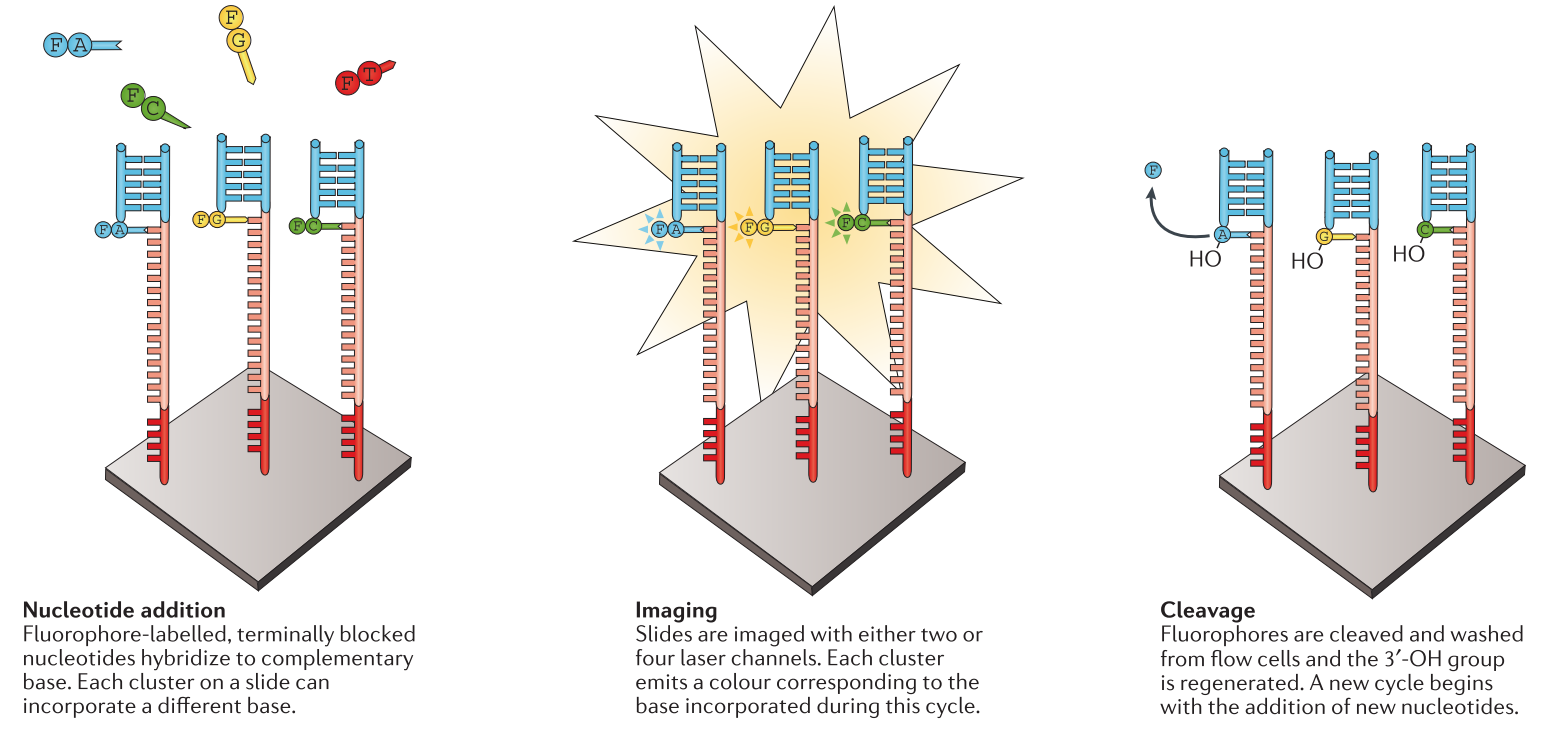
\includegraphics[scale=.24]{figure/CRT_seq_illumina} 
  
  }
  
  \caption[Séquençage CRT tel qu'il est effectué par Illumina]{Séquençage CRT tel qu'il est effectué par Illumina d'après [@Goodwin2016] : **a** : Ajout d'un dNTP labellisé par un fluorophore 3'-bloqué. **b** : Identification du dNTP ajouté grâce au fluorophore. **c** : Le fluorophore est clivé du dNTP et le groupement 3'-OH est reformé à partir du groupement 3'-bloqué permettant ainsi l'élongation}\label{fig:crtSeq}
  \end{figure}
  
  \newpage
  
  \begin{enumerate}
  \def\labelenumi{\alph{enumi}.}
  \setcounter{enumi}{1}
  \tightlist
  \item
    \textbf{Addition de nucléotide unique}, \emph{single nucleotide
    addition} (SNA) (\textbf{Figure : }\ref{fig:snaSeq}) :
    L'initialisation de la méthode SNA est identique à celle de la méthode
    CRT. La différence se fait donc au moment de la phase d'élongation.
    Contrairement à la méthode CRT, le mix contenant les dNTPs ne contient
    qu'un seul type de dNTP. Quatre mixs différents sont donc présentés
    successivement au fragment d'ADN à séquencer, ceux-ci se fixeront
    uniquement s'ils sont complémentaires à la séquence. Ces dNTPs n'ont
    donc pas besoin d'être \(\mathrm{3'-bloqué}\) puisqu'un seul dNTP est
    ajouté à chaque itération. Après avoir présenté un mix, on vérifie si
    un dNTP s'est lié au fragment. Lors des séquences homopolymériques
    (plusieurs nucléotides identiques successifs dans la séquence),
    plusieurs dNTPs sont donc liés simultanément, cela sera détecté car le
    signal émis est proportionnel au nombre de nucléotides ajoutés.
  \end{enumerate}
  
  \begin{figure}
  
  {\centering 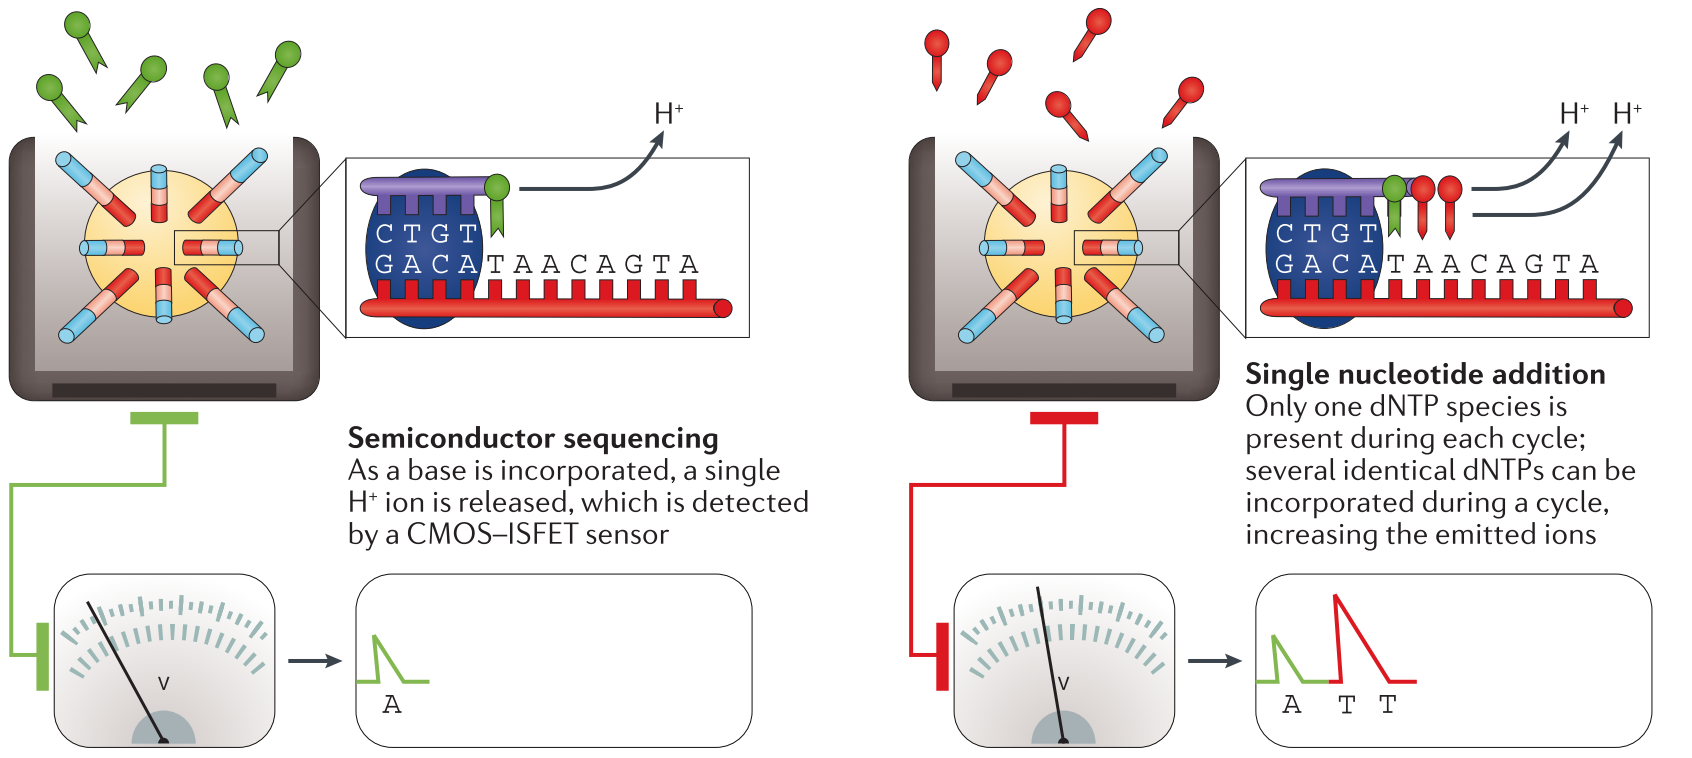
\includegraphics[scale=.26]{figure/SNA_seq_ionTorrent} 
  
  }
  
  \caption[Séquençage SNA tel qu'il est effectué par Ion Torrent]{Séquençage SNA tel qu'il est effectué par Ion Torrent d'après [@Goodwin2016] : **a** : Mise en présence du patron d'ADN à séquencer avec un mix contenant un seul type de dNTP, si le dNTP est complémentaire au patron, il se fixe et libère un proton permettant d'identifier la liaison. **b** : Dans le cas d'homopolymère, autant de proton sont relâchés de bases constituant l'homopolymère, le signal émit est donc plus fort permettant d'identifier le nombre des dNTPs liés}\label{fig:snaSeq}
  \end{figure}
  
  \newpage
  
  \begin{enumerate}
  \def\labelenumi{\arabic{enumi}.}
  \setcounter{enumi}{1}
  \tightlist
  \item
    \textbf{Séquençage par ligation} (SBL) : Par définition, cette méthode
    est basée sur l'hybridation et la ligation de l'ADN à une sonde liée à
    un fluorophore (Tomkinson, Vijayakumar, Pascal, \& Ellenberger,
    \protect\hyperlink{ref-Tomkinson2006}{2006}). Ce processus utilise les
    caractéristiques de la ligase, une enzyme qui a pour fonction de
    catalyser la liaison de deux brins d'ADN par des liaisons
    phosphodiester. La sonde est constituée d'une ou deux bases connues,
    on parle alors de \emph{one-base-encoded probes} ou de
    \emph{two-bases-encoded probes} suivis d'une succession de bases
    ``dégénérées'' ou universelle, c'est à dire, des bases capables de
    s'apparier avec n'importe laquelle des quatre bases de l'ADN.
  \end{enumerate}
  
  \begin{figure}
  
  {\centering 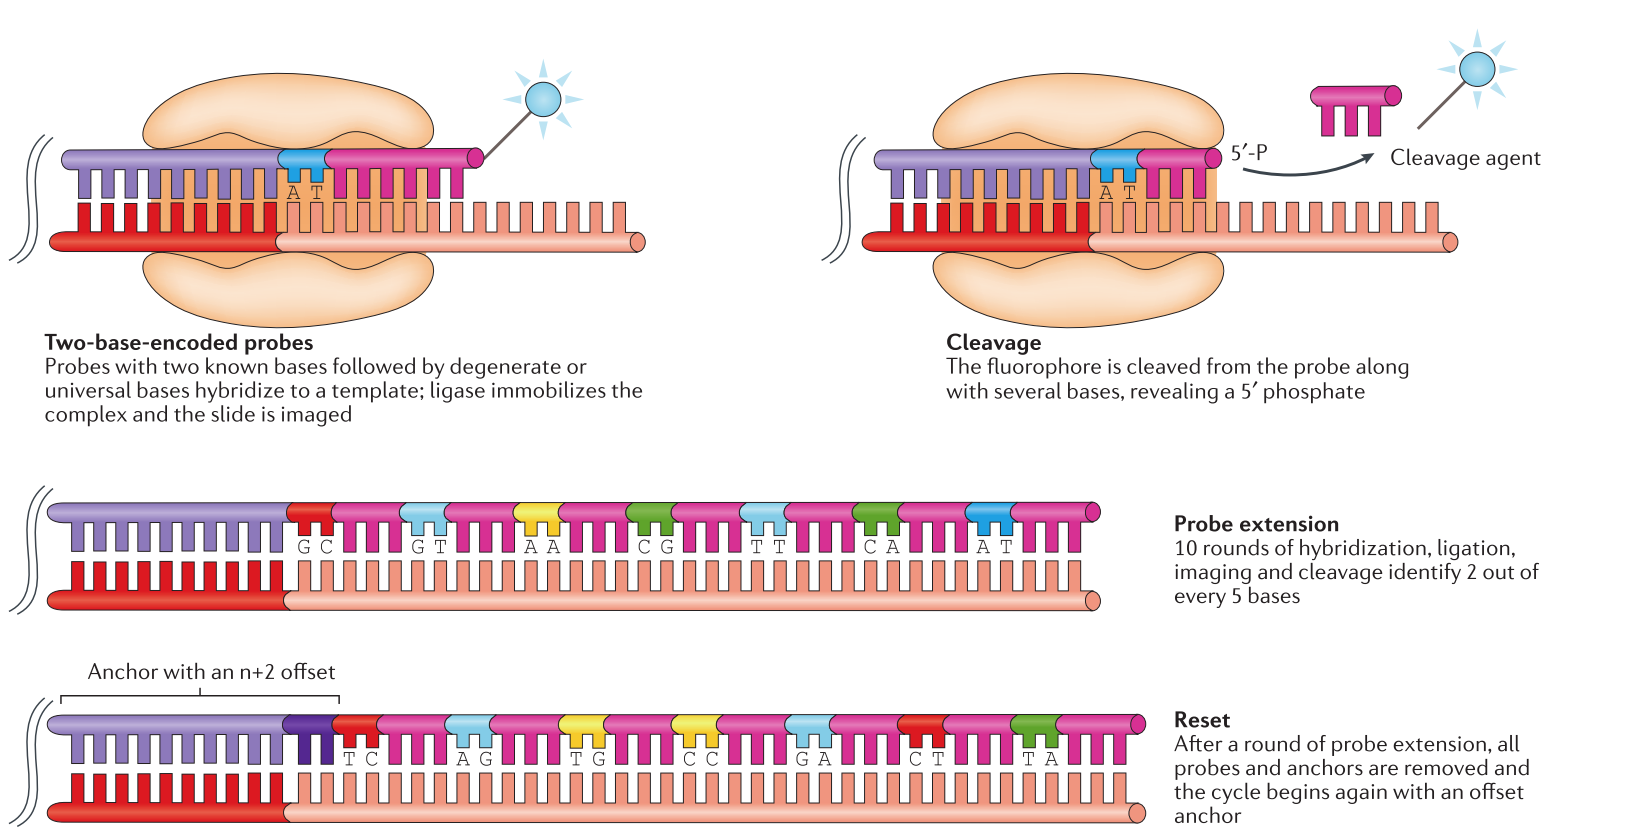
\includegraphics[scale=.26]{figure/SBL_seq_solid} 
  
  }
  
  \caption[Séquençage SBL tel qu'il est effectué par SOLiD]{Séquençage SBL tel qu'il est effectué par SOLiD d'après [@Goodwin2016] : }\label{fig:sblSeq}
  \end{figure}
  
  \newpage  
  
  \section{L'analyse bioinformatique des données de
  NGS}\label{lanalyse-bioinformatique-des-donnees-de-ngs}
  
  La stratégie consistant à séquencer en parallèle plusieurs milliers de
  \emph{reads} courts a engendré plusieurs nouveaux défis bioinformatique
  dans l'analyse et l'interprétation des données de séquençage et la
  recherche de variants dans le génome humain (Wold \& Myers,
  \protect\hyperlink{ref-Wold2007}{2007}, M. Q. Yang et al.
  (\protect\hyperlink{ref-Yang2009}{2009})). Ces techniques ont été
  appliquées dans différents contextes, notamment la métagénomique (J. Qin
  et al., \protect\hyperlink{ref-Qin2010}{2010}), la détection de SNPs
  (Van Tassell et al., \protect\hyperlink{ref-VanTassell2008}{2008}) et de
  variants structuraux (Alkan et al.,
  \protect\hyperlink{ref-Alkan2010}{2010}, Medvedev, Stanciu, \& Brudno
  (\protect\hyperlink{ref-Medvedev2009}{2009})) mais également dans des
  études portant sur la méthylation de l'ADN (K. H. Taylor et al.,
  \protect\hyperlink{ref-Taylor2007}{2007}), l'analyse de l'expression des
  ARNs messagers (Sultan et al.,
  \protect\hyperlink{ref-Sultan2008}{2008}), dans la génétique du cancer
  (Guffanti et al., \protect\hyperlink{ref-Guffanti2009}{2009}) et la
  médecine personnalisée (Auffray, Chen, \& Hood,
  \protect\hyperlink{ref-Auffray2009}{2009}). Cependant, pour l'ensemble
  de ces applications, la grande quantité de données générées par chaque
  analyse pose plusieurs défis informatiques (Horner et al.,
  \protect\hyperlink{ref-Horner2009}{2009}). En effet, les progrès
  techniques des dernières décennies ont rendu possible le séquençage de
  plusieurs millions des \emph{reads} d'ADN en un temps relativement court
  et à coûts raisonnable. Ainsi, l'émergence du séquençage haut débit et
  notamment du WGS et du WES a permis de réunir une quantité jusqu'à
  présent inégalée d'informations sur les variations génétiques, et sur
  les gènes et leurs fonctions (E. R. Mardis,
  \protect\hyperlink{ref-Mardis2008}{2008}, Bentley
  (\protect\hyperlink{ref-Bentley2006}{2006})). Cependant, de par leur
  nature et leur quantité, l'acquisition de ces nouvelles données a
  engendrée de nouvelles problématiques qui freinent les biologistes dans
  leurs recherches.
  
  \subsection{Les données fournies par le
  NGS}\label{les-donnees-fournies-par-le-ngs}
  
  \subsubsection{\texorpdfstring{Un \emph{read} c'est quoi
  ?}{Un read c'est quoi ?}}\label{un-read-cest-quoi}
  
  Après la phase d'amplification, chaque clone est analysé puis, la
  séquence composant chacun de ce clone est déterminée. La taille de cette
  séquence varie en fonction des plateformes de séquençage mais est
  généralement comprise entre 40 et 150 pb pour le NGS (\textbf{Figure :
  }\ref{fig:readPerRun}). Depuis quelques années, un nouveau type de
  \emph{read} est apparu, le \emph{read} \emph{paired-end}. Contrairement
  au \emph{reads} classiques (single-end), les deux extrémités (les
  \emph{ends}) du fragment d'ADN sont désormais séquencées. La distance
  séparant les deux extrémités du \emph{read} étant connue, cela permet
  aux aligneurs d'utiliser cette information afin d'améliorer leur
  précision, notamment dans les zones répétées (H. Li et al.,
  \protect\hyperlink{ref-Li2008}{2008}). En plus de SNP, ce format permet
  de mettre en évidence des variants structuraux (Korbel et al.,
  \protect\hyperlink{ref-Korbel2009}{2009}).
  
  \newpage
  
  \subsubsection{Le format FASTQ}\label{fastq}
  
  Le format FASTQ (\textbf{Figure : }\ref{fig:fastqformat}) est
  actuellement le format de donnée le plus couramment utilisé dans le
  cadre du séquençage haut-débit. Sa création est cependant antérieure à
  l'émergence du NGS puisqu'il fut inventé à la fin du XX\(^{ième}\) par
  Jim Mullikin au
  \href{https://fr.wikipedia.org/wiki/Wellcome_Trust_Sanger_Institute}{Wellcome
  Trust Sanger Institute} alors que le séquençage commençait à prendre de
  l'ampleur grâce à des projets tels que le
  \href{https://fr.wikipedia.org/wiki/Projet_G\%C3\%A9nome_Humain}{Projet
  Génome Humain}. La quantité de données générées par ces programmes a
  nécessité une analyse automatisée, c'est ainsi que chaque base séquencée
  s'est vue associer un score de qualité appelé \emph{Phred-score}. Chaque
  séquence générait ainsi deux fichiers, un fichier FASTA contenant les
  séquences et un fichier QUAL contenant les scores \emph{Phred} associés
  à chaque base du fichier FASTA Cock2009. Plus tard, afin de n'avoir à
  manipuler qu'un seul fichier, les fichiers FASTA et QUAL furent
  fusionnés en ce que l'on appelle désormais le fichier FASTQ. Ce format
  est aujourd'hui le plus utilisé par les différents séquenceurs on peut
  cependant noter certaines différences dans les formats FASTQ provenant
  des différentes plateformes puisqu'à l'époque, aucune spécification
  officielle n'avait été donnée (Cock, Fields, Goto, Heuer, \& Rice,
  \protect\hyperlink{ref-Cock2009}{2009}).
  
  \begin{figure}
  
  {\centering 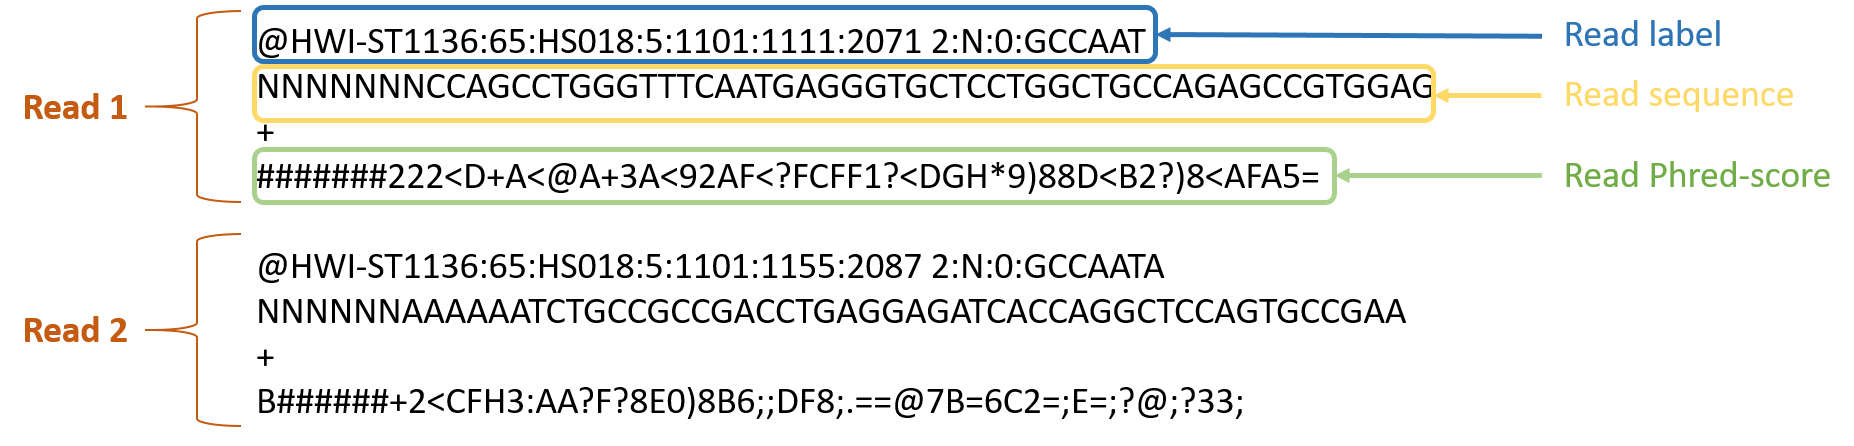
\includegraphics[scale=.55]{figure/fastq} 
  
  }
  
  \caption[présentation d'un fichier FASTQ (FIGURE A CHANGER)]{présentation d'un fichier FASTQ (FIGURE A CHANGER) : **a** : identifiant du *read*. **b** : séquence du *read*. **c** : score de qualité associé}\label{fig:fastqformat}
  \end{figure}
  
  \newpage
  
  \hypertarget{lalignement}{\subsection{L'alignement}\label{lalignement}}
  
  L'alignement constitue la première étape de l'analyse des données de NGS
  lorsqu'un génome de référence est disponible. L'objectif de l'alignement
  est de déterminer la position correcte de chacun des \emph{reads}
  séquencés le long du génome de référence. Cette référence est souvent
  construite à partir des données de séquençage de plusieurs donneurs et
  ne représente donc pas la séquence d'un individu en particulier mais est
  censé représenter la séquence consensus d'une espèce donnée. Par
  exemple, la séquence de référence humaine GRCh37 (\emph{Genome Reference
  Consortium human build 37}) a été créé à partir de 13 volontaires
  anonymes New-Yorkais. Dès lors, cette référence servira de patron aux
  aligneurs afin qu'ils replacent correctement les différents \emph{reads}
  des individus séquencés. Cette étape peut être comparée à la
  reconstruction d'un puzzle dans laquelle les \emph{reads} seraient les
  pièces et le génome de référence le modèle. Elle constitue probablement
  l'étape la plus importante de l'analyse des données issues du séquençage
  haut débit (Flicek \& Birney, \protect\hyperlink{ref-Flicek2009}{2009})
  car elle est la base sur laquelle repose l'ensemble des étapes
  effectuées en aval, notamment l'appel des variants (R. Nielsen, Paul,
  Albrechtsen, \& Song, \protect\hyperlink{ref-Nielsen2011}{2011}).
  Cependant, l'étape d'alignement est sujette à de nombreuses erreurs dont
  certaines proviennent directement des erreurs survenues lors de l'étape
  de séquençage, d'autres, sont dues aux caractéristiques des régions
  séquencées comme par exemple les séquences répétées (Ben Langmead \&
  Salzberg, \protect\hyperlink{ref-Langmead2012}{2012}) qui pourront
  entraîner l'alignement d'un même \emph{read} à plusieurs régions du
  génome (Treangen \& Salzberg,
  \protect\hyperlink{ref-Treangen2013}{2013}). De nombreux aligneurs ont
  émergés afin de répondre au mieux à cette problématique tel que Bowtie
  (B Langmead, Trapnell, Pop, \& Salzberg,
  \protect\hyperlink{ref-Langmead2009}{2009}), Bowtie2 (Ben Langmead \&
  Salzberg, \protect\hyperlink{ref-Langmead2012}{2012}), BWA, NovoAlign,
  MAGIC (Su et al., \protect\hyperlink{ref-Su2014}{2014}). De nombreuses
  études ont cependant montrées de grandes différences entre ces
  aligneurs, au niveau du temps de calcul, de leur coût en mémoire et de
  leur taux d'erreur (Ruffalo, Laframboise, \& Koyutürk,
  \protect\hyperlink{ref-Ruffalo2011}{2011}, Thankaswamy-Kosalai, Sen, \&
  Nookaew (\protect\hyperlink{ref-Thankaswamy-Kosalai2017}{2017}), S. Bao
  et al. (\protect\hyperlink{ref-Bao2011}{2011})).
  
  \newpage
  
  \hypertarget{varcall}{\subsection{L'appel des variants}\label{varcall}}
  
  L'appel des variants, ou \emph{variant calling}, fait référence à
  l'ensemble des méthodes permettant d'identifier des SNVs ou des indels à
  partir des résultats de l'alignement. Cette étape est souvent
  différenciée de l'alignement, cependant, les résultats de l'appel étant
  extrêmement dépendants de l'alignement, il est conseillé d'effectuer son
  appel en tenant compte de l'aligneur choisi (R. Nielsen et al.,
  \protect\hyperlink{ref-Nielsen2011}{2011}, M. A. DePristo et al.
  (\protect\hyperlink{ref-DePristo2011}{2011}), Lunter \& Goodson
  (\protect\hyperlink{ref-Lunter2011}{2011})). On appellera variant toute
  différence de séquence observée entre un individu et la séquence de
  référence utilisée. Pour reprendre la comparaison avec la construction
  d'un puzzle, cette étape consiste à détecter quelles sont les pièces qui
  présentent des différences avec le modèle. De nombreux logiciels
  d'appels des variants, ou \emph{caller}, basés sur des algorithmes
  différents ont émergés ces dernières années pour répondre à cette
  problématique. Parmi les plus connus on note SAMtools (H. Li et al.,
  \protect\hyperlink{ref-Li2009}{2009}), Genome Analysis Tool Kit -
  HaplotypeCaller (GATK-HC) (McKenna et al.,
  \protect\hyperlink{ref-McKenna2010}{2010}), Freebayes, SOAPindel et TVC.
  Les quatre premiers cités, peuvent être utilisés pour analyser des
  données provenant de tout type de plateforme de séquençage contrairement
  à TVC qui a été développé spécifiquement pour les données provenant de
  Ion Proton. Les données issues de NGS peuvent présenter un taux d'erreur
  important. Ce taux d'erreur est multifactoriel et inclus notamment les
  erreurs de l'alignement. L'un des éléments clef à prendre en compte pour
  pouvoir effectuer un appel de qualité est la couverture de la position
  appelée (D. Sims et al., \protect\hyperlink{ref-Sims2014}{2014}).
  Cependant, malgré la prise en compte de cet élément, l'appel de variants
  reste un processus difficile souvent lié à plusieurs erreurs. Plusieurs
  de ces erreurs sont même directement liées à la plateforme de séquençage
  utilisée en amont, et les différents logiciels ne présentent pas les
  mêmes performances en fonction de ces différentes plateforme (S. Hwang,
  Kim, Lee, \& Marcotte, \protect\hyperlink{ref-Hwang2015}{2015}), c'est
  pourquoi il convient d'adapter le logiciel d'appel en fonction de la
  plateforme de séquençage utilisée préalablement. Les erreurs d'appel
  sont généralement classées en trois catégories et certains aligneurs
  auront tendance à être plus sujets à l'un de ces types d'erreur qu'à
  l'autre (\textbf{Figure : }\ref{fig:snperror}) :
  
  \begin{enumerate}
  \def\labelenumi{\arabic{enumi}.}
  \tightlist
  \item
    Oubli de l'allèle de référence (\textbf{IR}, \emph{ignore the
    reference allele}) : représente un variant appelé homozygote
    correspondant en réalité à un variant hétérozygote composé de l'allèle
    de référence et d'un allèle variant.\\
  \item
    Ajout de l'allèle de référence (\textbf{AR}, \emph{adding the
    reference allele}) : représente un variant appelé hétérozygote composé
    de l'allèle de référence et d'un allèle variant correspondant en
    réalité à un variant homozygote composé de deux allèles variants.\\
  \item
    Autres : incluent l'ensemble des autres types d'appel erronés
    indépendamment de l'allèle de référence
  \end{enumerate}
  
  \newpage
  
  \begin{figure}
  
  {\centering 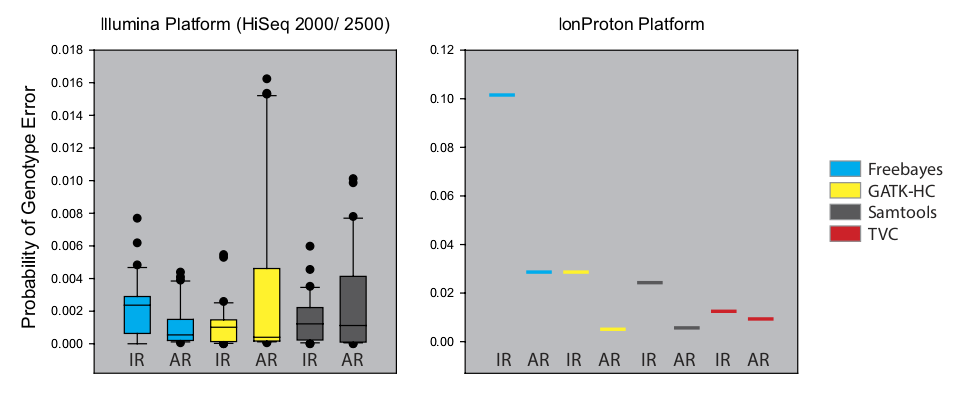
\includegraphics[scale=.50]{figure/snp_error_type} 
  
  }
  
  \caption[Représentation des erreurs d'appel de type IR et AR en fonction de la plateforme de séquençage et du logiciel d'appel]{Représentation des erreurs d'appel de type IR et AR en fonction de la plateforme de séquençage et du logiciel d'appel d'après [@Hwang2015] : Pour la plateforme Illumina, on peut voir que Freebayes favorise les appels variant-homozygote tandis que GATK-HC et Samtools favorisent les appels hétérozygotes. Pour la plateforme Ion Proton, les 4 logiciels entraînent des erreurs de type IR}\label{fig:snperror}
  \end{figure}
  
  De même que pour l'aligneur, le choix du logiciel d'appel est crucial
  car il existe de nombreuses différences dans les variants appelés par
  différents logiciels se basant sur les mêmes données brutes (Baes et
  al., \protect\hyperlink{ref-Baes2014}{2014}, O'Rawe et al.
  (\protect\hyperlink{ref-ORawe2013}{2013}), J. A. Rosenfeld, Mason,
  Smith, Wallin, \& Diekhans
  (\protect\hyperlink{ref-Rosenfeld2012}{2012})). En effet, en 2013, une
  étude comparant les résultats de 5 \emph{callers} montraient que
  seulement 57,4\% des variants étaient appelés par les 5 \emph{callers}
  et que 80,7\% des variants étaient appelés par au moins 3 d'entre eux.
  Ce taux chutait drastiquement pour les indels puisque la concordance
  était cette fois seulement de 26,8\% pour les indels non retrouvés par
  les 3 \emph{callers} (O'Rawe et al.,
  \protect\hyperlink{ref-ORawe2013}{2013}). Ces résultats sont cependant à
  pondérer avec une étude de 2015 comparant 4 \emph{callers} et montrant
  que 91,7\% des SNVs séquencés sur une plateforme Illumina étaient
  appelés par 3 \emph{callers}, cependant, pour les variants séquencés sur
  Ion Proton, seulement 27,3\% des variants étaient appelés par au moins 3
  \emph{callers} et 57,4\% des variants n'étaient appelés que par un seul
  des \emph{callers} (S. Hwang et al.,
  \protect\hyperlink{ref-Hwang2015}{2015}).
  
  \newpage
  
  \subsection{L'annotation des variants, filtrage et
  priorisation}\label{lannotation-des-variants-filtrage-et-priorisation}
  
  Traditionnellement, les scientifiques et les laboratoires dans lesquels
  ils travaillaient développaient leur expertise dans un nombre de
  pathologies et de gènes associés limité. L'émergence du NGS est en train
  de remettre en cause cette pratique car la totalité de l'exome ou du
  génome peut permettre de couvrir tous les gènes quelque en une seule et
  même analyse. De nombreux praticiens maintiennent cependant une
  spécialisation pour certains groupes de pathologies qui est précieuse
  pour l'analyse des données et l'obtention d'un diagnostic. En effet il
  est courant de retrouver entre 20.000 et 25.000 variants différents par
  exome (Gonzaga-Jauregui, Lupski, \& Gibbs,
  \protect\hyperlink{ref-Gonzaga-Jauregui2012}{2012}). Afin de pouvoir
  lier un variant à une pathologie, il est indispensable d'annoter cet
  ensemble de variants, c'est à dire d'associer à ces variants l'ensemble
  des informations qui les caractérisent afin de pouvoir les replacer dans
  leur contexte biologique. Ces informations serviront ensuite
  d'indicateur afin filtrer ou prioriser un variant. Cette dernière étape
  de l'analyse est elle aussi cruciale puisqu'elle permet de réduire le
  nombre de variants à considérer. On peut généralement distinguer deux
  niveaux d'annotations d'un variant :
  
  \begin{enumerate}
  \def\labelenumi{\arabic{enumi}.}
  \tightlist
  \item
    \textbf{Au niveau du variant} : Ce niveau d'annotation regroupe
    l'ensemble des informations \textbf{spécifiques} à un variant
  
    \begin{enumerate}
    \def\labelenumii{\alph{enumii}.}
    \tightlist
    \item
      \textbf{Informations issues des résultats du séquençage} : la
      couverture du variant ainsi que la qualité qui lui est associée
      peuvent permettre de considérer un variant comme étant fiable ou
      non. Le génotype associé à ce variant est également une information
      importante.\\
    \item
      \textbf{La fréquence du variant dans la population générale} :
      l'émergence du séquençage haut-débit a permis de de gros consortium
      tel que ESP6500 (\href{http://evs.gs.washington.edu/EVS/}{Exome
      Variant Server, NHLBI GO Exome Sequencing Project (ESP), Seattle,
      WA}), 1KG (1000 Genomes Project Consortium et al.,
      \protect\hyperlink{ref-1000GenomesProjectConsortium2015}{2015}). Ces
      consortiums ont pu mettre à disposition du public de données de
      séquençage exomique de 6503 individus pour ESP et de 2504 pour la
      phase 3 du 1000Genomes. On peut également noter l'\emph{Exome
      Aggregate Consortium} (ExAC) (Lek et al.,
      \protect\hyperlink{ref-Lek2016}{2016}) qui n'a effectué aucun
      séquençage mais qui a regroupé les données de plusieurs gros jeux
      (notamment 1000Genome et ESP) afin de leur appliquer la même analyse
      bioinformatique harmonisant ainsi les données provenant de 60.706
      individus non apparentés. Cette masse d'information permet de se
      faire une idée de la fréquence d'un variant dans la population
      générale et même au sein de sous population humaine. On considère
      qu'un variant fréquent ne peut pas être délétère, sinon il aurait
      été contre-sélectionné au cours de l'évolution.
    \end{enumerate}
  \end{enumerate}
  
  \newpage
  
  \begin{enumerate}
  \def\labelenumi{\alph{enumi}.}
  \setcounter{enumi}{2}
  \tightlist
  \item
    \textbf{Son impact sur le transcrit} : Dans la plupart des analyses
    phénotype-génotype, les chercheurs se limitent aux variants
    chevauchant des transcrits codants pour une protéine. Il est donc
    important de savoir l'impact d'un variant sur ce transcrit, c'est à
    dire si le variant va causer une mutation synonyme, un faux-sens ou
    une mutation tronquante. Des logiciels tel que \emph{Variant Effect
    Predictor} (VEP) (W. McLaren et al.,
    \protect\hyperlink{ref-McLaren2016}{2016}), SnpEff (Cingolani et al.,
    \protect\hyperlink{ref-Cingolani2012}{2012}) ou encore ANNOVAR (K.
    Wang, Li, \& Hakonarson, \protect\hyperlink{ref-Wang2010}{2010}) vont
    prédire l'impact qu'aura un variant sur les différents transcrits
    qu'il chevauche. D'autres logiciels tel que SIFT (P. Kumar, Henikoff,
    \& Ng, \protect\hyperlink{ref-Kumar2009}{2009}), PROVEAN (Y. Choi,
    Sims, Murphy, Miller, \& Chan,
    \protect\hyperlink{ref-Choi2012}{2012}), Polyphen2, ou encore CADD
    vont eux chercher à prédire la pathogénicité de ce variant, c'est à
    dire la probabilité que ce variant soit délétère pour la fonction de
    la protéine. Bien que cette information soit important, elle est à
    pondérer étant donné le peu de concordance qu'il existe entre les
    prédictions de ces différents logiciel (\textbf{Figure :}
    \ref{fig:vennpred}).
  \end{enumerate}
  
  \begin{figure}
  
  {\centering 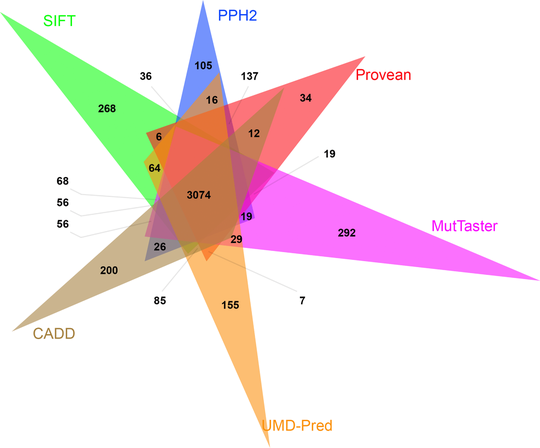
\includegraphics[scale=.7]{figure/venn_Diag_patho_pred} 
  
  }
  
  \caption[Diagramme de Venn des prédictions de pathogénicités de six logiciels]{Diagramme de Venn des prédictions de pathogénicités de six logiciels d'après [@Salgado2016] : }\label{fig:vennpred}
  \end{figure}
  
  \newpage
  
  \begin{enumerate}
  \def\labelenumi{\arabic{enumi}.}
  \setcounter{enumi}{1}
  \tightlist
  \item
    \textbf{Au niveau de l'unité génétique} : DÉCRIRE UNITÉ GÉNÉTIQUE
    (gène, transcrit). L'annotation au niveau de l'unité génétique
    consiste à récupérer l'ensemble des informations disponible non plus
    sur le variant uniquement mais sur la ou les unités génétiques qu'il
    impacte. Ce ``dézoom'' permet d'ajouter des informations
    complémentaires particulièrement utiles notamment lorsque peu
    d'informations sont disponibles sur le variant lui-même. En pratique,
    la plupart des variants connus pour impliquer une pathologie sont des
    variants privés, c'est à dire spécifiques à une famille ou un individu
    limitant ainsi la quantité d'information disponible sur ce variant.
    Élargir l'annotation au niveau des unités génétiques impactés par des
    variants permet d'augmenter considérablement la quantité d'information
    disponible et permet donc d'améliorer la capacité des algorithmes à
    filtrer et / ou prioriser les variants rendant donc les analyses plus
    efficaces. On peut relever certains logiciels tel que le \emph{Protein
    ANalysis THrough Evolutionary Relationships} (PANTHER) (Mi et al.,
    \protect\hyperlink{ref-Mi2017}{2017}) qui permet par exemple de
    classer une liste de gènes en fonction de leurs fonctions
    moléculaires, des processus biologiques et des voies de signalisation
    dans lesquels ils sont impliqués. On peut également noter \emph{the
    Human Phenotype Ontology project} (HPO) (Köhler et al.,
    \protect\hyperlink{ref-Kohler2014}{2014}) qui fournit une
    classification (À compléter). Plus récemment, on a pu voir émerger des
    ``scores mutationnel'' tel que RVIS (Petrovski et al.,
    \protect\hyperlink{ref-Petrovski2013}{2013}) ou encore le pLI (Lek et
    al., \protect\hyperlink{ref-Lek2016}{2016}). En se basant sur les
    bases de données telle que ESP ou encore ExAC, ces scores permettent
    de classer les gènes en fonction de leur tolérance (ou intolérance)
    aux variations avec l'idée sous-jacente que ``les gènes impliqués dans
    des pathologies à transmission Mendéliennes'' devraient être moins
    tolérant aux variations que les autres.
  \end{enumerate}
  
  Comme nous l'avons vu, le développement d'outils permettant l'analyse
  des données NGS est extrêmement important puisqu'il permet aux
  biologistes de faire face à la masse de données générés par le
  séquençage haute débit l'aidant ainsi dans ses prises de décisions. Il
  est à noter que la plupart de ces données filtrées sont extrêmement
  dépendantes du jeu de gènes utilisés, les prédictions seront donc
  différentes si l'on se base sur les gènes RefSeq, Ensembl ou UCSC (D. J.
  McCarthy et al., \protect\hyperlink{ref-McCarthy2014}{2014},S. Zhao \&
  Zhang (\protect\hyperlink{ref-Zhao2015}{2015})) bien que les gènes du
  \emph{Consensus Coding Sequence project} (CCDS) soient bien représentés
  par ces trois listes (K. D. Pruitt et al.,
  \protect\hyperlink{ref-Pruitt2009}{2009}). De même, pour une même liste
  de gêne, de nombreuses différences seront observées en fonction du ou
  des logiciels de prédiction utilisés (D. J. McCarthy et al.,
  \protect\hyperlink{ref-McCarthy2014}{2014}, Salgado, Bellgard,
  Desvignes, \& B??roud (\protect\hyperlink{ref-Salgado2016}{2016})).
  
  \newpage
  
  \subsection{Conclusion NGS}\label{conclusion-ngs}
  
  En moins de 10 ans, les technologies NGS sont passées du séquençage de
  panels de gènes (environ 100 Mb pour le Roche GS FLX system) au
  séquençage de génomes entiers (environs 1500 GB pour l'Illumina Hiseq
  4000) et d'une utilisation exclusive à la recherche à l'analyse en
  routine dans un cadre de diagnostics cliniques. Le nombre croissant
  d'études utilisant le WGS ou le WES démontre le pouvoir de ces approches
  dans des analyses phénotypes-génotypes impliquant des pathologies à
  transmission Mendélienne. De plus, la diminution constante des coûts par
  génomes / exomes séquencés laisse supposer que ces technologies
  deviendront d'ici peut le fer de lance de la génétique clinique moderne.
  Cependant, cette quantité de données produites crées de nouvelles
  problématiques pour les généticiens qui se retrouvent désormais face au
  ``déluge de données génétiques'' (Schatz \& Langmead,
  \protect\hyperlink{ref-Schatz2013}{2013}). Le succès d'une étude n'étant
  plus lié aux capacités de séquençage mais aux compétences dans l'analyse
  et l'interprétation des données produites. Bien que de nombreux efforts
  soient faits pour palier la contrainte instaurée par les \emph{reads}
  courts dans le cadre d'analyse génomique, les solutions informatiques et
  bioinformatiques proposées jusqu'à présent restent en dessous des
  besoins créés par NGS (J. D. McPherson,
  \protect\hyperlink{ref-McPherson2009}{2009}). Cette masse de données
  produite, à l'origine du succès du séquençage haut-débit dans le domaine
  de la génomique et de la post-génomique, se trouve désormais être un
  frein à la compréhension et l'interprétation des réseaux de gènes et
  leurs implications dans des pathologies. La limitation de cette
  technologie n'est donc plus le séquençage d'un, de plusieurs, ou de
  l'ensemble des gènes, mais plutôt l'analyse et l'interprétation des
  donnée générée. Le processus allant de l'extraction de l'ADN à
  l'identification d'un variant responsable d'une pathologie comprend de
  nombreuses étapes apportant avec elles leur lot d'erreurs. Bien que dans
  chacune de ces phases, de nombreux acteurs soient en concurrence et
  cherchent à atteindre une solution idéale, celle-ci n'a toujours pas été
  trouvée et la prolifération des logiciels et algorithmes d'analyses,
  bien que nécessaire, peut également parfois augmenter la confusion.
  
  Malgré les dizaines de milliers d'exomes et de génomes ayant été jusqu'à
  présent étudiés, notre compréhension des mécanismes moléculaires qui
  sous-tendent la variété génomique humaine reste limitée, et ce
  particulièrement dans le contexte de l'analyse de pathologies
  génétiques. En effet, à l'heure actuelle, plus de 3700 pathologie à
  transmission Mendélienne ont été caractérisées mais un nombre similaire
  ont toujours une cause inconnue (Amberger, Bocchini, \& Hamosh,
  \protect\hyperlink{ref-Amberger2011}{2011}). L'élucidation de ces
  mystères passera probablement par une harmonisation des méthodes de
  production des données ainsi que par l'amélioration des techniques
  d'analyses.
  
  \chapter{Mise en place d'une stratégie pour l'analyse des données
  exomiques -- application en recherche
  clinique}\label{mise-en-place-dune-strategie-pour-lanalyse-des-donnees-exomiques-application-en-recherche-clinique}
  
  \newpage
  
  \section{Introduction}\label{introduction}
  
  En 2011, les bases moléculaires d'environ 3700 pathologies à
  transmission Mendélienne avaient été élucidées. Cependant, pour une
  quantité équivalente de pathologies Mendéliennes (ou suspectées de
  l'être) cette cause reste un mystère (Amberger et al.,
  \protect\hyperlink{ref-Amberger2011}{2011}). Avec plusieurs centaines de
  pathologies caractérisées depuis 2010 (S. B. Ng et al., n.d.), les
  séquençages WGS et WES ont, depuis leur émergence, révolutionnés les
  méthodes de recherche dans le cadre d'étude phénotype-génotype en
  permettant de manière rapide et à moindre coup le séquençage de la
  quasi-totalité des gènes humains. Dès lors, le défis de ces analyses
  n'est plus le séquençage de l'ADN mais l'interprétation des données
  massives produites. En effet, l'un des plus grands challenges des
  analyses phénotype-génotype réalisées par WES réside dans l'analyse de
  l'importante quantité de variant portés par chaque individu s'élevant à
  plusieurs dizaines de milliers lorsque l'on compare avec le génome de
  référence. Même après avoir retiré les variants retrouvés fréquemment
  dans la population générale, des méthodes additionnelles sont
  nécessaires pour prédire, parmi les variants restant, lesquels induisent
  des conséquences fonctionnelles sérieuses afin de les prioriser (Pelak
  et al., \protect\hyperlink{ref-Pelak2010}{2010}). De nombreux logiciels
  tel que Variant Effect Predictor (W. McLaren et al.,
  \protect\hyperlink{ref-McLaren2016}{2016}), SnpEff (Cingolani et al.,
  \protect\hyperlink{ref-Cingolani2012}{2012}) ou encore ANNOVAR (K. Wang
  et al., \protect\hyperlink{ref-Wang2010}{2010}) permettent d'identifier
  quels sont les variants qui ont un effet tronquant sur la protéine.
  Cependant, avec en moyenne 165 variants homozygotes ayant un effet
  tronquant retrouvés dans chaque exomes (Pelak et al.,
  \protect\hyperlink{ref-Pelak2010}{2010}) ces méthodes, bien qu'efficaces
  sont souvent insuffisantes.
  
  D'autres logiciels tel que Exomiser (Robinson et al.,
  \protect\hyperlink{ref-Robinson2014}{2014}) vont, à partir d'une liste
  de variants \textbf{déjà} appelés effectuer les étapes d'annotation, de
  filtrage et de priorisation. Malgré l'efficacité de ces logiciels, aucun
  d'entre eux ne couvrent l'ensemble des étapes allant de l'alignement des
  \emph{reads} à la priorisation des variants. La plupart ayant pour point
  de départ une liste de variants appelés en amont. Ils ne contrôlent donc
  en aucune manière les étapes d'alignement et d'appel des variants. Or,
  comme il a été dit plus tôt, ces deux étapes constituent la base de
  l'analyse {[}{]}.
  
  Ce chapitre décrit à la fois la constitution d'un pipeline d'analyse des
  données de séquençage exomique recouvrant l'ensemble des étapes allant
  de l'allignement des séquences à la priorisation des variants ainsi que
  son utilisation dans le cadre de la recherche de mutations entrainant
  différents phénotypes d'infertilité d'une part de cas familiaux composés
  de duos ou trio et, pour finir, d'une large cohorte d'individus non
  apparentés présentant tous le même phénotype.
  
  \newpage
  
  \section{Résultats}\label{resultats}
  
  Dans cette partie, nous allons, après avoir décrit notre pipeline,
  détailler les résultats de l'analyse des données de WES de 75 patients
  tous atteints d'un phénotype d'infertilité. Ces études seront séparées
  en deux parties distinctes, la première se concentrera sur l'études de 6
  familles incluant 13 de ces patients. Le seconde portera sur l'analyse
  des 62 patients non-apparentés restant présentant tous un phénotype
  MMAF.
  
  \subsection{Description du pipeline}\label{description-du-pipeline}
  
  Après avoir été séquencés, les données recueillies pour ces patients
  sont procéssées au sein du même pipeline d'analyse qui comprend quatre
  étapes allant de l'alignement des \emph{reads} au filtrage des variants
  :
  
  \begin{enumerate}
  \def\labelenumi{\arabic{enumi}.}
  \tightlist
  \item
    \textbf{L'alignement} : L'alignement des \emph{reads} le long du
    génome de référence (hg19 / GHRC37) est effectué par le logiciel MAGIC
    (Su et al., \protect\hyperlink{ref-Su2014}{2014}). Afin d'écarter
    toute ambiguïté au moment de l'interprétation de l'alignement,
    l'intégralité des \emph{reads} dupliqués et / ou s'alignant à
    plusieurs zones du génome seront filtrés et ne seront donc pas pris en
    compte pour l'ensemble des analyses en aval. Suite à cela, MAGIC va
    produire quatre comptages pour chaque position couverte du génome :
    R+, V+, R- et V- :
  
    \begin{enumerate}
    \def\labelenumii{\alph{enumii}.}
    \tightlist
    \item
      \textbf{R+ et R-} : Ces deux comptages correspondent au nombre de
      \emph{reads} \emph{forward} (+) et \emph{reverse} (-) sur lesquels
      est observé l'allèle de \textbf{référence} (R) à une position
      donnée.\\
    \item
      \textbf{V+ et V-} : À l'inverse de R+ et R-, ces comptages
      correspondent au nombre de \emph{reads} \emph{forward} et
      \emph{reverse} sur lesquels est observé un allèle de
      \textbf{variant} (V) à une position donnée.\\
    \end{enumerate}
  \item
    \textbf{L'appel des variants} : Comme nous l'avons vu plus
    \protect\hyperlink{varcall}{tôt}, il est fortement conseillé
    d'effectuer l'appel des variants en tenant compte de l'aligneur choisi
    (R. Nielsen et al., \protect\hyperlink{ref-Nielsen2011}{2011}, M. A.
    DePristo et al. (\protect\hyperlink{ref-DePristo2011}{2011}), Lunter
    \& Goodson (\protect\hyperlink{ref-Lunter2011}{2011})). C'est
    pourquoi, nous avons développé notre propre algorithme d'appel des
    variants spécialement conçu pour l'analyse des données de MAGIC.
    Ainsi, l'appel des variants sera directement basé sur les quatre
    comptages vus précédemment. Tout d'abord, les positions ayant une
    couverture \textless{} 10 sur l'un des deux \emph{strands} seront
    considérées comme de faible qualité, celles ayant une couverture
    \textless{} 10 sur les deux \emph{strands} seront exclues. Ensuite
    pour chaque variant, des appels indépendants seront effectués pour
    chaque \emph{strand}. L'appel final sera une synthèse de ces deux
    appels où seul les cas où ces deux appels sont concordants seront
    considérés comme de bonne qualité.\\
  \item
    \textbf{L'annotation} : Chaque variant retenu sera ensuite annoté tout
    d'abord par le logiciel \emph{variant effect predictor} (VEP) (W.
    McLaren et al., \protect\hyperlink{ref-McLaren2016}{2016}) qui nous
    indiquera pour chaque variant la conséquence que celui-ci aura sur la
    séquence codante de l'ensemble des transcrits Ensembl qu'il chevauche
    (\textbf{Figure : }\ref{fig:figvepcsq}) (\textbf{Table :
    }\ref{tab:tabvepcsq}). Ensuite, nous ajoutons, pour chaque gène, son
    expression tissulaire en nous basant sur les données Ensembl (B. L.
    Aken et al., \protect\hyperlink{ref-Aken2017}{2017}) générées par le
    projet Illumina BodyMap qui recense les données RNAseq des gènes
    humains pour 16 tissus différents. Suite à cela nous ajoutons, lorsque
    celle-ci est disponible, la fréquence du variant dans les bases de
    données ExAC (Lek et al., \protect\hyperlink{ref-Lek2016}{2016}),
    ESP600 (\href{http://evs.gs.washington.edu/EVS/}{Exome Variant Server,
    NHLBI GO Exome Sequencing Project (ESP), Seattle, WA}) et 1000Genomes
    (1000 Genomes Project Consortium et al.,
    \protect\hyperlink{ref-1000GenomesProjectConsortium2015}{2015})
    donnant ainsi une estimation de sa fréquence dans la population
    générale. De même, la particularité de ce pipeline est qu'elle
    conserve l'ensemble des variants identifiés dans les études effectuées
    précédemment permettant d'ajouter aux annotations la fréquence d'un
    variant chez les individus déjà séquencé et donc la fréquence d'un
    variant dans chaque phénotype étudié créant ainsi une base de données
    interne qui pourra servir de contrôle dans les études ultérieur.
  \end{enumerate}
  
  \begin{figure}
  
  {\centering \includegraphics[scale=.9]{figure/vep_csq} 
  
  }
  
  \caption[Listes des différentes conséquences prédites par VEP et leur positionnement sur le transcrit]{Listes des différentes conséquences prédites par VEP et leur positionnement sur le transcrit d'après [VEP site](http://www.ensembl.org/info/genome/variation/consequences.jpg)}\label{fig:figvepcsq}
  \end{figure}
  
  \begin{enumerate}
  \def\labelenumi{\arabic{enumi}.}
  \setcounter{enumi}{3}
  \tightlist
  \item
    \textbf{Le filtrage des variants} : L'étape de filtrage est
    extrêmement importante si l'on souhaite analyser de manière efficace
    les données provenant de WES. C'est pourquoi elle occupe une place
    importante dans notre pipeline. L'intégralité des paramètres de cette
    étape peuvent être modifiés par l'utilisateur de sorte à faire
    correspondre les critères de filtre aux besoins de l'étude. Afin de
    rendre son utilisation le plus efficace possible, nous avons souhaité
    définir des paramètres par défauts pertinent dans la plupart des
    études de séquençage exomique de sorte que à moins que le contraire ne
    soit spécifié, seul les variants impactant les transcrits codant pour
    une protéine sont conservés. De même les variants synonymes ou
    affectant les séquences UTRs sont filtrés ainsi que les variants ayant
    une fréquence \(\ge\) 1\% dans les bases dans l'une des bases données
    (ExAC, ESP6500 ou 1KG). Aussi, pour un phénotype donné, l'ensemble des
    variants homozygotes observés chez les individus étudiés présentant un
    phénotype différent sont de même enlevés de la liste finale.
  \end{enumerate}
  
  \newpage
  
  \blandscape
  
  \begin{longtable}[]{@{}lll@{}}
  \caption{\label{tab:tabvepcsq} Liste simplifiée des conséquences prédites
  par VEP avec leur description et impact associée}\tabularnewline
  \toprule
  \begin{minipage}[b]{0.18\columnwidth}\raggedright\strut
  VEP consequence\strut
  \end{minipage} & \begin{minipage}[b]{0.11\columnwidth}\raggedright\strut
  VEP impact\strut
  \end{minipage} & \begin{minipage}[b]{0.63\columnwidth}\raggedright\strut
  Description\strut
  \end{minipage}\tabularnewline
  \midrule
  \endfirsthead
  \toprule
  \begin{minipage}[b]{0.18\columnwidth}\raggedright\strut
  VEP consequence\strut
  \end{minipage} & \begin{minipage}[b]{0.11\columnwidth}\raggedright\strut
  VEP impact\strut
  \end{minipage} & \begin{minipage}[b]{0.63\columnwidth}\raggedright\strut
  Description\strut
  \end{minipage}\tabularnewline
  \midrule
  \endhead
  \begin{minipage}[t]{0.18\columnwidth}\raggedright\strut
  Splice acceptor / donor\strut
  \end{minipage} & \begin{minipage}[t]{0.11\columnwidth}\raggedright\strut
  HIGH\strut
  \end{minipage} & \begin{minipage}[t]{0.63\columnwidth}\raggedright\strut
  A splice variant that changes the 2 base region at the 3' / 5' end of an
  intron\strut
  \end{minipage}\tabularnewline
  \begin{minipage}[t]{0.18\columnwidth}\raggedright\strut
  Stop gained\strut
  \end{minipage} & \begin{minipage}[t]{0.11\columnwidth}\raggedright\strut
  HIGH\strut
  \end{minipage} & \begin{minipage}[t]{0.63\columnwidth}\raggedright\strut
  A sequence variant whereby at least one base of a codon is changed,
  resulting in a premature stop codon, leading to a shortened
  transcript\strut
  \end{minipage}\tabularnewline
  \begin{minipage}[t]{0.18\columnwidth}\raggedright\strut
  Frameshift\strut
  \end{minipage} & \begin{minipage}[t]{0.11\columnwidth}\raggedright\strut
  HIGH\strut
  \end{minipage} & \begin{minipage}[t]{0.63\columnwidth}\raggedright\strut
  A sequence variant which causes a disruption of the translational
  reading frame, because the number of nucleotides inserted or deleted is
  not a multiple of three\strut
  \end{minipage}\tabularnewline
  \begin{minipage}[t]{0.18\columnwidth}\raggedright\strut
  Stop lost\strut
  \end{minipage} & \begin{minipage}[t]{0.11\columnwidth}\raggedright\strut
  HIGH\strut
  \end{minipage} & \begin{minipage}[t]{0.63\columnwidth}\raggedright\strut
  A sequence variant where at least one base of the terminator codon
  (stop) is changed, resulting in an elongated transcript\strut
  \end{minipage}\tabularnewline
  \begin{minipage}[t]{0.18\columnwidth}\raggedright\strut
  Start lost\strut
  \end{minipage} & \begin{minipage}[t]{0.11\columnwidth}\raggedright\strut
  HIGH\strut
  \end{minipage} & \begin{minipage}[t]{0.63\columnwidth}\raggedright\strut
  A codon variant that changes at least one base of the canonical start
  codo\strut
  \end{minipage}\tabularnewline
  \begin{minipage}[t]{0.18\columnwidth}\raggedright\strut
  Inframe insertion / deletion\strut
  \end{minipage} & \begin{minipage}[t]{0.11\columnwidth}\raggedright\strut
  MODERATE\strut
  \end{minipage} & \begin{minipage}[t]{0.63\columnwidth}\raggedright\strut
  An inframe non synonymous variant that inserts / deletes bases into in
  the coding sequenc\strut
  \end{minipage}\tabularnewline
  \begin{minipage}[t]{0.18\columnwidth}\raggedright\strut
  Missense\strut
  \end{minipage} & \begin{minipage}[t]{0.11\columnwidth}\raggedright\strut
  MODERATE\strut
  \end{minipage} & \begin{minipage}[t]{0.63\columnwidth}\raggedright\strut
  A sequence variant, that changes one or more bases, resulting in a
  different amino acid sequence but where the length is preserved\strut
  \end{minipage}\tabularnewline
  \begin{minipage}[t]{0.18\columnwidth}\raggedright\strut
  Splice region\strut
  \end{minipage} & \begin{minipage}[t]{0.11\columnwidth}\raggedright\strut
  LOW\strut
  \end{minipage} & \begin{minipage}[t]{0.63\columnwidth}\raggedright\strut
  A sequence variant in which a change has occurred within the region of
  the splice site, either within 1-3 bases of the exon or 3-8 bases of the
  intron\strut
  \end{minipage}\tabularnewline
  \begin{minipage}[t]{0.18\columnwidth}\raggedright\strut
  Stop retained\strut
  \end{minipage} & \begin{minipage}[t]{0.11\columnwidth}\raggedright\strut
  LOW\strut
  \end{minipage} & \begin{minipage}[t]{0.63\columnwidth}\raggedright\strut
  A sequence variant where at least one base in the terminator codon is
  changed, but the terminator remains\strut
  \end{minipage}\tabularnewline
  \begin{minipage}[t]{0.18\columnwidth}\raggedright\strut
  Synonymous\strut
  \end{minipage} & \begin{minipage}[t]{0.11\columnwidth}\raggedright\strut
  LOW\strut
  \end{minipage} & \begin{minipage}[t]{0.63\columnwidth}\raggedright\strut
  A sequence variant where there is no resulting change to the encoded
  amino acid\strut
  \end{minipage}\tabularnewline
  \begin{minipage}[t]{0.18\columnwidth}\raggedright\strut
  5 / 3 prime UTR\strut
  \end{minipage} & \begin{minipage}[t]{0.11\columnwidth}\raggedright\strut
  MODIFIER\strut
  \end{minipage} & \begin{minipage}[t]{0.63\columnwidth}\raggedright\strut
  A UTR variant of the 5' / 3' UTR\strut
  \end{minipage}\tabularnewline
  \begin{minipage}[t]{0.18\columnwidth}\raggedright\strut
  Intron\strut
  \end{minipage} & \begin{minipage}[t]{0.11\columnwidth}\raggedright\strut
  MODIFIER\strut
  \end{minipage} & \begin{minipage}[t]{0.63\columnwidth}\raggedright\strut
  A transcript variant occurring within an intron\strut
  \end{minipage}\tabularnewline
  \begin{minipage}[t]{0.18\columnwidth}\raggedright\strut
  NMD transcript\strut
  \end{minipage} & \begin{minipage}[t]{0.11\columnwidth}\raggedright\strut
  MODIFIER\strut
  \end{minipage} & \begin{minipage}[t]{0.63\columnwidth}\raggedright\strut
  A variant in a transcript that is the target of NMD\strut
  \end{minipage}\tabularnewline
  \begin{minipage}[t]{0.18\columnwidth}\raggedright\strut
  Non coding transcript\strut
  \end{minipage} & \begin{minipage}[t]{0.11\columnwidth}\raggedright\strut
  MODIFIER\strut
  \end{minipage} & \begin{minipage}[t]{0.63\columnwidth}\raggedright\strut
  A transcript variant of a non coding RNA gene\strut
  \end{minipage}\tabularnewline
  \bottomrule
  \end{longtable}
  
  \elandscape
  
  \newpage
  
  \subsection{Utilisation du pipeline dans des cas familiaux
  :}\label{utilisation-du-pipeline-dans-des-cas-familiaux}
  
  Dans cette partie, je me concentre sur l'analyse bioinformatique des
  résultats des séquençages exomiques effectués entre 2012 et 2014 de 13
  individus infertiles provenant de 6 familles différentes. Parmi
  celles-ci, 3 phénotypes différents ont été observés :
  
  \begin{enumerate}
  \def\labelenumi{\arabic{enumi}.}
  \tightlist
  \item
    \textbf{\protect\hyperlink{infquant}{L'Azoospermie} :} Comme nous
    avons pu le voir, l'azoospermie est un phénotype d'infertilité
    masculine caractérisé par l'absence de spermatozoïde dans l'éjaculât\\
  \item
    \textbf{Échec de fécondation :} Ce phénotype d'infertilité se
    caractérise par l'incapacité des spermatozoïdes à féconder
    l'ovocyte.\\
  \item
    \textbf{MMAF} : Le syndrome MMAF (\emph{multiple morphological
    abnormalities of the sperm flagella}) caractérise comme son nom
    l'indique les patients présentant une majorité de spermatozoïdes
    atteins par une mosaïque d'anomalie morphologique du flagelle.
  \end{enumerate}
  
  Parmi ces 6 chacune composée de 2 à 3 frères, les familles AZ, FF et
  MMAF2 présentent un historique de consanguinité, les parents étant soit
  cousins germains, soit cousins au second degré. La consanguinité
  favorisant la transmission de variants à l'état homozygote, nous avons
  décidé, dans un premier temps de concentrer nos analyses uniquement sur
  les variants (SNVs et indels) homozygotes pour l'ensemble des familles.
  Pour les 3 familles n'ayant pas d'historique de consanguinité, ce choix
  nous permet de réduire la liste des variants candidats de sorte à
  faciliter les analyses. L'études des variants hétérozygotes sera
  effectuée \emph{a posteriori} pour les familles dont la cause génétique
  du phénotype n'a pas pu être identifiée en se limitant aux variants
  homozygotes. Un récapitulatif des familles et de leur phénotype est
  disponible dans la table \ref{tab:tabrecapfam}.
  
  \newpage
  
  \begin{landscape}
  \begin{longtable}[t]{llllrl}
  \caption{\label{tab:tabrecapfam}Tableau récapitulatif des familles séquencées et de leur phénotype}\\
  \toprule
  Family & Consanguinity & Individuals & Phenotype & Year & Place\\
  \midrule
  AZ & Yes & AZ1, AZ2 & Azoospermia & 2012 & Mount Sinai Institut\\
  FF & Yes & FF1, FF2 & Fertilization failure & 2014 & Genoscope (Evry)\\
  MMAF1 & No & MMAF1.1, MMAF1.2 & MMAF & 2014 & Genoscope (Evry)\\
  MMAF2 & Yes & MMAF2.1, MMAF2.2 & MMAF & 2014 & Genoscope (Evry)\\
  MMAF3 & No & MMAF3.1, MMAF3.2 & MMAF & 2014 & Genoscope (Evry)\\
  MMAF4 & No & MMAF4.1, MMAF4.2, MMAF4.3 & MMAF & 2014 & Genoscope (Evry)\\
  \bottomrule
  \end{longtable}
  \end{landscape}
  
  \newpage  
  
  \subsubsection{Résultats des exomes}\label{resultats-des-exomes}
  
  \paragraph{Résultat de l'alignement}\label{resultat-de-lalignement}
  
  Pour rappel, l'\href{\%7B\#lalignement\%7D}{alignement} consiste à
  repositionner l'ensemble des \emph{reads} générés au cours de l'étape de
  séquençage le long d'un génome de référence.
  
  La quantité de \emph{reads} composant les exomes de chaque individu peut
  varier en fonction de plusieurs paramètres et n'est donc pas égale pour
  chaque patient bien que l'ordre de grandeur reste le même avec une
  médiane de 91438630 \emph{reads}. Seuls les deux frères AZ1 et AZ2 se
  distinguent avec près de 3 fois plus de \emph{reads} que les autres
  patients. Cette différence peut être expliquée car ces deux patients
  sont les deux seuls à voir été séquencés au Mount Sinaï Institut or leur
  protocole d'amplification précédent le séquençage contient un nombre de
  cycles de PCR supérieur à ceux appliqués au Génopole d'Évry où ont été
  séquencés les autres patients. Il faut noter que ce nombre plus
  important de \emph{reads} n'est en rien le reflet d'une meilleure
  qualité. En effet, celui-ci est causé par une grande quantité de
  \emph{reads} dupliqués qui seront pour la plupart filtrés au cours des
  analyses ultérieures (\textbf{Table :} \ref{tab:tabrecapfam},
  \textbf{Figure : }\ref{fig:readsselection} - \textbf{A}).
  
  L'ensemble de nos exomes ayant été réalisés en \emph{paired-end}, les
  deux extrémités de chaque fragment sont séquencées. Chaque \emph{end}
  d'un même \emph{read} peut donc être considérée comme un \emph{read} à
  part entière qui sont alignées \textbf{indépendamment} le long du génome
  de référence. L'information fournit par le \emph{paired-end} n'étant
  utilisé qu'à \emph{posteriori} en tant que critère qualité. La première
  étape du contrôle qualité des \emph{reads} consiste à filtrer les
  \emph{reads} ne s'étant pas alignés sur le génome. Ces \emph{reads} sont
  extrêmement minoritaires puisqu'ils ne représentent qu'entre 1.2 et 5.5
  \% des \emph{reads} de nos individus (\textbf{Figure :
  }\ref{fig:readsselection} - \textbf{B}).
  
  Une fois cela fait, nous vérifions la ``compatibilité'' des deux
  \emph{ends} composant chacun des \emph{reads} s'étant correctement
  alignés. Un \emph{reads} est dit compatible lorsque les deux \emph{ends}
  qui le composent s'alignent face à face (une sur le \emph{strand} + et
  l'autre sur le \emph{strand} -) et couvrent une zone ne faisant pas plus
  de 3 fois la taille médiane de l'insert. Les \emph{reads} dont les deux
  \emph{ends} se sont alignées mais ne remplissant pas ces conditions
  seront dit ``Non compatible'', ceux dont une seule des deux \emph{ends}
  s'est alignés seront appelés ``orphelins''. Dans nos analyses, seuls les
  \emph{reads} compatibles sont conservés, c'est à dire environs 89.5 \%
  des \emph{reads} s'étant correctement alignés. (\textbf{Figure :
  }\ref{fig:readsselection} - \textbf{C}).
  
  La dernière étape de ce contrôle-qualité consiste à analyser le nombre
  de site auxquels se sont alignés les \emph{reads}. En effet, certaine
  zone du génome étant dupliqué, l'une des problématiques des
  \emph{short-reads} est qu'il est possible que ceux-ci s'alignent à
  plusieurs régions différentes du génome. Afin d'éviter toute ambiguïté,
  seul ceux s'étant aligné sur un site unique sont conservés pour la suite
  des analyses. Ces \emph{reads} représente entre 92.3 et 96.9 \% des
  \emph{reads} ayant passé les précédents filtres (\textbf{Figure :
  }\ref{fig:readsselection} - \textbf{C}).
  
  Les \emph{reads} ayant passé l'ensemble des critères qualité mentionnés
  précédemment seront ensuite utilisés pour effectuer l'appel des
  variants.
  
  \newpage
  
  \begin{figure}
  
  {\centering \includegraphics{thesis_files/figure-latex/readsselection-1} 
  
  }
  
  \caption[Processus simplifié du contrôle qualité des *reads*]{Processus simplifié du contrôle qualité des *reads* : Pour chacun des graphiques, les *reads* représentés en vert sont conservés tandis que ceux en rouge sont filtrés. **A** : Quantité de *reads* bruts générés pour chaque patient au cours de l'étape de séquençage. La médiane des *reads* est représentée en bleue. **B** : Pourcentage pour chaque individu de *reads* s'étant aligné correctement et ne s'étant pas alignés sur le génome de référence. **C** : Distribution pour chaque patient des *reads* compatibles (Comp), non compatibles (Non comp) et orphelins (Orphans). **D** : Présentation pour chaque *reads* du nombre de site auxquels ils s'alignent}\label{fig:readsselection}
  \end{figure}
  
  \newpage
  
  \paragraph{Résultat de l'appel des
  variants}\label{resultat-de-lappel-des-variants}
  
  Comme dit précédemment, l'appel des variants fait suite à l'alignement
  et consiste à comparer la séquence d'un individu avec celle d'un génome
  de référence afin d'en relever les différences. La particularité de
  notre algorithme d'appel est d'effectuer pour chaque position deux
  appels indépendants Le premier sera effectué en utilisant uniquement les
  \emph{reads forward} et le second le \emph{reads reverse}. Encore une
  fois, plusieurs filtres sont appliqués de sorte à conserver uniquement
  les variants les plus qualitatifs.
  
  Tout d'abord, nos appels sont classés en trois catégories :
  
  \begin{enumerate}
  \def\labelenumi{\arabic{enumi}.}
  \tightlist
  \item
    \textbf{Les appels \emph{double strand} (DS) :} Qualifie les positions
    ayant une couverture \(\ge\) 10 sur \textbf{les deux} strands. Ces
    appels sont ceux sont ceux ayant la meilleure qualité
  \item
    \textbf{Les appels \emph{single strand} (SS) :} Ces appels définissent
    les positions pour lesquels \textbf{un des deux} \emph{strands}
    présentent une couverture \(\le\) 10. Dans ce cas, ce \emph{strand}
    est ignoré et l'appel est effectué uniquement en utilisant le second
    \emph{strand}.\\
  \item
    \textbf{Les appels \emph{non strand} (NS) :} Les positions NS sont
    celles pour lesquelles la couverture est \(\le\) 10 sur \textbf{les
    deux} strands. Aucun appel n'est effectué à ces positions.
  \end{enumerate}
  
  Dans nos données, les appels SS sont majoritaires et représentent
  environ 48.1 \% de nos appels (contre 35.6 \% d'appels DS). Au vus de
  l'importance de ces appels, nous avons fait le choix de les conserver
  afin de ne pas filtrer une quantité trop importante de données. Ces
  appels seront cependant considérés comme étant de faible qualité, de
  fait, leurs analyses et interprétation seront plus précautionneuses. En
  revanche, au vus de la trop grande incertitude de l'appel des variants
  NS, ceux-ci sont systématiquement filtrés éliminant ainsi entre 10.3 et
  18.7 \% des positions appelées pour chaque patient (\textbf{Figure :
  }\ref{fig:plotvarcall} - \textbf{A}).
  
  Un second filtre est appliqué aux variants ayant été précédemment
  appelés DS. Celui-ci consiste à comparer les appels effectués
  indépendamment sur chacune des deux \emph{ends} et à vérifier leur
  concordance, c'est à dire que les deux appels soit identique. Les appels
  discordant et ambigus sont filtrés, soit environ 86.3 \% des variants
  DS. Il est intéressant de noter que bien que les variants \emph{single
  strand} (SS) soient conservés, on peut s'attendre à ce qu'environ 13.7
  \% de ceux-ci soient aberrants, ceux-ci n'ayant pu subir le même
  contrôle que les SS (\textbf{Figure : }\ref{fig:plotvarcall} -
  \textbf{B}).
  
  Pour l'ensemble des variants ayant passé les filtres énoncés ci-dessus,
  c'est à dire les variants SS et les variants DS avec appels concordants,
  le génotype est déterminé en fonction du pourcentage de \emph{reads}
  portant le variant à cette position. Par exemple, si à une position
  donnée, 0\% des \emph{reads} portent un variant, l'individu sera appelé
  ``Homozygote référence'', si 50\% des \emph{reads} sont porteurs d'un
  variant, l'appel sera ``hétérozygote'' et si 100\% des \emph{reads}
  portent un variant, l'appel sera ``Homozygote variant''. Ainsi, pour
  chaque individu nous avons pu établir une liste de SNVs et d'indels avec
  leur génotype associé. Pour chacun de nos 13 patients les ordres de
  grandeur du nombre de variants appelés sont identique. Ainsi pour chaque
  patient nous avons appelés environ 43670 variants hétérozygotes (41044
  SNVs et 2626 indels) et 65040 variants homozygotes (32520 SNVs et 1809
  indels) (\textbf{Figure : }\ref{fig:plotvarcall} - \textbf{C}).
  
  \newpage
  
  \begin{figure}
  
  {\centering \includegraphics{thesis_files/figure-latex/plotvarcall-1} 
  
  }
  
  \caption[Contrôle qualité des variants appelés]{Contrôle qualité des variants appelés : Pour chacun des graphiques, les variants représentés en vert et en orange sont conservés tandis que ceux en rouge sont filtrés. **A** : Distribution du *stranding* des appels pour chaque patient. **B** : Comparaison des appels entre les deux *ends* des variants appelés DS. **C** : Distribution des SNVs et indels en fonction de leur génotype pour chaque patients (représentés par une barre}\label{fig:plotvarcall}
  \end{figure}
  
  \newpage
  
  \paragraph{Résultats de l'annotation}\label{resultats-de-lannotation}
  
  L'annotation des variants appelés consiste à ajouter un maximum
  d'informations sur les variants. Ces informations seront ensuite
  utilisées afin de filtrer et / ou prioriser les variants. Dans ces
  analyses nous avons utilisé le logiciel \emph{Variant Effect Predictor}
  (VEP) (W. McLaren et al., \protect\hyperlink{ref-McLaren2016}{2016}) qui
  va prédire l'effet qu'auront ces variants sur l'ensemble des transcrits
  (et gènes) qu'ils chevauchent. Dans le cas de substitution faux-sens,
  c'est à dire entrainant le changement d'un seul acide-aminé de la
  séquence protéique, nous utiliserons les prédictions fournies par SIFT
  et PolyPhen afin d'estimer leur pathogénicité. Pour finir nous ajoutons,
  lorsqu'elle est disponible, la fréquence de chacun de ces variants dans
  les bases de données ExAC, 1KG et ESP6500.
  
  Après avoir annoté nos variants, nous avons pu constater que pour chaque
  patient 24975 gènes sont en moyenne affecté par au moins un variant
  homozygote pour en moyenne 122735 transcrits (soit environ 5 transcrits
  par gènes). Il faut noter que parmi ces gènes se trouvent à la fois des
  gènes codant pour des protéine \textbf{et} d'autres non codant
  (\textbf{Figure : }\ref{fig:plotvarannotation} - \textbf{A}).
  
  Chaque variant affectera l'ensemble des transcrits qu'il chevauche,
  ainsi un même variant pourra impacter plusieurs transcrits. Ces impacts
  sont ensuite classés par VEP en quatre catégories qui sont, de la plus
  délétère à la moins délétère : \emph{HIGH}, \emph{MODERATE}, \emph{LOW},
  \emph{MODIFIER} (\textbf{Table :}\ref{tab:tabvepcsq}). Comme attendu,
  les variants ayant un impact tronquant se retrouvent être les moins
  fréquent chez chacun de nos patients. Ceci est d'autant plus flagrant
  pour l'impact \emph{HIGH} qui regroupe, entre autres, les variants
  créant un codon stop ou encore ceux causant un décalage du cadre de
  lecture (\textbf{Table :}\ref{tab:tabvepcsq}), se retrouvent en quantité
  extrêmement faible puisqu'ils ne représentent en moyenne que 0.15 \% des
  variants, soit une moyenne de 466 hétérozygotes et 370 homozygotes par
  patient) (\textbf{Figure : }\ref{fig:plotvarannotation} - \textbf{B}).
  
  \newpage
  
  \begin{figure}
  
  {\centering \includegraphics{thesis_files/figure-latex/plotvarannotation-1} 
  
  }
  
  \caption[Annotation des variants]{Annotation des variants : **A** : Quantification du nombre de gènes (en bleu) / transcrits (en rose) impactés par au moins un variant pour chaque patient chacun représentés par une barre. **B** : Distribution des impacts HIGH MODERATE LOW et MODIFIER en fonction des patients et du génotype du variant}\label{fig:plotvarannotation}
  \end{figure}
  
  \newpage
  
  \hypertarget{filterdescription}{\paragraph{Résultats du
  filtrage}\label{filterdescription}}
  
  Les étapes précédentes nous ont permis de mettre en évidence pour chaque
  patient une liste de variants passant l'ensemble de nos critères
  qualités. Ces variants ont dès lors pu être annotés nous permettant
  notamment d'avoir connaissance de leurs impacts sur les différents
  transcrits qu'ils chevauchent ou encore leur fréquence dans la
  population générale. Désormais, afin de ne conserver que les variants
  ayant la plus forte probabilité d'être responsable du phénotype de ces
  patients, nous avons appliqué successivement six filtres basés à la fois
  sur les différentes annotations que nous avons ajoutées mais aussi sur
  nos connaissances du mode de transmission du phénotype :
  
  \begin{enumerate}
  \def\labelenumi{\arabic{enumi}.}
  \tightlist
  \item
    \textbf{Filtre 1 : L'union des variants :} Dans ces différentes
    études, nous avons à chaque fois séquencé des frères (deux ou trois)
    présentant phénotype. Ainsi nous avons pu formuler l'hypothèse d'une
    cause génétique commune entre les différents patients d'une même
    famille et donc filtrer l'ensemble des variants qui ne sont pas
    partagés les deux ou trois frères atteints testés.\\
  \item
    \textbf{Filtre 2 : Génotype des variants :} Dans ces études, nous
    avons émis l'hypothèse d'une transmission récessive du phénotype.
    Ainsi, seuls les variants homozygotes ont été conservés.
    (\textbf{Figure : }\ref{fig:plotvarcall},
    \ref{fig:plotcomparefilter}).\\
  \item
    \textbf{Filtre 3 : Impact du variant :} Afin de ne conserver que les
    variants ayant un effet potentiellement délétère sur la protéine, nous
    avons filtré les variants intronique et ceux tombant dans les
    séquences UTRs. De même les variants synonymes ne sont pas conservés
    (exceptés ceux se trouvant proches des régions d'épissage) car ceux-ci
    n'ont aucun effet sur la séquence protéique. Pour les variants faux
    sens (changement d'un seul aa de la séquence protéique) il est plus
    difficile de se trancher, nous avons donc utilisé les logiciels SIFT
    (P. Kumar et al., \protect\hyperlink{ref-Kumar2009}{2009}) et Polyphen
    (I. A. Adzhubei et al., \protect\hyperlink{ref-Adzhubei2010}{2010}) et
    filtré l'ensemble des faux-sens prédits comme \emph{tolerated} par
    SIFT et \emph{benign} par Polyphen.\\
  \item
    \textbf{Filtre 4 : Les transcrits ``non pertinents'' :} Au cours de
    nos analyses nous nous sommes concentré uniquement sur les transcrits
    codant pour une protéine. Ainsi, l'ensemble des transcrits annotés
    comme étant non codant furent filtrés. De même le mécanisme NMD
    (\emph{nonsense-mediated decay}) a pour but de contrôler la qualité
    des ARNm cellulaires chez les eucaryotes (Y.-F. Chang, Imam, \&
    Wilkinson, \protect\hyperlink{ref-Chang2007}{2007}) en éliminant les
    ARNm qui comportent un codon stop prématuré (K. E. Baker \& Parker,
    \protect\hyperlink{ref-Baker2004}{2004}), pouvant être le résultat
    d'une erreur de transcription, d'une mutation ou encore d'une erreur
    d'épissage. Il est donc peu probable que les variants présents sur des
    transcrits annotés NMD soient responsables du phénotype. Dès lors, ces
    transcrits ont été également filtrés. Ainsi, nous avons pu retirer de
    nos listes de variants l'ensemble des mutations impactant
    \textbf{uniquement} des transcrits non codant et / ou annoté NMD.
    Cette étape de filtre permet à elle seule de filtrer systématiquement
    entre 13712 et 17992 transcrits différents par patients, soit une
    moyenne de 1834 variants par individus (\textbf{Figure :
    }\ref{fig:plotfilternonpertinanttr}).
  \end{enumerate}
  
  \begin{figure}
  
  {\centering \includegraphics{thesis_files/figure-latex/plotfilternonpertinanttr-1} 
  
  }
  
  \caption[Filtrage des transcrits jugés "non pertinents" et des variants les chevauchant]{Filtrage des transcrits jugés "non pertinents" et des variants les chevauchant : Pour chaque patient nous avons filtrer les transcrits jugés "non pertinents" pour l'analyse, c'est à dire ceux ne codant pas pour une protéine et ceux annoté NMD. Dès lors, l'intégralité des variants chevauchant uniquement des transcrits non pertinents ont pu systématiquement être filtrés (boites rouges). Les autres furent conservés (boites vertes)}\label{fig:plotfilternonpertinanttr}
  \end{figure}
  
  \begin{enumerate}
  \def\labelenumi{\arabic{enumi}.}
  \setcounter{enumi}{4}
  \item
    \textbf{Fréquence des variants :} La fréquence d'un variant dans la
    population générale est un moyen rapide d'avoir une prédiction fiable
    de l'effet délétère ou non de celui-ci. En effet, il est peu probable
    qu'un variant retrouvé fréquemment dans la population générale soit
    causal d'une pathologie sévère. Ainsi nous avons filtré pour
    l'ensemble de nos patients l'ensemble des variants ayant une fréquence
    \(\ge\) 0.01 dans l'une des trois bases de données que sont ExAC, ESP
    et 1KG.
  \item
    \textbf{Présence des variants dans la cohorte contrôle :} Au cours de
    nos différentes études, nous avons été amenés à séquencé un total de
    134 individus présentant un des 6 phénotypes que nous avons étudiés
    (\textbf{Table : }\ref{tab:TODO}). Ces phénotypes étant très
    différent, on peut émettre l'hypothèse que leurs causes génétiques
    soient également différentes. De même, les variants recherchés étant
    rares, il est peu probable qu'un individu porte les variants de deux
    phénotypes différents. Ainsi, pour chacune des 6 familles, nous avons
    pu constituer une cohorte contrôle composée dans l'ensemble des
    patients précédemment analysés et ne présentant pas le même phénotype
    que celui étudié dans la famille (\textbf{Figure :}
    \ref{fig:plotsamplectrl}). Dès lors, nous avons pu filtrer l'ensemble
    des variants retrouvés à la fois chez nos patients et observés à
    l'état homozygote dans la cohorte contrôle. Cette cohorte contrôle
    présente ainsi le même rôle que les bases de données publiques. Sont
    intérêt principale par rapport à celles-ci est que les individus qui
    la composent ont pour la plupart la même origine ethnico-géographique
    que nos patients. De plus ceux-ci ont été séquencés en même temps dans
    les mêmes centres permettant ainsi d'identifier les artefacts dus aux
    protocoles de séquençage.
  \end{enumerate}
  
  \begin{figure}
  
  {\centering \includegraphics{thesis_files/figure-latex/plotsamplectrl-1} 
  
  }
  
  \caption[Nombre d'individus composant la cohorte contrôle de chaque famille]{Nombre d'individus composant la cohorte contrôle de chaque famille : Ici, chaque barre représente une famille et sa hauteur est déterminée par le nombre d'individus composant la cohorte contrôle à laquelle elle a été confronté. Chaque individu de la cohorte contrôle a été séquencés en WES par notre équipe. Afin d'être considéré comme "contrôle" et intégrer cette cohorte, un individu doit être sain ou présenter un phénotype d'infertilité différent de la famille étudiée. Par exemple, un individus MMAF pourra servir de contrôle aux familles AZ et FF mais pas aux familles MMAF1-4}\label{fig:plotsamplectrl}
  \end{figure}
  
  \newpage
  
  \newpage
  
  Comme on pouvait s'y attendre, ces six filtres ont un pouvoir
  discriminant extrêmement différent. En effet, tandis que le filtre
  ``Transcript relevance'' (filtre n°4) éliminer en moyenne 3.9 \% des
  variants de chaque individu, le filtre ``Variant impact'' (filtre n° 3)
  élimine jusqu'à 90.1 \% de ces mêmes variants. Cette différence n'est
  pas surprenante. En effet, comme nous l'avions vu plus tôt, les variants
  de la catégorie VEP \emph{MODIFIER} qui regroupe entre autres les
  variants chevauchant les séquences UTRs et introniques (\textbf{Table :}
  \ref{tab:tabvepcsq}) représentent en moyenne 88\% des variants de nos
  patients. Ceux-ci étant tous filtrés, on s'attendait donc à une valeur
  aussi élevée. On peut également constater l'importance de la cohorte
  contrôle qui, je le rappelle, permet de filtrer l'ensemble des variants
  homozygotes observés en son sein, puisque ce filtre permet retirer entre
  76.5 et 88.4\% des variants de chaque individus (\textbf{Figure :}
  \ref{fig:plotcomparefilter} - \textbf{A}).
  
  Cependant, regarder uniquement le pourcentage de variants filtrés par
  chaque filtre révèle une information partielle. En effet, dans ce cas de
  figure, on observe la quantité de variant éliminé par chaque filtre
  indépendamment les uns des autres. Ainsi, un même variant peut donc être
  filtré par plusieurs filtres. Dès lors, il faut également analyser la
  quantité de variants filtrés \textbf{spécifiquement} par chaque filtre.
  Ainsi, on peut constater que le classement des filtres en fonctions de
  leur stringence reste quasiment identique. Il est tout de même
  intéressant de noter que désormais le filtre ``Variant impact'' apparait
  moins efficace que les filtres ``Ctrl'' et ``Genotype'' en filtrant
  spécifiquement une moyenne de 253 variants par individu contre 423 pour
  le filtre génotype et 882 pour le filtre ``Ctrl''. Ainsi, ce dernier
  devient celui filtrant spécifiquement le plus de variants avec entre 364
  et 1060 variants spécifiquement filtrés par patients confirmant ainsi
  l'importance de ce filtre dans nos analyses. Aussi, les filtres
  ``Transcript relevance'', ``Union'' et ``Frequency'' apparaissent
  désormais comme étant anecdotiques en comparaison aux trois autres
  filtres puisqu'ils filtrent au maximum 43 variants spécifiques
  (\textbf{Figure :} \ref{fig:plotcomparefilter} - \textbf{B}).
  
  \newpage
  
  \begin{figure}
  
  {\centering \includegraphics{thesis_files/figure-latex/plotcomparefilter-1} 
  
  }
  
  \caption[Comparaison de l'efficacité de chacun des six filtres utilisés]{Comparaison de l'efficacité de chacun des six filtres utilisés : **A** : Comparaison du pourcentage de variants filtrés par chacun des six filtres indépendamment les uns des autres pour chaque patient (représenté par les points. Dès lors, un même variant peut-être filtré par plusieurs filtres. **B** : Comparaison du nombre de variant filtrés spécifiquement par chacun des filtres. Ici, un variant ne peut-être filtré que par un seul filtre}\label{fig:plotcomparefilter}
  \end{figure}
  
  \newpage
  
  Après avoir appliqué l'ensemble de ces filtres, seuls quelques variants
  subsistent nous permettant d'obtenir une liste de gènes restreinte pour
  chaque famille et ainsi de tirer des conclusions quant au variant
  responsable du phénotype de chacune d'entre elles (\textbf{Table :
  }\ref{tab:tablegene}).
  
  \newpage
  
  \begin{landscape}
  \begin{longtable}[t]{lllllllll}
  \caption{\label{tab:tablegene}Récapitulatif des variants ayant passé l'ensemble des filtres pour chaque famille}\\
  \toprule
  \multicolumn{1}{c}{ } & \multicolumn{1}{c}{ } & \multicolumn{4}{c}{Variant impact} & \multicolumn{3}{c}{Variant frequency} \\
  \cmidrule(l{2pt}r{2pt}){3-6} \cmidrule(l{2pt}r{2pt}){7-9}
  Family & Gene & HGVSc, HGVSp & Consequence & SIFT & PolyPhen & ExAC & ESP & 1KG\\
  \midrule
  AZ & GUF1 & c.443A>T ; p.Ser148Ile & missense & deleterious & proba damaging & 0.00207 & 0.0028 & 9e-04\\
  AZ & SPINK2 & c.56-3C>G ; . & splice region & . & . & . & . & .\\
  FF & PLCZ1 & c.1465G>T ; p.Ile489Phe & missense & deleterious & possib damaging & 8.24e-06 & . & .\\
  MMAF1 & PLA2G4B & c.1710-6delA ; . & splice region & . & . & . & . & .\\
  MMAF2 & DNAH1 & . ; . & splice acceptor & . & . & . & . & .\\
  \addlinespace
  MMAF2 & MYH11 & c.4625G>A ; p.Arg1542Gln & missense & . & proba damaging & 0.00234 & 0.0016 & 5e-04\\
  MMAF3 & WEE2 & . ; p.Pro92Leu & missense & deleterious & benign & 0.000372 & 2e-04 & .\\
  MMAF3 & ZFYVE28 & c.1729C>A ; p.Val577Met & missense & deleterious & benign & 0.000998 & 2e-04 & .\\
  MMAF3 & FCGR3A & c.133T>C ; p.Ala45Pro & missense & deleterious & proba damaging & . & . & .\\
  MMAF3 & GBP2 & c.412T>A ; p.Ala138Thr & missense & deleterious & proba damaging & 0.00176 & 0.0012 & 5e-04\\
  MMAF4 & TGIF2 & c.496C>A ; p.Leu166Met & missense & tolerated & proba damaging & . & . & .\\
  \bottomrule
  \end{longtable}
  \end{landscape}
  
  \newpage
  
  \begin{enumerate}
  \def\labelenumi{\arabic{enumi}.}
  \tightlist
  \item
    \textbf{Famille AZ} : Parmi les 2 gènes restant pour cette famille,
    \emph{SPINK2} est apparu comme étant un candidat évident. Notamment
    son expression étant spécifique au testicule tandis que celle de
    \emph{GUF1} est ubiquitaire (\textbf{Figure :
    }\ref{fig:plotexpspink2guf1}). De plus, des mutations du gène
    \emph{Spink2} chez la souris avait déjà été identifiée comme induisant
    des défauts de la spermatogenèse (B. Lee et al.,
    \protect\hyperlink{ref-Lee2011}{2011}).
  \end{enumerate}
  
  \begin{figure}
  
  {\centering \includegraphics{thesis_files/figure-latex/plotexpspink2guf1-1} 
  
  }
  
  \caption[Expression tissulaire des gènes *SPINK2* et *GUF1*]{Expression tissulaire des gènes *SPINK2* et *GUF1* : Données provenant du projet de transcriptome Illumina bodyMap}\label{fig:plotexpspink2guf1}
  \end{figure}
  
  \begin{enumerate}
  \def\labelenumi{\arabic{enumi}.}
  \setcounter{enumi}{1}
  \tightlist
  \item
    \textbf{Famille FF} : Pour cette famille, seul le gène
    \emph{PLC}\(\zeta 1\) a passé l'ensemble des filtres. Nos
    connaissances sur la fonction de se gène et notamment son rôle dans
    l'activation ovocytaire (Amdani et al.,
    \protect\hyperlink{ref-Amdani2013}{2013}) ainsi que sa forte
    expression testiculaire ont fait de ce gène le candidat idéal pour
    expliquer le phénotype d'échec de fécondation de ces deux frères
    (\textbf{Figure : }\ref{fig:plotexpplcz1}).
  \end{enumerate}
  
  \begin{figure}
  
  {\centering \includegraphics{thesis_files/figure-latex/plotexpplcz1-1} 
  
  }
  
  \caption[Expression tissulaire du gène *PLCZ1*]{Expression tissulaire du gène *PLCZ1* : D'après les données du Illumina BodyMap}\label{fig:plotexpplcz1}
  \end{figure}
  
  \begin{enumerate}
  \def\labelenumi{\arabic{enumi}.}
  \setcounter{enumi}{2}
  \tightlist
  \item
    \textbf{Famille MMAF1} : L'analyse bibliographique des 1 gènes ayant
    passé l'ensemble des filtres n'a pas pu nous permettre de d'affirmer
    que l'un de ces gènes étaient responsable du phénotype MMAF de ces 2
    frères.\\
  \item
    \textbf{Famille MMAF2} : À l'issue des filtres, 2 gènes ressortaient
    chez ces deux frères : \emph{MYH11} et \emph{DNAH1}. Or, notre équipe
    ayant déjà établit le lien entre des mutations du gène \emph{DNAH1} et
    le syndrome MMAF (Ben Khelifa et al.,
    \protect\hyperlink{ref-BenKhelifa2014}{2014}) ce gène s'est révélé
    être un candidat idéal pour expliquer le phénotype de ces 2 frères. De
    plus, l'implication de \emph{MYH11} dans le phénotype de dissection
    aortique (Imai et al., \protect\hyperlink{ref-Imai2015}{2015}) l'ont
    écarté des candidats pour le phénotype MMAF.\\
  \item
    \textbf{Famille MMAF3} : Comme pour les gènes de la famille MMAF2,
    l'analyse bibliographique des 4 gènes ayant ici passé les filtres de
    même que l'étude de leurs expressions ne nous a pas permis de conclure
    que l'un d'entre eux étaient responsable du phénotype MMAF de ces 2
    frères. \newpage
  \end{enumerate}
  
  \begin{figure}
  
  {\centering \includegraphics{thesis_files/figure-latex/plotexpmmaf3-1} 
  
  }
  
  \caption[Expression tissulaire des gènes retenus pour la famille MMAF3]{Expression tissulaire des gènes retenus pour la famille MMAF3 : Données provenant du projet de transcriptome Illumina bodyMap}\label{fig:plotexpmmaf3}
  \end{figure}
  
  \begin{enumerate}
  \def\labelenumi{\arabic{enumi}.}
  \setcounter{enumi}{5}
  \tightlist
  \item
    \textbf{Famille MMAF4} : Seul le gène \emph{TGIF2} a passé l'ensemble
    des filtres pour la famille MMAF4. L'expression ubiquitaire de ce gène
    n'en font pas un candidat idéal. Cependant une étude de 2011 effectuée
    sur le wallaby décrit que la protéine TGIF2 est localisée
    spécifiquement dans le cytoplasme du spermatide, ainsi que dans le
    corps résiduel et la pièce intermédiaire du flagelle du spermatozoïde
    mature (Y. Hu, Yu, Shaw, Renfree, \& Pask,
    \protect\hyperlink{ref-Hu2011}{2011}). Ces données pourraient corréler
    avec le phénotype MMAF de ces 3 frères bien que l'expression de ce
    gène soit ubiquitaire (\textbf{Figure : }\ref{fig:plotexptgif2}).
  \end{enumerate}
  
  \newpage 
  
  \begin{figure}
  
  {\centering \includegraphics{thesis_files/figure-latex/plotexptgif2-1} 
  
  }
  
  \caption[Expression tissulaire du gène *TGIF2*]{Expression tissulaire du gène *TGIF2* : D'après les données du Illumina BodyMap}\label{fig:plotexptgif2}
  \end{figure}
  
  \newpage
  
  \subsubsection{Discussion}\label{discussion}
  
  L'analyse de ces 6 familles nous a permis de mettre en évidence
  l'efficacité de notre pipeline d'analyse puisque pour 3 d'entre elles
  (soit 50\%) le variant causal a pu être identifié avec certitude
  (\textbf{Figure : }\ref{fig:plotremaininggenes}) et les résultats
  publiés dans trois revus dont je suis co-auteur :
  
  \begin{enumerate}
  \def\labelenumi{\arabic{enumi}.}
  \tightlist
  \item
    \textbf{Famille AZ} : \protect\hyperlink{spink2}{\textbf{SPINK2
    deficiency causes infertility by inducing sperm defects in
    heterozygotes and azoospermia in homozygotes}} : Dans cet article j'ai
    effectué non seulement l'intégralité des analyses bioinformatiques des
    données d'exomes de deux frères infertiles présentant un phénotype
    d'azoospermie mais j'ai aussi séquencé en Sanger les séquences
    codantes du gène \emph{SPINK2} pour une partie des 611 individus
    analysés ainsi que contribué à l'extraction de l'ARN testiculaire des
    souris pour l'analyse fonctionnelle du gène \emph{Spink2} sur le
    modèle murin.\\
  \item
    \textbf{Famille FF} : \protect\hyperlink{plcz}{\textbf{Homozygous
    mutation of PLCZ1 leads to defective human oocyte activation and
    infertility that is not rescued by the WW-binding protein PAWP}} :
    Dans cet article j'ai, effectué l'intégralité des analyses
    bioinformatiques des données d'exomes effectuées sur deux frères
    infertiles présentant des échecs de fécondation.\\
  \item
    \textbf{Famille MMAF2} :
    \protect\hyperlink{famdnah1}{\textbf{Whole-exome sequencing of
    familial cases of multiple morphological abnormalities of the sperm
    flagella (MMAF) reveals new DNAH1 mutations}} : Dans cet article j'ai,
    comme précédemment, effectué l'ensemble des analyses bioinformatiques
    des données d'exomes effectuées sur deux frères infertiles présentant
    des échecs de fécondation.
  \end{enumerate}
  
  Pour une d'entre elle, un candidat potentiel a pu être mis en évidence
  avec le gène \emph{TGIF2} et notre équipe travaille actuellement sur la
  caractérisation de ce gène afin de savoir s'il peut effectivement
  expliquer le phénotype MMAF de cette famille (\textbf{Figure :
  }\ref{fig:plotremaininggenes}).
  
  TODO : Il faut aller plus loin dans l'analyse et les arguments pour
  convaincre qu'il s'agit d'un bon candidat : quel type de mutation, ce
  gène est-il bien conservé, son expression n'est pas spécifique au
  testicule et ce gène serait impliqué dans un phénotype
  d'holoproencephaly\ldots{}
  
  Pour les 2 familles restantes, aucun variant n'a pu pour l'instant
  expliquer leur phénotype. L'explication la plus vraisemblable est que le
  variant ait été filtré par l'un de nos six filtres, probablement celui
  consistant à filtrer l'ensemble des variants hétérozygotes. En effet,
  l'hypothèse d'un variant causal homozygote était extrêmement crédible
  pour les familles AZ, FF et MMAF2 étant donné l'historique consanguin de
  ces 3 familles dont les parents sont à chaque fois apparentés. En
  revanche rien ne laisse supposer une telle chose pour les familles
  restantes. Cependant, le filtre des variants hétérozygotes pour
  l'ensemble des patients de ces 3 familles a été maintenu en première
  intention afin de faciliter les analyses en réduisant au maximum le
  nombre de variant. Au vus des résultats il apparait clair que les
  variants responsables de leur phénotype aient été filtrés pour au moins
  2 de ces familles. Dès lors, l'ensemble des analyses effectuées lors de
  l'étape de filtrage doivent être refaites en changeant les paramètres de
  filtrage. Cette fois-ci, les variants hétérozygotes seront conservés et
  les gènes sur lesquels au moins deux variants hétérozygotes seront
  recensés seront analysés en priorité. En effet, bien que les analyses
  exomiques nous fournissent en l'état pas d'informations suffisante pour
  savoir si ces deux variants sont présent sur le même allèle ou bien sur
  deux allèles différents, cela pourrait-être la signature de variants
  hétérozygotes composites. C'est donc sur ces analyses que se concentre
  actuellement notre équipe.
  
  \newpage
  
  \begin{figure}
  
  {\centering \includegraphics{thesis_files/figure-latex/plotremaininggenes-1} 
  
  }
  
  \caption[Nombre de gènes passant l'ensemble des filtres par famille]{Nombre de gènes passant l'ensemble des filtres par famille  :  Chaque barre représente une des familles analysées. La hauteur de cette barre correspond au nombre de gènes ayant passé l'ensemble des filtres pour chaque famille. Les barres vertes caractérisent les familles pour lesquelles le gène responsable de la pathologie a été identifié parmi la liste de gène (dans ce cas le symbole du gène est écrit au-dessus de la barre). La barre orange caractérise la famille pour laquelle un candidat potentiel a été identifié (le symbole du gène est écrit au-dessus suivit d'un "?"). Les barres rouges indiquent qu'aucun des gènes ayant passé les filtres pour ne semble expliquer le phénotype (dans ce cas il est écrit "???" au-dessus de la barre)}\label{fig:plotremaininggenes}
  \end{figure}
  
  \newpage
  
  \subsection{Etude d'une large cohorte de patients
  MMAF}\label{cohortemmah}
  
  \subsubsection{Description de la
  cohorte}\label{description-de-la-cohorte}
  
  Après avoir mis en évidence l'implication du gène \emph{DNAH1} dans le
  phénotype MMAF notre équipe s'est en partie spécialisé dans la
  caractérisation ce syndrome. Ainsi, entre 2012 et 2015, notre équipe a
  effectué le séquençage de 62 individus présentant tous ce phénotype afin
  d'en établir la cause génétique. Ces séquençages ont été effectué dans 3
  centres différents que sont Genoscope, MountSinai et Strasbourg et sur
  une seule plateforme de séquençage, le Illumina HiSeq2000.
  
  \begin{longtable}[t]{lrlr}
  \caption{\label{tab:tabcohort}Liste des différents projets de séquençages effectués}\\
  \toprule
  Place & Year & Platform & Nb of individuals\\
  \midrule
  MountSinai & 2012 & Illumina Hiseq2000 & 2\\
  Strasbourg & 2012 & Illumina Hiseq2000 & 13\\
  Genoscope & 2013 & Illumina Hiseq2000 & 13\\
  Genoscope & 2014 & Illumina Hiseq2000 & 31\\
  Genoscope & 2015 & Illumina Hiseq2000 & 6\\
  \bottomrule
  \end{longtable}
  
  \newpage
  
  \subsubsection{Application de la pipeline -
  Résultats}\label{application-de-la-pipeline---resultats}
  
  Après avoir appelé les variants de nos 62 patients, nous avons obtenu un
  total de 4484558 variants différents comprenant 4160274 SNVs et 324284
  indels. Ces variants étant répartit entre chaque patient qui portaient
  environs chacun 81618 SNV et 5148 indels dont 42.8 \% étaient
  homozygote. Comme on peut le voir, la proportion de chaque appel est
  relativement homogène lorsque l'on compare les patients ayant été
  séquencés dans le même centre la même année. Cependant, il est possible
  de noter de grandes disparités lorsque l'on compare les données
  provenant de différents centres ou bien du même centre avec plusieurs
  années de différences. Ces écarts peuvent-être causés par plusieurs
  facteur, tel que les différents kits de capture d'exons qui on put être
  utilisés puisque \ldots{} (\textbf{todo lister les différents kits de
  capture dans une table}) en revanche nous pouvons écarter un effet dus à
  la plateforme de séquençage ou encore le modèle de séquenceur puisque
  tous ces projets ont été réalisés sur des Illumina HiSeq2000
  (\textbf{Table : }\ref{tab:tabcohort}) (\textbf{Figure :
  }\ref{fig:plotbigmmafcall} - \textbf{A}).
  
  Le même constat peut être effectué lorsque l'on compare la qualité des
  appels puisque plus les projets de séquençage s'avèrent être récent,
  plus la proportion d'appel \emph{Single Strand} s'avère être faible
  tandis que la proportion d'appel \emph{Double Strand} (DS) est élevée.
  Ceci est une bonne chose, car, bien que ces deux appels soient conservés
  dans les analyses ultérieures, les appels DS sont de meilleure qualité
  que les appels SS. Cette augmentation des appels DS au cours du temps
  pourrait s'expliquer par une amélioration des protocoles de séquençage
  ainsi que des kits de capture. En revanche cela est à pondérer avec le
  taux croissant d'appels \emph{No-strand} (NS) au fur et à mesure des
  années pour atteindre environs 21.3 \% en 2015 avec un projet réalisé au
  Génoscope. Ces derniers appels étant systématiquement filtrés, ils
  n'altèreront en rien les résultats obtenus en aval hormis le fait qu'ils
  réduisent la quantité des données utilisées (\textbf{Figure :
  }\ref{fig:plotbigmmafcall} - \textbf{B} et \textbf{C}).
  
  \newpage
  
  \begin{figure}
  
  {\centering \includegraphics{thesis_files/figure-latex/plotbigmmafcall-1} 
  
  }
  
  \caption[Résultats de l'appel des variants par individus et par projet de séquençage]{Résultats de l'appel des variants par individus et par projet de séquençage : Chaque couleur définit un projet de séquençage caractérisé par un centre de séquençage et une année. **A** : Quantification pour chaque individus (représentés par les barres) du nombre de variants (SNVs et Indels) appelés homozygotes et hétérozygotes. **B** : Quantification des appels *Double Strand* (DS), *Single Strand* (SS) et *No strand* (NS) pour chaque projet de séquençage. **C** : Même chose en pourcentage}\label{fig:plotbigmmafcall}
  \end{figure}
  
  \newpage
  
  \subsubsection{Analyse des listes de
  gènes}\label{analyse-des-listes-de-genes}
  
  Après avoir appliqué les mêmes filtres que ceux décrit précédemment à
  l'exception du filtre n°1
  \protect\hyperlink{filterdescription}{``Union''} puisqu'ici nous avons
  uniquement des individus non apparentés, nous avons pu obtenir une liste
  de 1711 variants différents composés de 1470 SNVs et 241 indels et
  impactant un total de 1432 gènes distincts. Ces variants étant répartis
  sur l'ensemble de nos 62 patients ceux-ci portaient en moyenne 27 SNVS
  et 5 indels, de sorte que chacun d'entre eux avaient entre NA et NA
  gènes impactés par au moins un variants homozygote (\textbf{Figure :
  }\ref{fig:plotfilterbigmmaf} - \textbf{A} et \textbf{B}).
  
  \begin{verbatim}
  ## Warning: Removed 3 rows containing non-finite values (stat_boxplot).
  \end{verbatim}
  
  \begin{verbatim}
  ## Warning: Removed 3 rows containing missing values (geom_point).
  \end{verbatim}
  
  \begin{verbatim}
  ## Warning: Removed 3 rows containing missing values (position_stack).
  \end{verbatim}
  
  \begin{figure}
  
  {\centering \includegraphics{thesis_files/figure-latex/plotfilterbigmmaf-1} 
  
  }
  
  \caption[Résultats de l'étape de filtrage]{Résultats de l'étape de filtrage : **A** : Quantification du nombre de SNVs et indels ayant passé l'ensemble des filtres pour chaque patient. **B** : Nombre de gènes impactés par au moins un variant ayant passé les filtres pour chaque individu représenté par les barres. **C** : Présentation }\label{fig:plotfilterbigmmaf}
  \end{figure}
  
  \newpage
  
  Afin de nous orienter dans nos recherches, nous nous sommes basés sur
  une étude de 2012 qui établissait une liste des gènes humains pouvant
  être impliqués dans le cilliome humain (Ivliev, 't Hoen, Roon-Mom,
  Peters, \& Sergeeva, \protect\hyperlink{ref-Ivliev2012}{2012}) en se
  basnat entre autre sur les gènes fournis par la base de données CilDB
  (Arnaiz, Cohen, Tassin, \& Koll,
  \protect\hyperlink{ref-Arnaiz2015}{2015}) mais aussi des analyses
  \emph{in silico} permettant d'identifier des gènes jusqu'à présent
  jamais associés au ciliome. Ainsi, chaque gène était classé dans l'une
  des 3 catégories suivantes en fonction des preuves déjà existante (au
  moment de l'étude) permettant de lier un gène au cilliome humain :
  \textbf{Strong evidence from previous studies} (Strong), \textbf{Weak
  evidence from previous studies} (Weak) et \textbf{No evidence from
  previous studies} (Novel). L'utilisation de cette liste nous a permis
  d'ajouter une nouvelle annotation pertinente à nos gènes. En effet, le
  spermatozoïde humain est une cellule ciliée, et le flagelle en est le
  cil. Nous pouvons donc attendre à ce qu'une partie des gènes
  responsables du phénotype MMAF soit présents dans cette liste de 371
  gènes.
  
  Ainsi, 33 de nos 1432 gènes retenus faisaient partis de cette liste dont
  22 présentaient des preuves fortes de leur appartenance au cilliome. Il
  faut tout de même noter que bien que cette liste soit un bon outil pour
  orienter les recherches et prioriser certains gènes, elle ne peut
  constituer un critère suffisant pour filtrer les gènes n'en faisant pas
  partie. Par exemple le gène \emph{DNAH1}, de par son expression
  ubiquitaire n'a pas été intégré à cette liste (\textbf{Figure :
  }\ref{fig:plotdnah1} - \textbf{A}), or on connait désormais son
  implication dans le phénotype MMAF (\textbf{Table :} \ref{tab:tabcil},
  \textbf{Figure : }\ref{fig:plotcil} - \textbf{A}).
  
  Parmi l'ensemble des gènes retrouvés mutés, on peut constater que 1212
  d'entre eux, soit 84.6\%, ne sont observés muté, à l'état homozygote,
  uniquement chez un seul de nos patients tandis que 220 sont retrouvés
  muté à l'état homozygote chez au moins 2 patients. Ainsi, analyser en
  priorité ces 220 gènes permet à la fois de réduire considérablement
  notre liste, et donc de faciliter les analyses, mais aussi de pouvoir
  identifier en priorité les gènes affectant le plus grand nombre de
  patient et donc probablement les principaux acteurs du impliqués dans le
  phénotype MMAF (\textbf{Figure : }\ref{fig:plotcil} - \textbf{B}).
  
  \newpage 
  
  \begin{figure}
  
  {\centering \includegraphics{thesis_files/figure-latex/plotcil-1} 
  
  }
  
  \caption[Répartition des gènes retrouvés mutés chez nos patients dans les différentes classes de la liste du cilliome]{Répartition des gènes retrouvés mutés chez nos patients dans les différentes classes de la liste du cilliome : Chaque couleur définit une classe de la liste des gènes du cilliome décrit dans [@Ivliev2012]. Vert = *Strong evidence from previous studies* (*Strong*), Orange = *Weak evidence from previous studies* (*Weak*), rouge = *No evidence from previous studies* (*Novel*), bleu = Non présent dans la liste. **A** : Quantification du nombre de gène ayant passé les filtres au sein des 3 classes de la liste des gènes du cilliome. **B** : Quantification pour chacun des gènes du nombre d'individus présentant un variant homozygotes ayant passé l'ensemble des filtres}\label{fig:plotcil}
  \end{figure}
  
  \newpage  
  
  \begin{longtable}[t]{ll}
  \caption{\label{tab:tabcil}Liste des gènes prédits comme faisant partie du ciliome humain retrouvés mutés à l'état homozygote chez nos patients}\\
  \toprule
  Ciliome evidence & Gene\\
  \midrule
  Strong & AK7\\
  Strong & C21orf59\\
  Strong & C6orf118\\
  Strong & CCDC146\\
  Strong & CCDC147\\
  \addlinespace
  Strong & CCDC65\\
  Strong & CFAP44\\
  Strong & DLEC1\\
  Strong & EFCAB6\\
  Strong & FAM81B\\
  \addlinespace
  Strong & HYDIN\\
  Strong & KIF6\\
  Strong & KIF9\\
  Strong & NPHP1\\
  Strong & PROM1\\
  \addlinespace
  Strong & RSPH9\\
  Strong & SPEF2\\
  Strong & STK33\\
  Strong & TTC26\\
  Strong & TTC29\\
  \addlinespace
  Strong & WDR16\\
  Strong & ZMYND10\\
  Weak & C6\\
  Weak & FBXO15\\
  Weak & MIPEP\\
  \addlinespace
  Weak & SLFN13\\
  Weak & SPAG17\\
  Novel & ACYP1\\
  Novel & ARMC2\\
  Novel & C21orf58\\
  \addlinespace
  Novel & KIAA0319\\
  Novel & KIAA0556\\
  Novel & LRRC43\\
  \bottomrule
  \end{longtable}
  
  \newpage
  
  Nous avons ensuite \emph{designer} 5 analyses fonctionnant de manière
  pyramidale. C'est à dire que la première analyse permet d'identifier les
  candidats les plus évidents tandis que la cinquième ceux pour lesquels
  il y a moins d'indices. L'interêt de ce fonctionnement est qu'à chacune
  des analyses, l'ensemble des variants portés par les patients pour
  lesquels un candidat a pu être déterminer avec \textbf{certitudes}
  seront retirés dans analyses suivantes. Ce procédé nous permettra ainsi
  après chacune de ces 5 analyses d'alléger notre liste de variants, et
  donc de gènes, rendant l'analyse suivante plus simple :
  
  \begin{enumerate}
  \def\labelenumi{\arabic{enumi}.}
  \item
    \textbf{Analyse n°1} : Au moment de nos analyses, le gène \emph{DNAH1}
    était encore le seul décrit comme responsable du phénotype MMAF
    faisant de lui un candidat évident pour expliquer le phénotype MMAF de
    nos patients malgré son expression non spécifique au testicule
    (\textbf{Figure : }\ref{fig:plotdnah1} - \textbf{A}). C'est pourquoi
    nous avons recherché en priorité des patients portant des variants
    tronquants homozygotes sur ce gène.
  \item
    \textbf{Analyse n°2} : Dans second temps, nous avons sélectionné
    uniquement les gènes \textbf{présents dans la liste cilliome} sur
    lesquels \textbf{au moins deux} de nos patients présentaient au moins
    1 variant tronquant à l'état \textbf{homozygote}.
  \item
    \textbf{Analyse n°3} : Ensuite, nous avons étudié les gènes
    \textbf{absents dans la liste cilliome} mais sur lesquels on trouvait
    toujours \textbf{au moins deux} de nos patients présentant au moins 1
    variant tronquant à l'état \textbf{homozygote}.
  \item
    \textbf{Analyse n°4} : Dans un troisième temps nous sommes revenus à
    étudier les gènes \textbf{présents dans la liste cilliome} en
    considérant cette fois-ci les gènes sur lesquels \textbf{un seul} de
    nos patients présentaient au moins 1 variant tronquant à l'état
    \textbf{homozygote}.
  \item
    \textbf{Analyse n°5} : Pour finir nous avons étudié les gènes
    \textbf{absents dans la liste cilliome} sur lesquels \textbf{un seul}
    de nos patients présentaient au moins 1 variant tronquant à l'état
    \textbf{homozygote}.
  \end{enumerate}
  
  Chacune de ces analyses s'est ensuite déroulée en 5 étapes :
  
  \begin{enumerate}
  \def\labelenumi{\arabic{enumi}.}
  \item
    \textbf{Étape n°1} : Cette première étape consistait à récupérer
    l'ensemble des patients répondant aux critères de l'analyse en
    question, par exemple : l'ensemble des patients portant un variant
    homozygote sur le gène \emph{DNAH1} dans le cas de l'analyse n°1. Au
    vu de l'effet délétère des variants sélectionés au cours de cette
    étape, les preuves génétiques seront considérées comme de forte
    confiance (\emph{High trust}).
  \item
    \textbf{Étape n°2} : Pour l'ensemble des gènes retenus dans l'étape
    n°1, nous recherchons ensuite des patients portant, \textbf{toujours à
    l'état homozygote}, des variant aux effets \textbf{non tronquants} tel
    que des variants faux-sens ou encore des variants intronique situés
    proches des sites d'épissage. Dans le cas des variants faux-sens, les
    logiciels SIFT et PolyPhen sont ensuite utilisés afin de nous orienter
    quant à l'effet délétère du variant, bien que comme nous l'avons déjà
    vu, ces logiciels son contredisent régulièrement (Salgado et al.,
    \protect\hyperlink{ref-Salgado2016}{2016}) (\textbf{Figure :}
    \ref{fig:vennpred}). Au vus de la difficulté à déterminer l'effet
    délétère de ces variants, les preuves génétiques seront considérées
    comme de confiance modérée (\emph{Moderate trust}).
  \item
    \textbf{Étape n°3} : Cette étape consiste à rechercher des patients
    éventuellement hétérozygotes composites, c'est à dire des patients
    portant deux variants hétérozygotes différents sur chacun des deux
    allèles d'un même gène. Malheureusement, dans le cadre des séquençages
    WES et WGS, il est impossible de connaitre le ``phasage'' des
    variants, c'est à dire que l'on ne peut déterminer si deux variants
    hétérozygotes sont situés sur le même allèles ou sur deux allèles
    différents (\textbf{Figure : }\ref{fig:compositehet}). Pour cela, des
    analyses de biologie moléculaire sont nécessaires. C'est pour cette
    raison que ces preuves génétiques seront considérées comme étant de
    faible confiance (\emph{Low trust}).
  \end{enumerate}
  
  \begin{figure}
  
  {\centering \includegraphics[scale=0.35]{figure/hetero_composites} 
  
  }
  
  \caption[Représentation schématique des ....TODO]{Représentation schématique des ....TODO : Un variant est dit homozygote lorsque le **même** variant est présents sur les deux allèles d'un gène et hétérozygote lorsqu'il est présent sur **un seul** des deux allèles. On parlera d'hétérozygotes *cis* lorsque deux variants hétérozygotes différents seront positionnés sur **le même** allèle et d'hétérozygote *trans* (ou composite) lorsque ces deux variants hétérozygotes seront positionnés sur **deux allèles différents**. En WES et en WGS il est impossible de différentié les hétérozygotes *cis* des hétérozygotes *trans*}\label{fig:compositehet}
  \end{figure}
  
  \begin{enumerate}
  \def\labelenumi{\arabic{enumi}.}
  \setcounter{enumi}{3}
  \item
    \textbf{Étape n°4} : Au cours de cette étape, nous allons étudier
    chacun des gènes sélectionnés et déterminer au vus des différentes
    preuves génétiques, des données d'expressions de ces gènes mais aussi
    des informations disponibles dans la litterature, si ceux-ci sont de
    bons candidats pour expliquer le phénotype MMAF de nos patients. Il
    est à noter que \textbf{cette étape est la seul à ne pas être
    automatisée}.
  \item
    \textbf{Étape n°5} : Pour finir, les données des patients pour
    lesquels un gène candidat a été identifié et dont les preuves
    génétiques sont considérées comme de forte confiance (c'est à dire les
    patients identifiés lors de l'étape n°1) sont retirés de notre liste
    de variants allégeant ainsi celle-ci pour les analyses suivante.
  \end{enumerate}
  
  \newpage  
  
  \paragraph{Analyse n°1 :}\label{analyse-n1}
  
  \begin{enumerate}
  \def\labelenumi{\arabic{enumi}.}
  \tightlist
  \item
    \textbf{\emph{DNAH1}} : Parmi l'ensemble de nos 62 patients MMAF 1
    portait un indel homozygote entrainant un décalage du cadre de lecture
    sur le gène \emph{DNAH1} et répertorié dans aucune des 3 bases de
    données qua nous avons utilisées. Le patient et \emph{Ghs90} était
    porteur de 3 variants homozygotes successifs entrainant tous un
    faux-sens tandis que le patient et \emph{Ghs95} portait lui 1 autre
    variant homozygote entrainant un faux-sens différent des 3 portés par
    et \emph{Ghs90}. On peut noter qu'aucun de ces 4 variants n'est
    répertorié dans les bases de données, cependant tous sont prédits
    comme \emph{benign} par PolyPhen tandis que SIFT ne donne aucune
    prédiction. La recherche de patients potentiellement hétérozygotes
    composites nous a permis de révéler 6 patients portant tous 2 variants
    hétérozygotes sur le gène \emph{DNAH1}. On peut alors noter le
    patients \emph{Ghs36} porteur d'un premier variant créant un codon
    stop de manière prématuré et d'un second variant entrainant un
    faux-sens absent des 3 bases de données et prédit comme \emph{probably
    damaging} par PolyPhen. Ainsi, s'ils étaient situés sur deux allèles
    différents, ces deux variants pourraient être des bons candidats pour
    expliquer le phénotype du patient \emph{Ghs36}. On peut noter
    également le patient \emph{Ghs129} portant deux faux-sens hétérozygote
    tout deux prédits comme \emph{probably damaging} par PolyPhen et dont
    un seul est retrouvé dans la base de données ExAC avec une très faible
    fréquence. Pour les 4 autres patients, il est plus difficile de se
    prononcer à ce stade compte tenus des fréquences parfois élevée des
    variants ou bien des prédictions fournies par PolyPhen.
  \end{enumerate}
  
  Cette première analyse nous a permis de révéler que 9 des 62 patients de
  notre cohorte portaient au moins 1 variant sur le gène \emph{DNAH1} et
  que pour 3 d'entre eux ce(s) variants étaient présents à l'état
  homozygote. Cependant, il faut noter que du fait de son effet tronquant
  sur la protéine, seul le variant homozygote porté par le patient et
  \emph{Ghs122} nous permets d'être certains de la causalité du phénotype
  MMAF. C'est pourquoi, seul les données de ce patient seront retirées de
  notre liste de variants réduisant celle-ci à 1661 variants chevauchant
  1395 gènes (\textbf{Table :} \ref{tab:annexetabafterdnah1}). Pour les 8
  autres patients, des analyses fonctionnelles complémentaires sont
  nécessaires.
  
  Ainsi, les mutations du gène \emph{DNAH1} seraient ainsi responsables de
  manière certaine de 2 \% des phénotype MMAF de notre cohorte. Ce
  pourcentage monte jusqu'à 15\% si l'on considère l'ensemble des patients
  identifiés dans cette analyse.
  
  Bien que ce pourcentage soit en deçà des 40\% observés dans notre étude
  précédente (Ben Khelifa et al.,
  \protect\hyperlink{ref-BenKhelifa2014}{2014}), ces résultats confirment
  néanmoins le rôle primordial de la protéine DNAH1 dans la structure du
  flagelle et l'implication majeure du gène \emph{DNAH1} dans le phénotype
  MMAF.
  
  \newpage
  
  \begin{figure}
  
  {\centering \includegraphics{thesis_files/figure-latex/plotdnah1-1} 
  
  }
  
  \caption[Analyse du gène *DNAH1*]{Analyse du gène *DNAH1* : Expression tissulaire du gène *DNAH1* d'après les données du projet Illumina BodyMap. Quantification du nombre de patients portant au moins un variant sur le gène *DNAH1* pour chacun des 3 niveau de confiance}\label{fig:plotdnah1}
  \end{figure}
  
  \newpage
  
  \begin{landscape}
  \begin{longtable}[t]{llllllll}
  \caption{\label{tab:tabdnah1high}Analyse n°1 : Liste des patients portant au moins un variant homozygote tronquant sur le gène *DNAH1*}\\
  \toprule
  \multicolumn{1}{c}{ } & \multicolumn{1}{c}{ } & \multicolumn{1}{c}{ } & \multicolumn{2}{c}{Variant impact} & \multicolumn{3}{c}{Variant frequency} \\
  \cmidrule(l{2pt}r{2pt}){4-5} \cmidrule(l{2pt}r{2pt}){6-8}
  Patient & Gene & Evidence & HGVSc, HGVSp & Consequence & ESP & 1KG & ExAC\\
  \midrule
  Ghs122 & DNAH1 & Not in the list & c.7533delC ; p.Gln2511HisfsTer27 & frameshift & . & . & .\\
  \bottomrule
  \end{longtable}
  \end{landscape}
  
  \begin{landscape}
  \begin{longtable}[t]{lllllllll}
  \caption{\label{tab:tabdnah1moderate}Analyse n°1 : Liste des patients portant au moins un variant homozygote non tronquant sur le gène *DNAH1*}\\
  \toprule
  \multicolumn{1}{c}{ } & \multicolumn{1}{c}{ } & \multicolumn{4}{c}{Variant impact} & \multicolumn{3}{c}{Variant frequency} \\
  \cmidrule(l{2pt}r{2pt}){3-6} \cmidrule(l{2pt}r{2pt}){7-9}
  Patient & Gene & HGVSc, HGVSp & Consequence & SIFT & PolyPhen & ESP & 1KG & ExAC\\
  \midrule
  Ghs90 & DNAH1 & c.2122G>C ; p.Ile708Leu & missense & . & benign & . & . & .\\
  Ghs90 & DNAH1 & c.2123A>C ; p.Ile708Thr & missense & . & benign & . & . & .\\
  Ghs90 & DNAH1 & c.2125A>C ; p.Phe709Leu & missense & . & benign & . & . & .\\
  Ghs95 & DNAH1 & c.9278C>G ; p.Ala3093Gly & missense & . & benign & . & . & .\\
  \bottomrule
  \end{longtable}
  \end{landscape}
  
  \newpage
  
  \begin{landscape}
  \begin{longtable}[t]{lllllllll}
  \caption{\label{tab:tabdnah1low}Analyse n°1 : Liste des patients portant au moins deux variant hétérozygotes sur le gène *DNAH1*}\\
  \toprule
  \multicolumn{1}{c}{ } & \multicolumn{1}{c}{ } & \multicolumn{4}{c}{Variant impact} & \multicolumn{3}{c}{Variant frequency} \\
  \cmidrule(l{2pt}r{2pt}){3-6} \cmidrule(l{2pt}r{2pt}){7-9}
  Patient & Gene & HGVSc, HGVSp & Consequence & SIFT & PolyPhen & ESP & 1KG & ExAC\\
  \midrule
  Ghs28 & DNAH1 & c.752C>G ; p.Glu251Gly & missense & . & benign & 1e-04 & . & 1.65e-05\\
  Ghs28 & DNAH1 & c.1172A>G ; p.Tyr391Cys & missense & . & benign & 0.0027 & 0.0019 & 0.00233\\
  Ghs36 & DNAH1 & c.845A>G ; p.Leu282Trp & missense & . & proba damaging & . & . & .\\
  Ghs36 & DNAH1 & c.3931G>T ; p.Gln1311Ter & stop gained & . & . & . & . & 8.29e-06\\
  Ghs42 & DNAH1 & c.6916G>A ; p.Ala2306Thr & missense & . & proba damaging & . & . & .\\
  \addlinespace
  Ghs42 & DNAH1 & . ; . & splice region & . & . & . & . & .\\
  Ghs87 & DNAH1 & c.3431C>A ; p.Ser1144Asn & missense & . & benign & . & . & 0.00024\\
  Ghs87 & DNAH1 & c.8885G>C ; p.Lys2962Thr & missense & . & proba damaging & 7e-04 & 5e-04 & 0.000457\\
  Ghs88 & DNAH1 & c.2209C>A ; p.Val737Met & missense & . & benign & 1e-04 & . & 0.000115\\
  Ghs88 & DNAH1 & c.3877T>A ; p.Asp1293Asn & missense & . & benign & 1e-04 & 0.0019 & 0.000149\\
  \addlinespace
  Ghs129 & DNAH1 & c.7153G>A ; p.Trp2385Arg & missense & . & proba damaging & . & . & .\\
  Ghs129 & DNAH1 & . ; p.Arg3169Gly & missense & . & proba damaging & . & . & 8.26e-06\\
  \bottomrule
  \end{longtable}
  \end{landscape}
  
  \newpage
  
  \paragraph{Analyse n°2}\label{analyse-n2}
  
  Comme dit précédemment, dans cette analyse nous nous sommes concentrés
  sur les gènes \textbf{présents dans la liste cilliome} sur lesquels
  \textbf{au moins deux} de nos patients présentaient au moins 1 variant
  \textbf{homozygote} ayant un effet tronquant sur la protéine. Nous avons
  ainsi pu identifier les 4 gènes suivants : \emph{ARMC2}, \emph{CCDC146},
  \emph{CFAP44} et \emph{TTC29} :
  
  \begin{enumerate}
  \def\labelenumi{\arabic{enumi}.}
  \item
    \textbf{\emph{ARMC2}} : Sur ce gène, 2 patients portent un variant
    homozygote tronquant : \emph{Ghs37} et \emph{Ghs93}. Le patient et
    \emph{Ghs37} portent un indel créant un décalage du cadre de lecture
    tandis que et \emph{Ghs93} porte un variant créant un codon stop
    prématuré (\textbf{Table : }\ref{tab:tabgrp1high}). Le patient et
    \emph{Ghs107} porte quant à lui un variant faux-sens prédit comme
    \emph{deleterious} par SIFT et \emph{probably damaging} par PolyPhen.
    Nous pouvons également noter qu'aucun des variants portés par ces 3
    sont absents des 3 bases de données. Les arguments génétiques
    mentionnés couplés à la forte expression testiculaire de ce gène
    (\textbf{Figure : }\ref{fig:plotgrp1high} - \textbf{B}) font de
    celui-ci un très bon candidat pour expliquer le phénotype de ces 3
    bien que des analyses fonctionnelles soient nécéssaires pour 1 d'entre
    eux.
  \item
    \textbf{\emph{CFAP44}} : Comme \emph{ARMC2}, 2 patients portent un
    variant homozygote tronquant. et \emph{Ghs22} porte un variant stop et
    et \emph{Ghs34} un variant affectant un site donneur d'épissage. Le
    fait qu'aucun de ces variant ne soir répertorié dans aucune des bases
    de données laisse supposer qu'ils sont tous deux très rares. Le
    patient et \emph{Ghs89} porte un variant faux-sens prédit comme
    \emph{tolerated} par SIFT et \emph{possibly damaging} par PolyPhen.
    Les preuves fortes impliquant ce gène dans le cilliome humain ainsi
    que les effets délétères retrouvé chez 2 des 3 portant des mutations
    sur ce gène font de \emph{CFAP44} un autre très bon candidat malgré
    son expression non spécifique au testicule (\textbf{Table :
    }\ref{tab:tabgrp1high} et \ref{tab:tabgrp1moderate}, \textbf{Figure :
    }\ref{fig:plotgrp1high} - \textbf{B}).
  \item
    \textbf{\emph{CCDC146}} : Sur ce gène, seuls les patients \emph{Ghs32}
    et \emph{Ghs35} sont retrouvés mutés. Cependant, ces deux patients
    portent tous deux des variants homozygotes induisant respectivement un
    variant un codon stop prématuré et un décalage du cadre de lecture. Le
    premier de ces variants est retrouvé à une fréquence très faible à la
    fois dans ESP et ExAC, tandis que le second est totalement absent de
    l'ensemble des bases de données. On peut également ajouter que ce gène
    décrit comme faisant partie du cilliome humain avec de fortes preuves
    présente également une expression testiculaire relativement élevée.
    Pour finir, la protéine CCDC146 codée par le gène \emph{CCDC146} avait
    déjà été décrite comme composant du centrosome spermatique, un
    organite ayant un rôle dans l'orientation des cellules et étant à
    l'origine des cils et des flagelles (E. N. Firat-Karalar, Sante,
    Elliott, \& Stearns, \protect\hyperlink{ref-Firat-Karalar2014}{2014})
    renforçant ainsi les arguments de l'implication de ce gène dans le
    phénotype MMAF nous permettent ainsi d'affirmer que ces variants sont
    responsables du phénotype MMAF de ces 2 patients (\textbf{Table :
    }\ref{tab:tabgrp1high} et \ref{tab:tabgrp1moderate}, \textbf{Figure :
    }\ref{fig:plotgrp1high} - \textbf{B}).
  \item
    \textbf{\emph{TTC29}} : Sur ce gène, les patients \emph{Ghs19} et
    \emph{Ghs26} portent la même variation retrouvée à très faible
    fréquence dans les trois bases de données et impactant un site donneur
    d'épissage du transcrit induisant la production d'une protéine
    aberrante. Ce gène à très forte expression testiculaire avait déjà été
    décrit en 2014 comme localisant au niveau de l'axonème du flagelle et
    qu'un \emph{knock-down} entrainait des défauts de la cilliogénèse
    (Chung et al., \protect\hyperlink{ref-Chung2014}{2014}) faisant de
    celui-ci un bon candidat pour expliquer le phénotype de ces 2 patients
    (\textbf{Table : }\ref{tab:tabgrp1high} et \ref{tab:tabgrp1moderate},
    \textbf{Figure : }\ref{fig:plotgrp1high} - \textbf{B}).
  \end{enumerate}
  
  Cette première analyse au cours de laquelle nous avons sélectionné les
  gènes retrouvés présents dans la liste cilliome et sur lesquels au moins
  deux de nos patients présentaient au moins 1 variant homozygote ayant un
  effet tronquant sur la protéine nous a permis de mettre en évidence 4
  nouveaux gènes candidats : \emph{ARMC2}, \emph{CCDC146}, \emph{CFAP44}
  et \emph{TTC29} retrouvés mutés à l'état homozygote chez 10 de nos
  patients dont 8 avec des variants tronquants soit 13.1\% des patients
  restant dans notre cohorte. Pour les 2 autres, des analyses
  fonctionnelles sont nécessaires afin de pouvoir être sûr ce leurs
  variants sont bien responsables de leur phénotype. La cause génétique
  responsable du phénotype des patients \emph{Ghs19}, \emph{Ghs22},
  \emph{Ghs26}, \emph{Ghs32}, \emph{Ghs34}, \emph{Ghs35}, \emph{Ghs37} et
  \emph{Ghs93} ayant été identifiées avec certitude, l'ensemble de leurs
  données de variants sont retirées de nos liste réduisant ainsi celle-ci
  à 1331 chevauchant 1164 et répartis sur 53. Les données des patients
  \emph{Ghs107} et \emph{Ghs89} sont, elles, conservées afin de voir si un
  meilleur candidat pourrait expliquer le phénotype de ces patients.
  
  \newpage
  
  \begin{figure}
  
  {\centering \includegraphics{thesis_files/figure-latex/plotgrp1high-1} 
  
  }
  
  \caption[Analyse des gènes sélectionnés dans l'Analyse n°1]{Analyse des gènes sélectionnés dans l'Analyse n°1 : Expression tissulaire des gènes retenus d'après les données du projet de transcriptome Illumina bodyMap. Résumé de l'Analyse 1, quantification du nombre de patients retrouvés mutés sur chacun des gènes retenus ainsi que du degré de confiance accordé à la cause génétique}\label{fig:plotgrp1high}
  \end{figure}
  
  \newpage
  
  \begin{landscape}
  \begin{longtable}[t]{llllllll}
  \caption{\label{tab:tabgrp1high}Analyse n°2 : List des gènes présents dans la liste ciliome sur lesquels au moins deux patients portent une mutation tronquante homozygote}\\
  \toprule
  \multicolumn{1}{c}{ } & \multicolumn{1}{c}{ } & \multicolumn{1}{c}{ } & \multicolumn{2}{c}{Variant impact} & \multicolumn{3}{c}{Variant frequency} \\
  \cmidrule(l{2pt}r{2pt}){4-5} \cmidrule(l{2pt}r{2pt}){6-8}
  Patient & Gene & Evidence & HGVSc, HGVSp & Consequence & ESP & 1KG & ExAC\\
  \midrule
  Ghs37 & ARMC2 & Novel & c.2353\_2354delTA ; p.Leu785MetfsTer5 & frameshift & . & . & .\\
  Ghs93 & ARMC2 & Novel & c.1023+1G>A ; . & splice donor & . & . & .\\
  Ghs32 & CCDC146 & Strong & c.1084G>T ; p.Arg362Ter & stop gained & 1e-04 & . & 2.47e-05\\
  Ghs35 & CCDC146 & Strong & c.2112delT ; p.Arg704SerfsTer7 & frameshift & . & . & .\\
  Ghs22 & CFAP44 & Strong & . ; p.Arg1059Ter & stop gained & . & . & .\\
  \addlinespace
  Ghs34 & CFAP44 & Strong & . ; . & splice donor & . & . & .\\
  Ghs19 & TTC29 & Strong & c.176+1T>A ; . & splice donor & 0.0012 & 5e-04 & 0.000158\\
  Ghs26 & TTC29 & Strong & c.176+1T>A ; . & splice donor & 0.0012 & 5e-04 & 0.000158\\
  \bottomrule
  \end{longtable}
  \end{landscape}
  
  \begin{landscape}
  \begin{longtable}[t]{lllllllll}
  \caption{\label{tab:tabgrp1moderate}Analyse n°2 : Liste des patients portant un variant non troquant homozygote sur un des gènes suivant : ARMC2, CCDC146, CFAP44  et  TTC29}\\
  \toprule
  \multicolumn{1}{c}{ } & \multicolumn{1}{c}{ } & \multicolumn{4}{c}{Variant impact} & \multicolumn{3}{c}{Variant frequency} \\
  \cmidrule(l{2pt}r{2pt}){3-6} \cmidrule(l{2pt}r{2pt}){7-9}
  Patient & Gene & HGVSc, HGVSp & Consequence & SIFT & PolyPhen & ESP & 1KG & ExAC\\
  \midrule
  Ghs89 & CFAP44 & c.1457A>T ; p.Ala486Val & missense & tolerated & possib damaging & 0.0012 & 0.0014 & 0.000692\\
  Ghs107 & ARMC2 & c.2279G>A ; p.Ile760Asn & missense & deleterious & proba damaging & . & . & .\\
  \bottomrule
  \end{longtable}
  \end{landscape}
  
  \newpage
  
  \paragraph{Analyse n°3}\label{analyse-n3}
  
  Pour rappel, au cours de cette analyse, nous avons étudié les gènes
  \textbf{absents dans la liste cilliome} mais sur lesquels on trouvait
  toujours \textbf{au moins deux} de nos patients présentant au moins 1
  variant tronquant à l'état \textbf{homozygote}. 17 patients différents
  portaient ainsi au moins un variant homozygote tronquant sur l'un des 8
  gènes suivants : \emph{BAZ1A}, \emph{CCDC129}, \emph{CFAP43},
  \emph{FSIP2}, \emph{ICA1}, \emph{NACA}, \emph{SART3} et \emph{TRAV26-1}.
  
  \begin{enumerate}
  \def\labelenumi{\arabic{enumi}.}
  \item
    \textbf{\emph{CFAP43}} : 7 patients portent au moins 1 variant sur le
    gène \emph{CFAP43}. Parmi ceux-ci, les patients \emph{Ghs102},
    \emph{Ghs105}, \emph{Ghs126}, \emph{Ghs17} et \emph{Ghs41} portent une
    mutation tronquante à l'état homozygote soit absente des bases de
    données soit présentent avec une très faible fréquence. Le patient et
    \emph{Ghs25} lui porte un variant homozygote intronique au situé au
    sein de la région d'épissage (et non sur un site donneur ou
    accepteur). Bien que ce type de variants puissent effectivement avoir
    un impact sur l'épissage, il pourrait également être sans effet, or,
    il est difficile de le prédire à ce stade. (TODO :: faire tourner un
    algo de prédiction). Le patient et \emph{Ghs132} en revanche semble
    plus intéressant, puisque celui-ci porte deux variant hétérozygotes
    sur le gène \emph{CFAP43} parmi lesquels un est un indel entrainant un
    décalage du cadre de lecture tandis que l'autre est un faux-sens
    prédit comme \emph{possibly damaging} par Polyphen, bien qu'il soit
    annoté \emph{tolerated} par SIFT. Malgré une expression ubiquitaire
    (\textbf{Figure : }\ref{fig:plotgrp2} - \textbf{B}), le nombre
    important de patients portant des variant sur celui-ci, notamment 5
    portant des variants tronquants homozygote font de ce gène un bon
    candidat.
  \item
    \textbf{\emph{FSIP2}} : Comme pour le gène \emph{CFAP43}, 7 de nos
    patients portaient 1 variant sur le gène \emph{FSIP2} cependant pour
    seulement 2 d'entre eux ce variant était tronquant à l'état
    homozygote. En effet, les patients \emph{Ghs20} et \emph{Ghs21}
    portent tous deux un indel entrainant un décalage du cadre de lecture
    dont aucun n'est répertorié dans les bases de données. Le patient et
    \emph{Ghs131} porte lui un faux-sens homozygote prédit comme
    \emph{benign} par PolyPhen. 4 autres patients portent au moins deux
    variants hétérozygote sur ce gène, cependant la plupart sont des
    faux-sens prédit également comme \emph{benign} par PolyPhen. Bien que
    l'effet sur la protéine des variants portés par 5 des 7 patients
    portant au moins un variant sur ce gène soit incertains, les variants
    tronquant portés par les patients \emph{Ghs20} et \emph{Ghs21} ainsi
    que sa forte expression testiculaire et le fait que son implication
    dans la structure de la gaine fibreuse du flagelle spermatique ait été
    montrée en 2003 (P. R. Brown, Miki, Harper, \& Eddy,
    \protect\hyperlink{ref-Brown2003}{2003}) font de ce gène un excellent
    candidat pour expliquer le phénotype d'au moins 2 patients. Pour les
    autres, des analyses fonctionnelles seront nécessaires.
  \item
    \textbf{\emph{SART3}} : Un total de 4 patients portait \textbf{le
    même} variants homozygote. Ces patients étant tous issus du même
    projet de séquençage (Strasbourg 2012) ce variant pourrait
    parfaitement être un artefact dû au protocole de séquençage. Cette
    hypothèse est d'autant plus probable que l'ensemble des patients
    séquencés dans ce projet présentaient un phénotype MMAF, ainsi, aucun
    des individus de notre cohorte contrôle n'a donc pu servir à filtrer
    les variants artefactuels issus de ce projet. De plus, on peut
    constater que l'expression tissulaire de ce gène est ubiquitaire. Pour
    ces différentes raisons, ce gène n'a pas été retenu comme candidat
    dans nos analyses.
  \item
    \textbf{\emph{ICA1} et \emph{TRAV26-1}} : Ces deux gènes sont chacun
    retrouvés présentant des variants homozygotes tronquant chez 6 de nos
    patients. Pour chaque gène on peut noter que c'est à chaque fois le
    même variant qui est partagé par les trois patients ce qui est asses
    étonnant étant donné le fait que ces patients ne sont pas apparentés
    et n'ont pas été séquencés lors du même projet de séquençage. De plus,
    on peut observer que le patient et \emph{Ghs40} porte un variant sur
    chacun de ces deux gènes, de même qu'il en portait également un sur le
    gène \emph{SART3}. L'expression testiculaire de ces deux gènes
    apparait elle aussi très faible. De plus, la bibliographie du gène
    \emph{ICA1} révèle que celui-ci est principalement exprimé dans le
    pancréas (Mally, Cirulli, Hayek, \& Otonkoski,
    \protect\hyperlink{ref-Mally1996}{1996}, Stassi, Schloot, \&
    Pietropaolo (\protect\hyperlink{ref-Stassi1997}{1997})) et que
    celui-ci serait à la fois lié au diabète de type 1 (S. Martin et al.,
    \protect\hyperlink{ref-Martin1995}{1995}, R. Gaedigk, Duncan,
    Miyazaki, Robinson, \& Dosch
    (\protect\hyperlink{ref-Gaedigk1994}{1994}), S. Martin, Lampasona,
    Dosch, \& Pietropaolo (\protect\hyperlink{ref-Martin1996}{1996})) et
    au syndrome de Gougerot-Sjögren (S. Winer et al.,
    \protect\hyperlink{ref-Winer2002}{2002}). Malgré le nombre important
    de patients présentant des variants homozygotes tronquant sur ces deux
    gènes, ceux-ci n'ont pas été retenus comme candidat pour expliquer le
    phénotype MMAF de ces 3 patients.
  \item
    \textbf{\emph{BAZ1A}} : Sur ce gène, les patient \emph{Ghs18} et
    \emph{Ghs94} portent tous deux le même indel à l'état homozygote.
    Celui-ci entrainant un décalage du cadre de lecture induit la
    formation d'une protéine aberrente. L'absence de cette indel dans les
    trois bases de données laisse supposer une faible fréquence de ce
    variant dans la population générale. Bien que ce gène présente une
    faible expression testiculaire, une étude de 2013 effectuée chez la
    souris a démontré son rôle majeur dans la spermatogénèse, les souris
    \emph{KO} \emph{Baz1a}\^{}\{-/-\} présentaient de nombreux défauts tel
    que des spermatozoïdes non motiles, présentant une morphologie de la
    tête et du flagelle aberrante (Dowdle et al.,
    \protect\hyperlink{ref-Dowdle2013}{2013}) faisant ainsi de ce gène un
    bon candidat pour expliquer le phénotype de ces 2 patients.
  \item
    \textbf{\emph{CCDC129}} : Ce gène est retrouvé muté à l'état
    homozygote chez 2 patients porteur du même indel, non répertorié dans
    les bases de données, causant un décalage du cadre de lecture. On peut
    également constate que ce gène possède une expression testiculaire
    forte et exclusive faisant ainsi de ce gène un bon candidat malgré une
    littérature pauvre à son sujet.
  \item
    \textbf{\emph{NACA}} : 2 patients partagent le même variant homozygote
    causant un décalage du cadre de lecture sur le gène \emph{NACA}. On
    peut noter que les patient \emph{Ghs37} et \emph{Ghs37} portaient
    porteurs respectifs de variant homozygote tronquant sur les gène
    \emph{CCDC146} et \emph{ARMC2} portaient également ce même variant.
    L'ensemble de ces patients provenant du même projet de séquençage
    (Strasbourg 2012), cela laisse supposer que comme pour \emph{SART3},
    ce variant est artefactuel. On peut d'ailleurs noter que le patient
    \emph{Ghs41} était lui aussi porteur du variant sur \emph{SART3}
    renforçant ainsi l'hypothèse de l'erreur de séquençage. Pour ces
    raisons, ce gène n'a pas été retenu en tant que candidat.
  \end{enumerate}
  
  Dans cette analyse, 8 gène ont dans un premier temps été identifiés.
  Cependant, une analyse plus approfondie a fait que seuls les gènes
  \emph{BAZ1A}, \emph{CCDC129}, \emph{CFAP43} et \emph{FSIP2} ont été
  retenus. Les variants présent sur les gènes \emph{SART3} et \emph{NACA}
  étant probablement des artefacts dus aux erreurs de séquençage. Dès
  lors, seuls 4 des 8 gènes identifiés présentaient des arguments
  suffisamment convainquant pour être considéré comme responsable du
  phénotype MMAF. Ainsi, 18 de nos patients sont porteurs de variants sur
  l'un de ces gènes dont 13 à l'état homozygote avec notamment les
  patients \emph{Ghs102}, \emph{Ghs105}, \emph{Ghs126}, \emph{Ghs132},
  \emph{Ghs17}, \emph{Ghs18}, \emph{Ghs20}, \emph{Ghs21}, \emph{Ghs41},
  \emph{Ghs91} et \emph{Ghs94} porteur de variants homozygotes tronquants.
  Les gènes \emph{BAZ1A}, \emph{CCDC129}, \emph{CFAP43} et \emph{FSIP2}
  étant de bons candidats et les données génétiques des 11 patients
  précédemment cités étant suffisamment fortes, l'ensemble de leurs
  variant furent ainsi retirés de notre liste contenant désormais 1093
  variants et 962 gènes différents.
  
  \newpage  
  
  \begin{figure}
  
  {\centering \includegraphics{thesis_files/figure-latex/plotgrp2-1} 
  
  }
  
  \caption[Analyse des gènes sélectionnés dans l'Analyse n°2]{Analyse des gènes sélectionnés dans l'Analyse n°2 : Expression tissulaire des gènes retenus d'après les données du projet de transcriptome Illumina bodyMap. Résumé de l'Analyse 2, quantification du nombre de patients retrouvés mutés sur chacun des gènes retenus ainsi que du degré de confiance accordé à la cause génétique}\label{fig:plotgrp2}
  \end{figure}
  
  \newpage  
  
  \begin{landscape}
  \begin{longtable}[t]{lllllll}
  \caption{\label{tab:tabgrp2high}Analyse n°3 : List des gènes sur lesquels au moins deux patients portent une mutation tronquante non présents dans la liste ciliome}\\
  \toprule
  \multicolumn{1}{c}{ } & \multicolumn{1}{c}{ } & \multicolumn{2}{c}{Variant impact} & \multicolumn{3}{c}{Variant frequency} \\
  \cmidrule(l{2pt}r{2pt}){3-4} \cmidrule(l{2pt}r{2pt}){5-7}
  Patient & Gene & HGVSc, HGVSp & Consequence & ESP & 1KG & ExAC\\
  \midrule
  Ghs91 & CCDC129 & . ; . & frameshift & . & . & .\\
  Ghs132 & CCDC129 & . ; . & frameshift & . & . & .\\
  Ghs17 & CFAP43 & c.2658G>A ; p.Trp886Ter & stop gained & 2e-04 & . & 9.88e-05\\
  Ghs41 & CFAP43 & c.2680C>T ; p.Arg894Ter & stop gained & . & . & 8.24e-06\\
  Ghs102 & CFAP43 & c.3882delA ; p.Glu1294AspfsTer47 & frameshift & . & . & .\\
  \addlinespace
  Ghs105 & CFAP43 & c.3541-2A>C ; . & splice acceptor & . & . & .\\
  Ghs126 & CFAP43 & c.3352C>T ; p.Arg1118Ter & stop gained & . & . & 3.29e-05\\
  Ghs20 & FSIP2 & c.2549\_2550insA ; p.Asn850LysfsTer4 & frameshift & . & . & .\\
  Ghs21 & FSIP2 & c.1177delG ; p.Gln393LysfsTer13 & frameshift & . & . & .\\
  Ghs40 & TRAV26-1 & c.75\_76insC ; p.Ser26LeufsTer6 & frameshift & . & . & .\\
  \addlinespace
  Ghs43 & TRAV26-1 & c.75\_76insC ; p.Ser26LeufsTer6 & frameshift & . & . & .\\
  Ghs55 & TRAV26-1 & c.75\_76insC ; p.Ser26LeufsTer6 & frameshift & . & . & .\\
  \bottomrule
  \end{longtable}
  \end{landscape}
  
  \newpage
  
  \begin{landscape}
  \begin{longtable}[t]{lllllllll}
  \caption{\label{tab:tabgrp2moderate}Analyse n°3 : Liste des patients portant un variant non troquant homozygote sur un des gènes suivant : *BAZ1A*, *CCDC129*, *CFAP43*, *FSIP2*, *ICA1*, *NACA*, *SART3*  et  *TRAV26-1*}\\
  \toprule
  \multicolumn{1}{c}{ } & \multicolumn{1}{c}{ } & \multicolumn{4}{c}{Variant impact} & \multicolumn{3}{c}{Variant frequency} \\
  \cmidrule(l{2pt}r{2pt}){3-6} \cmidrule(l{2pt}r{2pt}){7-9}
  Patient & Gene & HGVSc, HGVSp & Consequence & SIFT & PolyPhen & ESP & 1KG & ExAC\\
  \midrule
  Ghs25 & CFAP43 & c.2141+5T>A ; . & splice region & . & . & . & . & .\\
  Ghs131 & FSIP2 & . ; p.Ala86Val & missense & . & benign & . & . & 0.00121\\
  \bottomrule
  \end{longtable}
  \end{landscape}
  
  \begin{landscape}
  \begin{longtable}[t]{llp{11em}llllll}
  \caption{\label{tab:tabgrp2low}Analyse n°3 : Liste des patients portant un variant non troquant homozygote sur un des gènes suivant : *BAZ1A*, *CCDC129*, *CFAP43*, *FSIP2*, *ICA1*, *NACA*, *SART3*  et  *TRAV26-1*}\\
  \toprule
  \multicolumn{1}{c}{ } & \multicolumn{1}{c}{ } & \multicolumn{4}{c}{Variant impact} & \multicolumn{3}{c}{Variant frequency} \\
  \cmidrule(l{2pt}r{2pt}){3-6} \cmidrule(l{2pt}r{2pt}){7-9}
  Patient & Gene & HGVSc, HGVSp & Consequence & SIFT & PolyPhen & ESP & 1KG & ExAC\\
  \midrule
  Ghs40 & FSIP2 & . ; p.Asn495Ile & missense & . & benign & . & 0.0056 & 0.00157\\
  Ghs40 & FSIP2 & . ; p.Ile2960Met & missense & . & proba damaging & . & . & .\\
  Ghs40 & FSIP2 & . ; p.Lys5822Ile & missense & . & benign & 0.0034 & 0.0056 & 0.0019\\
  Ghs92 & FSIP2 & . ; p.Asn495Ile & missense & . & benign & . & 0.0056 & 0.00157\\
  Ghs92 & FSIP2 & . ; p.Lys5822Ile & missense & . & benign & 0.0034 & 0.0056 & 0.0019\\
  \addlinespace
  Ghs95 & FSIP2 & . ; p.Asn495Ile & missense & . & benign & . & 0.0056 & 0.00157\\
  Ghs95 & FSIP2 & . ; p.Lys5822Ile & missense & . & benign & 0.0034 & 0.0056 & 0.0019\\
  Ghs101 & FSIP2 & c.182T>C ; p.Leu61Pro & missense & . & unknown & . & . & .\\
  Ghs101 & FSIP2 & c.925A>T ; p.Arg309Cys & missense & . & benign & . & . & .\\
  Ghs132 & CFAP43 & c.1300\_1301insT ; p.Leu435SerfsTer26 & frameshift & . & . & . & . & .\\
  Ghs132 & CFAP43 & c.1040G>C ; p.Val347Ala & missense & tolerated & possib damaging & 2e-04 & . & 7.41e-05\\
  \bottomrule
  \end{longtable}
  \end{landscape}
  
  \newpage
  
  \paragraph{Analyse n°4}\label{analyse-n4}
  
  Dans cette troisième analyse, nous avons sélectionné à nouveau les gènes
  \textbf{présents dans la liste cilliome} en conservant cette fois-ci
  ceux sur lesquels \textbf{un seul} de nos patients présentaient au moins
  1 variant tronquant à l'état \textbf{homozygote}. Les 4 gènes suivant
  correspondaient à ces critères : \emph{C21orf59}, \emph{C6orf118},
  \emph{CCDC65} et \emph{SPEF2} tous présentant de fortes preuves
  indiquant leur appartenance au ciliome humain.
  
  \begin{enumerate}
  \def\labelenumi{\arabic{enumi}.}
  \item
    \textbf{\emph{C6orf118}} : Ce gène a été retrouvé muté à l'état
    homozygote chez le patient et \emph{Ghs40} qui portait une
    substitution entrainant la formation d'un codon stop prématuré. Il
    faut noter que ce même patient portait également des variants
    homozygotes tronquant sur les gènes \emph{SART3}, \emph{TRAV26-1}, et
    \emph{ICA1} cependant la forte expression testiculaire de ce gène en
    fait un meilleur candidat. Le patient et \emph{Ghs27} quant à lui
    porte deux variants faux-sens hétérozygote Le premier étant prédit
    probably \emph{damaging} par PolyPhen et \emph{tolerated low
    confidence} par SIFT tandis que le second est prédit \emph{possibly
    damaging} et \emph{tolerated}, il est difficile de se prononcer quant
    à l'effet délétère de ces deux variants sans effectuer d'analyses
    fonctionnelles. Il faut noter que \emph{C6orf118} présente une forte
    expression dans le poumon. De plus, ce gène a récemment été décrit
    comme étant associé au phénotype de tuberculose pulmonaire (E. P.
    Hong, Go, Kim, \& Park, \protect\hyperlink{ref-Hong2017}{2017}).
    Cependant cela n'est en rien contradictoire avec le phénotype MMAF de
    ces 2 patients, le poumon comprenant de nombreuses cellules ciliées,
    notamment au niveau de l'épithélium respiratoire, il n'est donc pas
    surprenant que des gènes du flagelle aient également une fonction au
    sein d'autres organes ciliés.
  \item
    \textbf{\emph{C21orf59} et \emph{CCDC65}} : Les patients \emph{Ghs127}
    et \emph{Ghs88} porte tout deux des indels induisant un décalage du
    cadre de lecture, le premier sur le gène \emph{C21orf59}, le second
    sur \emph{CCDC65} deux gènes déjà connu pour être impliqué dans la
    formations des cils. En effet, la protéine NYD-SP28 (ancien nom de
    CCDC65) avait déjà caractérisé comme faisant partie du flagelle
    spermatique (Y. Zheng et al., \protect\hyperlink{ref-Zheng2006}{2006})
    alors que \emph{C21orf59} contrôlerait à la fois la mobilité et la
    polarisation des cils chez \emph{zebrafish} (K. M. Jaffe et al.,
    \protect\hyperlink{ref-Jaffe2016}{2016}). On note aussi que ces deux
    gènes ont été associés à des pathologies ciliaires chez le
    \emph{zebrafish}, \emph{Chlamydomonas} ainsi que chez l'humain,
    pouvant entrainer un phénotype de dyskinésie ciliaire primaire, de
    même, la protéine FBB18 du gène orthologue de C21orf59 régulerait la
    motilité du flagelle chez \emph{Chlamydomonas} (Austin-Tse et al.,
    \protect\hyperlink{ref-Austin-Tse2013}{2013}). Ainsi, les arguments
    génétiques associés aux implications déjà avérées de ces 2 gènes dans
    la ciliogénèse font de \emph{CCDC65} et \emph{c21orf59} des excellents
    candidats pour expliquer les phénotype MMAF de nos 2 patients malgré
    l'expression non spécifique au testicule du gène \emph{C21orf59}.
  \item
    \textbf{\emph{SPEF2}} : Ce gène est retrouvé muté à l'état homozygote
    chez le patient et \emph{Ghs131} qui porte un indel créant un décalage
    du cadre de lecture. Malgré son expression non spécifique au
    testicule, plusieurs études ont démontré le rôle important de la
    protéine SPEF2 chez la souris dans la formation et la structure du
    flagelle spermatique de même que l'absence de cette protéine
    entrainait la formation d'un flagelle court et désorganisé (Sironen et
    al., \protect\hyperlink{ref-Sironen2010}{2010}, Sironen et al.
    (\protect\hyperlink{ref-Sironen2011}{2011})) faisant ainsi de ce gène
    un excellent candidat pour le phénotype MMAF du patient et
    \emph{Ghs131}.
  \end{enumerate}
  
  Analyser les gènes de la liste ciliome sur lesquels \textbf{un seul}
  patient portait un variant tronquant à l'état homozygote nous a permis
  d'identifier 4 nouveaux gènes : \emph{C21orf59}, \emph{C6orf118},
  \emph{CCDC65} et \emph{SPEF2}. Ainsi, 4 patients portaient un variant
  homozygote tronquant sur l'un d'eux tandis qu'un autre patient portait
  deux variant faux-sens hétérozygotes sur le gène \emph{C6orf118}. Parmi
  ces 4, seuls \emph{CCDC65} et \emph{C6orf118} présentaient une forte
  expression testiculaire, cependant tous avaient déjà été associés à la
  formation du cil chez l'humain ou chez une autre espèce animale. Bien
  que des analyses supplémentaires soient nécessaires afin de pouvoir
  affirmer que les deux variants hétérozygotes portés par le patients et
  \emph{Ghs27} sont bien responsables de son phénotype, les arguments
  génétiques ainsi que les informations fournies par la littérature nous
  ont permis d'affirmer que ces gènes sont responsables des phénotypes des
  patients \emph{Ghs127}, \emph{Ghs131}, \emph{Ghs40} et \emph{Ghs88}. Les
  données de variants de ces derniers ont ainsi été retirés réduisant à
  nouveau notre liste à 934 variants et 821 gènes différents.
  
  \newpage  
  
  \begin{figure}
  
  {\centering \includegraphics{thesis_files/figure-latex/plotgrp3-1} 
  
  }
  
  \caption[Analyse des gènes sélectionnés dans l'Analyse n°4]{Analyse des gènes sélectionnés dans l'Analyse n°4 : **A** : Expression tissulaire des gènes retenus dans cette analyse d'après les données du projet de transcriptome Illumina bodyMap. **B** : Résumé de l'Analyse 3, quantification du nombre de patients retrouvés mutés sur chacun des gènes retenus ainsi que du degré de confiance accordé à la cause génétique}\label{fig:plotgrp3}
  \end{figure}
  
  \newpage
  
  \begin{landscape}
  \begin{longtable}[t]{llllllll}
  \caption{\label{tab:tabgrp3high}Analyse n°4 : List des gènes présents dans la liste ciliome sur lesquels un seul patient portent une mutation homozygote tronquante}\\
  \toprule
  \multicolumn{1}{c}{ } & \multicolumn{1}{c}{ } & \multicolumn{1}{c}{ } & \multicolumn{2}{c}{Variant impact} & \multicolumn{3}{c}{Variant frequency} \\
  \cmidrule(l{2pt}r{2pt}){4-5} \cmidrule(l{2pt}r{2pt}){6-8}
  Patient & Gene & Evidence & HGVSc, HGVSp & Consequence & ESP & 1KG & ExAC\\
  \midrule
  Ghs40 & C6orf118 & Strong & c.1114C>T ; p.Arg372Ter & stop gained & . & . & 8.24e-06\\
  Ghs127 & CCDC65 & Strong & c.1208delG ; p.Asn403IlefsTer9 & frameshift & . & . & .\\
  Ghs131 & SPEF2 & Strong & c.3240delG ; p.Phe1080LeufsTer2 & frameshift & . & . & .\\
  \bottomrule
  \end{longtable}
  \end{landscape}
  
  \begin{landscape}
  \begin{longtable}[t]{lllllllll}
  \caption{\label{tab:tabgrp3low}Analyse n°4 : Liste des patients portant au moins deux variants hétérozygotes sur un des gènes suivant : *C21orf59*, *C6orf118*, *CCDC65*  et  *SPEF2*}\\
  \toprule
  \multicolumn{1}{c}{ } & \multicolumn{1}{c}{ } & \multicolumn{4}{c}{Variant impact} & \multicolumn{3}{c}{Variant frequency} \\
  \cmidrule(l{2pt}r{2pt}){3-6} \cmidrule(l{2pt}r{2pt}){7-9}
  Patient & Gene & HGVSc, HGVSp & Consequence & SIFT & PolyPhen & ESP & 1KG & ExAC\\
  \midrule
  Ghs27 & C6orf118 & c.1372G>C ; p.Tyr458His & missense & tolerated & proba damaging & 8e-04 & 0.0042 & 0.000297\\
  Ghs27 & C6orf118 & c.98C>T ; p.Pro33Leu & missense & tolerated & possib damaging & 0.0038 & 9e-04 & 0.000684\\
  \bottomrule
  \end{longtable}
  \end{landscape}
  
  \newpage
  
  \paragraph{Analyse n°5}\label{analyse-n5}
  
  Pour finir nous avons dans cette analyse sélectionné l'ensemble des
  variants chevauchant des gènes \textbf{absents dans la liste cilliome}
  sur lesquels \textbf{un seul} de nos patients présentaient au moins 1
  variant tronquant à l'état \textbf{homozygote}. Cela nous a permis
  d'obtenir une liste de 59 gènes différents retrouvés mutés chez 30 de
  nos patients.
  
  En raison de la grande quantité de gène, nous nous sommes tout d'abord
  concentré sur ceux retrouvés mutés à l'état homozygote chez au moins
  deux patients. Ainsi nous avons obtenus une liste de 6 gènes :
  \emph{CCDC66}, \emph{CCL3L3}, \emph{CFHR1}, \emph{DPY19L2P2},
  \emph{RNFT2} et \emph{RP6-206I17.1}
  
  \begin{enumerate}
  \def\labelenumi{\arabic{enumi}.}
  \tightlist
  \item
    \textbf{\emph{CCDC66}} : Le gène \emph{CCDC66} a été retrouvé muté à
    l'état homozygote chez \ldots{} patients parmi lesquels \ldots{}
    portait un variant tronquant entrainant un décalage du cadre de
    lecture et retrouvé dans aucune des bases de données. Malgré une
    expression testiculaire faible, l'implication récente de ce gène dans
    la ciliogénèse (Conkar et al.,
    \protect\hyperlink{ref-Conkar2017}{2017}) fait de ce gène un bon
    candidat bien que certaines études aient déjà démontré l'implication
    de celui-ci dans des pathologies rétiniennes à la fois chez le chien
    (Dekomien et al., \protect\hyperlink{ref-Dekomien2010}{2010}) mais
    aussi chez l'humain (Gerding et al.,
    \protect\hyperlink{ref-Gerding2011}{2011}, Khan et al.
    (\protect\hyperlink{ref-Khan2017}{2017})). En effet, ces anomalies
    rétiniennes.
  \end{enumerate}
  
  \newpage
  
  \begin{center}\includegraphics{thesis_files/figure-latex/unnamed-chunk-9-1} \end{center}
  
  \newpage
  
  \begin{center}\includegraphics{thesis_files/figure-latex/unnamed-chunk-10-1} \end{center}
  
  \newpage
  
  \begin{landscape}
  \begin{longtable}[t]{lllllll}
  \caption{\label{tab:tabgrp4high}Analyse n°5 : Liste des patients portant au moins un variant homozygote tronquant sur le gène sur l'un des 59 genes identifés dans cette analyse}\\
  \toprule
  \multicolumn{1}{c}{ } & \multicolumn{1}{c}{ } & \multicolumn{2}{c}{Variant impact} & \multicolumn{3}{c}{Variant frequency} \\
  \cmidrule(l{2pt}r{2pt}){3-4} \cmidrule(l{2pt}r{2pt}){5-7}
  Patient & Gene & HGVSc, HGVSp & Consequence & ESP & 1KG & ExAC\\
  \midrule
  Ghs95 & ABCA10 & c.1356\_1357delGG ; p.Ile453LeufsTer2 & frameshift & . & . & .\\
  Ghs52 & ACSBG2 & . ; . & splice acceptor & 0.0028 & 0.0019 & 0.00084\\
  Ghs92 & ALDOA & c.124\_125delAG ; p.Gln42AspfsTer30 & frameshift & . & . & .\\
  Ghs47 & CCDC9 & c.720+2C>G ; . & splice donor & . & . & 0.00343\\
  Ghs96 & CFHR1 & c.790+1T>A ; . & splice donor & 0.0093 & 0.0042 & 0.00231\\
  \addlinespace
  Ghs38 & CHST4 & c.247C>T ; p.Lys83Ter & stop gained & . & . & 1.65e-05\\
  Ghs87 & CLEC12A & c.121+1T>A ; . & splice donor & 0.0013 & 5e-04 & 0.00119\\
  Ghs42 & CNTLN & c.3115-2delT ; . & splice acceptor & . & . & .\\
  Ghs28 & DPY19L2P2 & . ; . & splice acceptor & . & . & .\\
  Ghs55 & EPB41L4A-AS2 & c.378delG ; p.Arg127GlyfsTer172 & frameshift & . & . & .\\
  \addlinespace
  Ghs42 & FCN3 & c.347delA ; p.Leu117SerfsTer65 & frameshift & . & . & .\\
  Ghs134 & GPR142 & c.215delG ; p.Pro72HisfsTer29 & frameshift & . & . & .\\
  Ghs133 & HIST1H4J & c.78dupA ; p.Ile27AsnfsTer85 & frameshift & . & . & .\\
  Ghs25 & HOGA1 & c.208A>T ; p.Arg70Ter & stop gained & . & . & 2.47e-05\\
  Ghs87 & KRT74 & c.748-2T>G ; . & splice acceptor & 0.0017 & 0.0014 & 0.000997\\
  \addlinespace
  Ghs55 & LRRC9 & c.3256A>T ; p.Arg1086Ter & stop gained & . & . & .\\
  Ghs134 & MCPH1 & c.2221G>T ; p.Arg741Ter & stop gained & 1e-04 & . & 2.48e-05\\
  Ghs38 & MTCH1 & c.28delT ; p.Trp11GlyfsTer82 & frameshift & . & . & .\\
  Ghs96 & NAT16 & c.808delT ; p.Ser270AlafsTer87 & frameshift & . & . & .\\
  Ghs125 & OR13A1 & c.804dupT ; p.Tyr269LeufsTer66 & frameshift & . & . & .\\
  \addlinespace
  Ghs90 & OR51H1P & c.89delG ; p.Leu33TrpfsTer16 & frameshift & . & . & .\\
  Ghs25 & PI4K2A & . ; p.Arg70Ter & stop gained & . & . & 2.47e-05\\
  Ghs24 & PLA2R1 & c.1953delA ; p.Ala653GlnfsTer35 & frameshift & . & . & .\\
  Ghs31 & PPFIBP2 & . ; . & frameshift & . & . & 2.47e-05\\
  Ghs33 & PSG4 & c.931C>T ; p.Glu311Ter & stop gained & 0.0024 & 0.0014 & 0.0054\\
  \addlinespace
  Ghs51 & PSPHP1 & . ; . & splice donor & . & 0.0051 & .\\
  Ghs87 & PTGR1 & . ; . & splice donor & . & . & 0.000231\\
  Ghs43 & RP6-206I17.1 & n.211-2N>G ; . & splice acceptor & . & . & .\\
  Ghs128 & RYK & c.56\_57insC ; p.Arg20GlnfsTer59 & frameshift & . & . & .\\
  Ghs87 & SDHAP2 & n.777+1C>A ; . & splice donor & . & . & 0.00896\\
  \addlinespace
  Ghs92 & SDSL & c.685delT ; p.Leu229TrpfsTer30 & frameshift & . & . & .\\
  Ghs97 & SERPINA10 & c.262G>T ; p.Arg88Ter & stop gained & 0.0053 & 0.0032 & 0.00749\\
  Ghs23 & SIGLECL1 & c.141delG ; p.Val48TrpfsTer10 & frameshift & . & . & .\\
  Ghs96 & SLC2A8 & c.802G>T ; p.Gln268Ter & stop gained & 7e-04 & 9e-04 & 0.000948\\
  Ghs90 & TRAP1 & c.139G>T ; p.Arg47Ter & stop gained & 1e-04 & . & 8.24e-05\\
  \addlinespace
  Ghs87 & TTLL2 & c.47+1T>C ; . & splice donor & . & . & .\\
  Ghs107 & UNC93A & c.676C>T ; p.Arg226Ter & stop gained & 0.0024 & 0.0028 & 0.00236\\
  Ghs87 & ZNF438 & c.244dupT ; p.Met83AspfsTer33 & frameshift & . & . & .\\
  Ghs23 & ZNF528 & c.381delG ; p.Ile129PhefsTer32 & frameshift & . & . & .\\
  Ghs38 & ZNF862 & . ; . & splice donor & . & . & .\\
  \bottomrule
  \end{longtable}
  \end{landscape}
  
  \begin{landscape}
  \begin{longtable}[t]{lllllllll}
  \caption{\label{tab:tabgrp4moderate}Analyse n°5 : Liste des patients portant au moins un variant homozygote non tronquant sur le gène sur l'un des 59 genes identifés dans cette analyse}\\
  \toprule
  \multicolumn{1}{c}{ } & \multicolumn{1}{c}{ } & \multicolumn{4}{c}{Variant impact} & \multicolumn{3}{c}{Variant frequency} \\
  \cmidrule(l{2pt}r{2pt}){3-6} \cmidrule(l{2pt}r{2pt}){7-9}
  Patient & Gene & HGVSc, HGVSp & Consequence & SIFT & PolyPhen & ESP & 1KG & ExAC\\
  \midrule
  Ghs28 & DPY19L2P2 & n.3419-4\_3419-3insGC ; . & splice region & . & . & . & . & .\\
  Ghs28 & DPY19L2P2 & n.3419-5\_3419-4insAT ; . & splice region & . & . & . & . & .\\
  Ghs36 & CCL3L3 & c.272G>C ; p.Leu91Pro & missense & deleterious & benign & . & . & .\\
  Ghs90 & CCDC66 & c.11+6T>G ; . & splice region & . & . & . & . & 4.03e-05\\
  \bottomrule
  \end{longtable}
  \end{landscape}
  
  \newpage
  
  \newpage
  
  \subsubsection{Discussion}\label{discussion-1}
  
  L'analyse de cette cohorte de 62 patients MMAF nous dans un premier
  temps permis de confirmer l'importance de l'implication du gène
  \emph{DNAH1} dans ce phénotype grâce à 9 patients présentant des
  variants sur ce gène dont 3 à l'état homozygote (dont 1 tronquant). Elle
  nous a également permis d'identifier 12 nouveaux gène candidats :
  \emph{ARMC2}, \emph{BAZ1A}, \emph{C21orf59}, \emph{C6orf118},
  \emph{CCDC129}, \emph{CCDC146}, \emph{CCDC65}, \emph{CFAP43},
  \emph{CFAP44}, \emph{FSIP2}, \emph{SPEF2} et \emph{TTC29}. Ainsi, 27 de
  nos patients soit 43.5\% de la cohorte présentaient au moins 1 variant
  homozygote sur l'un de ces gènes, et, chez 23 d'entre eux, ce variant
  induisaient un effet tronquant sur la séquence protéique. Les 4 autres
  portaint tous au moins deux variants hétérozygotes, tronquants ou non,
  sur un de ces gènes (\textbf{Figure : }\ref{fig:plotresumebigmmaf} -
  \textbf{A}).
  
  Parmi cet ensemble de patients, il faut noter que 5 d'entre eux porte
  des variants sur plusieurs des gènes candidats que nous avons identifiés
  (\textbf{Table :} \ref{tab:tabtwocandidats}, \textbf{Figure :
  }\ref{fig:plotresumebigmmaf} - \textbf{B}).
  
  Cependant, parmi ces différents variants certains semblent plus
  probables pour expliquer le phénotype :
  
  \begin{enumerate}
  \def\labelenumi{\arabic{enumi}.}
  \tightlist
  \item
    \textbf{Patient \emph{Ghs131} :} Ce patient porte à la fois un variant
    homozygote sur le gène \emph{FSIP2} et un autre sur le gène
    \emph{SPEF2}. Cependant, au vu de l'effet tronquant de celui présent
    sur le gène \emph{SPEF2}, il est plus probable que ce soit celui-ci
    qui soit responsable du phénotype de ce patient.\\
  \item
    \textbf{Patient \emph{Ghs132} :} Ce patient porte à la fois un variant
    homozygote causant un décalage du cadre de lecture sur le gène
    \emph{CCDC129} et deux variants hétérozygotes sur le gène
    \emph{CFAP43}. Au vu de l'incertitude lié au phasage des variants
    hétérozygote et de l'impact délétère de celui présent sur le gène
    \emph{CCDC129}, c'est ce dernier qui sera retenu pour ce patient dans
    un premier temps.\\
  \item
    \textbf{Patient \emph{Ghs40} :} Ce patient est porteur de 3 variants
    faux-sens hétérozygotes sur le gène \emph{FSIP2} et d'un variant
    créant un codon stop prématuré homozygote sur \emph{C6orf118}. En
    tenant compte du génotype et de l'efet délétère du variant, il est
    plus probable que celui chevauchant le gène \emph{C6orf118} soit
    responsable du phénotype.\\
  \item
    \textbf{Patient \emph{Ghs88} :} Comme le patient\emph{Ghs40}, celui-ci
    porte à la fois deux variants hétérozygotes dur le gène \emph{DNAH1}
    et un variant tronquant sur \emph{C21orf59}. Pour les même raison que
    celles précédement évoquées, ces ce dernier qui sera retenu.\\
  \item
    \textbf{Patient \emph{Ghs95} :} Pour les même raison, c'est pour ce
    patient le faux-sens homozygote présant sur le gène \emph{DNAH1} qui
    sera ici conservé.
  \end{enumerate}
  
  Ainsi, cette analyse révèle l'efficacité de notre pipeline puisqu'elle a
  permis d'identifier un gène candidat pour 38 des 62 patients de notre
  cohorte, soit 61.3\% de nos patients. Pour les 24 patients pour lesquels
  aucun candidat n'a été identifié, des analyses individuelles
  complémentaires sont nécessaires.
  
  Une partie de ces différents résultats ont déjà été publiés dans deux
  articles dont je suis co-auteur :
  
  \begin{enumerate}
  \def\labelenumi{\arabic{enumi}.}
  \item
    \textbf{Whole exome cohort study and analysis of mouse and Trypanosoma
    models demonstrate the importance of WDR proteins in flagellogenesis
    and male fertility}, \emph{Nat Genet} (soumis) : Cette article
    présente nos différents résultats dans la caractérisation des gènes
    \emph{WDR96} et \emph{WDR52} ainsi que les différentes preuves de leur
    implication dans le phénotype MMAF.
  \item
    \protect\hyperlink{famdnah1}{\textbf{Whole-exome sequencing of
    familial cases of multiple morphological abnormalities of the sperm
    flagella (MMAF) reveals new DNAH1 mutations}} : En plus des résultats
    évoqués précédemment pour la famille MMAF2, cet article inclus ceux de
    \ldots{} patients de cette cohorte présentant des variants sur le gène
    \emph{DNAH1}
  \end{enumerate}
  
  Pour les autres, notre équipe travaille actuellement à la
  caractérisation des différents gènes afin de comprendre les processus
  moléculaires
  
  \newpage
  
  \begin{figure}
  
  {\centering \includegraphics{thesis_files/figure-latex/plotresumebigmmaf-1} 
  
  }
  
  \caption[Conclusion des analyses WES de notre large cohorte MMAF, liste des gènes candidats]{Conclusion des analyses WES de notre large cohorte MMAF, liste des gènes candidats : **A** : Quantification du nombre de patient portant un ou plusieurs variants sur un des gène candidat. La couleur des barres dépend du type et du génotype du ou des variants portés par chaque patient. La barre bleue indique les patients pour lesquels aucun candidat n'a été identifié. **B** : Nombre de candidat potentiel par patient (parmi ceux pour lesquels au moins un gène candidat a été identifié)}\label{fig:plotresumebigmmaf}
  \end{figure}
  
  \newpage
  
  \begin{longtable}[t]{lllll}
  \caption{\label{tab:tabtwocandidats}Liste des patients portant au moins 1 variant sur deux gènes candidats}\\
  \toprule
  Patient & Gene & HGVSc, HGVSp & Consequence & Genotype\\
  \midrule
  Ghs131 & FSIP2 & . ; p.Ala86Val & missense & Homozygous\\
  Ghs131 & SPEF2 & c.3240delG ; p.Phe1080LeufsTer2 & frameshift & Homozygous\\
  Ghs132 & CCDC129 & . ; . & frameshift & Homozygous\\
  Ghs132 & CFAP43 & c.1300\_1301insT ; p.Leu435SerfsTer26 & frameshift & Heterozygous\\
  Ghs132 & CFAP43 & c.1040G>C ; p.Val347Ala & missense & Heterozygous\\
  \addlinespace
  Ghs40 & C6orf118 & c.1114C>T ; p.Arg372Ter & stop gained & Homozygous\\
  Ghs40 & FSIP2 & . ; p.Asn495Ile & missense & Heterozygous\\
  Ghs40 & FSIP2 & . ; p.Ile2960Met & missense & Heterozygous\\
  Ghs40 & FSIP2 & . ; p.Lys5822Ile & missense & Heterozygous\\
  Ghs88 & C21orf59 & c.79delA ; p.Phe28LeufsTer47 & frameshift & Homozygous\\
  \addlinespace
  Ghs88 & DNAH1 & c.2209C>A ; p.Val737Met & missense & Heterozygous\\
  Ghs88 & DNAH1 & c.3877T>A ; p.Asp1293Asn & missense & Heterozygous\\
  Ghs95 & DNAH1 & c.9278C>G ; p.Ala3093Gly & missense & Homozygous\\
  Ghs95 & FSIP2 & . ; p.Asn495Ile & missense & Heterozygous\\
  Ghs95 & FSIP2 & . ; p.Lys5822Ile & missense & Heterozygous\\
  \bottomrule
  \end{longtable}
  
  \newpage
  
  \newpage 
  
  \section{Conclusion}\label{conclusion}
  
  Au cours de ces différentes études nous avons pu identifier les variants
  pouvant expliquer les phénotypes de \ldots{} des différents patients que
  nous avons analysé que ce soit au sein d'études familiales ou bien au
  sein de plus large cohorte composés d'individus non apparentés. Bien que
  ces résultats soient satisfaisant, il faut noter que pour \ldots{}
  patients, soit \ldots{} \% d'entre eux aucun candidat n'a pu à ce jour
  être identifié. Pour ces patients, le WES permets désormais de nouvelles
  approches permettant d'identifier de larges variants structuraux
  (insertion ou délétions) pouvant eux aussi être responsable du phénotype
  qui ne sont pas détectés par les analyses classiques. Néanmoins, il
  semble clair que des avancés soient encore nécessaires afin d'améliorer
  l'efficacité de ce genre d'étude notamment en créant de nouveaux filtres
  permettant ainsi d'épurer les listes de variants facilitant ainsi
  l'identification des gènes candidats.
  
  \chapter*{Conclusion et discussion}\label{conclusion-et-discussion}
  \addcontentsline{toc}{chapter}{Conclusion et discussion}
  
  Répétition de chiffre sur l'infertilité masculine redéfinition de la
  globo\\
  identification de \emph{DPY19L2} comme principal responsable (énnoner et
  décrire la méthode utilisée, carto)\\
  Résultats des différentes études (tailles des LCR, point de cassure,
  dérégulation de certains gènes) Remise en cause des techniques utilisées
  (puce), introduction au NGS
  
  C'est pourquoi nous avons
  
  \newpage
  
  L'infertilité
  
  Entre \ldots{} et \ldots{}, notre équipe a effectué le séquençage
  exomique de \ldots{} hommes infertiles. Parmi ces hommes, ,deux frères
  présentaient un phénotype d'échec de fécondation de l'ovocyte, deux
  autres frères étaient azoospermiques et quatre autre familles étaient
  composées d'individus présentant un phénotype MMAF. Les \ldots{}
  patients résetant présentaient eux aussi tous un phénotype MMAF
  maisétaient cette fois-ci non apparentés. Bien que le séquençage de ces
  patients ait été effectués dans 5 centres différents, l'analyse
  bioinformatique des données obtenues à quant à elle été homogène puisque
  elle a été effectué au sein de notre laboratoire par le pipeline
  d'analyse que nous avons spécifiquement dévelopé. Celui-ci,
  contrairement à la plupart des pipelines d'analyse de données WES
  existant tel que \ldots{} et \ldots{} prend en charge l'ensemble des
  étapes de l'analyse allant de l'alignement des \emph{short-reads} sur le
  génome de référence jusqu'à la priorisation des variants en passant bien
  évidemment par l'appel des variants et leur annotation. L'alignements
  des \emph{reads} est effectué par le logiciel MAGIc tandis que l'appel
  des variant est effectué par un algorithme développé dans notre
  laboratoir soécifiquement concu pour analyser les informations fournies
  par MAGIC. Pour l'annotation des variants nous utilisons plusieurs
  ressources exterieurs tel que le logiciel Variant Effect Predictor qui
  va nous informer de l'effet d'un variant sur 'ensemble des transcrits
  qu'il chevauche. De même, les bases de données ExAC ESP6500 ou encore
  1KG nous donne une indication de la fréquence des différents variants
  observés dans la population générale. Afin de ne conserver que les
  variants ayant le plus de risque d'être responsable de la pathologie du
  patient nous avons mis en place une succession de filtre s'appuyant à la
  fois sur les critères qualité des résultats de séquençage, le génotype
  des variants ou encore son l'impact sur la protéine.
  
  Dans le cas des analyses familiales, un autre filtre consistant à
  conserver uniquement l'intersections des variants ayant passé l'ensemble
  des précédents filtres chez l'ensemble des membr'e d'une même famille a
  également été appliqué. Ainsi, dans le cas des analyses familiales, un
  gène candidat a pu être identifié dans la moitié des familles. Parmi ces
  gènes on peut noter le gène \emph{DNAH1} responsable du phénotype MMAF
  d'une de nos 6 familles confirmant ainsi l'importance de l'implication
  de ce gène dans les pathologies flagellaires. De la même manière, la des
  mutations dans le gène \emph{PLC}\(\zeta\)\emph{1} ont pu être reliées
  au phénotype des frères subissant échecs de fécondations confirmant
  l'importance de la protéine PLC\(\zeta 1\) dans le processus
  d'activation ovocytaire. L'étude de la famille azoosperme a permi elle
  de mettre en évidence le gène \emph{SPINK2} jusqu'à présent jamais relié
  à la spermatogénèse chez l'humain bien que ce phénotype avait déjà été
  observé chez les souris KO \emph{SPINK2}\textsuperscript{-/-}.
  
  L'analyse de notre cohorte de \ldots{} patients MMAF non apparentés nous
  a, enraison du nombre important de variants ayant passé les filtres chez
  au moins 1 patient, contraint à mettre en place une stratégie visant à
  prioriser es gènes ayant la plus forte probabilité d'être responsables
  du phénotype MMAF de ces patients. Les gènes candidats identifiés ont
  ensuite pu être classé en fonction d'un niveau de confiance à 3 degrés :
  \emph{High} pour les variants homozygotes ayant un effet tronquant sur
  la protéine, \emph{Moderate} pour les variants homozygotes n'ayant
  \textbf{pas} un effet tronquant et \emph{Low}, pour les gènes sur
  lesquels le patients portait au moins deux variants hétérozygotes. Les
  différentes analyses effectuées nous on ainsi permis de trouver un gène
  candidat pour \ldots{} de nos patients parmi lesquels \ldots{} avait un
  niveau de confiance \emph{High}, \ldots{} \emph{Moderate} et \ldots{}
  \emph{Low}. Parmi l'ensemble de nos patients, il y en a \ldots{} pour
  lesquels deux gènes candidats ont été identifiés, cependant, en nous
  fiant au niveaux de confiance que nous avons instauré, il nous a
  toujours été possible d'en faire ressortir un ayant plus de risque
  d'être le \textbf{vrai} responsable du phénotype. L'étude de cette
  cohorte nous a ainsi permis d'identifier \ldots{} nouveaux gènes
  candidats pour le phénotype MMAF que sont : \ldots{} . De même, nous
  avons également pu retrouver des variants dans le gènes \emph{DNAH1} sur
  lequel \ldots{} de nos patients portent un variant tronquant homozygote,
  \ldots{} un variant homozygote et \ldots{} au moins deux variants
  hétérozygotes. Ainsi, notre pipeline d'analyse nous a permis
  d'identifier un candidat pour \ldots{} de nos patients parmis lesquels
  \ldots{} présentaient des preuves génétiques de forte confiance
  démontrant ainsi son efficacité.
  
  Ces résultats sont cependant à relativiser puisque pour \ldots{} de nos
  patients, aucun candidat n'a pu être identifié soit \ldots{} \% de nos
  patients. Plusieurs raison peuvent expliquer cela. Tout d'abord, au
  cours des analyses décrites dans ce manuscrits nous nous concentrons
  uniquements sur les SNPs et les indels. Cependant de nombreux logiciels
  tel que \ldots{}, \ldots{} ou encore \ldots{} permettent de détecter des
  CNVs à partir de données WES et / ou WGS. Les stratégies de prédictions
  de ces logiciels pouvant être êxtremement différents, le profil des CNVs
  détécté ou non le sera aussi {[}ref {]}. Ainsi, dans des analyses non
  décrites ici, notre équipe a cherchée à identifier des CNVs à partir de
  nos données d'exome à l'aide du logiciel ExomeDepth. Cette approche a
  été extrêmement concluante puisqu'elle a permi d'identifier une délétion
  homozygote sur les gène \emph{WDR66} de \ldots{} de nos patiens pour
  lesquels aucun candidat n'avait été alors identifié. Ces délétions ont
  ensuite pu être confirmées par PCR et la caractérisation de ce gène est
  actuellement en coursq au sein de notre équipe. Au vu de cette réussite,
  il est désormai prévu d'intégrer ce genre d'analyse de manière
  automatique et systématique au sein de notre pipeline. Ensuite, il est
  possible que le choix de la stratégie d'un séquençage exomique plutôt
  que du génome entier ait masqué la cause génétique du phénotype de
  certains de nos patients. En effet, dans ces analyses, nous nous sommes
  concentrés sur l'analyse des variants situés dans les parties codantes
  \textbf{uniquement}. Ainsi les variants situés par exemple dans les
  microARN n'ont pu être observés. Or, les microARN jouent un rôle
  important dans la régulation génique principalement en influant sur la
  stabilité d'ARNm cibles et sont présent en grande quantité au sein des
  cellules germinales et leur importance dans la spermatogénèse a déjà été
  démontrée chez la souris (Comazzetto et al.,
  \protect\hyperlink{ref-Comazzetto2014}{2014}) ainsi que plus récemment
  chez d'autres mammifères dont l'Humain (X. Chen, Li, Guo, Zhang, \&
  Zeng, \protect\hyperlink{ref-Chen2017}{2017}) laissant penser que des
  defauts altérants ces microARN pourraient entrainer des
  dysfonctionnement de la spermatogénèse. Aussi, il faut noter que les
  analyses WES \textbf{et} WGS ne permettent pas d'observer les défauts
  épigénétiques, or, ceux-ci représentent une part croissante des causes
  impliquées dans les cas d'infertilité masculine (D. T. Carrell \& Aston,
  \protect\hyperlink{ref-Carrell2011}{2011}, R Dada, Shamsi, \& Kumar
  (\protect\hyperlink{ref-Dada2011}{2011}), Rima Dada et al.
  (\protect\hyperlink{ref-Dada2012}{2012})). Aussi, au vus du grand nombre
  de gène impliqué dans la spermatogénèse il est très possible que les
  causes génétique responsables d'un même phénotype puissent être très
  hétérogène. Or, à la suite de nos \ldots{} analyses effectués dans
  l'étude de la cohorte MMAF, \ldots{} variants différents étaient
  observés chez les \ldots{} patients pour lesquels aucun candidat n'était
  identifié. Ces variants impactaient \ldots{} gènes différents parmi
  lesquels \ldots{} étaient retrouvé muté chez uniquement 1 seul de ces
  patients. Au vu de se nombre important de gène, il est très compliqué
  d'effectué des analyses poussées sur l'ensemble d'entre eux mettant
  ainsi en évidence la nécéssité de créer de nouveaux filtres afin de
  pouvoir réduire encore cette liste.
  
  C'est dans ce but que notre équipe travail actuellement au développement
  du score MutaScript. Ce score a pour but de classer l'ensemble des
  transcrit codant en fonction de leur charge mutationnelle avec l'idée
  sous-jacente que les transcrits les plus mutés dans la population
  générale ne sont probablement pas impliqués dans des pathologies sévères
  à transmission Mendélienne, \emph{a contrario} ceux retrouvés comme
  n'étant pas / peu mutés le sont probablement. Pour ce faire, le score
  MutaScript repose sur trois (\ldots{}). La première étant le jeu de
  transcrit fournit par Ensembl (B. L. Aken et al.,
  \protect\hyperlink{ref-Aken2017}{2017}). Afin de connaitre la charge
  mutationnelle de ces transcrits, nous nous sommes basées sur les
  variants mis à disposition par ExAC (Lek et al.,
  \protect\hyperlink{ref-Lek2016}{2016}) qui réunit les données d'exome de
  60.706 individus non apparentés que nous avons ensuite annoté grâce au
  logiciel \emph{variant effect predictor} (VEP) (W. McLaren et al.,
  \protect\hyperlink{ref-McLaren2016}{2016}) afin de prédire l'impact de
  chaque variant sur l'ensemble des transcrits qu'ils chevauchent de sorte
  à ce que les variants ayant un impact prédit comme étant délétère aient
  une plus grosse contribution au score MutaScript que ceux ayant un
  impact faible. Ces dernières années, des scores tel que le
  \emph{residual variance intolerance score} (RVIS) (Petrovski et al.,
  \protect\hyperlink{ref-Petrovski2013}{2013}) ou encore \emph{the the
  Probability of loss-of-function Incoherency} (pLI) (Lek et al.,
  \protect\hyperlink{ref-Lek2016}{2016}) ont vu le jour. MutaScript se
  présente comme une alternative à ces derniers scores et, bien que sa
  fonction soit similaire, il diffère de ceux-ci sur de nombreux points.
  Tout d'abord, MutaScript donne un score à l'ensemble des transcrits
  codant pour une protéine là où pLI donne un score seulement au transcrit
  consensus de chaque gène et RVIS qui agrège les séquences codantes de
  l'ensemble des transcrits d'un même gène créant ainsi un transcrit
  ``chimérique''. Ce procédé, bien qu'il facilite l'interprétation du
  score, engendre une perte d'information puisque l'on se retrouve avec un
  seul score par gène et non par transcrits. De plus, dans la conception
  de leur score, RVIS et pLI ne considère que les variants dit
  \emph{loss-of-function} (LoF), c'est à dire les variants impactant
  l'épissage, engendrant un codon stop ou un décalage du cadre de lecture.
  Cependant, ces variants ne représentent que \ldots{}\% des variants
  fournit par la base de données ExAC. C'est pourquoi, MutaScript prend en
  compte l'ensemble des variants, peu importe leur impact sur les
  différents transcrits qu'ils chevauchent, et leur attribue un poids en
  fonction de cet impact de sorte à ce que les variants délétères
  contribuent plus au score d'un transcrits que les autres. Aussi, l'étude
  des scores RVIS et pLI nous a permis de mettre en évidence une
  corrélation forte entre le score qu'ils attribuent à un gène et la
  taille de la séquence codante (CDS) de ce même gène. Cette corrélation
  étant due à un biais causé par leur manière de calculer leur score et
  non à une réalité biologique, MutaScript fut construit de sorte à éviter
  cette corrélation qui peut mener à des erreurs d'interprétations. Le
  développement de ce score étant encore.
  
  La Science et le Technique, ont pendant de nombreuses années été
  considérées comme des disiplines distinctes pratiquées, dans la grande
  majorité des cas, de manière indépendantes l'une de l'autre et surtout
  par des personnes différentes n'entretennant aucune intéraction. Bien
  que la distinction entre Science et Technique soit réelle, la première
  pouvant être définit comme la quête de la connaissance et de la
  compréhension du monde tandis que la seconde met en oeuvre un ensemble
  de moyen afin de modifier celui-ci d'une manière déterminée à l'avance,
  l'inter-dépendance liant ces deux notions n'a jamais été aussi forte
  qu'à notre époque tant et si bien qu'elles sont souvent confondues, en
  effet, il est courant d'entendre parler de progrès scientifique pour
  présenter une innovation technologique. Ainsi, si la Science n'est pas
  la Technique, elle est dans de nombreux cas dépendante de celle-ci. En
  effet, comme nous avons pu le voir, l'étude et la connaissance du génome
  ont du attendre les progrès techniques permettant le séquençage de
  l'ADN. La Technique, elle, n'a pas nécessairement besoin de savoirs
  scientifiques pour être conçue : des savoirs empiriquement acquis
  suffisent à l'application d'une technique. Par exemple, bien qu'ils
  n'aient eu aucune conscience des mécanismes scientifiques sous-jacent,
  les premiers Hommes ont su maitriser plusieurs techniques de production
  et d'entretien du feu. De la même manière les agriculteurs n'ont pas eu
  esoin d'attendre et de comprendre les travaux sur la génétiqaue et
  l'hérédité pour observer que la mise en reproduction des bêtes les plus
  productives permettait de maximiser les chances que la déscendance soit
  elle aussi très productive. Cependant la Technique utilise de plus en
  plus des connaissances scientifiques et a ainsi finit par beaucoup
  dépendre d'Elle donnant ainsi naissance à la Technologie qui met en
  application des découvertes scientifiques. Les travaux décrits dans ce
  manuscrits illustrent parfaitement cette relation d'interdépendance
  entre la Science et le Technique / Technologie. En effet, la
  connaissance du génome a été permis par l'émmergence des différentes
  techniques de séquençage qui s'appuies elles aussi sur de nombreuses
  connaissances scientifiques. On peut dès lors s'attendre à ce que
  Science et la Techniques continuent d'évoluer de manière concomitantes
  en s'entre allimentant permettant aux prochains progrès technologiques
  d'êtres à l'origine de découvertes scientifiques qui serviront elles
  même à la fois de socle mais aussi de guide aux évolutions
  technologiques futures.
  
  \newpage
  
  \appendix
  
  \chapter{Tables des analyses d'exomes}\label{sssdd}
  
  \newpage
  
  \begin{longtable}[t]{llrrr}
  \caption{\label{tab:annexetabinit}}\\
  \toprule
  \multicolumn{1}{c}{ } & \multicolumn{1}{c}{ } & \multicolumn{3}{c}{Nb of patient with : } \\
  \cmidrule(l{2pt}r{2pt}){3-5}
  \multicolumn{1}{c}{ } & \multicolumn{1}{c}{ } & \multicolumn{2}{c}{Homozygous} & \multicolumn{1}{c}{Heterozygous} \\
  \cmidrule(l{2pt}r{2pt}){3-4} \cmidrule(l{2pt}r{2pt}){5-5}
  Gene & Ciliome evidence & Tronquant & Non tronquant & >= 2 variants\\
  \midrule
  CFAP44 & Strong & 2 & 1 & 0\\
  CCDC146 & Strong & 2 & 0 & 0\\
  TTC29 & Strong & 2 & 0 & 0\\
  C6orf118 & Strong & 1 & 0 & 1\\
  CCDC65 & Strong & 1 & 0 & 0\\
  \addlinespace
  SPEF2 & Strong & 1 & 0 & 0\\
  ARMC2 & Novel & 2 & 1 & 0\\
  CFAP43 & Not in the list & 5 & 1 & 1\\
  TRAV26-1 & Not in the list & 3 & 0 & 0\\
  FSIP2 & Not in the list & 2 & 1 & 5\\
  \addlinespace
  HLA-DRB5 & Not in the list & 2 & 4 & 2\\
  CCDC129 & Not in the list & 2 & 0 & 0\\
  CNTLN & Not in the list & 2 & 0 & 0\\
  hsa-mir-150 & Not in the list & 2 & 0 & 0\\
  RP6-206I17.1 & Not in the list & 2 & 0 & 0\\
  \addlinespace
  MUC8 & Not in the list & 1 & 10 & 3\\
  MUC17 & Not in the list & 1 & 3 & 8\\
  DNAH1 & Not in the list & 1 & 2 & 6\\
  ZAN & Not in the list & 1 & 2 & 3\\
  NF1P6 & Not in the list & 1 & 1 & 3\\
  \addlinespace
  DPY19L2P2 & Not in the list & 1 & 2 & 1\\
  KRT74 & Not in the list & 1 & 0 & 3\\
  FOXD4L5 & Not in the list & 1 & 1 & 1\\
  NPIPB3 & Not in the list & 1 & 2 & 0\\
  OR2G6 & Not in the list & 1 & 0 & 2\\
  \addlinespace
  CCDC66 & Not in the list & 1 & 1 & 0\\
  CCDC9 & Not in the list & 1 & 0 & 1\\
  GPR142 & Not in the list & 1 & 1 & 0\\
  PPFIBP2 & Not in the list & 1 & 1 & 0\\
  RP11-196D18.5 & Not in the list & 1 & 0 & 1\\
  \addlinespace
  SSC5D & Not in the list & 1 & 0 & 1\\
  TRAP1 & Not in the list & 1 & 0 & 1\\
  ABCA10 & Not in the list & 1 & 0 & 0\\
  AC018755.1 & Not in the list & 1 & 0 & 0\\
  ACSBG2 & Not in the list & 1 & 0 & 0\\
  \addlinespace
  AGXT2 & Not in the list & 1 & 0 & 0\\
  AL441883.1 & Not in the list & 1 & 0 & 0\\
  ALDOA & Not in the list & 1 & 0 & 0\\
  AP000275.65 & Not in the list & 1 & 0 & 0\\
  ASB15 & Not in the list & 1 & 0 & 0\\
  \addlinespace
  C3orf14 & Not in the list & 1 & 0 & 0\\
  CCDC144NL & Not in the list & 1 & 0 & 0\\
  CFHR1 & Not in the list & 1 & 0 & 0\\
  CHST4 & Not in the list & 1 & 0 & 0\\
  CLEC12A & Not in the list & 1 & 0 & 0\\
  \addlinespace
  CRNKL1 & Not in the list & 1 & 0 & 0\\
  CTD-2368P22.1 & Not in the list & 1 & 0 & 0\\
  CYP2A13 & Not in the list & 1 & 0 & 0\\
  DRC1 & Not in the list & 1 & 0 & 0\\
  EME2 & Not in the list & 1 & 0 & 0\\
  \addlinespace
  EPB41L4A-AS2 & Not in the list & 1 & 0 & 0\\
  FCN3 & Not in the list & 1 & 0 & 0\\
  FUK & Not in the list & 1 & 0 & 0\\
  HIST1H4J & Not in the list & 1 & 0 & 0\\
  HOGA1 & Not in the list & 1 & 0 & 0\\
  \addlinespace
  LDHAL6A & Not in the list & 1 & 0 & 0\\
  LIPM & Not in the list & 1 & 0 & 0\\
  LRRC9 & Not in the list & 1 & 0 & 0\\
  LSR & Not in the list & 1 & 0 & 0\\
  MCPH1 & Not in the list & 1 & 0 & 0\\
  \addlinespace
  MS4A6A & Not in the list & 1 & 0 & 0\\
  MTCH1 & Not in the list & 1 & 0 & 0\\
  NAT16 & Not in the list & 1 & 0 & 0\\
  NLRP8 & Not in the list & 1 & 0 & 0\\
  NTHL1 & Not in the list & 1 & 0 & 0\\
  \addlinespace
  OR13A1 & Not in the list & 1 & 0 & 0\\
  OR2T11 & Not in the list & 1 & 0 & 0\\
  OR51H1P & Not in the list & 1 & 0 & 0\\
  PI4K2A & Not in the list & 1 & 0 & 0\\
  PLA2R1 & Not in the list & 1 & 0 & 0\\
  \addlinespace
  PRKD3 & Not in the list & 1 & 0 & 0\\
  PSG4 & Not in the list & 1 & 0 & 0\\
  PSG8 & Not in the list & 1 & 0 & 0\\
  PSPHP1 & Not in the list & 1 & 0 & 0\\
  PTGR1 & Not in the list & 1 & 0 & 0\\
  \addlinespace
  RESP18 & Not in the list & 1 & 0 & 0\\
  RYK & Not in the list & 1 & 0 & 0\\
  SAA1 & Not in the list & 1 & 0 & 0\\
  SDHAP2 & Not in the list & 1 & 0 & 0\\
  SDSL & Not in the list & 1 & 0 & 0\\
  \addlinespace
  SERPINA10 & Not in the list & 1 & 0 & 0\\
  SIGLECL1 & Not in the list & 1 & 0 & 0\\
  SLC2A8 & Not in the list & 1 & 0 & 0\\
  SLC35E1 & Not in the list & 1 & 0 & 0\\
  TCP10L & Not in the list & 1 & 0 & 0\\
  \addlinespace
  TENM3 & Not in the list & 1 & 0 & 0\\
  TMEM79 & Not in the list & 1 & 0 & 0\\
  TP53TG5 & Not in the list & 1 & 0 & 0\\
  TTC24 & Not in the list & 1 & 0 & 0\\
  TTLL2 & Not in the list & 1 & 0 & 0\\
  \addlinespace
  UNC93A & Not in the list & 1 & 0 & 0\\
  ZNF438 & Not in the list & 1 & 0 & 0\\
  ZNF528 & Not in the list & 1 & 0 & 0\\
  ZNF862 & Not in the list & 1 & 0 & 0\\
  \bottomrule
  \end{longtable}
  
  \newpage
  
  \begin{longtable}[t]{llrrr}
  \caption{\label{tab:annexetabafterdnah1}}\\
  \toprule
  \multicolumn{1}{c}{ } & \multicolumn{1}{c}{ } & \multicolumn{3}{c}{Nb of patient with : } \\
  \cmidrule(l{2pt}r{2pt}){3-5}
  \multicolumn{1}{c}{ } & \multicolumn{1}{c}{ } & \multicolumn{2}{c}{Homozygous} & \multicolumn{1}{c}{Heterozygous} \\
  \cmidrule(l{2pt}r{2pt}){3-4} \cmidrule(l{2pt}r{2pt}){5-5}
  Gene & Ciliome evidence & Tronquant & Non tronquant & >= 2 variants\\
  \midrule
  CFAP44 & Strong & 2 & 1 & 0\\
  CCDC146 & Strong & 2 & 0 & 0\\
  TTC29 & Strong & 2 & 0 & 0\\
  C6orf118 & Strong & 1 & 0 & 1\\
  CCDC65 & Strong & 1 & 0 & 0\\
  \addlinespace
  SPEF2 & Strong & 1 & 0 & 0\\
  ARMC2 & Novel & 2 & 1 & 0\\
  CFAP43 & Not in the list & 5 & 1 & 1\\
  TRAV26-1 & Not in the list & 3 & 0 & 0\\
  HLA-DRB5 & Not in the list & 2 & 4 & 2\\
  \addlinespace
  FSIP2 & Not in the list & 2 & 1 & 4\\
  CCDC129 & Not in the list & 2 & 0 & 0\\
  CNTLN & Not in the list & 2 & 0 & 0\\
  hsa-mir-150 & Not in the list & 2 & 0 & 0\\
  RP6-206I17.1 & Not in the list & 2 & 0 & 0\\
  \addlinespace
  MUC8 & Not in the list & 1 & 10 & 3\\
  MUC17 & Not in the list & 1 & 3 & 8\\
  ZAN & Not in the list & 1 & 2 & 3\\
  NF1P6 & Not in the list & 1 & 1 & 3\\
  DPY19L2P2 & Not in the list & 1 & 2 & 1\\
  \addlinespace
  KRT74 & Not in the list & 1 & 0 & 3\\
  FOXD4L5 & Not in the list & 1 & 1 & 1\\
  NPIPB3 & Not in the list & 1 & 2 & 0\\
  OR2G6 & Not in the list & 1 & 0 & 2\\
  CCDC66 & Not in the list & 1 & 1 & 0\\
  \addlinespace
  CCDC9 & Not in the list & 1 & 0 & 1\\
  GPR142 & Not in the list & 1 & 1 & 0\\
  PPFIBP2 & Not in the list & 1 & 1 & 0\\
  RP11-196D18.5 & Not in the list & 1 & 0 & 1\\
  SSC5D & Not in the list & 1 & 0 & 1\\
  \addlinespace
  TRAP1 & Not in the list & 1 & 0 & 1\\
  ABCA10 & Not in the list & 1 & 0 & 0\\
  AC018755.1 & Not in the list & 1 & 0 & 0\\
  ACSBG2 & Not in the list & 1 & 0 & 0\\
  AGXT2 & Not in the list & 1 & 0 & 0\\
  \addlinespace
  AL441883.1 & Not in the list & 1 & 0 & 0\\
  ALDOA & Not in the list & 1 & 0 & 0\\
  AP000275.65 & Not in the list & 1 & 0 & 0\\
  ASB15 & Not in the list & 1 & 0 & 0\\
  C3orf14 & Not in the list & 1 & 0 & 0\\
  \addlinespace
  CCDC144NL & Not in the list & 1 & 0 & 0\\
  CFHR1 & Not in the list & 1 & 0 & 0\\
  CHST4 & Not in the list & 1 & 0 & 0\\
  CLEC12A & Not in the list & 1 & 0 & 0\\
  CRNKL1 & Not in the list & 1 & 0 & 0\\
  \addlinespace
  CTD-2368P22.1 & Not in the list & 1 & 0 & 0\\
  DRC1 & Not in the list & 1 & 0 & 0\\
  EME2 & Not in the list & 1 & 0 & 0\\
  EPB41L4A-AS2 & Not in the list & 1 & 0 & 0\\
  FCN3 & Not in the list & 1 & 0 & 0\\
  \addlinespace
  FUK & Not in the list & 1 & 0 & 0\\
  HIST1H4J & Not in the list & 1 & 0 & 0\\
  HOGA1 & Not in the list & 1 & 0 & 0\\
  LDHAL6A & Not in the list & 1 & 0 & 0\\
  LIPM & Not in the list & 1 & 0 & 0\\
  \addlinespace
  LRRC9 & Not in the list & 1 & 0 & 0\\
  LSR & Not in the list & 1 & 0 & 0\\
  MCPH1 & Not in the list & 1 & 0 & 0\\
  MS4A6A & Not in the list & 1 & 0 & 0\\
  MTCH1 & Not in the list & 1 & 0 & 0\\
  \addlinespace
  NAT16 & Not in the list & 1 & 0 & 0\\
  NLRP8 & Not in the list & 1 & 0 & 0\\
  NTHL1 & Not in the list & 1 & 0 & 0\\
  OR13A1 & Not in the list & 1 & 0 & 0\\
  OR2T11 & Not in the list & 1 & 0 & 0\\
  \addlinespace
  OR51H1P & Not in the list & 1 & 0 & 0\\
  PI4K2A & Not in the list & 1 & 0 & 0\\
  PLA2R1 & Not in the list & 1 & 0 & 0\\
  PRKD3 & Not in the list & 1 & 0 & 0\\
  PSG4 & Not in the list & 1 & 0 & 0\\
  \addlinespace
  PSPHP1 & Not in the list & 1 & 0 & 0\\
  PTGR1 & Not in the list & 1 & 0 & 0\\
  RESP18 & Not in the list & 1 & 0 & 0\\
  RYK & Not in the list & 1 & 0 & 0\\
  SAA1 & Not in the list & 1 & 0 & 0\\
  \addlinespace
  SDHAP2 & Not in the list & 1 & 0 & 0\\
  SDSL & Not in the list & 1 & 0 & 0\\
  SERPINA10 & Not in the list & 1 & 0 & 0\\
  SIGLECL1 & Not in the list & 1 & 0 & 0\\
  SLC2A8 & Not in the list & 1 & 0 & 0\\
  \addlinespace
  SLC35E1 & Not in the list & 1 & 0 & 0\\
  TCP10L & Not in the list & 1 & 0 & 0\\
  TENM3 & Not in the list & 1 & 0 & 0\\
  TMEM79 & Not in the list & 1 & 0 & 0\\
  TP53TG5 & Not in the list & 1 & 0 & 0\\
  \addlinespace
  TTC24 & Not in the list & 1 & 0 & 0\\
  TTLL2 & Not in the list & 1 & 0 & 0\\
  UNC93A & Not in the list & 1 & 0 & 0\\
  ZNF438 & Not in the list & 1 & 0 & 0\\
  ZNF528 & Not in the list & 1 & 0 & 0\\
  ZNF862 & Not in the list & 1 & 0 & 0\\
  \bottomrule
  \end{longtable}
  
  \newpage
  
  \begin{longtable}[t]{llrrr}
  \caption{\label{tab:annexetabaftergrp1}}\\
  \toprule
  \multicolumn{1}{c}{ } & \multicolumn{1}{c}{ } & \multicolumn{3}{c}{Nb of patient with : } \\
  \cmidrule(l{2pt}r{2pt}){3-5}
  \multicolumn{1}{c}{ } & \multicolumn{1}{c}{ } & \multicolumn{2}{c}{Homozygous} & \multicolumn{1}{c}{Heterozygous} \\
  \cmidrule(l{2pt}r{2pt}){3-4} \cmidrule(l{2pt}r{2pt}){5-5}
  Gene & Ciliome evidence & Tronquant & Non tronquant & >= 2 variants\\
  \midrule
  C6orf118 & Strong & 1 & 0 & 1\\
  CCDC65 & Strong & 1 & 0 & 0\\
  SPEF2 & Strong & 1 & 0 & 0\\
  CFAP43 & Not in the list & 5 & 1 & 1\\
  TRAV26-1 & Not in the list & 3 & 0 & 0\\
  \addlinespace
  FSIP2 & Not in the list & 2 & 1 & 4\\
  CCDC129 & Not in the list & 2 & 0 & 0\\
  hsa-mir-150 & Not in the list & 2 & 0 & 0\\
  MUC8 & Not in the list & 1 & 8 & 2\\
  HLA-DRB5 & Not in the list & 1 & 4 & 1\\
  \addlinespace
  KRT74 & Not in the list & 1 & 0 & 3\\
  DPY19L2P2 & Not in the list & 1 & 1 & 1\\
  CCDC66 & Not in the list & 1 & 1 & 0\\
  CCDC9 & Not in the list & 1 & 0 & 1\\
  FOXD4L5 & Not in the list & 1 & 0 & 1\\
  \addlinespace
  GPR142 & Not in the list & 1 & 1 & 0\\
  OR2G6 & Not in the list & 1 & 0 & 1\\
  PPFIBP2 & Not in the list & 1 & 1 & 0\\
  TRAP1 & Not in the list & 1 & 0 & 1\\
  ABCA10 & Not in the list & 1 & 0 & 0\\
  \addlinespace
  ACSBG2 & Not in the list & 1 & 0 & 0\\
  AL441883.1 & Not in the list & 1 & 0 & 0\\
  ALDOA & Not in the list & 1 & 0 & 0\\
  AP000275.65 & Not in the list & 1 & 0 & 0\\
  C3orf14 & Not in the list & 1 & 0 & 0\\
  \addlinespace
  CFHR1 & Not in the list & 1 & 0 & 0\\
  CHST4 & Not in the list & 1 & 0 & 0\\
  CLEC12A & Not in the list & 1 & 0 & 0\\
  CNTLN & Not in the list & 1 & 0 & 0\\
  CTD-2368P22.1 & Not in the list & 1 & 0 & 0\\
  \addlinespace
  DRC1 & Not in the list & 1 & 0 & 0\\
  EPB41L4A-AS2 & Not in the list & 1 & 0 & 0\\
  FCN3 & Not in the list & 1 & 0 & 0\\
  FUK & Not in the list & 1 & 0 & 0\\
  HIST1H4J & Not in the list & 1 & 0 & 0\\
  \addlinespace
  HOGA1 & Not in the list & 1 & 0 & 0\\
  LDHAL6A & Not in the list & 1 & 0 & 0\\
  LIPM & Not in the list & 1 & 0 & 0\\
  LRRC9 & Not in the list & 1 & 0 & 0\\
  MCPH1 & Not in the list & 1 & 0 & 0\\
  \addlinespace
  MS4A6A & Not in the list & 1 & 0 & 0\\
  MTCH1 & Not in the list & 1 & 0 & 0\\
  NAT16 & Not in the list & 1 & 0 & 0\\
  NTHL1 & Not in the list & 1 & 0 & 0\\
  OR13A1 & Not in the list & 1 & 0 & 0\\
  \addlinespace
  OR2T11 & Not in the list & 1 & 0 & 0\\
  OR51H1P & Not in the list & 1 & 0 & 0\\
  PI4K2A & Not in the list & 1 & 0 & 0\\
  PLA2R1 & Not in the list & 1 & 0 & 0\\
  PRKD3 & Not in the list & 1 & 0 & 0\\
  \addlinespace
  PSG4 & Not in the list & 1 & 0 & 0\\
  PSPHP1 & Not in the list & 1 & 0 & 0\\
  PTGR1 & Not in the list & 1 & 0 & 0\\
  RP6-206I17.1 & Not in the list & 1 & 0 & 0\\
  RYK & Not in the list & 1 & 0 & 0\\
  \addlinespace
  SDHAP2 & Not in the list & 1 & 0 & 0\\
  SDSL & Not in the list & 1 & 0 & 0\\
  SERPINA10 & Not in the list & 1 & 0 & 0\\
  SIGLECL1 & Not in the list & 1 & 0 & 0\\
  SLC2A8 & Not in the list & 1 & 0 & 0\\
  \addlinespace
  SLC35E1 & Not in the list & 1 & 0 & 0\\
  TCP10L & Not in the list & 1 & 0 & 0\\
  TTLL2 & Not in the list & 1 & 0 & 0\\
  UNC93A & Not in the list & 1 & 0 & 0\\
  ZNF438 & Not in the list & 1 & 0 & 0\\
  \addlinespace
  ZNF528 & Not in the list & 1 & 0 & 0\\
  ZNF862 & Not in the list & 1 & 0 & 0\\
  \bottomrule
  \end{longtable}
  
  \newpage
  
  \begin{longtable}[t]{llrrr}
  \caption{\label{tab:annexetabaftergrp2}}\\
  \toprule
  \multicolumn{1}{c}{ } & \multicolumn{1}{c}{ } & \multicolumn{3}{c}{Nb of patient with : } \\
  \cmidrule(l{2pt}r{2pt}){3-5}
  \multicolumn{1}{c}{ } & \multicolumn{1}{c}{ } & \multicolumn{2}{c}{Homozygous} & \multicolumn{1}{c}{Heterozygous} \\
  \cmidrule(l{2pt}r{2pt}){3-4} \cmidrule(l{2pt}r{2pt}){5-5}
  Gene & Ciliome evidence & Tronquant & Non tronquant & >= 2 variants\\
  \midrule
  C6orf118 & Strong & 1 & 0 & 1\\
  CCDC65 & Strong & 1 & 0 & 0\\
  SPEF2 & Strong & 1 & 0 & 0\\
  TRAV26-1 & Not in the list & 3 & 0 & 0\\
  hsa-mir-150 & Not in the list & 2 & 0 & 0\\
  \addlinespace
  MUC8 & Not in the list & 1 & 7 & 1\\
  HLA-DRB5 & Not in the list & 1 & 3 & 1\\
  DPY19L2P2 & Not in the list & 1 & 1 & 1\\
  CCDC66 & Not in the list & 1 & 1 & 0\\
  CCDC9 & Not in the list & 1 & 0 & 1\\
  \addlinespace
  KRT74 & Not in the list & 1 & 0 & 1\\
  TRAP1 & Not in the list & 1 & 0 & 1\\
  ABCA10 & Not in the list & 1 & 0 & 0\\
  ACSBG2 & Not in the list & 1 & 0 & 0\\
  ALDOA & Not in the list & 1 & 0 & 0\\
  \addlinespace
  AP000275.65 & Not in the list & 1 & 0 & 0\\
  CFHR1 & Not in the list & 1 & 0 & 0\\
  CHST4 & Not in the list & 1 & 0 & 0\\
  CLEC12A & Not in the list & 1 & 0 & 0\\
  CNTLN & Not in the list & 1 & 0 & 0\\
  \addlinespace
  EPB41L4A-AS2 & Not in the list & 1 & 0 & 0\\
  FCN3 & Not in the list & 1 & 0 & 0\\
  FOXD4L5 & Not in the list & 1 & 0 & 0\\
  GPR142 & Not in the list & 1 & 0 & 0\\
  HIST1H4J & Not in the list & 1 & 0 & 0\\
  \addlinespace
  HOGA1 & Not in the list & 1 & 0 & 0\\
  LDHAL6A & Not in the list & 1 & 0 & 0\\
  LRRC9 & Not in the list & 1 & 0 & 0\\
  MCPH1 & Not in the list & 1 & 0 & 0\\
  MS4A6A & Not in the list & 1 & 0 & 0\\
  \addlinespace
  MTCH1 & Not in the list & 1 & 0 & 0\\
  NAT16 & Not in the list & 1 & 0 & 0\\
  OR13A1 & Not in the list & 1 & 0 & 0\\
  OR2T11 & Not in the list & 1 & 0 & 0\\
  OR51H1P & Not in the list & 1 & 0 & 0\\
  \addlinespace
  PI4K2A & Not in the list & 1 & 0 & 0\\
  PLA2R1 & Not in the list & 1 & 0 & 0\\
  PPFIBP2 & Not in the list & 1 & 0 & 0\\
  PSG4 & Not in the list & 1 & 0 & 0\\
  PSPHP1 & Not in the list & 1 & 0 & 0\\
  \addlinespace
  PTGR1 & Not in the list & 1 & 0 & 0\\
  RP6-206I17.1 & Not in the list & 1 & 0 & 0\\
  RYK & Not in the list & 1 & 0 & 0\\
  SDHAP2 & Not in the list & 1 & 0 & 0\\
  SDSL & Not in the list & 1 & 0 & 0\\
  \addlinespace
  SERPINA10 & Not in the list & 1 & 0 & 0\\
  SIGLECL1 & Not in the list & 1 & 0 & 0\\
  SLC2A8 & Not in the list & 1 & 0 & 0\\
  SLC35E1 & Not in the list & 1 & 0 & 0\\
  TCP10L & Not in the list & 1 & 0 & 0\\
  \addlinespace
  TTLL2 & Not in the list & 1 & 0 & 0\\
  UNC93A & Not in the list & 1 & 0 & 0\\
  ZNF438 & Not in the list & 1 & 0 & 0\\
  ZNF528 & Not in the list & 1 & 0 & 0\\
  ZNF862 & Not in the list & 1 & 0 & 0\\
  \bottomrule
  \end{longtable}
  
  \newpage
  
  \begin{longtable}[t]{llrrr}
  \caption{\label{tab:annexetabaftergrp3}}\\
  \toprule
  \multicolumn{1}{c}{ } & \multicolumn{1}{c}{ } & \multicolumn{3}{c}{Nb of patient with : } \\
  \cmidrule(l{2pt}r{2pt}){3-5}
  \multicolumn{1}{c}{ } & \multicolumn{1}{c}{ } & \multicolumn{2}{c}{Homozygous} & \multicolumn{1}{c}{Heterozygous} \\
  \cmidrule(l{2pt}r{2pt}){3-4} \cmidrule(l{2pt}r{2pt}){5-5}
  Gene & Ciliome evidence & Tronquant & Non tronquant & >= 2 variants\\
  \midrule
  hsa-mir-150 & Not in the list & 2 & 0 & 0\\
  TRAV26-1 & Not in the list & 2 & 0 & 0\\
  MUC8 & Not in the list & 1 & 6 & 0\\
  HLA-DRB5 & Not in the list & 1 & 2 & 1\\
  DPY19L2P2 & Not in the list & 1 & 1 & 1\\
  \addlinespace
  CCDC66 & Not in the list & 1 & 1 & 0\\
  CCDC9 & Not in the list & 1 & 0 & 1\\
  KRT74 & Not in the list & 1 & 0 & 1\\
  TRAP1 & Not in the list & 1 & 0 & 1\\
  ABCA10 & Not in the list & 1 & 0 & 0\\
  \addlinespace
  ACSBG2 & Not in the list & 1 & 0 & 0\\
  ALDOA & Not in the list & 1 & 0 & 0\\
  CFHR1 & Not in the list & 1 & 0 & 0\\
  CHST4 & Not in the list & 1 & 0 & 0\\
  CLEC12A & Not in the list & 1 & 0 & 0\\
  \addlinespace
  CNTLN & Not in the list & 1 & 0 & 0\\
  EPB41L4A-AS2 & Not in the list & 1 & 0 & 0\\
  FCN3 & Not in the list & 1 & 0 & 0\\
  GPR142 & Not in the list & 1 & 0 & 0\\
  HIST1H4J & Not in the list & 1 & 0 & 0\\
  \addlinespace
  HOGA1 & Not in the list & 1 & 0 & 0\\
  LRRC9 & Not in the list & 1 & 0 & 0\\
  MCPH1 & Not in the list & 1 & 0 & 0\\
  MTCH1 & Not in the list & 1 & 0 & 0\\
  NAT16 & Not in the list & 1 & 0 & 0\\
  \addlinespace
  OR13A1 & Not in the list & 1 & 0 & 0\\
  OR51H1P & Not in the list & 1 & 0 & 0\\
  PI4K2A & Not in the list & 1 & 0 & 0\\
  PLA2R1 & Not in the list & 1 & 0 & 0\\
  PPFIBP2 & Not in the list & 1 & 0 & 0\\
  \addlinespace
  PSG4 & Not in the list & 1 & 0 & 0\\
  PSPHP1 & Not in the list & 1 & 0 & 0\\
  PTGR1 & Not in the list & 1 & 0 & 0\\
  RP6-206I17.1 & Not in the list & 1 & 0 & 0\\
  RYK & Not in the list & 1 & 0 & 0\\
  \addlinespace
  SDHAP2 & Not in the list & 1 & 0 & 0\\
  SDSL & Not in the list & 1 & 0 & 0\\
  SERPINA10 & Not in the list & 1 & 0 & 0\\
  SIGLECL1 & Not in the list & 1 & 0 & 0\\
  SLC2A8 & Not in the list & 1 & 0 & 0\\
  \addlinespace
  TTLL2 & Not in the list & 1 & 0 & 0\\
  UNC93A & Not in the list & 1 & 0 & 0\\
  ZNF438 & Not in the list & 1 & 0 & 0\\
  ZNF528 & Not in the list & 1 & 0 & 0\\
  ZNF862 & Not in the list & 1 & 0 & 0\\
  \bottomrule
  \end{longtable}
  
  \backmatter
  
  \chapter*{References}\label{references}
  \addcontentsline{toc}{chapter}{References}
  
  \noindent
  
  \setlength{\parindent}{-0.20in} \setlength{\leftskip}{0.20in}
  \setlength{\parskip}{8pt}
  
  \hypertarget{refs}{}
  \hypertarget{ref-1000GenomesProjectConsortium2015}{}
  1000 Genomes Project Consortium, T. 1. G. P., Auton, A., Brooks, L. D.,
  Durbin, R. M., Garrison, E. P., Kang, H. M., \ldots{} Abecasis, G. R.
  (2015). A global reference for human genetic variation. \emph{Nature},
  \emph{526}(7571), 68--74. \url{http://doi.org/10.1038/nature15393}
  
  \hypertarget{ref-Adelman1989}{}
  Adelman, M. M., \& Cahill, E. M. (1989). \emph{Atlas of sperm
  morphology} (p. 123). ASCP Press.
  
  \hypertarget{ref-Adzhubei2010}{}
  Adzhubei, I. A., Schmidt, S., Peshkin, L., Ramensky, V. E., Gerasimova,
  A., Bork, P., \ldots{} Sunyaev, S. R. (2010). A method and server for
  predicting damaging missense mutations. \emph{Nature Methods},
  \emph{7}(4), 248--9. \url{http://doi.org/10.1038/nmeth0410-248}
  
  \hypertarget{ref-Aitken1985}{}
  Aitken, R. J., Sutton, M., Warner, P., \& Richardson, D. W. (1985).
  Relationship between the movement characteristics of human spermatozoa
  and their ability to penetrate cervical mucus and zona-free hamster
  oocytes. \emph{Journal of Reproduction and Fertility}, \emph{73}(2),
  441--9. Retrieved from \url{http://www.ncbi.nlm.nih.gov/pubmed/3989795}
  
  \hypertarget{ref-Aken2017}{}
  Aken, B. L., Achuthan, P., Akanni, W., Amode, M. R., Bernsdorff, F.,
  Bhai, J., \ldots{} Flicek, P. (2017). Ensembl 2017. \emph{Nucleic Acids
  Research}, \emph{45}(D1), D635--D642.
  \url{http://doi.org/10.1093/nar/gkw1104}
  
  \hypertarget{ref-Alkan2010}{}
  Alkan, C., Kidd, J. M., Marques-bonet, T., Aksay, G., Hormozdiari, F.,
  Kitzman, J. O., \ldots{} Eichler, E. E. (2010). Personalized Copy-Number
  and Segmental Duplication Maps using Next-Generation Sequencing.
  \emph{Nature Genetics}, \emph{41}(10), 1061--1067.
  \url{http://doi.org/10.1038/ng.437.Personalized}
  
  \hypertarget{ref-Alon1999}{}
  Alon, U., Barkai, N., Notterman, D. A., Gish, K., Ybarra, S., Mack, D.,
  \& Levine, A. J. (1999). Broad patterns of gene expression revealed by
  clustering analysis of tumor and normal colon tissues probed by
  oligonucleotide arrays. \emph{Proceedings of the National Academy of
  Sciences of the United States of America}, \emph{96}(12), 6745--50.
  Retrieved from
  \href{http://www.ncbi.nlm.nih.gov/pubmed/10359783\%20http://www.pubmedcentral.nih.gov/articlerender.fcgi?artid=PMC21986}{http://www.ncbi.nlm.nih.gov/pubmed/10359783 http://www.pubmedcentral.nih.gov/articlerender.fcgi?artid=PMC21986}
  
  \hypertarget{ref-Amberger2011}{}
  Amberger, J., Bocchini, C., \& Hamosh, A. (2011). A new face and new
  challenges for Online Mendelian Inheritance in Man (OMIM). \emph{Human
  Mutation}, \emph{32}(5), 564--567.
  \url{http://doi.org/10.1002/humu.21466}
  
  \hypertarget{ref-Amdani2013}{}
  Amdani, S. N., Jones, C., \& Coward, K. (2013). Phospholipase C zeta
  (PLC\(\zeta\)): Oocyte activation and clinical links to male factor
  infertility. \emph{Advances in Biological Regulation}, \emph{53}(3),
  292--308. \url{http://doi.org/10.1016/j.jbior.2013.07.005}
  
  \hypertarget{ref-Amiri-Yekta2016}{}
  Amiri-Yekta, A., Coutton, C., Kherraf, Z.-E., Karaouzène, T., Le Tanno,
  P., Sanati, M. H., \ldots{} Ray, P. F. (2016). Whole-exome sequencing of
  familial cases of multiple morphological abnormalities of the sperm
  flagella (MMAF) reveals new
  \textless{}i\textgreater{}DNAH1\textless{}/i\textgreater{} mutations.
  \emph{Human Reproduction}, \emph{31}(12), 2872--2880.
  \url{http://doi.org/10.1093/humrep/dew262}
  
  \hypertarget{ref-Arnaiz2015}{}
  Arnaiz, O., Cohen, J., Tassin, A., \& Koll, F. (2015). Remodeling Cildb,
  a popular database for cilia and links for ciliopathies. \emph{Cilia},
  \emph{4}, P21. \url{http://doi.org/10.1186/2046-2530-4-S1-P21}
  
  \hypertarget{ref-Asimakopoulos2003}{}
  Asimakopoulos, B. (2003). Is There a Place for Round and Elongated
  Spermatids Injection in, \emph{1}(1), 1--6.
  
  \hypertarget{ref-Auffray2009}{}
  Auffray, C., Chen, Z., \& Hood, L. (2009). Systems medicine: the future
  of medical genomics and healthcare. \emph{Genome Medicine}, \emph{1}(1),
  2. \url{http://doi.org/10.1186/gm2}
  
  \hypertarget{ref-Austin-Tse2013}{}
  Austin-Tse, C., Halbritter, J., Zariwala, M. A., Gilberti, R. M., Gee,
  H. Y., Hellman, N., \ldots{} Hildebrandt, F. (2013). Zebrafish
  Ciliopathy Screen Plus Human Mutational Analysis Identifies C21orf59 and
  CCDC65 Defects as Causing Primary Ciliary Dyskinesia. \emph{American
  Journal of Human Genetics}, \emph{93}(4), 672--86.
  \url{http://doi.org/10.1016/j.ajhg.2013.08.015}
  
  \hypertarget{ref-Baes2014}{}
  Baes, C. F., Dolezal, M. A., Koltes, J. E., Bapst, B., Fritz-Waters, E.,
  Jansen, S., \ldots{} Gredler, B. (2014). Evaluation of variant
  identification methods for whole genome sequencing data in dairy cattle.
  \emph{BMC Genomics}, \emph{15}(1), 948.
  \url{http://doi.org/10.1186/1471-2164-15-948}
  
  \hypertarget{ref-Baker2004}{}
  Baker, K. E., \& Parker, R. (2004). Nonsense-mediated mRNA decay:
  terminating erroneous gene expression. \emph{Current Opinion in Cell
  Biology}, \emph{16}(3), 293--9.
  \url{http://doi.org/10.1016/j.ceb.2004.03.003}
  
  \hypertarget{ref-Bao2011}{}
  Bao, S., Jiang, R., Kwan, W., Wang, B., Ma, X., \& Song, Y.-Q. (2011).
  Evaluation of next-generation sequencing software in mapping and
  assembly. \emph{Journal of Human Genetics}, \emph{56}(May), 406--414.
  \url{http://doi.org/10.1038/jhg.2011.62}
  
  \hypertarget{ref-Bashamboo2010}{}
  Bashamboo, A., Ferraz-de-Souza, B., Lourenço, D., Lin, L., Sebire, N.
  J., Montjean, D., \ldots{} McElreavey, K. (2010). Human male infertility
  associated with mutations in NR5A1 encoding steroidogenic factor 1.
  \emph{American Journal of Human Genetics}, \emph{87}(4), 505--12.
  \url{http://doi.org/10.1016/j.ajhg.2010.09.009}
  
  \hypertarget{ref-BenKhelifa2014}{}
  Ben Khelifa, M., Coutton, C., Zouari, R., Karaouzène, T., Rendu, J.,
  Bidart, M., \ldots{} Ray, P. F. (2014). Mutations in DNAH1, which
  encodes an inner arm heavy chain dynein, lead to male infertility from
  multiple morphological abnormalities of the sperm flagella.
  \emph{American Journal of Human Genetics}, \emph{94}(1), 95--104.
  \url{http://doi.org/10.1016/j.ajhg.2013.11.017}
  
  \hypertarget{ref-BenKhelifa2011}{}
  Ben Khelifa, M., Zouari, R., Harbuz, R., Halouani, L., Arnoult, C.,
  Lunardi, J., \& Ray, P. F. (2011). A new AURKC mutation causing
  macrozoospermia: implications for human spermatogenesis and clinical
  diagnosis. \emph{Molecular Human Reproduction}, \emph{17}(12), 762--768.
  \url{http://doi.org/10.1093/molehr/gar050}
  
  \hypertarget{ref-Bentley2006}{}
  Bentley, D. R. (2006). Whole-genome re-sequencing. \emph{Current Opinion
  in Genetics and Development}, \emph{16}(6), 545--552.
  \url{http://doi.org/10.1016/j.gde.2006.10.009}
  
  \hypertarget{ref-Bjorndahl2010}{}
  Björndahl, L. (2010). The usefulness and significance of assessing
  rapidly progressive spermatozoa. \emph{Asian Journal of Andrology},
  \emph{12}(1), 33--5. \url{http://doi.org/10.1038/aja.2008.50}
  
  \hypertarget{ref-DeBoer2015}{}
  Boer, P. de, Vries, M. de, \& Ramos, L. (2015). A mutation study of
  sperm head shape and motility in the mouse: lessons for the clinic.
  \emph{Andrology}, \emph{3}(2), 174--202.
  \url{http://doi.org/10.1111/andr.300}
  
  \hypertarget{ref-Boivin2007a}{}
  Boivin, J., Bunting, L., Collins, J. A., \& Nygren, K. G. (2007).
  International estimates of infertility prevalence and treatment-seeking:
  potential need and demand for infertility medical care. \emph{Human
  Reproduction}, \emph{22}(6), 1506--1512.
  \url{http://doi.org/10.1093/humrep/dem046}
  
  \hypertarget{ref-Bojesen2011}{}
  Bojesen, A., \& Gravholt, C. H. (2011). Morbidity and mortality in
  Klinefelter syndrome (47,XXY). \emph{Acta Paediatrica}, \emph{100}(6),
  807--813. \url{http://doi.org/10.1111/j.1651-2227.2011.02274.x}
  
  \hypertarget{ref-Brachat2002}{}
  Brachat, A., Pierrat, B., Xynos, A., Brecht, K., Simonen, M., Brüngger,
  A., \& Heim, J. (2002). A microarray-based, integrated approach to
  identify novel regulators of cancer drug response and apoptosis.
  \emph{Oncogene}, \emph{21}(54), 8361--8371.
  \url{http://doi.org/10.1038/sj.onc.1206016}
  
  \hypertarget{ref-Brown1999}{}
  Brown, P. O., Pollack, J. R., Perou, C. M., Alizadeh, A. A., Eisen, M.
  B., Pergamenschikov, A., \ldots{} Botstein, D. (1999). Genome-wide
  analysis of DNA copy-number changes using cDNA microarrays. \emph{Nature
  Genetics}, \emph{23}(1), 41--46. \url{http://doi.org/10.1038/12640}
  
  \hypertarget{ref-Brown2003}{}
  Brown, P. R., Miki, K., Harper, D. B., \& Eddy, E. M. (2003). A-Kinase
  Anchoring Protein 4 Binding Proteins in the Fibrous Sheath of the Sperm
  Flagellum. \emph{Biology of Reproduction}, \emph{68}(6), 2241--2248.
  \url{http://doi.org/10.1095/biolreprod.102.013466}
  
  \hypertarget{ref-Carrell2011}{}
  Carrell, D. T., \& Aston, K. I. (2011). The search for SNPs, CNVs, and
  epigenetic variants associated with the complex disease of male
  infertility. \emph{Systems Biology in Reproductive Medicine},
  \emph{57}(1-2), 17--26.
  \url{http://doi.org/10.3109/19396368.2010.521615}
  
  \hypertarget{ref-Chang2007}{}
  Chang, Y.-F., Imam, J. S., \& Wilkinson, M. F. (2007). The
  Nonsense-Mediated Decay RNA Surveillance Pathway. \emph{Annual Review of
  Biochemistry}, \emph{76}(1), 51--74.
  \url{http://doi.org/10.1146/annurev.biochem.76.050106.093909}
  
  \hypertarget{ref-Chemes2010}{}
  Chemes, H. E., \& Rawe, V. Y. (2010). The making of abnormal
  spermatozoa: cellular and molecular mechanisms underlying pathological
  spermiogenesis. \emph{Cell and Tissue Research}, \emph{341}(3),
  349--357. \url{http://doi.org/10.1007/s00441-010-1007-3}
  
  \hypertarget{ref-Chemes1987}{}
  Chemes, H. E., Carizza, C., Scarinci, F., Brugo, S., Neuspiller, N., \&
  Schwarsztein, L. (1987). Lack of a head in human spermatozoa from
  sterile patients: a syndrome associated with impaired fertilization.
  \emph{Fertility and Sterility}, \emph{47}(2), 310--6. Retrieved from
  \url{http://www.ncbi.nlm.nih.gov/pubmed/3545911}
  
  \hypertarget{ref-Chen2017}{}
  Chen, X., Li, X., Guo, J., Zhang, P., \& Zeng, W. (2017). The roles of
  microRNAs in regulation of mammalian spermatogenesis. \emph{Journal of
  Animal Science and Biotechnology}, \emph{8}, 35.
  \url{http://doi.org/10.1186/s40104-017-0166-4}
  
  \hypertarget{ref-Cho2001}{}
  Cho, C., Willis, W. D., Goulding, E. H., Jung-Ha, H., Choi, Y. C.,
  Hecht, N. B., \& Eddy, E. M. (2001). Haploinsufficiency of protamine-1
  or -2 causes infertility in mice. \emph{Nature Genetics}, \emph{28}(1),
  82--6. \url{http://doi.org/10.1038/88313}
  
  \hypertarget{ref-Choi2012}{}
  Choi, Y., Sims, G. E., Murphy, S., Miller, J. R., \& Chan, A. P. (2012).
  Predicting the Functional Effect of Amino Acid Substitutions and Indels.
  \emph{PLoS ONE}, \emph{7}(10).
  \url{http://doi.org/10.1371/journal.pone.0046688}
  
  \hypertarget{ref-Chung2014}{}
  Chung, M.-I., Kwon, T., Tu, F., Brooks, E. R., Gupta, R., Meyer, M.,
  \ldots{} Wallingford, J. B. (2014). Coordinated genomic control of
  ciliogenesis and cell movement by RFX2. \emph{ELife}, \emph{3}, e01439.
  \url{http://doi.org/10.7554/eLife.01439}
  
  \hypertarget{ref-Cingolani2012}{}
  Cingolani, P., Platts, A., Wang, L. L., Coon, M., Nguyen, T., Wang, L.,
  \ldots{} Ruden, D. M. (2012). A program for annotating and predicting
  the effects of single nucleotide polymorphisms, SnpEff. \emph{Fly},
  \emph{6}(2), 80--92. \url{http://doi.org/10.4161/fly.19695}
  
  \hypertarget{ref-Clermont1963}{}
  Clermont, Y. (1963). The cycle of the seminiferous epithelium in man.
  \emph{American Journal of Anatomy}, \emph{112}(1), 35--51.
  \url{http://doi.org/10.1002/aja.1001120103}
  
  \hypertarget{ref-Clermont1966}{}
  Clermont, Y. (1966). Renewal of spermatogonia in man. \emph{American
  Journal of Anatomy}, \emph{118}(2), 509--524.
  \url{http://doi.org/10.1002/aja.1001180211}
  
  \hypertarget{ref-Cock2009}{}
  Cock, P. J. A., Fields, C. J., Goto, N., Heuer, M. L., \& Rice, P. M.
  (2009). The Sanger FASTQ file format for sequences with quality scores,
  and the Solexa/Illumina FASTQ variants. \emph{Nucleic Acids Research},
  \emph{38}(6), 1767--1771. \url{http://doi.org/10.1093/nar/gkp1137}
  
  \hypertarget{ref-Colgan1980}{}
  Colgan, T. J., Bedard, Y. C., Strawbridge, H. T., Buckspan, M. B., \&
  Klotz, P. G. (1980). Reappraisal of the Value of Testicular Biopsy in
  the Investigation of Infertility. \emph{Fertility and Sterility},
  \emph{33}(1), 56--60. \url{http://doi.org/10.1016/S0015-0282(16)44479-1}
  
  \hypertarget{ref-Collins2003}{}
  Collins, F. S., Morgan, M., \& Patrinos, A. (2003). The Human Genome
  Project: Lessons from Large-Scale Biology. \emph{Science},
  \emph{300}(5617), 286--290. \url{http://doi.org/10.1126/science.1084564}
  
  \hypertarget{ref-Comazzetto2014}{}
  Comazzetto, S., Di Giacomo, M., Rasmussen, K. D., Much, C., Azzi, C.,
  Perlas, E., \ldots{} O'Carroll, D. (2014). Oligoasthenoteratozoospermia
  and Infertility in Mice Deficient for miR-34b/c and miR-449 Loci.
  \emph{PLoS Genetics}, \emph{10}(10), e1004597.
  \url{http://doi.org/10.1371/journal.pgen.1004597}
  
  \hypertarget{ref-Conkar2017}{}
  Conkar, D., Culfa, E., Odabasi, E., Rauniyar, N., Yates, J. R., \&
  Firat-Karalar, E. N. (2017). The centriolar satellite protein CCDC66
  interacts with CEP290 and functions in cilium formation and trafficking.
  \emph{Journal of Cell Science}, \emph{130}(8). Retrieved from
  \url{http://jcs.biologists.org/content/130/8/1450.long}
  
  \hypertarget{ref-Cooper2010}{}
  Cooper, T. G., Noonan, E., Eckardstein, S. von, Auger, J., Baker, H. W.
  G., Behre, H. M., \ldots{} Vogelsong, K. M. (2010). World Health
  Organization reference values for human semen characteristics.
  \emph{Human Reproduction Update}, \emph{16}(3), 231--245.
  \url{http://doi.org/10.1093/humupd/dmp048}
  
  \hypertarget{ref-Coutton2015}{}
  Coutton, C., Escoffier, J., Martinez, G., Arnoult, C., \& Ray, P. F.
  (2015). Teratozoospermia: spotlight on the main genetic actors in the
  human. \emph{Human Reproduction Update}, \emph{21}(4), 455--485.
  \url{http://doi.org/10.1093/humupd/dmv020}
  
  \hypertarget{ref-Cutler2001}{}
  Cutler, D. J., Zwick, M. E., Carrasquillo, M. M., Yohn, C. T., Tobin, K.
  P., Kashuk, C., \ldots{} Chakravarti, A. (2001). High-throughput
  variation detection and genotyping using microarrays. \emph{Genome
  Research}, \emph{11}(11), 1913--25.
  \url{http://doi.org/10.1101/gr.197201}
  
  \hypertarget{ref-Dada2012}{}
  Dada, R., Kumar, M., Jesudasan, R., Fernández, J. L., Gosálvez, J., \&
  Agarwal, A. (2012). Epigenetics and its role in male infertility.
  \emph{Journal of Assisted Reproduction and Genetics}, \emph{29}(3),
  213--223. \url{http://doi.org/10.1007/s10815-012-9715-0}
  
  \hypertarget{ref-Dada2011}{}
  Dada, R., Shamsi, M., \& Kumar, K. (2011). Genetic and epigenetic
  factors: Role in male infertility. \emph{Indian Journal of Urology},
  \emph{27}(1), 110. \url{http://doi.org/10.4103/0970-1591.78436}
  
  \hypertarget{ref-Dam2007a}{}
  Dam, A. H., Koscinski, I., Kremer, J. A., Moutou, C., Jaeger, A.-S.,
  Oudakker, A. R., \ldots{} Viville, S. (2007). Homozygous Mutation in
  SPATA16 Is Associated with Male Infertility in Human Globozoospermia.
  \emph{The American Journal of Human Genetics}, \emph{81}(4), 813--820.
  \url{http://doi.org/10.1086/521314}
  
  \hypertarget{ref-Dam2006}{}
  Dam, A., Feenstra, I., Westphal, J., Ramos, L., Golde, R. van, \&
  Kremer, J. (2006). Globozoospermia revisited. \emph{Human Reproduction
  Update}, \emph{13}(1), 63--75.
  \url{http://doi.org/10.1093/humupd/dml047}
  
  \hypertarget{ref-Dekomien2010}{}
  Dekomien, G., Vollrath, C., Petrasch-Parwez, E., Boev?, M. H., Akkad, D.
  A., Gerding, W. M., \& Epplen, J. T. (2010). Progressive retinal atrophy
  in Schapendoes dogs: mutation of the newly identified CCDC66 gene.
  \emph{Neurogenetics}, \emph{11}(2), 163--174.
  \url{http://doi.org/10.1007/s10048-009-0223-z}
  
  \hypertarget{ref-DePristo2011}{}
  DePristo, M. A., Banks, E., Poplin, R., Garimella, K. V., Maguire, J.
  R., Hartl, C., \ldots{} Pritchard, E. (2011). A framework for variation
  discovery and genotyping using next-generation DNA sequencing data.
  \emph{Nature Genetics}, \emph{43}(5), 491--498.
  \url{http://doi.org/10.1038/ng.806}
  
  \hypertarget{ref-Dieterich2007}{}
  Dieterich, K., Soto Rifo, R., Faure, A. K., Hennebicq, S., Ben Amar, B.,
  Zahi, M., \ldots{} Ray, P. F. (2007). Homozygous mutation of AURKC
  yields large-headed polyploid spermatozoa and causes male infertility.
  \emph{Nature Genetics}, \emph{39}(5), 661--5.
  \url{http://doi.org/10.1038/ng2027}
  
  \hypertarget{ref-Dieterich2009}{}
  Dieterich, K., Zouari, R., Harbuz, R., Vialard, F., Martinez, D.,
  Bellayou, H., \ldots{} Ray, P. F. (2009). The Aurora Kinase C c.144delC
  mutation causes meiosis I arrest in men and is frequent in the North
  African population. \emph{Human Molecular Genetics}, \emph{18}(7),
  1301--1309. \url{http://doi.org/10.1093/hmg/ddp029}
  
  \hypertarget{ref-Dowdle2013}{}
  Dowdle, J. A., Mehta, M., Kass, E. M., Vuong, B. Q., Inagaki, A., Egli,
  D., \ldots{} Keeney, S. (2013). Mouse BAZ1A (ACF1) is dispensable for
  double-strand break repair but is essential for averting improper gene
  expression during spermatogenesis. \emph{PLoS Genetics}, \emph{9}(11),
  e1003945. \url{http://doi.org/10.1371/journal.pgen.1003945}
  
  \hypertarget{ref-Eddy2007}{}
  Eddy, E. M. (2007). The scaffold role of the fibrous sheath.
  \emph{Society of Reproduction and Fertility Supplement}, \emph{65},
  45--62. Retrieved from \url{http://www.ncbi.nlm.nih.gov/pubmed/17644954}
  
  \hypertarget{ref-ElInati2012}{}
  ElInati, E., Kuentz, P., Redin, C., Jaber, S., Vanden Meerschaut, F.,
  Makarian, J., \ldots{} Viville, S. (2012). Globozoospermia is mainly due
  to DPY19L2 deletion via non-allelic homologous recombination involving
  two recombination hotspots. \emph{Human Molecular Genetics},
  \emph{21}(16), 3695--3702. \url{http://doi.org/10.1093/hmg/dds200}
  
  \hypertarget{ref-Elliott1997}{}
  Elliott, D. J., \& Cooke, H. J. (1997). The molecular genetics of male
  infertility. \emph{BioEssays}, \emph{19}(9), 801--809.
  \url{http://doi.org/10.1002/bies.950190910}
  
  \hypertarget{ref-Escalier1991}{}
  Escalier, D., Gallo, J. M., Albert, M., Meduri, G., Bermudez, D., David,
  G., \& Schrevel, J. (1991). Human acrosome biogenesis: immunodetection
  of proacrosin in primary spermatocytes and of its partitioning pattern
  during meiosis. \emph{Development (Cambridge, England)}, \emph{113}(3),
  779--788. Retrieved from
  \url{http://dev.biologists.org/content/develop/113/3/779.full.pdf}
  
  \hypertarget{ref-Escoffier2016}{}
  Escoffier, J., Lee, H. C., Yassine, S., Zouari, R., Martinez, G.,
  Karaouzène, T., \ldots{} Arnoult, C. (2016). Homozygous mutation of
  PLCZ1 leads to defective human oocyte activation and infertility that is
  not rescued by the WW-binding protein PAWP. \emph{Human Molecular
  Genetics}, \emph{25}(5), 878--91.
  \url{http://doi.org/10.1093/hmg/ddv617}
  
  \hypertarget{ref-Firat-Karalar2014}{}
  Firat-Karalar, E. N., Sante, J., Elliott, S., \& Stearns, T. (2014).
  Proteomic analysis of mammalian sperm cells identifies new components of
  the centrosome. \emph{Journal of Cell Science}, \emph{127}(Pt 19),
  4128--33. \url{http://doi.org/10.1242/jcs.157008}
  
  \hypertarget{ref-Flicek2009}{}
  Flicek, P., \& Birney, E. (2009). Sense from sequence reads: methods for
  alignment and assembly. \emph{Nature Methods}, \emph{6}(11 Suppl),
  S6--S12. \url{http://doi.org/10.1038/nmeth0610-479b}
  
  \hypertarget{ref-Gaedigk1994}{}
  Gaedigk, R., Duncan, A. M., Miyazaki, I., Robinson, B. H., \& Dosch, H.
  M. (1994). ICA1 encoding p69, a protein linked to the development of
  type 1 diabetes, maps to human chromosome 7p22. \emph{Cytogenetics and
  Cell Genetics}, \emph{66}(4), 274--6. Retrieved from
  \url{http://www.ncbi.nlm.nih.gov/pubmed/8162706}
  
  \hypertarget{ref-Gekas2001}{}
  Gekas, J., Thepot, F., Turleau, C., Siffroi, J. P., Dadoune, J. P.,
  Briault, S., \ldots{} Association des Cytogeneticiens de Langue
  Francaise. (2001). Chromosomal factors of infertility in candidate
  couples for ICSI: an equal risk of constitutional aberrations in women
  and men. \emph{Human Reproduction (Oxford, England)}, \emph{16}(1),
  82--90. Retrieved from \url{http://www.ncbi.nlm.nih.gov/pubmed/11139542}
  
  \hypertarget{ref-Gerding2011}{}
  Gerding, W. M., Schreiber, S., Schulte-Middelmann, T., de Castro
  Marques, A., Atorf, J., Akkad, D. A., \ldots{} Petrasch-Parwez, E.
  (2011). Ccdc66 null mutation causes retinal degeneration and
  dysfunction. \emph{Human Molecular Genetics}, \emph{20}(18), 3620--3631.
  \url{http://doi.org/10.1093/hmg/ddr282}
  
  \hypertarget{ref-Girgis}{}
  Girgis, S. M., Etriby, A. N., Ibrahim, A. A., \& Kahil, S. A. (1969).
  Testicular biopsy in azoospermia. A review of the last ten years'
  experiences of over 800 cases. \emph{Fertility and Sterility},
  \emph{20}(3), 467--77. Retrieved from
  \url{http://www.ncbi.nlm.nih.gov/pubmed/5769396}
  
  \hypertarget{ref-Gnessi1997}{}
  Gnessi, L., Fabbri, A., \& Spera, G. (1997). Gonadal peptides as
  mediators of development and functional control of the testis: An
  integrated system with hormones and local environment. \emph{Endocrine
  Reviews}, \emph{18}(4), 541--609.
  \url{http://doi.org/10.1210/er.18.4.541}
  
  \hypertarget{ref-Gonzaga-Jauregui2012}{}
  Gonzaga-Jauregui, C., Lupski, J. R., \& Gibbs, R. A. (2012). Human
  genome sequencing in health and disease. \emph{Annual Review of
  Medicine}, \emph{63}, 35--61.
  \url{http://doi.org/10.1146/annurev-med-051010-162644}
  
  \hypertarget{ref-Goodwin2016}{}
  Goodwin, S., McPherson, J. D., \& McCombie, W. R. (2016). Coming of age:
  ten years of next-generation sequencing technologies. \emph{Nat Rev
  Genet}, \emph{17}(6), 333--351. \url{http://doi.org/10.1038/nrg.2016.49}
  
  \hypertarget{ref-Goossens2013}{}
  Goossens, E., \& Tournaye, H. (2013). Adult stem cells in the human
  testis. \emph{Seminars in Reproductive Medicine}, \emph{31}(1), 39--48.
  \url{http://doi.org/10.1055/s-0032-1331796}
  
  \hypertarget{ref-Grudzinskas1995}{}
  Grudzinskas, J. G. (. G., \& Yovich, J. (1995). \emph{Gametes : the
  spermatozoon} (p. 316). Cambridge University Press. Retrieved from
  \href{https://books.google.fr/books?id=UEvbQcZ7e1oC\%7B/\&\%7Dpg=PR11\%7B/\&\%7Dlpg=PR11\%7B/\&\%7Ddq=barrat+gamets+spermatozoon\%7B/\&\%7Dsource=bl\%7B/\&\%7Dots=Evp3k8zRjS\%7B/\&\%7Dsig=kzFoq8RAn\%7B/_\%7DpGKIhxsRuH\%7B/_\%7DfDzAWk\%7B/\&\%7Dhl=fr\%7B/\&\%7Dsa=X\%7B/\&\%7Dved=0ahUKEwjW\%7B/_\%7DOipteDUAhUKYVAKHUVKCcoQ6AEIKjAA\%7B/\#\%7Dv=onepage\%7B/\&\%7Dq=barrat\%7B/\&\%7Df=false}{https://books.google.fr/books?id=UEvbQcZ7e1oC\{\textbackslash{}\&\}pg=PR11\{\textbackslash{}\&\}lpg=PR11\{\textbackslash{}\&\}dq=barrat+gamets+spermatozoon\{\textbackslash{}\&\}source=bl\{\textbackslash{}\&\}ots=Evp3k8zRjS\{\textbackslash{}\&\}sig=kzFoq8RAn\{\textbackslash{}\_\}pGKIhxsRuH\{\textbackslash{}\_\}fDzAWk\{\textbackslash{}\&\}hl=fr\{\textbackslash{}\&\}sa=X\{\textbackslash{}\&\}ved=0ahUKEwjW\{\textbackslash{}\_\}OipteDUAhUKYVAKHUVKCcoQ6AEIKjAA\{\textbackslash{}\#\}v=onepage\{\textbackslash{}\&\}q=barrat\{\textbackslash{}\&\}f=false}
  
  \hypertarget{ref-Guffanti2009}{}
  Guffanti, A., Iacono, M., Pelucchi, P., Kim, N., Soldà, G., Croft, L.
  J., \ldots{} De Bellis, G. (2009). A transcriptional sketch of a primary
  human breast cancer by 454 deep sequencing. \emph{BMC Genomics},
  \emph{10}(1), 163. \url{http://doi.org/10.1186/1471-2164-10-163}
  
  \hypertarget{ref-Guo2008}{}
  Guo, J., Xu, N., Li, Z., Zhang, S., Wu, J., Kim, D. H., \ldots{} Ju, J.
  (2008). Four-color DNA sequencing with 3'-O-modified nucleotide
  reversible terminators and chemically cleavable fluorescent
  dideoxynucleotides. \emph{Proceedings of the National Academy of
  Sciences of the United States of America}, \emph{105}(27), 9145--9150.
  \url{http://doi.org/10.1073/pnas.0804023105}
  
  \hypertarget{ref-Hamilton1987}{}
  Hamilton, D. W., Waites, G. M. H. (1990). \emph{Cellular and Molecular
  Events in Spermiogenesis} (p. 334). Cambridge University Press.
  Retrieved from
  \url{http://www.cambridge.org/us/academic/subjects/medicine/obstetrics-and-gynecology-reproductive-medicine/cellular-and-molecular-events-spermiogenesis}
  
  \hypertarget{ref-Handyside2012}{}
  Handyside, A. H. (2012). Molecular origin of female meiotic
  aneuploidies. \emph{Biochimica et Biophysica Acta (BBA) - Molecular
  Basis of Disease}, \emph{1822}(12), 1913--1920.
  \url{http://doi.org/10.1016/j.bbadis.2012.07.007}
  
  \hypertarget{ref-Harbuz2011}{}
  Harbuz, R., Zouari, R., Pierre, V., Ben Khelifa, M., Kharouf, M.,
  Coutton, C., \ldots{} Ray, P. F. (2011). A recurrent deletion of DPY19L2
  causes infertility in man by blocking sperm head elongation and acrosome
  formation. \emph{American Journal of Human Genetics}, \emph{88}(3),
  351--61. \url{http://doi.org/10.1016/j.ajhg.2011.02.007}
  
  \hypertarget{ref-Hermo2010}{}
  Hermo, L., Pelletier, R. M., Cyr, D. G., \& Smith, C. E. (2010). Surfing
  the wave, cycle, life history, and genes/proteins expressed by
  testicular germ cells. Part 3: Developmental changes in spermatid
  flagellum and cytoplasmic droplet and interaction of sperm with the zona
  pellucida and egg plasma membrane. \emph{Microscopy Research and
  Technique}, \emph{73}(4), 320--363.
  \url{http://doi.org/10.1002/jemt.20784}
  
  \hypertarget{ref-Heytens2009}{}
  Heytens, E., Parrington, J., Coward, K., Young, C., Lambrecht, S., Yoon,
  S.-Y., \ldots{} De Sutter, P. (2009). Reduced amounts and abnormal forms
  of phospholipase C zeta (PLCzeta) in spermatozoa from infertile men.
  \emph{Human Reproduction (Oxford, England)}, \emph{24}(10), 2417--28.
  \url{http://doi.org/10.1093/humrep/dep207}
  
  \hypertarget{ref-Holstein1973}{}
  Holstein, A. F., Schirren, C., \& Schirren, C. G. (1973). Human
  spermatids and spermatozoa lacking acrosomes. \emph{Journal of
  Reproduction and Fertility}, \emph{35}(3), 489--91. Retrieved from
  \url{http://www.ncbi.nlm.nih.gov/pubmed/4760149}
  
  \hypertarget{ref-Hong2017}{}
  Hong, E. P., Go, M. J., Kim, H.-L., \& Park, J. W. (2017). Risk
  prediction of pulmonary tuberculosis using genetic and conventional risk
  factors in adult Korean population. \emph{PloS One}, \emph{12}(3),
  e0174642. \url{http://doi.org/10.1371/journal.pone.0174642}
  
  \hypertarget{ref-Horner2009}{}
  Horner, D. S., Pavesi, G., Castrignano', T., Meo, P. D. O. de, Liuni,
  S., Sammeth, M., \ldots{} Pesole, G. (2009). Bioinformatics approaches
  for genomics and post genomics applications of next-generation
  sequencing. \emph{Briefings in Bioinformatics}, \emph{11}(2), 181--197.
  \url{http://doi.org/10.1093/bib/bbp046}
  
  \hypertarget{ref-Hotaling2014}{}
  Hotaling, J., \& Carrell, D. T. (2014). Clinical genetic testing for
  male factor infertility: current applications and future directions.
  \emph{Andrology}, \emph{2}(3), 339--350.
  \url{http://doi.org/10.1111/j.2047-2927.2014.00200.x}
  
  \hypertarget{ref-Hu2011}{}
  Hu, Y., Yu, H., Shaw, G., Renfree, M. B., \& Pask, A. J. (2011).
  Differential roles of TGIF family genes in mammalian reproduction.
  \emph{BMC Developmental Biology}, \emph{11}, 58.
  \url{http://doi.org/10.1186/1471-213X-11-58}
  
  \hypertarget{ref-Hwang2015}{}
  Hwang, S., Kim, E., Lee, I., \& Marcotte, E. M. (2015). Systematic
  comparison of variant calling pipelines using gold standard personal
  exome variants. \emph{Scientific Reports}, \emph{5}(December), 17875.
  \url{http://doi.org/10.1038/srep17875}
  
  \hypertarget{ref-Imai2015}{}
  Imai, Y., Morita, H., Takeda, N., Miya, F., Hyodo, H., Fujita, D.,
  \ldots{} Komuro, I. (2015). A deletion mutation in myosin heavy chain 11
  causing familial thoracic aortic dissection in two Japanese pedigrees.
  \emph{International Journal of Cardiology}, \emph{195}, 290--292.
  \url{http://doi.org/10.1016/j.ijcard.2015.05.178}
  
  \hypertarget{ref-Inaba2003}{}
  Inaba, K. (2003). Molecular Architecture of the Sperm Flagella:
  Molecules for Motility and Signaling. \emph{Zoological Science},
  \emph{20}(9), 1043--1056. \url{http://doi.org/10.2108/zsj.20.1043}
  
  \hypertarget{ref-Ivliev2012}{}
  Ivliev, A. E., 't Hoen, P. A. C., Roon-Mom, W. M. C. van, Peters, D. J.
  M., \& Sergeeva, M. G. (2012). Exploring the Transcriptome of Ciliated
  Cells Using In Silico Dissection of Human Tissues. \emph{PLoS ONE},
  \emph{7}(4), e35618. \url{http://doi.org/10.1371/journal.pone.0035618}
  
  \hypertarget{ref-Jaffe2016}{}
  Jaffe, K. M., Grimes, D. T., Schottenfeld-Roames, J., Werner, M. E., Ku,
  T.-S. J., Kim, S. K., \ldots{} Burdine, R. D. (2016). c21orf59/kurly
  Controls Both Cilia Motility and Polarization. \emph{Cell Reports},
  \emph{14}(8), 1841--9. \url{http://doi.org/10.1016/j.celrep.2016.01.069}
  
  \hypertarget{ref-Johnson1980}{}
  JOHNSON, L., PETTY, C. S., \& NEAVES, W. B. (1980). A Comparative Study
  of Daily Sperm Production and Testicular Composition in Humans and Rats.
  \emph{Biol Reprod}, \emph{22}(5), 1233--1243. Retrieved from
  \url{http://www.biolreprod.org/content/22/5/1233.short}
  
  \hypertarget{ref-Khan2017}{}
  Khan, A. O., Budde, B. S., Nürnberg, P., Kawalia, A., Lenzner, S., \&
  Bolz, H. J. (2017). Genome-wide linkage and sequence analysis challenge
  CCDC66 as a human retinal dystrophy candidate gene and support a
  distinct NMNAT1-related fundus phenotype. \emph{Clinical Genetics}.
  \url{http://doi.org/10.1111/cge.13022}
  
  \hypertarget{ref-KIERSZENBAUM1994}{}
  KIERSZENBAUM, A. L. (1994). Mammalian Spermatogenesis
  \textless{}i\textgreater{}in Vivo\textless{}/i\textgreater{} and
  \textless{}i\textgreater{}in Vitro\textless{}/i\textgreater{} : A
  Partnership of Spermatogenic and Somatic Cell Lineages*. \emph{Endocrine
  Reviews}, \emph{15}(1), 116--134.
  \url{http://doi.org/10.1210/edrv-15-1-116}
  
  \hypertarget{ref-Kierszenbaum1978}{}
  Kierszenbaum, A. L., \& Tres, L. L. (1978). RNA transcription and
  chromatin structure during meiotic and postmeiotic stages of
  spermatogenesis. \emph{Federation Proceedings}, \emph{37}(11), 2512--6.
  Retrieved from \url{http://www.ncbi.nlm.nih.gov/pubmed/357185}
  
  \hypertarget{ref-Kierszenbaum2004}{}
  Kierszenbaum, A. L., \& Tres, L. L. (2004). The
  acrosome-acroplaxome-manchette complex and the shaping of the spermatid
  head. \emph{Archives of Histology and Cytology}, \emph{67}(4), 271--84.
  Retrieved from \url{http://www.ncbi.nlm.nih.gov/pubmed/15700535}
  
  \hypertarget{ref-Korbel2009}{}
  Korbel, J. O., Urban, A. E., Affourtit, J. P., Godwin, B., Grubert, F.,
  Simons, J. F., \ldots{} Snyder, M. (2009). Paired-End Mapping Reveals
  Extensive Structural Variation in the Human Genome. \emph{October},
  \emph{318}(5849), 420--426.
  \url{http://doi.org/10.1126/science.1149504.Paired-End}
  
  \hypertarget{ref-Kohler2014}{}
  Köhler, S., Doelken, S. C., Mungall, C. J., Bauer, S., Firth, H. V.,
  Bailleul-Forestier, I., \ldots{} Robinson, P. N. (2014). The Human
  Phenotype Ontology project: linking molecular biology and disease
  through phenotype data. \emph{Nucleic Acids Research},
  \emph{42}(Database issue), D966--74.
  \url{http://doi.org/10.1093/nar/gkt1026}
  
  \hypertarget{ref-Krausz2000}{}
  Krausz, C., \& Forti, G. (2000). Clinical aspects of male infertility.
  \emph{Results and Problems in Cell Differentiation}, \emph{28}, 1--21.
  Retrieved from \url{http://www.ncbi.nlm.nih.gov/pubmed/10626292}
  
  \hypertarget{ref-Kumar2009}{}
  Kumar, P., Henikoff, S., \& Ng, P. C. (2009). Predicting the effects of
  coding non-synonymous variants on protein function using the SIFT
  algorithm. \emph{Nature Protocols}, \emph{4}(7), 1073--1081.
  \url{http://doi.org/10.1038/nprot.2009.86}
  
  \hypertarget{ref-Kurilo}{}
  Kurilo, L. F., Liubashevskaia, I. A., Dubinskaia, V. P., \& Gaeva, T. N.
  (1993). {[}Karyological analysis of the count of immature germ cells in
  the ejaculate{]}. \emph{Urologiia I Nefrologiia}, (2), 45--7. Retrieved
  from \url{http://www.ncbi.nlm.nih.gov/pubmed/7941145}
  
  \hypertarget{ref-Langmead2012}{}
  Langmead, B., \& Salzberg, S. L. (2012). Fast gapped-read alignment with
  Bowtie 2. \emph{Nature Methods}, \emph{9}(4), 357--359.
  \url{http://doi.org/10.1038/nmeth.1923}
  
  \hypertarget{ref-Langmead2009}{}
  Langmead, B., Trapnell, C., Pop, M., \& Salzberg, S. (2009). Ultrafast
  and memory-efficient alignment of short DNA sequences to the human
  genome. \emph{Genome Biology}, \emph{10}(3), R25.
  \url{http://doi.org/10.1186/gb-2009-10-3-r25}
  
  \hypertarget{ref-Lee2011}{}
  Lee, B., Park, I., Jin, S., Choi, H., Kwon, J. T., Kim, J., \ldots{}
  Cho, C. (2011). Impaired spermatogenesis and fertility in mice carrying
  a mutation in the Spink2 gene expressed predominantly in testes.
  \emph{The Journal of Biological Chemistry}, \emph{286}(33), 29108--17.
  \url{http://doi.org/10.1074/jbc.M111.244905}
  
  \hypertarget{ref-Lek2016}{}
  Lek, M., Karczewski, K. J., Minikel, E. V., Samocha, K. E., Banks, E.,
  Fennell, T., \ldots{} Exome Aggregation Consortium, D. G. (2016).
  Analysis of protein-coding genetic variation in 60,706 humans.
  \emph{Nature}, \emph{536}(7616), 285--91.
  \url{http://doi.org/10.1038/nature19057}
  
  \hypertarget{ref-Lelieveld2015}{}
  Lelieveld, S. H., Spielmann, M., Mundlos, S., Veltman, J. a, \&
  Gilissen, C. (2015). Comparison of Exome and Genome Sequencing
  Technologies for the Complete Capture of Protein-Coding Regions.
  \emph{Human Mutation}, \emph{36}(8), 815--22.
  \url{http://doi.org/10.1002/humu.22813}
  
  \hypertarget{ref-Levin1979}{}
  Levin, H. S. (1979). Testicular biopsy in the study of male infertility.
  \emph{Human Pathology}, \emph{10}(5), 569--584.
  \url{http://doi.org/10.1016/S0046-8177(79)80100-8}
  
  \hypertarget{ref-Li2009}{}
  Li, H., Handsaker, B., Wysoker, A., Fennell, T., Ruan, J., Homer, N.,
  \ldots{} Durbin, R. (2009). The Sequence Alignment/Map format and
  SAMtools. \emph{Bioinformatics}, \emph{25}(16), 2078--2079.
  \url{http://doi.org/10.1093/bioinformatics/btp352}
  
  \hypertarget{ref-Li2008}{}
  Li, H., Ruan, J., Durbin, R., Li, H., Ruan, J., \& Durbin, R. (2008).
  Mapping short DNA sequencing reads and calling variants using mapping
  quality scores Mapping short DNA sequencing reads and calling variants
  using mapping quality scores, 1851--1858.
  \url{http://doi.org/10.1101/gr.078212.108}
  
  \hypertarget{ref-Lindholmer1974}{}
  Lindholmer, C. (1974). The importance of seminal plasma for human sperm
  motility. \emph{Biology of Reproduction}, \emph{10}(5), 533--42.
  Retrieved from \url{http://www.ncbi.nlm.nih.gov/pubmed/4142752}
  
  \hypertarget{ref-Lu2006}{}
  Lu, L., Lin, M., Xu, M., Zhou, Z.-M., \& Sha, J.-H. (2006). Gene
  functional research using polyethylenimine-mediated in vivo gene
  transfection into mouse spermatogenic cells. \emph{Asian Journal of
  Andrology}, \emph{8}(1), 53--59.
  \url{http://doi.org/10.1111/j.1745-7262.2006.00089.x}
  
  \hypertarget{ref-Lunter2011}{}
  Lunter, G., \& Goodson, M. (2011). Stampy: A statistical algorithm for
  sensitive and fast mapping of Illumina sequence reads. \emph{Genome
  Research}, \emph{21}(6), 936--939.
  \url{http://doi.org/10.1101/gr.111120.110}
  
  \hypertarget{ref-MacLeod1970}{}
  MacLeod, J. (1970). The Significance of Deviations in Human Sperm
  Morphology. In (pp. 481--494). Springer US.
  \url{http://doi.org/10.1007/978-1-4615-9008-8_35}
  
  \hypertarget{ref-Mally1996}{}
  Mally, M. I., Cirulli, V., Hayek, A., \& Otonkoski, T. (1996). ICA69 is
  expressed equally in the human endocrine and exocrine pancreas.
  \emph{Diabetologia}, \emph{39}(4), 474--80. Retrieved from
  \url{http://www.ncbi.nlm.nih.gov/pubmed/8777998}
  
  \hypertarget{ref-Maor-Sagie2015}{}
  Maor-Sagie, E., Cinnamon, Y., Yaacov, B., Shaag, A., Goldsmidt, H.,
  Zenvirt, S., \ldots{} Frumkin, A. (2015). Deleterious mutation in SYCE1
  is associated with non-obstructive azoospermia. \emph{Journal of
  Assisted Reproduction and Genetics}, \emph{32}(6), 887--91.
  \url{http://doi.org/10.1007/s10815-015-0445-y}
  
  \hypertarget{ref-Mardis2008}{}
  Mardis, E. R. (2008). The impact of next-generation sequencing
  technology on genetics. \emph{Trends in Genetics}, \emph{24}(3),
  133--141. \url{http://doi.org/10.1016/j.tig.2007.12.007}
  
  \hypertarget{ref-Martin1995}{}
  Martin, S., Kardorf, J., Schulte, B., Lampeter, E. F., Gries, F. A.,
  Melchers, I., \ldots{} Pfützner, A. (1995). Autoantibodies to the islet
  antigen ICA69 occur in IDDM and in rheumatoid arthritis.
  \emph{Diabetologia}, \emph{38}(3), 351--5. Retrieved from
  \url{http://www.ncbi.nlm.nih.gov/pubmed/7758883}
  
  \hypertarget{ref-Martin1996}{}
  Martin, S., Lampasona, V., Dosch, M., \& Pietropaolo, M. (1996). Islet
  cell autoantigen 69 antibodies in IDDM. \emph{Diabetologia},
  \emph{39}(6), 747. Retrieved from
  \url{http://www.ncbi.nlm.nih.gov/pubmed/8781774}
  
  \hypertarget{ref-McCarthy2014}{}
  McCarthy, D. J., Humburg, P., Kanapin, A., Rivas, M. a, Gaulton, K.,
  Cazier, J.-B., \& Donnelly, P. (2014). Choice of transcripts and
  software has a large effect on variant annotation. \emph{Genome
  Medicine}, \emph{6}(3), 26. \url{http://doi.org/10.1186/gm543}
  
  \hypertarget{ref-McKenna2010}{}
  McKenna, A., Hanna, M., Banks, E., Sivachenko, A., Cibulskis, K.,
  Kernytsky, A., \ldots{} DePristo, M. A. (2010). The Genome Analysis
  Toolkit: a MapReduce framework for analyzing next-generation DNA
  sequencing data. \emph{Genome Research}, \emph{20}(9), 1297--303.
  \url{http://doi.org/10.1101/gr.107524.110}
  
  \hypertarget{ref-McLaren2016}{}
  McLaren, W., Gil, L., Hunt, S. E., Riat, H. S., Ritchie, G. R. S.,
  Thormann, A., \ldots{} Cunningham, F. (2016). The Ensembl Variant Effect
  Predictor. \emph{Genome Biology}, \emph{17}(1), 122.
  \url{http://doi.org/10.1186/s13059-016-0974-4}
  
  \hypertarget{ref-McPherson2009}{}
  McPherson, J. D. (2009). Next-generation gap. \emph{Nature Methods},
  \emph{6}(11s), S2--S5. \url{http://doi.org/10.1038/nmeth.f.268}
  
  \hypertarget{ref-Medvedev2009}{}
  Medvedev, P., Stanciu, M., \& Brudno, M. (2009). Computational methods
  for discovering structural variation with next-generation sequencing.
  \emph{Nature Methods}, \emph{6}(11s), S13--S20.
  \url{http://doi.org/10.1038/nmeth.1374}
  
  \hypertarget{ref-Meienberg2016}{}
  Meienberg, J., Bruggmann, R., Oexle, K., \& Matyas, G. (2016). Clinical
  sequencing: is WGS the better WES? \emph{Human Genetics}, \emph{135}(3),
  359--362. \url{http://doi.org/10.1007/s00439-015-1631-9}
  
  \hypertarget{ref-Metzker2010}{}
  Metzker, M. L. (2010). Sequencing technologies - the next generation.
  \emph{Nature Reviews. Genetics}, \emph{11}(1), 31--46.
  \url{http://doi.org/10.1038/nrg2626}
  
  \hypertarget{ref-Mi2017}{}
  Mi, H., Huang, X., Muruganujan, A., Tang, H., Mills, C., Kang, D., \&
  Thomas, P. D. (2017). PANTHER version 11: expanded annotation data from
  Gene Ontology and Reactome pathways, and data analysis tool
  enhancements. \emph{Nucleic Acids Research}, \emph{45}(D1), D183--D189.
  \url{http://doi.org/10.1093/nar/gkw1138}
  
  \hypertarget{ref-Michael1937}{}
  Michael, M., \& Joel, K. (1937). Zellformen in normalen und
  pathologischen Ejakulaten und ihre klinische Bedeutung. \emph{Schweiz.
  Med. Wsch}. Retrieved from
  \href{https://scholar.google.com/scholar?cluster=6307038842480257282\%7B/\&\%7Dhl=en\%7B/\&\%7Doi=scholarr}{https://scholar.google.com/scholar?cluster=6307038842480257282\{\textbackslash{}\&\}hl=en\{\textbackslash{}\&\}oi=scholarr}
  
  \hypertarget{ref-Minase2017}{}
  Minase, G., Miyamoto, T., Miyagawa, Y., Iijima, M., Ueda, H., Saijo, Y.,
  \ldots{} Sengoku, K. (2017). Single-nucleotide polymorphisms in the
  human \textless{}i\textgreater{}RAD21L\textless{}/i\textgreater{} gene
  may be a genetic risk factor for Japanese patients with azoospermia
  caused by meiotic arrest and Sertoli cell-only syndrome. \emph{Human
  Fertility}, 1--4. \url{http://doi.org/10.1080/14647273.2017.1292004}
  
  \hypertarget{ref-Miyamoto2003}{}
  Miyamoto, T., Hasuike, S., Yogev, L., Maduro, M. R., Ishikawa, M.,
  Westphal, H., \& Lamb, D. J. (2003). Azoospermia in patients
  heterozygous for a mutation in SYCP3. \emph{The Lancet},
  \emph{362}(9397), 1714--1719.
  \url{http://doi.org/10.1016/S0140-6736(03)14845-3}
  
  \hypertarget{ref-Moreno2006}{}
  Moreno, R. D., Palomino, J., \& Schatten, G. (2006). Assembly of
  spermatid acrosome depends on microtubule organization during mammalian
  spermiogenesis. \emph{Developmental Biology}, \emph{293}(1), 218--227.
  \url{http://doi.org/10.1016/j.ydbio.2006.02.001}
  
  \hypertarget{ref-Ng}{}
  Ng, S. B., Buckingham, K. J., Lee, C., Bigham, A. W., Tabor, H. K.,
  Dent, K. M., \ldots{} Bamshad, M. J. (n.d.). Exome sequencing identifies
  the cause of a Mendelian disorder. \url{http://doi.org/10.1038/ng.499}
  
  \hypertarget{ref-Ng2010}{}
  Ng, S. B., Turner, E. H., Robertson, P. D., Flygare, S. D., Abigail, W.,
  Lee, C., \ldots{} Shendure, J. (2010). Targeted Capture and Massicely
  Parallel Sequencing of twelve human exomes. \emph{Nature},
  \emph{461}(7261), 272--276.
  \url{http://doi.org/10.1038/nature08250.Targeted}
  
  \hypertarget{ref-Nielsen2011}{}
  Nielsen, R., Paul, J. S., Albrechtsen, A., \& Song, Y. S. (2011).
  Genotype and SNP calling from next-generation sequencing data.
  \emph{Nature Reviews. Genetics}, \emph{12}(6), 443--51.
  \url{http://doi.org/10.1038/nrg2986}
  
  \hypertarget{ref-Nistal}{}
  Nistal, M., Paniagua, R., \& Herruzo, A. (1978). Multi-tailed
  spermatozoa in a case with asthenospermia and teratospermia.
  \emph{Virchows Archiv B}, \emph{26}(1), 111--118.
  \url{http://doi.org/10.1007/bf02889540}
  
  \hypertarget{ref-Nomikos2013}{}
  Nomikos, M., Kashir, J., Swann, K., \& Lai, F. A. (2013). Sperm
  PLC\(\zeta\): From structure to Ca
  \textless{}sup\textgreater{}2+\textless{}/sup\textgreater{}
  oscillations, egg activation and therapeutic potential. \emph{FEBS
  Letters}, \emph{587}(22), 3609--3616.
  \url{http://doi.org/10.1016/j.febslet.2013.10.008}
  
  \hypertarget{ref-Ogura1994}{}
  Ogura, a, Matsuda, J., \& Yanagimachi, R. (1994). Birth of normal young
  after electrofusion of mouse oocytes with round spermatids.
  \emph{Proceedings of the National Academy of Sciences of the United
  States of America}, \emph{91}(16), 7460--7462.
  \url{http://doi.org/10.1073/pnas.91.16.7460}
  
  \hypertarget{ref-Kimura1995}{}
  Ogura, A., Matsuda, J., Asano, T., Suzuki, O., \& Yanagimachi, R.
  (1996). Mouse oocytes injected with cryopreserved round spermatids can
  develop into normal offspring. \emph{Journal of Assisted Reproduction
  and Genetics}, \emph{13}(5), 431--434.
  \url{http://doi.org/10.1007/BF02066177}
  
  \hypertarget{ref-OFlynnOBrien2010}{}
  O'Flynn O'Brien, K. L., Varghese, A. C., \& Agarwal, A. (2010). The
  genetic causes of male factor infertility: A review. \emph{Fertility and
  Sterility}, \emph{93}(1), 1--12.
  \url{http://doi.org/10.1016/j.fertnstert.2009.10.045}
  
  \hypertarget{ref-ORawe2013}{}
  O'Rawe, J., Jiang, T., Sun, G., Wu, Y., Wang, W., Hu, J., \ldots{} Lyon,
  G. J. (2013). Low concordance of multiple variant-calling pipelines:
  practical implications for exome and genome sequencing. \emph{Genome
  Medicine}, \emph{5}(3), 28. \url{http://doi.org/10.1186/gm432}
  
  \hypertarget{ref-Palermo1992}{}
  Palermo, G., Joris, H., Devroey, P., \& Van Steirteghem, A. C. (1992).
  Pregnancies after intracytoplasmic injection of single spermatozoon into
  an oocyte. \emph{Lancet (London, England)}, \emph{340}(8810), 17--8.
  Retrieved from \url{http://www.ncbi.nlm.nih.gov/pubmed/1351601}
  
  \hypertarget{ref-Panidis2001}{}
  Panidis, D., Rousso, D., Kourtis, A., Gianoulis, C., Papathanasiou, K.,
  \& Kalachanis, J. (2001). Headless spermatozoa in semen specimens from
  fertile and subfertile men. \emph{The Journal of Reproductive Medicine},
  \emph{46}(11), 947--50. Retrieved from
  \url{http://www.ncbi.nlm.nih.gov/pubmed/11762149}
  
  \hypertarget{ref-Papic}{}
  Papic, Z., Katona, G., \& Skrabalo, Z. (1988). The cytologic
  identification and quantification of testicular cell subtypes.
  Reproducibility and relation to histologic findings in the diagnosis of
  male infertility. \emph{Acta Cytologica}, \emph{32}(5), 697--706.
  Retrieved from \url{http://www.ncbi.nlm.nih.gov/pubmed/3421018}
  
  \hypertarget{ref-Pelak2010}{}
  Pelak, K., Shianna, K. V., Ge, D., Maia, J. M., Zhu, M., Smith, J. P.,
  \ldots{} Goldstein, D. B. (2010). The characterization of twenty
  sequenced human genomes. \emph{PLoS Genetics}, \emph{6}(9), e1001111.
  \url{http://doi.org/10.1371/journal.pgen.1001111}
  
  \hypertarget{ref-Petrovski2013}{}
  Petrovski, S., Wang, Q., Heinzen, E. L., Allen, A. S., Goldstein, D. B.,
  Davydov, E., \ldots{} Lisacek, F. (2013). Genic Intolerance to
  Functional Variation and the Interpretation of Personal Genomes.
  \emph{PLoS Genetics}, \emph{9}(8), e1003709.
  \url{http://doi.org/10.1371/journal.pgen.1003709}
  
  \hypertarget{ref-Pruitt2009}{}
  Pruitt, K. D., Harrow, J., Harte, R. A., Wallin, C., Diekhans, M.,
  Maglott, D. R., \ldots{} Lipman, D. (2009). The consensus coding
  sequence (CCDS) project: Identifying a common protein-coding gene set
  for the human and mouse genomes. \emph{Genome Research}, \emph{19}(7),
  1316--1323. \url{http://doi.org/10.1101/gr.080531.108}
  
  \hypertarget{ref-Qin2010}{}
  Qin, J., Li, R., Raes, J., Arumugam, M., Burgdorf, S., Manichanh, C.,
  \ldots{} Yang, H. (2010). A human gut microbial gene catalog established
  by metagenomic sequencing. \emph{Nature}, \emph{464}(7285), 59--65.
  \url{http://doi.org/10.1038/nature08821.A}
  
  \hypertarget{ref-Ravel2006}{}
  Ravel, C., Berthaut, I., Bresson, J. L., Siffroi, J. P., \& Genetics
  Commission of the French Federation of CECOS. (2006). Prevalence of
  chromosomal abnormalities in phenotypically normal and fertile adult
  males: large-scale survey of over 10 000 sperm donor karyotypes.
  \emph{Human Reproduction}, \emph{21}(6), 1484--1489.
  \url{http://doi.org/10.1093/humrep/del024}
  
  \hypertarget{ref-Robinson2014}{}
  Robinson, P. N., Köhler, S., Oellrich, A., Sanger Mouse Genetics
  Project, S. M. G., Wang, K., Mungall, C. J., \ldots{} Smedley, D.
  (2014). Improved exome prioritization of disease genes through
  cross-species phenotype comparison. \emph{Genome Research},
  \emph{24}(2), 340--8. \url{http://doi.org/10.1101/gr.160325.113}
  
  \hypertarget{ref-Rosenfeld2012}{}
  Rosenfeld, J. A., Mason, C. E., Smith, T. M., Wallin, C., \& Diekhans,
  M. (2012). Limitations of the Human Reference Genome for Personalized
  Genomics. \emph{PLoS ONE}, \emph{7}(7), e40294.
  \url{http://doi.org/10.1371/journal.pone.0040294}
  
  \hypertarget{ref-Ruffalo2011}{}
  Ruffalo, M., Laframboise, T., \& Koyutürk, M. (2011). Comparative
  analysis of algorithms for next-generation sequencing read alignment.
  \emph{Bioinformatics}, \emph{27}(20), 2790--2796.
  \url{http://doi.org/10.1093/bioinformatics/btr477}
  
  \hypertarget{ref-Salgado2016}{}
  Salgado, D., Bellgard, M. I., Desvignes, J. P., \& B??roud, C. (2016).
  How to Identify Pathogenic Mutations among All Those Variations: Variant
  Annotation and Filtration in the Genome Sequencing Era. \emph{Human
  Mutation}, \emph{37}(12), 1272--1282.
  \url{http://doi.org/10.1002/humu.23110}
  
  \hypertarget{ref-Sasagawa}{}
  Sasagawa, I., \& Yanagimachi, R. (1997). Spermatids from mice after
  cryptorchid and reversal operations can initiate normal embryo
  development. \emph{Journal of Andrology}, \emph{18}(2), 203--209.
  Retrieved from \url{http://www.ncbi.nlm.nih.gov/pubmed/9154515}
  
  \hypertarget{ref-Schatz2013}{}
  Schatz, M. C., \& Langmead, B. (2013). The DNA Data Deluge: Fast,
  efficient genome sequencing machines are spewing out more data than
  geneticists can analyze. \emph{IEEE Spectrum}, \emph{50}(7), 26--33.
  \url{http://doi.org/10.1109/MSPEC.2013.6545119}
  
  \hypertarget{ref-Schenck}{}
  Schenck, U., \& Schill, W. B. (n.d.). Cytology of the human seminiferous
  epithelium. \emph{Acta Cytologica}, \emph{32}(5), 689--96. Retrieved
  from \url{http://www.ncbi.nlm.nih.gov/pubmed/3421017}
  
  \hypertarget{ref-Sen2009}{}
  Sen, C. G. S., Holstein, A. F., \& Schirren, C. (1971). über die
  Morphogenese rundköpfiger Spermatozoen des Menschen. \emph{Andrologia},
  \emph{3}(3), 117--125.
  \url{http://doi.org/10.1111/j.1439-0272.1971.tb02106.x}
  
  \hypertarget{ref-Sharpe1994}{}
  Sharpe, R. M., McKinnell, C., McLaren, T., Millar, M., West, T. P.,
  Maguire, S., \ldots{} Saunders, P. T. K. (1994). Interactions Between
  Androgens, Sertoli Cells and Germ Cells in the Control of
  Spermatogenesis. In \emph{Molecular and cellular endocrinology of the
  testis} (pp. 115--142). Berlin, Heidelberg: Springer Berlin Heidelberg.
  \url{http://doi.org/10.1007/978-3-662-22189-1_6}
  
  \hypertarget{ref-Sims2014}{}
  Sims, D., Sudbery, I., Ilott, N. E., Heger, A., \& Ponting, C. P.
  (2014). Sequencing depth and coverage: key considerations in genomic
  analyses. \emph{Nature Reviews. Genetics}, \emph{15}(2), 121--32.
  \url{http://doi.org/10.1038/nrg3642}
  
  \hypertarget{ref-Singh2002}{}
  Singh, D., Febbo, P. G., Ross, K., Jackson, D. G., Manola, J., Ladd, C.,
  \ldots{} Sellers, W. R. (2002). Gene expression correlates of clinical
  prostate cancer behavior. \emph{Cancer Cell}, \emph{1}(2), 203--9.
  Retrieved from \url{http://www.ncbi.nlm.nih.gov/pubmed/12086878}
  
  \hypertarget{ref-Sironen2010}{}
  Sironen, A., Hansen, J., Thomsen, B., Andersson, M., Vilkki, J.,
  Toppari, J., \& Kotaja, N. (2010). Expression of SPEF2 During Mouse
  Spermatogenesis and Identification of IFT20 as an Interacting Protein1.
  \emph{Biology of Reproduction}, \emph{82}(3), 580--590.
  \url{http://doi.org/10.1095/biolreprod.108.074971}
  
  \hypertarget{ref-Sironen2011}{}
  Sironen, A., Kotaja, N., Mulhern, H., Wyatt, T. A., Sisson, J. H.,
  Pavlik, J. A., \ldots{} Lee, L. (2011). Loss of SPEF2 function in mice
  results in spermatogenesis defects and primary ciliary dyskinesia.
  \emph{Biology of Reproduction}, \emph{85}(4), 690--701.
  \url{http://doi.org/10.1095/biolreprod.111.091132}
  
  \hypertarget{ref-Skaletsky2003}{}
  Skaletsky, H., Kuroda-Kawaguchi, T., Minx, P. J., Cordum, H. S.,
  Hillier, L., Brown, L. G., \ldots{} Page, D. C. (2003). The
  male-specific region of the human Y chromosome is a mosaic of discrete
  sequence classes. \emph{Nature}, \emph{423}(6942), 825--837.
  \url{http://doi.org/10.1038/nature01722}
  
  \hypertarget{ref-Soderstrom1980}{}
  Soderström, K. O., \& Suominen, J. (1980). Histopathology and
  ultrastructure of meiotic arrest in human spermatogenesis.
  \emph{Archives of Pathology \& Laboratory Medicine}, \emph{104}(9),
  476--82. Retrieved from \url{http://www.ncbi.nlm.nih.gov/pubmed/6893401}
  
  \hypertarget{ref-SPERLING1971}{}
  SPERLING, K., \& KADEN, R. (1971). Meiotic Studies of the Ejaculated
  Seminal Fluid of Humans with Normal Sperm Count and Oligospermia.
  \emph{Nature}, \emph{232}(5311), 481--481.
  \url{http://doi.org/10.1038/232481a0}
  
  \hypertarget{ref-Stassi1997}{}
  Stassi, G., Schloot, N., \& Pietropaolo, M. (1997). Islet cell
  autoantigen 69 kDa (ICA69) is preferentially expressed in the human
  islets of Langerhans than exocrine pancreas. \emph{Diabetologia},
  \emph{40}(1), 120--2. Retrieved from
  \url{http://www.ncbi.nlm.nih.gov/pubmed/9028728}
  
  \hypertarget{ref-Su2014}{}
  Su, Z., Łabaj, P. P., Li, S. S., Thierry-Mieg, J., Thierry-Mieg, D.,
  Shi, W., \ldots{} Shi, L. (2014). A comprehensive assessment of RNA-seq
  accuracy, reproducibility and information content by the Sequencing
  Quality Control Consortium. \emph{Nature Biotechnology}, \emph{32}(9),
  903--14. \url{http://doi.org/10.1038/nbt.2957}
  
  \hypertarget{ref-Sultan2008}{}
  Sultan, M., Schulz, M. H., Richard, H., Magen, A., Klingenhoff, A.,
  Scherf, M., \ldots{} Yaspo, M.-L. (2008). A Global View of Gene Activity
  and Alternative Splicing by Deep Sequencing of the Human Transcriptome.
  \emph{Science}, \emph{321}(5891), 956--960.
  \url{http://doi.org/10.1126/science.1160342}
  
  \hypertarget{ref-Tanaka2015}{}
  Tanaka, A., Nagayoshi, M., Takemoto, Y., Tanaka, I., Kusunoki, H.,
  Watanabe, S., \ldots{} Yanagimachi, R. (2015). Fourteen babies born
  after round spermatid injection into human oocytes. \emph{Proceedings of
  the National Academy of Sciences}, \emph{112}(March 2014), 201517466.
  \url{http://doi.org/10.1073/pnas.1517466112}
  
  \hypertarget{ref-Taylor2007}{}
  Taylor, K. H., Kramer, R. S., Davis, J. W., Guo, J., Duff, D. J., Xu,
  D., \ldots{} Shi, H. (2007). Ultradeep Bisulfite Sequencing Analysis of
  DNA Methylation Patterns in Multiple Gene Promoters by 454 Sequencing.
  \emph{Cancer Research}, \emph{67}(18), 8511--8518.
  \url{http://doi.org/10.1158/0008-5472.CAN-07-1016}
  
  \hypertarget{ref-Thankaswamy-Kosalai2017}{}
  Thankaswamy-Kosalai, S., Sen, P., \& Nookaew, I. (2017). Evaluation and
  assessment of read-mapping by multiple next-generation sequencing
  aligners based on genome-wide characteristics. \emph{Genomics}.
  \url{http://doi.org/10.1016/j.ygeno.2017.03.001}
  
  \hypertarget{ref-Tomkinson2006}{}
  Tomkinson, A. E., Vijayakumar, S., Pascal, J. M., \& Ellenberger, T.
  (2006). DNA Ligases:~ Structure, Reaction Mechanism, and Function.
  \emph{Chemical Reviews}, \emph{106}(2), 687--699.
  \url{http://doi.org/10.1021/cr040498d}
  
  \hypertarget{ref-Tomlinson1993}{}
  Tomlinson, M. J., Barratt, C. L. R., \& Cooke, I. D. (1993). Prospective
  study of leukocytes and leukocyte subpopulations in semen suggests they
  are not a cause of male infertility**Supported by the Infertility
  Research Trust, and the University of Sheffield, Sheffield, United
  Kingdom (M.J.T.). \emph{Fertility and Sterility}, \emph{60}(6),
  1069--1075. \url{http://doi.org/10.1016/S0015-0282(16)56412-7}
  
  \hypertarget{ref-Tomlinson1993a}{}
  Tomlinson, M., Barrati, C., Bolton, A., Lenton, E., Roberts, H., \&
  Cooke, I. (1993). Round cells and sperm fertilizing capacity: The
  presence of immature germ cells but not seminal leukocytes are
  associated with reduced success of in vitro fertilization.
  \emph{International Journal of Gynecology \& Obstetrics}, \emph{42}(2),
  223--224. \url{http://doi.org/10.1016/0020-7292(93)90672-J}
  
  \hypertarget{ref-Treangen2013}{}
  Treangen, T. J., \& Salzberg, S. L. (2013). Repetitive DNA and
  next-generation sequencing: computational challenges and solutions.
  \emph{Nat Rev Genet.}, \emph{13}(1), 36--46.
  \url{http://doi.org/10.1038/nrg3117.Repetitive}
  
  \hypertarget{ref-Tuttelmann2011}{}
  Tüttelmann, F., Simoni, M., Kliesch, S., Ledig, S., Dworniczak, B.,
  Wieacker, P., \& Röpke, A. (2011). Copy number variants in patients with
  severe oligozoospermia and Sertoli-cell-only syndrome. \emph{PloS One},
  \emph{6}(4), e19426. \url{http://doi.org/10.1371/journal.pone.0019426}
  
  \hypertarget{ref-VanTassell2008}{}
  Van Tassell, C. P., Smith, T. P. L., Matukumalli, L. K., Taylor, J. F.,
  Schnabel, R. D., Lawley, C. T., \ldots{} Sonstegard, T. S. (2008). SNP
  discovery and allele frequency estimation by deep sequencing of reduced
  representation libraries. \emph{Nature Methods}, \emph{5}(3), 247--252.
  \url{http://doi.org/10.1038/nmeth.1185}
  
  \hypertarget{ref-VantVeer2002}{}
  van 't Veer, L. J., Dai, H., Vijver, M. J. van de, He, Y. D., Hart, A.
  A. M., Mao, M., \ldots{} Friend, S. H. (2002). Gene expression profiling
  predicts clinical outcome of breast cancer. \emph{Nature},
  \emph{415}(6871), 530--536. \url{http://doi.org/10.1038/415530a}
  
  \hypertarget{ref-Vorona2007}{}
  Vorona, E., Zitzmann, M., Gromoll, J., Schüring, A. N., \& Nieschlag, E.
  (2007). Clinical, Endocrinological, and Epigenetic Features of the 46,XX
  Male Syndrome, Compared with 47,XXY Klinefelter Patients. \emph{The
  Journal of Clinical Endocrinology \& Metabolism}, \emph{92}(9),
  3458--3465. \url{http://doi.org/10.1210/jc.2007-0447}
  
  \hypertarget{ref-Wang1998}{}
  Wang, D. G., Fan, J. B., Siao, C. J., Berno, A., Young, P., Sapolsky,
  R., \ldots{} Lander, E. S. (1998). Large-scale identification, mapping,
  and genotyping of single-nucleotide polymorphisms in the human genome.
  \emph{Science (New York, N.Y.)}, \emph{280}(5366), 1077--82. Retrieved
  from \url{http://www.ncbi.nlm.nih.gov/pubmed/9582121}
  
  \hypertarget{ref-Wang2010}{}
  Wang, K., Li, M., \& Hakonarson, H. (2010). ANNOVAR: functional
  annotation of genetic variants from high-throughput sequencing data.
  \emph{Nucleic Acids Research}, \emph{38}(16), e164--e164.
  \url{http://doi.org/10.1093/nar/gkq603}
  
  \hypertarget{ref-Wang2000}{}
  Wang, T., Hopkins, D., Schmidt, C., Silva, S., Houghton, R., Takita, H.,
  \ldots{} Reed, S. G. (2000). Identification of genes differentially
  over-expressed in lung squamous cell carcinoma using combination of cDNA
  subtraction and microarray analysis. \emph{Oncogene}, \emph{19}(12),
  1519--1528. \url{http://doi.org/10.1038/sj.onc.1203457}
  
  \hypertarget{ref-Wang2017}{}
  Wang, X., Jin, H., Han, F., Cui, Y., Chen, J., Yang, C., \ldots{} Gao,
  Z. (2017). Homozygous
  \textless{}i\textgreater{}DNAH1\textless{}/i\textgreater{} frameshift
  mutation causes multiple morphological anomalies of the sperm flagella
  in Chinese. \emph{Clinical Genetics}, \emph{91}(2), 313--321.
  \url{http://doi.org/10.1111/cge.12857}
  
  \hypertarget{ref-Ward1994}{}
  Ward, W. S. (1994). The structure of the sleeping genome: implications
  of sperm DNA organization for somatic cells. \emph{Journal of Cellular
  Biochemistry}, \emph{55}(1), 77--82.
  \url{http://doi.org/10.1002/jcb.240550109}
  
  \hypertarget{ref-Winer2002}{}
  Winer, S., Astsaturov, I., Cheung, R., Tsui, H., Song, A., Gaedigk, R.,
  \ldots{} Dosch, H.-M. (2002). Primary Sj?gren's syndrome and deficiency
  of ICA69. \emph{The Lancet}, \emph{360}(9339), 1063--1069.
  \url{http://doi.org/10.1016/S0140-6736(02)11144-5}
  
  \hypertarget{ref-Wold2007}{}
  Wold, B., \& Myers, R. M. (2007). Sequence census methods for functional
  genomics. \emph{Nature Methods}, \emph{5}(1), 19--21.
  \url{http://doi.org/10.1038/nmeth1157}
  
  \hypertarget{ref-WONG1973}{}
  WONG, T.-W., STRAUS, F. H. I., \& WARNER, N. E. (1973). TESTICULAR
  BIOPSY IN THE STUDY OF MALE INFERTILITY: II. POST... : Obstetrical \&
  Gynecological Survey. \emph{Obstetrical \& Gynecological Survey},
  \emph{28}(9), 660--661. Retrieved from
  \href{http://journals.lww.com/obgynsurvey/Citation/1973/09000/TESTICULAR\%7B/_\%7DBIOPSY\%7B/_\%7DIN\%7B/_\%7DTHE\%7B/_\%7DSTUDY\%7B/_\%7DOF\%7B/_\%7DMALE.20.aspx}{http://journals.lww.com/obgynsurvey/Citation/1973/09000/TESTICULAR\{\textbackslash{}\_\}BIOPSY\{\textbackslash{}\_\}IN\{\textbackslash{}\_\}THE\{\textbackslash{}\_\}STUDY\{\textbackslash{}\_\}OF\{\textbackslash{}\_\}MALE.20.aspx}
  
  \hypertarget{ref-WorldHealthOrganization1992}{}
  World Health Organization. (1992). \emph{WHO laboratory manual for the
  examination of human semen and sperm-cervical mucus interaction.} (3th
  ed, p. 128). Cambridge University Press.
  
  \hypertarget{ref-Yang2015}{}
  Yang, F., Silber, S., Leu, N. A., Oates, R. D., Marszalek, J. D.,
  Skaletsky, H., \ldots{} Wang, P. J. (2015). TEX11 is mutated in
  infertile men with azoospermia and regulates genome-wide recombination
  rates in mouse. \emph{EMBO Molecular Medicine}, \emph{7}(9), 1198--210.
  \url{http://doi.org/10.15252/emmm.201404967}
  
  \hypertarget{ref-Yang2009}{}
  Yang, M. Q., Athey, B. D., Arabnia, H. R., Sung, A. H., Liu, Q., Yang,
  J. Y., \ldots{} Deng, Y. (2009). High-throughput next-generation
  sequencing technologies foster new cutting-edge computing techniques in
  bioinformatics. \emph{BMC Genomics}, \emph{10 Suppl 1}, I1.
  \url{http://doi.org/10.1186/1471-2164-10-S1-I1}
  
  \hypertarget{ref-Yassine2015}{}
  Yassine, S., Escoffier, J., Abi Nahed, R., Nahed, R. A., Pierre, V.,
  Karaouzene, T., \ldots{} Arnoult, C. (2015). Dynamics of Sun5
  localization during spermatogenesis in wild type and Dpy19l2 knock-out
  mice indicates that Sun5 is not involved in acrosome attachment to the
  nuclear envelope. \emph{PloS One}, \emph{10}(3), e0118698.
  \url{http://doi.org/10.1371/journal.pone.0118698}
  
  \hypertarget{ref-Yatsenko2015}{}
  Yatsenko, A. N., Georgiadis, A. P., Röpke, A., Berman, A. J., Jaffe, T.,
  Olszewska, M., \ldots{} Tüttelmann, F. (2015). X-linked TEX11 mutations,
  meiotic arrest, and azoospermia in infertile men. \emph{The New England
  Journal of Medicine}, \emph{372}(22), 2097--107.
  \url{http://doi.org/10.1056/NEJMoa1406192}
  
  \hypertarget{ref-Yatsenko2006}{}
  Yatsenko, A. N., Roy, A., Chen, R., Ma, L., Murthy, L. J., Yan, W.,
  \ldots{} Matzuk, M. M. (2006). Non-invasive genetic diagnosis of male
  infertility using spermatozoal RNA: KLHL10mutations in oligozoospermic
  patients impair homodimerization. \emph{Human Molecular Genetics},
  \emph{15}(23), 3411--3419. \url{http://doi.org/10.1093/hmg/ddl417}
  
  \hypertarget{ref-Yu2012}{}
  Yu, J., Chen, Z., Ni, Y., \& Li, Z. (2012). CFTR mutations in men with
  congenital bilateral absence of the vas deferens (CBAVD): a systemic
  review and meta-analysis. \emph{Human Reproduction}, \emph{27}(1),
  25--35. \url{http://doi.org/10.1093/humrep/der377}
  
  \hypertarget{ref-YvesClermontRichardOko1993}{}
  Yves Clermont, Richard Oko, L. H. (1993). \emph{Cell and molecular
  biology of the testis} (p. 497). Oxford University Press. Retrieved from
  \href{https://books.google.fr/books?hl=fr\%7B/\&\%7Dlr=\%7B/\&\%7Did=UkwbLyncNLQC\%7B/\&\%7Doi=fnd\%7B/\&\%7Dpg=PA332\%7B/\&\%7Ddq=Clermont+Oko+\%7B/\&\%7Dots=N30kB6BLqp\%7B/\&\%7Dsig=jstnoXJ1-Ac7TbBxTZOnH9D1QYI\%7B/\#\%7Dv=onepage\%7B/\&\%7Dq=Clermont\%20Oko\%7B/\&\%7Df=false}{https://books.google.fr/books?hl=fr\{\textbackslash{}\&\}lr=\{\textbackslash{}\&\}id=UkwbLyncNLQC\{\textbackslash{}\&\}oi=fnd\{\textbackslash{}\&\}pg=PA332\{\textbackslash{}\&\}dq=Clermont+Oko+\{\textbackslash{}\&\}ots=N30kB6BLqp\{\textbackslash{}\&\}sig=jstnoXJ1-Ac7TbBxTZOnH9D1QYI\{\textbackslash{}\#\}v=onepage\{\textbackslash{}\&\}q=Clermont Oko\{\textbackslash{}\&\}f=false}
  
  \hypertarget{ref-Zhao2015}{}
  Zhao, S., \& Zhang, B. (2015). A comprehensive evaluation of ensembl,
  RefSeq, and UCSC annotations in the context of RNA-seq read mapping and
  gene quantification. \emph{BMC Genomics}, \emph{16}(1), 97.
  \url{http://doi.org/10.1186/s12864-015-1308-8}
  
  \hypertarget{ref-Zheng2006}{}
  Zheng, Y., Zhang, J., Wang, L., Zhou, Z., Xu, M., Li, J., \& Sha, J.-H.
  (2006). Cloning and characterization of a novel sperm tail protein,
  NYD-SP28. \emph{International Journal of Molecular Medicine},
  \emph{18}(6), 1119--25. Retrieved from
  \url{http://www.ncbi.nlm.nih.gov/pubmed/17089017}
  
  \hypertarget{ref-Zhu2016}{}
  Zhu, F., Wang, F., Yang, X., Zhang, J., Wu, H., Zhang, Z., \ldots{} Cao,
  Y. (2016). Biallelic SUN5 Mutations Cause Autosomal-Recessive Acephalic
  Spermatozoa Syndrome. \emph{The American Journal of Human Genetics},
  \emph{99}(4), 942--949. \url{http://doi.org/10.1016/j.ajhg.2016.08.004}


  % Index?

\end{document}

